\documentclass[smallextended]{svjour3}

\smartqed  % flush right qed marks, e.g. at end of proof

\usepackage{appendix}
\usepackage{amssymb}
\usepackage{empheq}
\usepackage[mathscr]{euscript}
\usepackage{stmaryrd}
\usepackage{mathabx}
\usepackage{dsfont}
\usepackage{graphicx}
% \usepackage{breqn}
\usepackage{multirow}
\usepackage{algorithm2e}
\usepackage[table,dvipsnames]{xcolor}
\usepackage{color}
\usepackage{arydshln}
\usepackage{tikz}
\usetikzlibrary{3d}
\usetikzlibrary{decorations.pathreplacing,angles,quotes,patterns}
\usepackage{pgfplots}
\usepgfplotslibrary{colorbrewer}
\pgfplotsset{cycle list/Set1-4}
%\pgfplotsset{compat=1.15}
\usepackage{algorithm2e}
\usepackage{braket}
\usepackage[bb=boondox]{mathalfa}
\usepackage{subcaption}
\usepackage{booktabs}
\setlength{\tabcolsep}{8pt}
\usepackage{xfrac}

\usepackage{tikz}
\usetikzlibrary{arrows}

\newcommand{\blue}[1]{{#1}}
\newcommand{\remove}[1]{{\color{gray} [\emph{To be removed:}] #1}}
\newcommand{\mayberemove}[1]{{\color{violet} [\emph{Potentially removed to a separate paper:}] #1}}

\usepackage[colorlinks=true,breaklinks=true,bookmarks=true,urlcolor=blue,citecolor=blue,linkcolor=blue,bookmarksopen=false,draft=false]{hyperref}
% \usepackage[hidelinks,breaklinks=true,bookmarks=true,bookmarksopen=false,draft=false]{hyperref}

\newcommand{\calA}{\mathcal{A}}
\newcommand{\calC}{\mathcal{C}}
\newcommand{\calH}{\mathcal{H}}
\newcommand{\calI}{\mathcal{I}}
\newcommand{\calL}{\mathcal{L}}
\newcommand{\calN}{\mathcal{N}}
\newcommand{\calP}{\mathcal{P}}
\newcommand{\calS}{\mathcal{S}}
\newcommand{\calT}{\mathcal{T}}
\newcommand{\scrA}{\mathscr{A}}
\newcommand{\scrB}{\mathscr{B}}
\newcommand{\scrC}{\mathscr{C}}
\newcommand{\scrG}{\mathscr{G}}
\newcommand{\scrH}{\mathscr{H}}
\newcommand{\scrI}{\mathscr{I}}
\newcommand{\scrJ}{\mathscr{J}}
\newcommand{\scrL}{\mathscr{L}}
\newcommand{\scrM}{\mathscr{M}}
\newcommand{\scrO}{\mathscr{O}}
\newcommand{\scrP}{\mathscr{P}}
\newcommand{\scrR}{\mathscr{R}}
\newcommand{\scrS}{\mathscr{S}}
\newcommand{\scrT}{\mathscr{T}}
\newcommand{\scrV}{\mathscr{V}}
\newcommand{\bbJ}{\mathbb{J}}
\newcommand{\bbN}{\mathbb{N}}
\newcommand{\bbR}{\mathbb{R}}
\newcommand{\bbZ}{\mathbb{Z}}
\newcommand{\bbzero}{\mathbb{0}}
\newcommand{\bbone}{\mathbb{1}}
\newcommand{\Conv}{\operatorname{Conv}}
\newcommand{\ext}{\operatorname{ext}}
\newcommand{\gr}{\operatorname{gr}}
\newcommand{\Proj}{\operatorname{Proj}}
\newcommand{\range}{\operatorname{range}}
\newcommand{\restrict}{\operatorname{res}}
\newcommand{\supp}{\operatorname{supp}}
\newcommand\defeq{\mathrel{\overset{\makebox[0pt]{\mbox{\normalfont\tiny\sffamily def}}}{=}}}

\newcommand{\MAX}{\texttt{MAX}}
\newcommand{\TwoLayer}{\texttt{TwoLayer}}

\newcommand{\TODO}[1]{\textbf{\color{red} TODO: }{\emph{#1}}}

\newcommand{\NL}{\texttt{NL}}
\newcommand{\NN}{\texttt{NN}}
\newcommand{\PWL}{\texttt{PWL}}
\newcommand{\ReLu}{\texttt{ReLU}}
\newcommand{\Leaky}{\texttt{Leaky}}
\newcommand{\Clipped}{\texttt{Clipped}}
\newcommand{\HardTanh}{\texttt{HardTanh}}
\newcommand{\Max}{\texttt{Max}}
\newcommand{\MaxTwo}{\texttt{Max-2}}

\newcommand{\trans}{\mathsf{Transport}}
\newcommand{\tw}{\widetilde{w}}
\newcommand{\tx}{\widetilde{x}}
\newcommand{\ty}{\widetilde{y}}
\newcommand{\tI}{\widetilde{I}}

% \newcommand{\Sdisj}{S_{\operatorname{disj}}}
\newcommand{\Rcayley}{R_{\operatorname{cayley}}}
\newcommand{\Rextended}{R_{\operatorname{extended}}}
\newcommand{\Rideal}{R_{\operatorname{ideal}}}
\newcommand{\Rsharp}{R_{\operatorname{sharp}}}
\newcommand{\Sideal}{S_{\operatorname{ideal}}}
\newcommand{\Ssharp}{S_{\operatorname{sharp}}}
\newcommand{\Smax}{S_{\operatorname{max}}}
\newcommand{\Scayley}{S_{\operatorname{cayley}}}

%\usepackage{accents}
%\newcommand{\ubar}[1]{\underaccent{\bar}{#1}}
\newcommand{\ubar}[1]{\underline{#1}}
\renewcommand{\bar}[1]{\overline{#1}}

\usepackage{pifont}% http://ctan.org/pkg/pifont
\newcommand{\cmark}{\ding{51}}%
\newcommand{\xmark}{\ding{55}}%

\newtheorem{assumption}{Assumption}
% \newtheorem{definition}{Definition}
\newtheorem{observation}{Observation}
% \newtheorem{proposition}{Proposition}

\newcommand{\Authornote}[3]{{\small\textcolor{#2}{\sf$<${  #1: #3}$>$}}}
\newcommand{\wnote}[1]{\Authornote{Will}{Magenta}{#1}}
\newcommand{\cnote}[1]{\Authornote{Christian}{ForestGreen}{#1}}
\newcommand{\jnote}[1]{\Authornote{Joey}{Periwinkle}{#1}}
\newcommand{\jpnote}[1]{\Authornote{JP}{NavyBlue}{#1}}
\newcommand{\magenta}[1]{{\leavevmode\color{Magenta}#1}}

% Custom numbering to repeat results in appendix.
\newtheorem{innercustomlemma}{Lemma}
\newenvironment{customlemma}[1]
  {\renewcommand\theinnercustomlemma{#1}\innercustomlemma}
  {\endinnercustomlemma}
\newtheorem{innercustomproposition}{Proposition}
\newenvironment{customproposition}[1]
  {\renewcommand\theinnercustomproposition{#1}\innercustomproposition}
  {\endinnercustomproposition}

\usepackage{mdframed}

\mdfdefinestyle{theoremstyle}{%
frametitlerule=true,%
frametitlebackgroundcolor=gray!20,
innertopmargin=\topskip,
}
\mdtheorem[style=theoremstyle]{theo}{Main result for ReLU networks (informal)}

\begin{document}

\title{Strong mixed-integer programming formulations for trained neural networks\footnote{\blue{An extended abstract version of this paper appeared in \cite{Anderson:2019}.}}}

\titlerunning{MIP formulations for trained neural networks}

\author{Ross Anderson \and Joey Huchette \and Will Ma \and Christian Tjandraatmadja \and Juan Pablo Vielma}

\institute{R. Anderson \at \email{rander@google.com} \and J. Huchette \at \email{joehuchette@rice.edu} \and W. Ma \at \email{wm2428@gsb.columbia.edu} \and C. Tjandraatmadja \at \email{ctjandra@google.com} \and J. P. Vielma \at \email{jvielma@mit.edu, jvielma@google.com}}

\maketitle

\begin{abstract}
We present strong mixed-integer programming (MIP) formulations for high-dimensional piecewise linear functions that correspond to trained neural networks. These formulations can be used for a number of important tasks, such as verifying that an image classification network is robust to adversarial inputs, or solving decision problems where the objective function is a machine learning model. We present a generic framework, which may be of independent interest, that provides a way to construct sharp or ideal formulations for the maximum of $d$ affine functions over arbitrary polyhedral input domains. We apply this result to derive MIP formulations for a number of the most popular nonlinear operations (e.g. ReLU and max pooling) that are strictly stronger than other approaches from the literature. We corroborate this computationally, showing that our formulations are able to offer substantial improvements in solve time on verification tasks for image classification networks.
    % showing that our new methods offer substantial computational performance gains over existing methods, both in terms of improved dual bounds and solution times.
\end{abstract}

\keywords{Mixed-integer programming, Formulations, Deep learning}

\subclass{90C11}

\begin{acknowledgements}
The authors gratefully acknowledge Yeesian Ng and Ond\v{r}ej S\'{y}kora for many discussions on the topic of this paper, and for their work on the development of the \texttt{tf.opt} package used in the computational experiments.
\end{acknowledgements}

% --- begin section-1.tex ---
\section{Introduction}

Deep learning has proven immensely powerful at solving a number of important predictive tasks arising in areas such as image classification, speech recognition, machine translation, and robotics and control~\cite{Goodfellow:2016,LeCun:2015}. The workhorse model in deep learning is the feedforward network \blue{$\NN{}:\bbR^{m_0} \to \bbR^{m_s}$ that maps a (possibly very high-dimensional) input $x^0 \in \bbR^{m_0}$ to an output $x^s = \NN{}(x^0)\in \bbR^{m_s}$. A feedforward network with $s$ layers can be recursively described as }
\begin{equation} \label{eqn:simple-feedforward-network}
    x^i_j = \texttt{NL}^{i,j}(w^{i,j} \cdot x^{i-1} + b^{i,j}) \quad \blue{ \forall i \in \llbracket s \rrbracket,\; j \in \llbracket m_i \rrbracket}
\end{equation}
\blue{where $\llbracket n \rrbracket \defeq \{1,\ldots,n\}$, $m_i$ is both the number of \emph{neurons} in layer $i$ and the output dimension of the neurons in layer $i-1$ (with the input $x^0 \in \bbR^{m_0}$ considered to be the $0$-th layer). Furthermore, for each $i \in \llbracket s \rrbracket$ and $j \in \llbracket m_i \rrbracket$,  $\texttt{NL}^{i,j}:\bbR \to \bbR$ is some simple nonlinear \emph{activation function} that is fixed before training}, and $w^{i,j}$ and $b^{i,j}$ are the \emph{weights} and \emph{bias} of an affine function which is learned during the training procedure. In its simplest and most common form, the \blue{activation function} would be the rectified linear unit (ReLU), defined as $\ReLu{}(v) = \max\{0,v\}$. 

Many standard nonlinearities $\NL{}$, such as the ReLU, are \emph{piecewise linear}: that is, there exists a partition $\{S^i \subseteq D\}_{i=1}^d$ of the domain and affine functions $\{f^i\}_{i=1}^d$ such that $\NL{}(x) = f^i(x)$ for all $x \in S^i$.
If all nonlinearities describing $\NN{}$ are piecewise linear, then the entire network $\NN{}$ is piecewise linear as well, \blue{and conversely, any continuous piecewise linear function can be represented by a ReLU neural network~\cite{arora2016understanding}}. \blue{Beyond the ReLU, we also investigate activation functions that can be expressed as the maximum of finitely many affine functions, a class which includes certain common operations such as max pooling and reduce max.}

There are numerous contexts in which one may want to solve an optimization problem containing a trained neural network such as $\NN{}$. For example, this paradigm arises in deep reinforcement learning problems with high dimensional action spaces and where any of the cost-to-go function, immediate cost, or the state transition functions are learned by a neural network~\cite{Arulkumaran:2017,Dulac-Arnold:2015,Mladenov:2017,Ryu:2019,Say:2017,Wu:2017}. \blue{More generally, this approach may be used to approximately optimize learned functions that are difficult to model explicitly~\cite{Grimstad:2019,Lombardi:2018,Lombardi:2017empirical}.} Alternatively, there has been significant recent interest in verifying the robustness of trained neural networks deployed in systems like self-driving cars that are incredibly sensitive to unexpected behavior from the machine learning model~\cite{Carlini:2016,Papernot:2016,Szegedy:2013}. Relatedly, a string of recent work has used optimization over neural networks trained for visual perception tasks to \emph{generate} new images which are ``most representative'' for a given class~\cite{Olah:2017}, are ``dreamlike''~\cite{Mordvintsev:2015}, or adhere to a particular artistic style via neural style transfer~\cite{Gatys:2015}.

\subsection{MIP formulation preliminaries} \label{sec:preliminaries}

In this work, we study mixed-integer programming (MIP) approaches for optimization problems containing trained neural networks. In contrast to heuristic or local search methods often deployed for the applications mentioned above, MIP offers a framework for producing provably optimal solutions. This is particularly important, for example, in verification problems, where rigorous dual bounds can guarantee robustness in a way that purely primal methods cannot.

\blue{Let $f:D\subseteq \bbR^\eta \to \bbR$ be a $\eta$-variate affine function with domain $D$, $\NL{}:\bbR\to\bbR$ be an univariate nonlinear activation function, and $\circ$ be the standard function composition operator so that  $(\NL{} \circ f)(x) = \NL{}(f(x))$. Functions of the form $(\NL{} \circ f)(x)$ precisely describe an individual neuron, with $\eta$ inputs and one output. A standard way to model a function $g:D\subseteq \bbR^\eta\to \bbR$ using MIP is to construct a formulation of its graph defined by $\gr(g; D) \defeq \Set{ \left(x,y\right)\in \bbR^\eta\times \bbR | x \in D, \: y=g(x) }$.}
We \blue{therefore} focus on constructing MIP formulations for the \emph{graph} of individual neurons:
\begin{equation} \label{eqn:single-neuron}
\gr(\NL{} \circ f; D) \defeq \Set{ \left(x,\blue{y}\right)\blue{\in \bbR^\eta\times \bbR } | x \in D,\:  \blue{y=(\NL{} \circ f) (x)} },
\end{equation}
 because\blue{, as we detail at the end of this section,} we can readily produce a MIP formulation for the entire network as the composition of formulations for each individual neuron. 
\begin{definition} \label{def:ideal}
    Throughout, we will notationally use the convention that $x \in \bbR^\eta$ \blue{and $y \in \bbR$ are respectively the \emph{input} and  \emph{output} variables of the function $g:D\subseteq \bbR^\eta\to \bbR$ we are modeling. In addition, $v \in \bbR^h$ and $z \in \bbR^q$ are respectively any auxiliary continuous and binary variables used to construct a formulation of $\gr(g; D)$}. The orthogonal projection operator $\Proj$ will be subscripted by the variables to project onto, e.g. $\Proj_{x,y}(R) = \Set{(x,y) | \exists v, z \text{ s.t. } (x,y,v,z) \in R}$ is the orthogonal projection of $R$ onto the ``original space'' of $x$ and $y$ variables. We denote by $\text{ext}(Q)$ the set of extreme points of a polyhedron $Q$.
    
    Take  $S\defeq\gr(g; D) \subseteq \bbR^{\eta+1}$ \blue{to be the set} we want to model, and a polyhedron $Q \subset \bbR^{\eta + 1 + \blue{h} + q}$. Then:
    \begin{itemize}
        \item A \emph{(valid) mixed-integer programming (MIP) formulation} of $S$ consists of the linear constraints on $(x,y,v,z)\in\bbR^{\eta + 1 + \blue{h} + q}$ which define a polyhedron $Q$, combined with the integrality constraints $z \in \{0,1\}^q$, such that
        \[
            S = \Proj_{x,y}\left(Q \cap (\bbR^{\eta + 1 + \blue{h}} \times \{0,1\}^q)\right).
        \]
        We refer to $Q$ as the \emph{linear programming (LP) relaxation} of the formulation.
        \item A MIP formulation is \emph{sharp} if $\Proj_{x,y}(Q) = \Conv(S)$.
        % \item For any disjoint subsets $I^0, I^1 \subseteq \llbracket q \rrbracket$, take
        %     \begin{align*}
        %         Q'(I^0,I^1) &= \Set{(x,y,v,z) \in Q | \begin{array}{cl} z_k = 0 & \forall k \in I^0 \\ z_k = 1 & \forall k \in I^1 \end{array} } \text{ and} \\
        %         S'(I^0,I^1) &= \Proj_{x,y}\left(\Set{(x,y,v,z) \in Q'(I^0,I^1) | z_k\in\{0,1\} \forall k\notin I^0\cup I^1}\right).
        %     \end{align*}
        %     \wnote{I wrote out the $z$ in a more verbose way, because I was confused for a while why the property wasn't trivial (which it is, if $I^0\cup I^1=\llbracket q\rrbracket$.} \cnote{Maybe it's better to use a more human-readable version of this definition; i.e. A MIP formulation is \emph{hereditarily sharp} if fixing any subset of binary variables $z$ to 0 or 1 preserves sharpness?}
        %     A MIP formulation is \emph{hereditarily sharp} if, for each disjoint $I^0, I^1 \subseteq \llbracket q \rrbracket$, $\Proj_{x,y}(Q'(I^0,I^1)) = \Conv(S'(I^0,I^1))$.
        \item A MIP formulation is \emph{hereditarily sharp} if fixing any subset of binary variables $z$ to 0 or 1 preserves sharpness.%\footnote{More formally,
        % for any $I^0, I^1 \subseteq \llbracket q \rrbracket$, take
        %     \begin{align*}
        %         Q'(I^0,I^1) &= \Set{(x,y,v,z) \in Q | \begin{array}{cl} z_k = 0 & \forall k \in I^0 \\ z_k = 1 & \forall k \in I^1 \end{array} } \text{ and} \\
        %         S'(I^0,I^1) &= \Proj_{x,y}\left(\Set{(x,y,v,z) \in Q'(I^0,I^1) | z \in \{0,1\}^q} \right).
        %     \end{align*}
        %     A MIP formulation is \emph{hereditarily sharp} if, for each disjoint $I^0, I^1 \subseteq \llbracket q \rrbracket$, $\Proj_{x,y}(Q'(I^0,I^1)) = \Conv(S'(I^0,I^1))$.}
        \item A MIP formulation is \emph{ideal} (or \emph{perfect}) if $\ext(Q) \subseteq \bbR^{\eta + 1 + \blue{h}} \times \{0,1\}^q$.
        \item The \emph{separation} problem for a family of inequalities is to find a valid inequality violated by a given point or certify that no such inequality exists.
        \item An inequality is \emph{valid} for the formulation if each integer feasible point in $\ubar{Q} = \Set{(x,y,v,z) \in Q | z \in \{0,1\}^q}$ satisfies the inequality. Moreover, a valid inequality is \emph{facet-defining} if the dimension of the points in $\ubar{Q}$ satisfying the inequality at equality is exactly one less than the dimension of $\ubar{Q}$ itself.
    \end{itemize}
\end{definition}

Note that ideal formulations are sharp, but the converse is not necessarily the case~\cite[Proposition 2.4]{Vielma:2015}.  In this sense, ideal formulations offer the tightest possible relaxation, and the integrality property in Definition~\ref{def:ideal} tends to lead to superior computational performance. Furthermore, note that a hereditarily sharp formulation is a formulation which retains its sharpness at every node in a branch-and-bound tree, and as such is potentially superior to a formulation which only guarantees sharpness at the root node~\cite{Jeroslow:1984,Jeroslow:1988c}. Additionally, it is important to keep in mind that modern MIP solvers will typically require an explicit, finite list of inequalities defining $Q$.

\blue{Finally, for each  $i \in \llbracket s \rrbracket$ and $j \in \llbracket m_i \rrbracket$ let  
$Q_{i,j}\subseteq\bbR^{m_{i-1} + 1 + h_{i,j} + q_{i,j}}$ be a polyhedron such that $\gr(\NL^{i,j}{} \circ f^{i,j}; D_{i,j}) = \Proj_{x,y}\left(Q_{i,j} \cap (\bbR^{m_{i-1} + 1 + h_{i,j}} \times \{0,1\}^{ q_{i,j}})\right)$, where each $D_{i,j}$ is the domain of neuron $\NL^{i,j}$ and $f^{i,j}(x) = w^{i,j} \cdot x + b^{i,j}$ is the learned affine function in network \eqref{eqn:simple-feedforward-network}. Then, a formulation for the complete network \eqref{eqn:simple-feedforward-network} is given by 
\[ \left(x^{i-1},x^i_j,v^{i,j},z^{i,j}\right) \in \left(Q_{i,j} \cap (\bbR^{m_{i-1} + 1 + h_{i,j}} \times \{0,1\}^{ q_{i,j}})\right)\quad \forall i \in \llbracket s \rrbracket,\; j \in \llbracket m_i \rrbracket.\]
Any properties of the individual-neuron formulations $Q_{i,j}$ (e.g. being ideal), are not necessarily preserved for the combined formulation for the complete network. However, for similarly sized-formulations, combining stronger formulations (e.g. ideal instead of sharp) usually leads to complete formulations that are more computationally effective \cite{Vielma:2015}. Hence, our focus for all theoretical properties of the formulations will be restricted to individual-neuron formulations. }

% \begin{proposition}[Proposition 2.4~\cite{Vielma:2015}]
% For any ideal formulation $Q$ of $S$, $\Proj_{x,y}(Q) = \Conv(S)$, while the converse is not necessarily true.
% \end{proposition}

% In other words, an ideal formulation offers the strongest possible convex relaxation, and additionally offers desirable computational properties in the MIP setting.

\subsection{Our contributions}

We highlight the contributions of this work as follows.
\begin{enumerate}
    \item \emph{Generic recipes for building strong MIP formulations of the maximum of $d$ affine functions for any bounded polyhedral input domain.}
    \begin{itemize}
        \item \textbf{[Propositions~\ref{prop:max_ideal_set_primal} and \ref{prop:max_ideal_set_dual}]} We derive both primal and dual characterizations for ideal formulations via the \emph{Cayley embedding}.
        \item \textbf{[Propositions~\ref{prop:max_sharp_set_primal} and \ref{prop:max_sharp_set_dual}]} We relax the Cayley embedding in a particular way, and use this to derive simpler primal and dual characterizations for (hereditarily) sharp formulations.
        \item We discuss how to separate both dual characterizations via subgradient descent.
        % \item Both dual characterizations are semi-infinite representations, but the separation problem can be efficiently solved via a subgradient-descent based routine.
    \end{itemize}
    \item \emph{Simplifications for common special cases.}
    \begin{itemize}
        \item \textbf{[Corollary~\ref{cor:max_2_ideal_general}]} We show the equivalence of the ideal and sharp characterizations when $d=2$ \blue{(i.e. the maximum of two affine functions)}.
        \item \textbf{[Proposition~\ref{prop:transportationDuality}]} We show that, if the input domain is a product of simplices, the separation problem of the sharp formulation can be reframed as a series of transportation problems.
        \item \textbf{[Corollaries~\ref{cor:simplicesD2Result} and \ref{cor:simplicesP2}, and Proposition~\ref{prop:simplicesD2FacetDefining}]} When the input domain is a product of simplices, and either (1) $d=2$, or (2) each simplex is two-dimensional, we provide an explicit, finite description for the sharp formulation. Furthermore, none of these inequalities are redundant.
    \end{itemize}
    \item \emph{Application of these results to construct MIP formulations for neural network nonlinearities.}
    \begin{itemize}
        \item \textbf{[Propositions~\ref{prop:ideal-relu} and \ref{prop:relu-separation}]} We derive an explicit ideal formulation for the ReLU nonlinearity over a box input domain, the most common case. Separation over this ideal formulation can be performed in time linear in the input dimension.
        \item \textbf{[Corollary~\ref{cor:simplicesD2ReLU}]} We derive an explicit ideal formulation for the ReLU nonlinearity where some (or all) of the input domain is \emph{one-hot encoded} categorical or discrete data. Again, the separation can be performed efficiently, and none of the inequalities are redundant.
        % \item \textbf{[Proposition~\ref{prop:max_big_m}]} We derive a tightened big-$M$ formulation for the maximum of $d$ affine functions.
        \item \textbf{[Propositions~\ref{prop:max_sharp} and~\ref{prop:max_sharp_sep}]} We present an explicit hereditarily sharp formulation for the maximum of $d$ affine functions over a box input domain, and provide an efficient separation routine. Moreover, a subset of the defining constraints serve as a tightened big-$M$ formulation.
        \item \textbf{[Proposition~\ref{prop:ideal-leaky-relu}]} We produce similar results for more exotic neurons: the leaky ReLU and the clipped ReLU (see the online supplement).
    \end{itemize}
    \item \emph{Computational experiments on verification problems arising from image classification networks trained on the MNIST digit data set.}
    \begin{itemize}
        \item We observe that our new formulations, along with just a few rounds of separation over our families of cutting planes, can improve the solve time of Gurobi on verification problems by orders of magnitude.
    \end{itemize}
\end{enumerate}
Our contributions are depicted in Figure~\ref{fig:results}.  It serves as a roadmap of the paper.

\begin{figure}
\centering
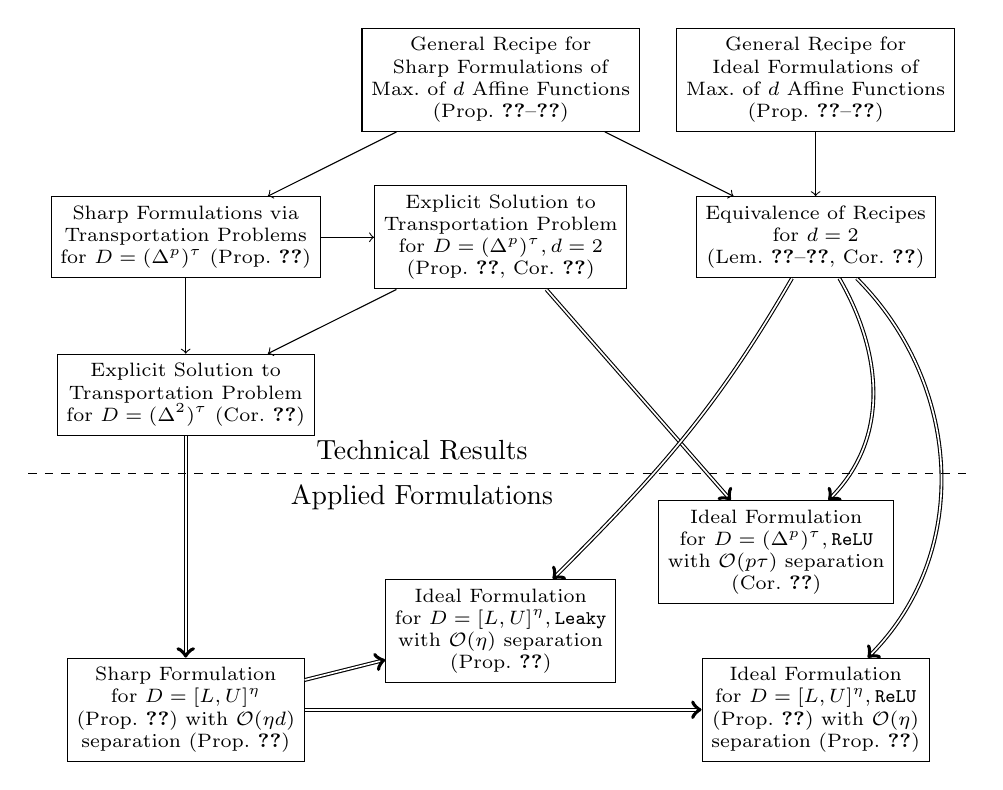
\begin{tikzpicture}[font=\scriptsize]
\node[draw, align=center] (A) at (8,2) {General Recipe for \\ Ideal Formulations of \\ Max.~of $d$ Affine Functions\\ (Prop.~\ref{prop:max_ideal_set_primal}--\ref{prop:max_ideal_set_dual})};
\node[draw, align=center] (B) at (4,2) {General Recipe for \\ Sharp Formulations of \\ Max.~of $d$ Affine Functions\\ (Prop.~\ref{prop:max_sharp_set_primal}--\ref{prop:max_sharp_set_dual})};
\node[draw, align=center] (C) at (8,0) {Equivalence of Recipes \\ for $d=2$ \\ (Lem.~\ref{lem:max_2_ideal_lb}--\ref{lem:max_2_ideal_ub}, Cor.~\ref{cor:max_2_ideal_general})};
\draw[->](A)--(C);
\draw[->](B)--(C);
\node[draw, align=center] (D) at (0,0) {Sharp Formulations via \\ Transportation Problems \\ for $D=(\Delta^p)^{\tau}$ (Prop.~\ref{prop:transportationDuality})};
\draw[->](B)--(D);
\node[draw, align=center] (E) at (4,0) {Explicit Solution to \\ Transportation Problem \\ for $D=(\Delta^p)^{\tau},d=2$ \\ (Prop.~\ref{prop:simplicesD2Explicit}, Cor.~\ref{cor:simplicesD2Result})};
\draw[->](D)--(E);
\node[draw, align=center] (H) at (0,-2) {Explicit Solution to \\ Transportation Problem \\ for $D=(\Delta^2)^{\tau}$ (Cor.~\ref{cor:simplicesP2})};
\draw[->](D)--(H);
\draw[->](E)--(H);
\node[draw, align=center] (F) at (7.5,-4) {Ideal Formulation \\ for $D=(\Delta^p)^{\tau},\ReLu$ \\ with $\mathcal{O}(p\tau)$ separation \\ (Cor.~\ref{cor:simplicesD2ReLU})};
\draw[->, double] (C) to [out=300,in=45] (F);
\draw[->, double](E)--(F);
\node[draw, align=center] (G) at (0,-6) {Sharp Formulation \\ for $D=[L,U]^{\eta}$ \\ (Prop.~\ref{prop:max_sharp}) with $\mathcal{O}(\eta d)$ \\ separation (Prop.~\ref{prop:max_sharp_sep})};
\draw[->, double](H)--(G);
\node[draw, align=center] (I) at (4,-5) {Ideal Formulation \\ for $D=[L,U]^{\eta},\Leaky$ \\ with $\mathcal{O}(\eta)$ separation \\ (Prop.~\ref{prop:ideal-leaky-relu})};
\draw[->, double](C) to [out=240,in=45] (I);
\node[draw, align=center] (J) at (8,-6) {Ideal Formulation \\ for $D=[L,U]^{\eta},\ReLu$ \\ (Prop.~\ref{prop:ideal-relu}) with $\mathcal{O}(\eta)$ \\ separation (Prop.~\ref{prop:relu-separation})};
\draw[->, double](C) to [out=315,in=45] (J);
\draw[->, double](G)--(I);
\draw[->, double](G)--(J);
\node at (3,-2.7) {\normalsize Technical Results};
\node at (3,-3.3) {\normalsize Applied Formulations};
\draw[dashed](-2,-3)--(10,-3);
\end{tikzpicture}
\caption{A roadmap of our results.  The single arrows depict dependencies between our technical results, while the double arrows depict the way in which we use these results to establish our applied formulations in the paper.
%(which are double-boxed).
Notationally, \blue{$d$ is the number of pieces of the piecewise linear function,} $[L,U]^\eta$ is an $\eta$-dimensional box, and $(\Delta^p)^\tau$ refers to a product of $\tau$ simplices, each with $p$ components.} %Additionally, we show that most of our formulations do not contain redundant constraints (Prop.~\ref{prop:simplicesD2FacetDefining}).}
\label{fig:results}
\end{figure}

% In Section~\ref{sec:relu}, we take an extended look at the ReLU, the simplest and most popular activation function in the deep learning community. In Section~\ref{sec:other-univariate}, we apply similar techniques to other univariate activation units: the leaky ReLU, the clipped ReLU, and the hard tanh unit. In Section~\ref{sec:max}, we turn our attention to the maximum of $d$ affine functions, a simple multivariate nonlinearity with widespread usage, especially in image classification networks where it manifests itself as the reduce max and max pooling nonlinearities.

% Our contributions in these three sections include a number of ideal MIP formulations for the ReLU, the leaky ReLU, and the maximum of two affine functions. We show that none of the constraints in these formulations are redundant (modulo variable bounds). We also provide strong MIP formulations for the clipped ReLU, the hard tanh unit, and the maximum of $d$ affine functions for general $d$. These formulations all have exponentially many constraints. However, we show that there are simple procedures to generate violated inequalities, as-needed, in time linear in the input dimension.

\subsection{Relevant prior work}\label{sec:lit-review}

In recent years a number of authors have used MIP formulations to model trained neural networks~\cite{Bunel:2017,Cheng:2017,Dutta:2017,Fischetti:2018,Huchette:2018,Kumar:2019,Lomuscio:2017,Say:2017,Serra:2018a,Serra:2018,Tjeng:2017,Wu:2017,Xiao:2018}, mostly applying big-$M$ formulation techniques to ReLU-based networks.
When applied to a single neuron of the form \eqref{eqn:single-neuron}, these big-$M$ formulations will not be ideal or offer an exact convex relaxation; see Example~\ref{ex:relu-big-M} for an illustration. Additionally, a stream of literature in the deep learning community has studied convex relaxations~\cite{Bastani:2016,Dvijotham:2018a,Ehlers:2017,Raghunathan:2018,Salman:2019}, primarily for verification tasks.
Moreover, some authors have investigated how to use convex relaxations within the training procedure in the hopes of producing neural networks with a priori robustness guarantees~\cite{Dvijotham:2018,Wong:2017,Wong:2018}.

\blue{The usage of mathematical programming in deep learning, specifically for training predictive models, has also been investigated in \cite{bienstock2018principled}.}
Beyond \blue{mathematical programming} and convex relaxations, a number of authors have investigated other algorithmic techniques for modeling trained neural networks in optimization problems, drawing primarily from the satisfiability, constraint programming, and global optimization communities~\cite{Bartolini:2011,Bartolini:2012,Katz:2017,Lombardi:2016,Schweidtmann:2018}.
\blue{Throughout this stream of the literature, there is discussion of the performance for specific subclasses of neural network models, including}
 binarized~\cite{Khalil:2018} or input convex~\cite{Amos:2017} neural networks.
\blue{Improving our formulations for specific subclasses of neural networks would constitute interesting future work.}
%Broadly, our work fits into a growing body of research in prescriptive analytics and specifically the ``predict, then optimize'' framework, which considers how to embed trained machine learning models into optimization problems~\cite{Bertsimas:2014k,Biggs:2017,Deng:2018,Donti:2017,Elmachtoub:2017,Hertog:2016,Misic:2017}.

\blue{Outside of applications in machine learning}, the formulations presented in this paper also have connections with existing structures studied in the MIP and constraint programming communities, like indicator variables, on/off constraints, and convex envelopes~\cite{Atamturk:2018,Belotti:2015,Bonami:2015,Hijazi:2011,Hijazi:2014,Tawarmalani:2002}.
\blue{Finally, this paper has connections with distributionally robust optimization, in that the primal-dual pair of sharp formulations presented can be viewed as equivalent to the discrete sup-sup duality result \cite{chen2018distributionally} for the marginal distribution model \cite{haneveld1986robustness,natarajan2009persistency,Weiss}.}

\subsection{Starting assumptions and notation} \label{sec:assumptions}
We use the following notational conventions throughout the paper.
\begin{itemize}
    \item The nonnegative orthant: $\bbR_{\geq 0} \defeq \Set{x \in \bbR | x \geq 0}$.
    \item The \blue{$n$}-dimensional simplex: $\Delta^{\blue{n}} \defeq \Set{ x \in \bbR^{\blue{n}}_{\geq 0} | \sum_{i=1}^{\blue{n}} x_i = 1}$.
    \item The set of integers from $1$ to $n$: $\llbracket n \rrbracket = \{1, \ldots, n\}$.
    \item ``Big-$M$'' coefficients: $M^+(f;D) \defeq \max_{x \in D} f(x)$ and $M^-(f;D) \defeq \min_{x \in D} f(x)$.
    % \item The support of a vector: $\supp(w) \defeq \Set{ i \in \llbracket \eta \rrbracket | w_i \neq 0}$.
    % \item For multi-dimensional (potentially ragged) arrays, we use colon syntax to denote a full slice along the given axis. For example, $x_{:,j,:} = ((x_{i,j,k})_{k=1}^{p_i})_{i=1}^{d}$ is the slice where $j$ is constant and the inner-most axis length, $p_i$, is dependent on the index $i$. \cnote{As far as I can tell, we only use this notation at three places: (15), (16), Prop.7. I think it might be better to just use the more bulky notation instead of defining this.}
    \item The dilation of a set: if $z \in \bbR_{\geq 0}$ and $D \subseteq \bbR^\eta$, then $z \cdot D \defeq \Set{ z x | x \in D}$.\footnote{Note that if $D = \Set{x \in \mathbb{R}^\eta | Ax \leq b}$ is polyhedral, then $z \cdot D = \Set{x \in \mathbb{R}^\eta | Ax \leq bz}$.}
\end{itemize}

Furthermore, we will make the following simplifying assumptions.

\begin{assumption}
    The input domain $D$ is a bounded polyhedron.
\end{assumption}

While a bounded input domain assumption will make the formulations and analysis considerably more difficult than the unbounded setting (see \cite{Atamturk:2018} for a similar phenomenon), it ensures that standard MIP representability conditions are satisfied (e.g. \cite[Section 11]{Vielma:2015}). Furthermore, variable bounds are natural for many applications (for example in verification problems), and are absolutely essential for ensuring reasonable dual bounds.

\begin{assumption} \label{ass:amphibious}
    Each neuron is \emph{irreducible}: for any $k \in \llbracket d \rrbracket$, there exists some $x \in D$ where $f^k(x) > f^\ell(x)$ for each $\ell \neq k$.
            % \item Each neuron is \emph{strictly active}: for any $i \in \llbracket d \rrbracket$, 
        %     \[
        %         \gr(\emph{\NL{}} \circ (f^1,\ldots,f^d); D) \neq \gr(\emph{\NL{}} \circ (f^1,\ldots,f^{i-1},f^{i+1},\ldots,f^d); D).
        %     \]
\end{assumption}

Observe that if a neuron is not irreducible, this means that it is unnecessarily complex, and one or more of the affine functions can be completely removed. Moreover, the assumption can be verified in polynomial time via $d$ LPs by checking if $\max_{x,\Delta} \Set{\Delta | x \in D,\ \Delta \leq f^k(x) - f^\ell(x)\ \forall \ell \neq k} > 0$ for each $k \in \llbracket d \rrbracket$. In the special case where $d = 2$ (e.g. ReLU) and $D$ is a box, this can be done in linear time.  Finally, if the assumption does not hold, it will not affect the validity of the formulations or cuts derived in this work, though certain results pertaining to non-redundancy or facet-defining properties may no longer hold.
% Observe that if a neuron is not irreducible, this means that it is unnecessarily complex, and one or more of the affine functions can be completely removed. Moreover, the assumption can be verified in polynomial time by solving $d$ LPs, since it is equivalent to the condition 
% \[
%     \max_{x,\Delta} \Set{\Delta | x \in D,\ \Delta \leq f^k(x) - f^\ell(x)\ \forall \ell \neq k} > 0
% \]
% for all $k \in \llbracket d \rrbracket$. In the special case where $d = 2$ (e.g. ReLU) and $D$ is a box, this can be checked in linear time.  Finally, if the assumption does not hold, it will not affect the validity of the formulations or cuts derived in this work, though certain results pertaining to non-redundancy or facet-defining properties may no longer hold.

% Define $\breve{L}, \breve{U} \in \bbR^\eta$ such that, for each $i \in \llbracket \eta \rrbracket$,
% \[
%     \breve{L}_i = \begin{cases} L_i & \text{ if } w_i \geq 0 \\ U_i & \text{ if } w_i < 0 \end{cases} \quad \text{ and } \quad \breve{U}_i = \begin{cases} U_i & \text{ if } w_i \geq 0 \\ L_i & \text{ if } w_i < 0 \end{cases}.
% \]
% This definition implies that $w_i \breve{L}_i \leq w_i \breve{U}_i$ for each $i$, which simplifies the handling of negative weights $w_i < 0$. Take the values $M^+(f) \defeq \max_{\tilde{x} \in [L,U]} f(\tilde{x}) \equiv w \cdot \breve{U} + b$ and $M^-(f) \defeq \min_{\tilde{x} \in [L,U]} f(\tilde{x}) \equiv w \cdot \breve{L} + b$. 

% \TODO{Define simplex $\Delta$, sync with Will's definition.}

% We say that \emph{strict activity} holds for a given (???) neuron $\gr(\ReLu{} \circ f; [L,U])$ if $M^-(f) < 0 < M^+(f)$, or in other words, if $\gr(\ReLu{} \circ f; [L,U])$ is not equal to either $\gr(0; [L,U])$ or $\gr(f; [L,U])$. We assume for the remainder that strict activity holds for each ReLU neuron. This assumption is not onerous, as otherwise, the nonlinearity can be replaced by an affine function (either $0$ or $w \cdot x + b$). Moreover, strict activity can be verified or disproven in time linear in $\eta$.
% --- end section-1.tex ---
% --- begin section-2.tex ---
\section{Motivating example: The ReLU nonlinearity over a box domain} \label{sec:relu}

\blue{
Since the work of Glorot et al.~\cite{glorot2011deep}, the ReLU neuron has become the workhorse of deep learning models. Despite the simplistic ReLU structure, neural networks formed by ReLU neurons are easy to train, reason about, and can model any continuous piecewise linear function \cite{arora2016understanding}.
Moreover, they can approximate any continuous, non-linear function to an arbitrary precision under a bounded width \cite{hanin2017universal}.

Accordingly, the general problem of maximizing (or minimizing) the output of a trained ReLU network is NP-hard \cite{Katz:2017}.
Nonetheless, in this section we present the strongest possible MIP formulations for a single ReLU neuron without continuous auxiliary variables. As discussed at the end of Section~\ref{sec:preliminaries} and corroborated in the computational study in Section~\ref{sec:computational}, this leads to faster solve times for the entire ReLU network in practice.
}

\subsection{A big-$M$ formulation} \label{ssec:relu-standard-formulations}

To start, we will consider the ReLU in the simplest possible setting: where the input is univariate. Take the two-dimensional set $\gr(\ReLu{}; [l,u])$, where $[l,u]$ is some interval in $\bbR$ containing zero. It is straightforward to construct an ideal formulation for this univariate ReLU.

\begin{proposition}
    An ideal formulation for $\gr(\emph{\ReLu{}}; [l,u])$ is:
\begin{subequations} \label{eqn:univariate-max-big-M}
\begin{align}
    y &\geq x \label{eqn:univariate-max-big-M-1} \\
    y &\leq x - l(1-z) \\
    y &\leq uz \\
    (x,y,z) &\in \bbR \times \bbR_{\geq 0} \times [0,1] \label{eqn:univariate-max-big-M-4} \\
    z &\in \{0,1\}.
\end{align}
\end{subequations}
\end{proposition}
\begin{proof}
    Follows from inspection, or as a special case of Proposition~\ref{prop:ideal-relu} to be presented in Section~\ref{ssec:relu-box}.
\qed \end{proof}

A more realistic setting would have an \blue{$\eta$-variate} ReLU nonlinearity whose input is some \blue{$\eta$-variate} affine function $f : [L,U] \to \bbR$ \blue{where $L,U\in \bbR^\eta$ and $[L,U]\defeq\Set{ x \in \bbR^\eta | L_i \leq  x_i \leq U_i\  \forall i\in \llbracket \eta \rrbracket} $} \blue{(i.e. the $\eta$-variate ReLU nonlinearity given by $\ReLu{} \circ f$)}. The \blue{ \emph{box-input}  $[L,U]$} corresponds to known (finite) bounds on each component, which can typically be efficiently computed via interval arithmetic or other standard methods.

Observe that we can model the \blue{graph} of the  \emph{\blue{$\eta$-variate} ReLU \blue{neuron}} as a simple composition of \blue{the graph of} a univariate ReLU \blue{activation function} and an \blue{$\eta$-variate} affine function:
\begin{equation}
  \blue{\gr\left(\ReLu{} \circ f;[L,U]\right)} =  \Set{ (x,y)\blue{\in\bbR^{\eta+1}} | \begin{array}{c}
        (f(x),y) \in \gr\left(\ReLu{}; [\blue{m^-,m^+}]\right) \\
        L \leq x \leq U
    \end{array}
    },
\end{equation}
\blue{where $m^-\defeq M^-(f; [L,U])$ and $m^+\defeq M^+(f; [L,U])$}.
Using formulation~\eqref{eqn:univariate-max-big-M} as a submodel, we can write a formulation for the ReLU over a box domain as:
\begin{subequations} \label{eqn:relu-big-M}
\begin{align}
    y &\geq f(x) \\
    y &\leq f(x) - M^-(f;[L,U]) \cdot (1-z) \label{eqn:relu-big-M-2} \\
    y &\leq M^+(f;[L,U]) \cdot z \label{eqn:relu-big-M-3} \\
    (x,y,z) &\in [L,U] \times \bbR_{\geq 0} \times [0,1] \\
    z &\in \{0,1\}.
\end{align}
\end{subequations}
This is the approach taken recently in the bevy of papers referenced in Section~\ref{sec:lit-review}. Unfortunately, after the composition with the affine function $f$ over a box input domain, this formulation is no longer sharp.

\begin{example} \label{ex:relu-big-M}
    If $f(x) = x_1 + x_2 - 1.5$, formulation \eqref{eqn:relu-big-M} for $\gr(\ReLu{} \circ f; [0,1]^2)$ is
    \begin{subequations}
    \begin{align}
        y &\geq x_1 + x_2 - 1.5 \label{eqn:relu-example-1} \\ 
        y &\leq x_1 + x_2 - 1.5 + 1.5(1-z) \\
        y &\leq 0.5z \\
        (x,y,z) &\in [0,1]^2\times \bbR_{\geq 0} \times [0,1] \label{eqn:relu-example-5} \\
        z &\in \{0,1\}.
    \end{align}
    \end{subequations}
    The point $(\hat{x},\hat{y},\hat{z}) = ((1,0),0.25,0.5)$ is feasible for the LP relaxation (\ref{eqn:relu-example-1}-\ref{eqn:relu-example-5}). However, observe that the inequality $y \leq 0.5x_2$ is valid for $\gr(\ReLu{} \circ f; [0,1]^2)$, but is violated by $(\hat{x},\hat{y})$. Therefore, the formulation does not offer an exact convex relaxation (and, hence, is not ideal). See Figure~\ref{fig:relu} for an illustration: on the left, of the big-$M$ formulation projected to $(x,y)$-space, and on the right, the tightest possible convex relaxation.
    % The point $(\hat{x},\hat{y},\hat{z}) = ((1,0),0.25,0.5)$ is feasible for the LP relaxation (\ref{eqn:relu-example-1}-\ref{eqn:relu-example-5}); however, $(\hat{x},\hat{y}) \equiv ((1,0),0.25)$ is not in $\Conv(\gr(\ReLu{} \circ f; [0,1]^2))$, and so the formulation does not offer an exact convex relaxation (and, hence, is not ideal). See Figure~\ref{fig:relu} for an illustration: on the left, of the big-$M$ formulation projected to $(x,y)$-space, and on the right, the tightest possible convex relaxation.
\end{example}

\tikzstyle{yzx} = [
  x={(1.2*.9625cm, 1.2*.9625cm)},
  y={(1.2*2.5cm, 0cm)},
  z={(0cm, 1.2*2.5cm)},
]

\begin{figure}
    \centering
    \begin{tikzpicture}[yzx]
        \draw [->, dashed, line width=1] (0,0,0) -- (1.2,0,0);
        \draw [->, dashed, line width=1] (0,0,0) -- (0,1.2,0);
        \draw [->, dashed, line width=1] (0,0,0) -- (0,0,0.7);
        \node[above right] at (1.2,-.075,0) {$x_2$};
        \node[right] at (0,1.2,0) {$x_1$};
        \node[above] at (0,0,.7) {$y$};
        \coordinate (LL) at (0,0,0);
        \coordinate (UL) at (1,0,0);
        \coordinate (LU) at (0,1,0);
        \coordinate (UU) at (1,1,0.5);
        \coordinate (UM) at (1,0.5,0);
        \coordinate (MU) at (0.5,1,0);
        \coordinate (E1) at (1,0,1/4);
        \coordinate (E2) at (0,1,1/4);

        \draw [fill=gray!80] (LL) -- (UL) -- (UM) -- (MU) -- (LU) -- cycle;
        \draw [fill=gray!80] (UU) -- (UM) -- (MU) -- cycle;
        \draw (LL) -- (E2) -- (UU) -- (E1) -- cycle;
        \draw (LL) -- (UL) -- (E1) -- cycle;
        \draw (LL) -- (LU) -- (E2) -- cycle;
        
        \begin{scope}[canvas is yz plane at x=0]
            \draw [fill] (1,1/4) circle [radius=.025];
        \end{scope}
    \end{tikzpicture} \hspace{2em}
    \begin{tikzpicture}[yzx]
        \draw [->, dashed, line width=1] (0,0,0) -- (1.2,0,0);
        \draw [->, dashed, line width=1] (0,0,0) -- (0,1.2,0);
        \draw [->, dashed, line width=1] (0,0,0) -- (0,0,0.7);
        \node[above right] at (1.2,-0.075,0) {$x_2$};
        \node[right] at (0,1.2,0) {$x_1$};
        \node[above] at (0,0,.7) {$y$};
        \coordinate (LL) at (0,0,0);
        \coordinate (UL) at (1,0,0);
        \coordinate (LU) at (0,1,0);
        \coordinate (UU) at (1,1,0.5);
        \coordinate (UM) at (1,0.5,0);
        \coordinate (MU) at (0.5,1,0);
        
        \draw [fill=gray!80] (LL) -- (UL) -- (UM) -- (MU) -- (LU) -- cycle;
        \draw [fill=gray!80] (UU) -- (UM) -- (MU) -- cycle;
        \draw (LL) -- (UL) -- (UU) -- cycle;
        \draw (LL) -- (LU) -- (UU) -- cycle;
        
        \begin{scope}[canvas is yz plane at x=0]
            \draw [fill] (1,1/4) circle [radius=.025];
        \end{scope}
    \end{tikzpicture}
    \caption{For $f(x) = x_1 + x_2 - 1.5$: \textbf{(Left)} $\Conv(\gr(\ReLu{} \circ f; [0,1]^2))$, and \textbf{(Right)} the projection of the big-$M$ formulation \eqref{eqn:relu-big-M} to $(x,y)$-space, where we mark the point $(x,y) = ((1,0),0.25)$ that is not in the convex hull, but is valid for the projection of the big-$M$ LP relaxation (\ref{eqn:relu-example-1}-\ref{eqn:relu-example-5}).}
    \label{fig:relu}
\end{figure}

Moreover, the integrality gap of \eqref{eqn:relu-big-M} can be arbitrarily bad, even in fixed dimension $\eta$.

\begin{example}
Fix $\gamma \in \bbR_{\geq 0}$ and even $\eta \in \bbN$.
Take the affine function $f(x) = \sum_{i=1}^\eta x_i$, the input domain $[L,U] = [-\gamma,\gamma]^\eta$, and $\hat{x} = \gamma \cdot (1,-1,\cdots,1,-1)$ as a scaled vector of alternating positive and negative ones. We can check that $(\hat{x},\hat{y},\hat{z}) = (\hat{x},\frac{1}{2}\gamma\eta,\frac{1}{2})$ is feasible for the LP relaxation of the big-$M$ formulation \eqref{eqn:relu-big-M}. Additionally, $f(\hat{x}) = 0$, and for any $\tilde{y}$ such that $(\hat{x},\tilde{y}) \in \Conv(\gr(\ReLu{} \circ f; [L,U]))$, then $\tilde{y} = 0$ necessarily. Therefore, there exists a fixed point $\hat{x}$ in the input domain where the tightest possible convex relaxation (for example, from a sharp formulation) is exact, but the big-$M$ formulation deviates from this value by at least $\frac{1}{2}\gamma\eta$.
\end{example}

Intuitively, this example suggests that the big-$M$ formulation can be particularly weak around the boundary of the input domain, as it cares only about the value $f(x)$ of the affine function, and not the particular input value $x$.

\subsection{An ideal extended formulation} \label{ssec:ideal-extended}

It is possible to produce an ideal \emph{extended} formulation for the ReLU neuron by introducing a modest number of auxiliary continuous variables:
\begin{subequations} \label{eqn:relu-ideal-extended}
\begin{align}
    (x,y) &= (x^0,y^0) + (x^1,y^1) \label{eqn:relu-ideal-extended-1} \\
    y^0 &= 0 \geq w \cdot x^0 + b(1-z) \label{eqn:relu-ideal-extended-2} \\
    y^1 &= w \cdot x^1 + bz \geq 0 \label{eqn:relu-ideal-extended-3} \\
    L(1-z) &\leq x^0 \leq U(1-z)\label{eqn:relu-ideal-extended-4} \\
    Lz &\leq x^1 \leq Uz \label{eqn:relu-ideal-extended-5} \\
    z &\in \{0,1\},
\end{align}
\end{subequations}
This is the standard ``multiple choice'' formulation for piecewise linear functions~\cite{Vielma:2009a}, which can also be derived from techniques due to Balas~\cite{Balas:1985,Balas:1998}.% We can interpret the LP relaxation of~\eqref{eqn:relu-ideal-extended} as expressing $(x,y)$ as a convex combination of points $\frac{1}{1-z}(x^0, y^0)$ and $\frac{1}{z}(x^1,y^1)$, one in each piece of the ReLU.

Although the multiple choice formulation offers the tightest possible convex relaxation for a single neuron, it requires a copy $x^0$ of the input variables (the copy $x^1$ can be eliminated using the equations \eqref{eqn:relu-ideal-extended-1}). This means that when this formulation is applied to every neuron in the network to formulate $\NN{}$, the total number of continuous variables required is $m_0 + \sum_{i=1}^{r} (m_{i-1}+1)m_{i}$, where $m_i$ is the number of neurons in layer $i$. In contrast, the big-$M$ formulation requires only $m_0 + \sum_{i=1}^r m_i$ continuous variables to formulate the entire network. As we will see in Section~\ref{sec:computational}, the quadratic growth in size of the extended formulation can quickly become burdensome. Additionally, a folklore observation in the MIP community is that multiple choice formulations tend to not perform as well as expected in simplex-based branch-and-bound algorithms, likely due to degeneracy introduced by the block structure of the formulation~\cite{Vielma:2018}.

\subsection{An ideal MIP formulation without auxiliary continuous variables} \label{ssec:ideal-relu}

In this work, our most broadly useful contribution is the derivation of an ideal MIP formulation for the ReLU nonlinearity over a box domain that is non-extended; that is, it does not require additional auxiliary variables as in formulation \eqref{eqn:relu-ideal-extended}. We informally summarize this main result as follows.

% \begin{quote}
%     \emph{\textbf{Informal statement of main results for ReLU networks:} There exists an explicit ideal nonextended formulation for the ReLU nonlinearity over a box domain, i.e. it requires only a single auxiliary binary variable. It has an exponential (in $\eta$) number of inequality constraints, each of which are facet-defining. However, it is possible to separate over this family of inequalities in time scaling linearly in $\eta$.}
% \end{quote}

\medskip
\begin{theo*} \label{thm:informal}
    There exists an explicit ideal nonextended formulation for the  \blue{$\eta$-variate} ReLU nonlinearity over a box domain, i.e. it requires only a single auxiliary binary variable. It has an exponential (in $\eta$) number of inequality constraints, each of which are facet-defining. However, it is possible to separate over this family of inequalities in time scaling linearly in $\eta$.
\end{theo*}
\medskip

We defer the formal statement and proof to Section~\ref{ssec:relu-box}, for after we have derived the requisite machinery. This is also the main result for the extended abstract version of this work~\cite{Anderson:2019}, where it is derived through alternative means.

% We defer the formal statement and proof to Section~\ref{ssec:relu-box}, for after we have derived the requisite machinery, for this and a number of related results. However, we do note this serves as the main result for the extended abstract version of this work~\cite{Anderson:2019}, where it is derived through alternative means.
% --- end section-2.tex ---
% --- begin section-3.tex ---
\section{Our general machinery: Formulations for the maximum of $d$ affine functions} \label{sec:max}

We will state our main structural results in the following generic setting. Take the maximum operator $\Max{}(v_1,\ldots,v_d) = \max_{i=1}^d v_i$ over $d$ scalar inputs. We study the composition of this nonlinearity with $d$ affine functions $f^i : D \to \bbR$ with $f^i(x) = w^i \cdot x + b^i$, all sharing some bounded polyhedral domain $D$:
\[
    \Smax \defeq \gr(\Max{} \circ (f^1,\ldots,f^d); D) \equiv \Set{ (x,y) \in D \times \bbR | y = \max_{i=1}^d f^i(x) },
\]
This setting subsumes the ReLU over box input domain presented in Section~\ref{sec:relu} as a special case with $d=2$, $f^2(x) = 0$, and $D = [L,U]$. It also covers a number of other settings arising in modern deep learning, either by making $D$ more complex (e.g. one-hot encodings for categorical features), or by increasing $d$ (e.g. max pooling neurons often used in convolutional networks for image classification tasks~\cite{Boureau:2010}, or in maxout networks~\cite{Goodfellow:2013}).

In this section, we present structural results that characterize the \emph{Cayley embedding}~\cite{Huber:2000,Vielma:2016,Vielma:2018,Weibel:2007} of $\Smax$. Take the set
\[
    \Scayley \defeq \bigcup_{k=1}^d \Set{ (x,f^k(x),{\bf e}^k) | x \in D_{|k}},
\]
where ${\bf e}^k$ is the unit vector where the $k$-th element is 1, and for each $k \in \llbracket d \rrbracket$,
\begin{align*}
D_{|k} &\defeq \Set{ x \in D | k \in \arg\max_{\ell=1}^d f^\ell(x)} \equiv \Set{x \in D | w^k \cdot x + b^k \geq w^\ell \cdot x + b^\ell \ \forall \ell \neq k }
\end{align*}
is the portion of the input domain $D$ where $f^k$ attains the maximum. The \emph{Cayley embedding} of $\Smax$ is the convex hull of this set: $\Rcayley \defeq \Conv(\Scayley)$.
% We assume throughout this section that $D_{|k}$ is nonempty for all $k \in \llbracket d \rrbracket$. If it is empty, then the function $f^k(x)$ has no impact on the \Max{} unit and we may remove it. We also implicitly assume that the domain polytope $D$ considered in this section are nonempty.

The following straightforward observation holds directly from definition.

\begin{observation}
The set $\Rcayley$ is a bounded polyhedron, and an ideal formulation for $\Smax$ is given by the system $\Set{(x,y,z) \in \Rcayley | z \in \{0,1\}^d}$.
\end{observation}

Therefore, if we can produce an explicit inequality description for $\Rcayley$, we immediately have an ideal MIP formulation for $\Smax$. Indeed, we have already seen an extended representation in \eqref{eqn:relu-ideal-extended} when $d=2$, which we now state in the more general setting (projecting out the superfluous copies of $y$).

\begin{proposition}\label{prop:extended-formulation-cayley}
An ideal MIP formulation for $\Smax$ is:
    \begin{subequations}\label{eqn:extended-formulation}
    \begin{alignat}{2}
    (x,y) &= \sum_{k=1}^d (\tx^k, w^k \cdot \tx^k + b^kz_k) \label{eqn:extended-formulation-1} \\
    % x &= \sum_{k=1}^d \tx^k \label{eqn:extended-formulation-1} \\
    % y &= \sum_{k=1}^d (w^k \cdot \tx^k + b^kz_k)\\
    % w^k \cdot \tx^k + b^kz_k &\geq w^\ell \cdot \tx^k + b^\ell z_k &\quad &\forall k,\ell \in \llbracket d \rrbracket:\: k \neq \ell \label{eqn:ideal-max-piece}\\
    % \tx^k &\in z_k \cdot D &\quad &\forall k \in \llbracket d \rrbracket \label{eqn:extended-formulation-4} \\
    \tx^k &\in z_k \cdot D_{|k} &\quad &\forall k \in \llbracket d \rrbracket \label{eqn:extended-formulation-4} \\
    z &\in \Delta^d \label{eqn:extended-formulation-5} \\
    z &\in \{0,1\}^d.
    \end{alignat}
    \end{subequations}
    Denote its LP relaxation by $\Rextended = \Set{(x,y,z,\tx^1,\ldots,\tx^k) | (\ref{eqn:extended-formulation-1}-\ref{eqn:extended-formulation-5})}$. Then $\Proj_{x,y,z}(\Rextended) = \Rcayley$.
\end{proposition}
\blue{
\begin{proof}
Follows directly from results in \cite{Balas:1985,Balas:1998}.
\qed\end{proof}}
Although this formulation is ideal and polynomially-sized, this extended formulation can exhibit poor practical performance, as noted in Section~\ref{ssec:ideal-extended} and corroborated in the computational experiments in Section~\ref{sec:computational}. Observe that, from definition, constraint \eqref{eqn:extended-formulation-4} for a given $k \in \llbracket d \rrbracket$ is equivalent to the set of constraints $\tx^k \in z_k \cdot D$ and $w^k \cdot \tx^k + b^kz_k \geq w^\ell \cdot \tx^k + b^\ell z_k$ for each $\ell \neq k$.
%Note that taken together, (\ref{eqn:ideal-max-piece}-\ref{eqn:extended-formulation-4}) are equivalent to the constraints $\tx^k \in z_k \cdot D_{|k}$ for each $k \in \llbracket d \rrbracket$.

\subsection{A recipe for constructing ideal formulations} \label{ssec:ideal-recipe}
Our goal in this section is to derive generic tools that allow us to build ideal formulations for $\Smax$ via the Cayley embedding.

\subsubsection{A primal characterization}

Our first structural result provides a characterization for the Cayley embedding. Although it is not an explicit polyhedral characterization, we will subsequently see how it can be massaged into a more practically amenable form.

Take the system
\begin{subequations}\label{eqn:max_ideal_set_primal}
\begin{align}
    y &\leq \bar{g}(x,z)\label{eqn:max_ideal_set_primal-1}\\
    y &\geq \ubar{g}(x,z)\label{eqn:max_ideal_set_primal-2}\\
    (x,y,z) &\in D \times \mathbb{R} \times \Delta^d,\label{eqn:max_ideal_set_primal-3}
\end{align}
\end{subequations}
where
\begin{align*}
    \bar{g}(x,z) \defeq \max_{\tx^1, \ldots, \tx^d}\Set{\sum_{k=1}^d w^k \cdot \tx^k + b^k z_k | \begin{array}{cc} x = \sum_k \tx^k & \\ \tx^k \in z_k \cdot D_{|k} &\ \forall k \in \llbracket d \rrbracket \end{array}}\hspace{0.45em}  \\
    \ubar{g}(x,z) \defeq \min_{\tx^1, \ldots, \tx^d}\Set{\sum_{k=1}^d w^k \cdot \tx^k + b^k z_k | \begin{array}{cc} x = \sum_k \tx^k & \\ \tx^k \in z_k \cdot D_{|k} &\ \forall k \in \llbracket d \rrbracket \end{array}},
\end{align*}
and define the set $\Rideal \defeq \Set{ (x,y,z) | \eqref{eqn:max_ideal_set_primal}}$. \blue{Note that $\Rideal$ can be thought of as \eqref{eqn:extended-formulation} with the $\tx^k$ variables implicitly projected out.}

\begin{proposition}\label{prop:max_ideal_set_primal}
    The set $\Rideal$ is polyhedral, and $\Rideal = \Rcayley$.
\end{proposition}
% \begin{proof}
% See Appendix~\ref{app:max_ideal_set_primal}.
% \qed\end{proof}
\begin{proof}
By Proposition~\ref{prop:extended-formulation-cayley}, it suffices to show that $\Rideal = \Proj_{x,y,z}(\Rextended)$. We start by observing that, as $\bar{g}$ (respectively $\ubar{g})$ is concave (resp. convex) in its imputs as it is the value function of a linear program (cf. \cite[Theorem 5.1]{Bertsimas:1997}). Therefore, the set of points satisfying \eqref{eqn:max_ideal_set_primal} is convex.

Let $(\hat{x}, \hat{y}, \hat{z})$ be an extreme point of $\Rideal$, which exists as $\Rideal$ is convex. Then it must satisfy either \eqref{eqn:max_ideal_set_primal-1} or \eqref{eqn:max_ideal_set_primal-2} at equality, as otherwise it is a convex combination of $(\hat{x}, \hat{y} - \epsilon, \hat{z})$ and $(\hat{x}, \hat{y} + \epsilon, \hat{z})$ for some $\epsilon > 0$. Take $\tx^1, \ldots, \tx^d$ that optimizes $\bar{g}(x,z)$ or $\ubar{g}(x,z)$, depending on which constraint is satisfied at equality. Then $(\hat{x}, \hat{y}, \hat{z}, \tx^1, \ldots, \tx^d) \in \Rextended$. In other words, $\text{ext}(\Rideal) \subseteq \Proj_{x,y,z}(\Rextended)$, and thus $\Rideal \subseteq \Proj_{x,y,z}(\Rextended)$ by convexity.

Conversely, let $(\hat{x},\hat{y},\hat{z},\tx^1,\ldots,\tx^d) \in \Rextended$. Then $\hat{y} = \sum_{k=1}^d (w^k \cdot \tx^k + b^k\hat{z}_k) \leq \bar{g}(\hat{x}, \hat{z})$, as $(\{\tx^k\}_{k=1}^d)$ is feasible for the optimization problem in $\bar{g}(x, z)$. %Likewise, $\hat{y} \geq \ubar{g}(\hat{x}, \hat{z})$, and the remaining constraints are also satisfied. Therefore, $(\hat{x}, \hat{y}, \hat{z}) \in \Rideal$.
Likewise, $\hat{y} \geq \ubar{g}(\hat{x}, \hat{z})$, and \eqref{eqn:max_ideal_set_primal-3} is trivially satisfied. Therefore, $(\hat{x}, \hat{y}, \hat{z}) \in \Rideal$.

Polyhedrality of $\Rideal$ then follows as $\Rcayley$ is itself a polyhedron.
\qed\end{proof}

Note that the input domain constraint $x \in D$ is implied by the constraints (\ref{eqn:max_ideal_set_primal-1})--(\ref{eqn:max_ideal_set_primal-2}), and therefore do not need to be explicitly included in this description. However, we include it here in our description for clarity. Moreover, observe that $\bar{g}$ is a function from $D \times \Delta^d$ to $\mathbb{R} \cup \{-\infty\}$, since the optimization problem may be infeasible, but is always bounded from above since $D$ is bounded. Likewise, $\ubar{g}$ is a function from $D \times \Delta^d$ to $\mathbb{R} \cup \{+\infty\}$.

% Note that the constraint $x\in D$ is implied by constraints (\ref{eqn:max_ideal_set_primal-1})--(\ref{eqn:max_ideal_set_primal-2}).
% This is because if $x\notin D$, then there cannot exist values of $\tx^k\in X^k_D$ such that $\sum_k\tx^kz_k=x$, in which case
% $\bar{g}(x,z)$ and $\ubar{g}(x,z)$ are understood to be $-\infty$ and $\infty$, respectively.
% In this case, no value of $y$ is feasible.

\subsubsection{A dual characterization}\label{sec:ideal_dual}

From Proposition~\ref{prop:max_ideal_set_primal}, we can derive a more useful characterization by applying Lagrangian duality to the LPs describing the envelopes $\bar{g}(x,z)$ and $\ubar{g}(x,z)$.

% \begin{lemma}\label{lem:max_ideal_set_dual}
% Define the following set:
% \begin{subequations}\label{eqn:max_ideal_set_dual}
% \begin{align}
%     \Sideal' := \{(x, y, z) :\ &y \leq \bar{\alpha} \cdot x + \sum_{k=1}^d \left(\max_{\tx^k \in X_D^k}\{(w^k - \bar{\alpha}) \cdot \tx^k\} + b^k\right)z_k\quad\forall \bar{\alpha} \in \mathbb{R}^n\label{eqn:max_ideal_set_dual-1}\\
%     &y \geq \ubar{\alpha} \cdot x + \sum_{k=1}^d \left(\min_{\tx^k \in X_D^k}\{(w^k - \ubar{\alpha}) \cdot \tx^k\} + b^k\right)z_k\quad\forall \ubar{\alpha} \in \mathbb{R}^n\label{eqn:max_ideal_set_dual-2}\\
%     &\sum_{k=1}^d z_k = 1 \\
%     &z \in [0,1]^d\}.
% \end{align}
% \end{subequations}

% Then $\Sideal' = \text{proj}_{x,y,z}(\Sdisj)$.

% \end{lemma}
\begin{proposition} \label{prop:max_ideal_set_dual}
The Cayley embedding $\Rcayley$ is equal to all $(x,y,z)$ satisfying
\begin{subequations}\label{eqn:max_ideal_set_dual}
\begin{align}
    y \leq \bar{\alpha} \cdot x + \sum_{k=1}^d \left(\max_{x^k \in D_{|k}}\{(w^k - \bar{\alpha}) \cdot x^k\} + b^k\right)z_k&\quad\forall \bar{\alpha} \in \mathbb{R}^\eta\label{eqn:max_ideal_set_dual-1}\\
    y \geq \ubar{\alpha} \cdot x + \sum_{k=1}^d \left(\min_{x^k \in D_{|k}}\{(w^k - \ubar{\alpha}) \cdot x^k\} + b^k\right)z_k&\quad\forall \ubar{\alpha} \in \mathbb{R}^\eta\label{eqn:max_ideal_set_dual-2}\\
    (x,y,z) \in D \times \mathbb{R} \times \Delta^d.
\end{align}
\end{subequations}
\end{proposition}
% \begin{proof}
% See Appendix~\ref{app:max_ideal_set_dual}.
% \qed\end{proof}
\begin{proof}
Consider the upper bound inequalities for $y$ in Proposition~\ref{prop:max_ideal_set_primal}, that is, \eqref{eqn:max_ideal_set_primal-1}. Now apply the change of variables $x^k \leftarrow \frac{\tx^k}{z_k}$ for each $k \in \llbracket d \rrbracket$ and, for all $(x,z)$, take the Lagrangian dual of the optimization problem in $\bar{g}(x,z)$ with respect to the constraint $x = \sum_k x^k z_k$. Note that the duality gap is zero since the problem is an LP. We then obtain that
\begin{align*}
    \bar{g}(x,z) &= \min_{\bar{\alpha}} \max_{x^k \in D_{|k}} \sum_{k=1}^d \left(w^k \cdot x^k + b^k\right) z_k + \bar{\alpha} \cdot \left(x - \sum_{k=1}^d x^k z_k\right) \notag\\
    &= \min_{\bar{\alpha}}\ \bar{\alpha} \cdot x + \sum_{k=1}^d \left(\max_{x^k \in D_{|k}}\{(w^k - \bar{\alpha}) \cdot x^k\} + b^k\right)z_k.
\end{align*}

In other words, we can equivalently express~\eqref{eqn:max_ideal_set_primal-1} via the family of inequalities~\eqref{eqn:max_ideal_set_dual-1}. The same can be done with~\eqref{eqn:max_ideal_set_primal-2}, yielding the set of inequalities~\eqref{eqn:max_ideal_set_dual-2}. Therefore, $\Set{(x,y,z) | \eqref{eqn:max_ideal_set_dual}} = \Proj_{x,y,z}(\Rextended) = \Rcayley$.
\qed\end{proof}

This gives an exact outer description for the Cayley embedding in terms of an infinite number of linear inequalities. Despite this, the formulation enjoys a simple, interpretable form: we can view the inequalities as choosing coefficients on $x$ and individually tightening the coefficients on $z$ according to explicitly described LPs. \blue{Similar to the relationship between \eqref{eqn:extended-formulation} and \eqref{eqn:max_ideal_set_primal}, \eqref{eqn:max_ideal_set_dual} can be seen as a simplification of the standard cut generation LP for unions of polyhedra \cite{Balas:1985,Balas:1998}.} In later sections, we will see that this decoupling is helpful to simplify (a variant of) this formulation for special cases.

Separating a point $(\hat{x}, \hat{y}, \hat{z})$ over~\eqref{eqn:max_ideal_set_dual-1} can be done by evaluating $\bar{g}(\hat{x},\hat{z})$ in the form~\eqref{eqn:max_ideal_set_dual-1} (and in the analogous form of $\ubar{g}(\hat{x},\hat{z})$ for~\eqref{eqn:max_ideal_set_dual-2}). As typically done when using Lagrangian relaxation, this optimization problem can be solved via a subgradient or bundle method, where each subgradient can be computed by solving the inner LP in~\eqref{eqn:max_ideal_set_dual-1} for all $x^k \in D_{|k}$. Observe that any feasible solution $\bar{\alpha}$ for the optimization problem in~\eqref{eqn:max_ideal_set_dual-1} yields a valid inequality. However, this optimization problem is unbounded when $(\hat{x}, \hat{z}) \notin \Proj_{x,z}(\Rcayley)$ (i.e. when the primal form of $\bar{g}(\hat{x}, \hat{z})$ is infeasible). In other words, as illustrated in Figure~\ref{fig:upper_bound_functions}, $\bar{g}$ is an \emph{extended} real valued function such that $\bar{g}({x}, {z})\in \mathbb{R}\cup \{-\infty\}$, so care must be taken to avoid numerical instabilities when separating a point $(\hat{x}, \hat{z})$ where $\bar{g}(\hat{x}, \hat{z})=-\infty$.\footnote{As is standard in a Benders' decomposition approach, we can address this by adding a \emph{feasibility cut} describing the domain of $\bar{g}$ (the region where it is finite valued) instead of an \emph{optimality cut} of the form \eqref{eqn:max_ideal_set_dual-1}.}

% evaluating it throgh unstable inequalities due to large coefficients in magnitude. A simple way to mitigate this in practice is to limit the number of iterations of the algorithm after violation is detected. \jpnote{I think this needs the details in the TODO below. However, given that we are not actually solving the lagrangian  problem maybe it's better to switch the focus of this discussion to the domain of $\bar{g}$ being smaller than $D$ (this domain is described by all feasibility cuts) and point to Figure 3. }

% \TODO{Continue this. Options: 1) Include coefficient for $y$ and normalize with unit ball (maybe a bit more convoluted than we want); 2) Say that we can take any inequality and do not worry about numerical issues; 3) Identify unbounded ray to generate feasibility cut (is this possible with subgradient descent)?}

\subsection{A recipe for constructing hereditarily sharp formulations}

Although Proposition~\ref{prop:max_ideal_set_dual} gives a separation-based way to optimize over $\Smax$, there are two potential downsides to this approach. First, it does not give us a explicit, finite description for a MIP formulation that we can directly pass to a MIP solver. Second, the separation problem requires optimizing over $D_{|k}$, which may be substantially more complicated than optimizing over $D$ (for example, if $D$ is a box).

Therefore, in this section we set our sights slightly lower and present a similar technique to derive \emph{sharp} MIP formulations for $\Smax$. Furthermore, we will see that our formulations trivially satisfy the hereditary sharpness property. In the coming sections, we will see how we can deploy these results in a practical manner, and study settings in which the simpler sharp formulation will also, in fact, be ideal.

\subsubsection{A primal characterization}

Consider the system
\begin{subequations}\label{eqn:max_sharp_set_primal}
\begin{align}
    y &\leq \bar{h}(x, z)\label{eqn:max_sharp_set_primal-1}\\
    y &\geq w^k \cdot x + b^k\quad\forall k \in \llbracket d \rrbracket \label{eqn:max_sharp_set_primal-2}\\
    (x,y,z) &\in D \times \mathbb{R} \times \Delta^d,
\end{align}
\end{subequations}
where
\begin{align*}
    \bar{h}(x, z) \defeq \max_{\tx^1, \ldots, \tx^d}\Set{\sum_{k=1}^d (w^k \cdot \tx^k + b^k z_k) | \begin{array}{cc} x = \sum_k \tx^k & \\ \tx^k \in z_k \cdot D &\ \forall k \in \llbracket d \rrbracket \end{array}}.
\end{align*}
Take the set $\Rsharp \defeq \Set{ (x,y,z) | \eqref{eqn:max_sharp_set_primal} }$.

It is worth dwelling on the differences between the systems~\eqref{eqn:max_ideal_set_primal} and \eqref{eqn:max_sharp_set_primal}. First, we have completely replaced the constraint \eqref{eqn:max_ideal_set_primal-2} with $d$ explicit linear inequalities \eqref{eqn:max_sharp_set_primal-2}. Second, when replacing $\bar{g}$ with $\bar{h}$ we have replaced the inner maximization over $D_{|k}$ with an inner maximization over $D$ (modulo constant scaling factors). As we will see in Section~\ref{ssec:max-cuts}, this is particularly advantageous when $D$ is trivial to optimize over (for example, a simplex or a box), allowing us to write these constraints in closed form, whereas optimizing over $D_{|k}$ may be substantially more difficult (i.e. requiring an LP solve).

Furthermore, we will show that while \eqref{eqn:max_sharp_set_primal} is not ideal, it is hereditarily sharp, and so in general may offer a strictly stronger relaxation than a standard sharp formulation. In particular, the formulation may be stronger than a sharp formulation constructed by composing a big-$M$ formulation, along with an exact convex relaxation in the $(x,y)$-space produced, for example, by studying the upper concave envelope of the function $\Max \circ (f^1,\ldots,f^d)$.

\begin{proposition} \label{prop:max_sharp_set_primal}
    The system describing $\Set{(x,y,z) \in \Rsharp | z \in \{0,1\}^d}$ is a hereditarily sharp MIP formulation of $\Smax$.
    % The set $\Rsharp$ is both valid and sharp for $\Smax$, in the sense that:
    % \begin{enumerate}
    %     \item $\Proj_{x,y}\left(\Rsharp \cap (\bbR^{\eta} \times \bbR \times \{0,1\}^d)\right) = \Smax$, and
    %     \item $\Proj_{x,y}(\Rsharp) = \Conv(\Smax)$.
    % \end{enumerate}
\end{proposition}

% \begin{proof}
% See Appendix~\ref{app:max_sharp_set_primal}.
% \qed\end{proof}

\begin{proof}
% For the result, we must show four properties: polyhedrality of $\Rsharp$, validity of the formulation whose LP relaxation is $\Rsharp$, sharpness, and then hereditary sharpness. We leave the proof of polyhedrality and validity to Appendix~\ref{app:max_sharp_set_primal} and prove sharpness and hereditary sharpness here.
For the result, we must show four properties: polyhedrality of $\Rsharp$, validity of the formulation whose LP relaxation is $\Rsharp$, sharpness, and then hereditary sharpness. We proceed in that order.

To show polyhedrality, consider a fixed value $(\hat{x},\hat{y},\hat{z})$ feasible for \eqref{eqn:max_sharp_set_primal}, and presume that we express the domain via the linear inequality constraints $D = \Set{x | Ax \leq c}$. First, observe that due to \eqref{eqn:max_sharp_set_primal-1} and \eqref{eqn:max_sharp_set_primal-2}, $\bar{h}(\hat{x},\hat{z})$ is bounded from below. Now, using LP duality, we may rewrite
\begin{align*}
    \bar{h}(\hat{x},\hat{z}) &= \max_{\tx^1, \ldots, \tx^d}\Set{\sum_{k=1}^d w^k \cdot \tx^k | \begin{array}{cc} \hat{x} = \sum_k \tx^k & \\ A \tx^k \leq \hat{z}_k c &\ \forall k \in \llbracket d \rrbracket \end{array}} + \sum_{k=1}^d b^k \hat{z}_k \\
    &= \min_{(\alpha, \beta^1, \ldots, \beta^k) \in R} \Set{ \alpha \cdot \hat{x} + \sum_{k=1}^d c \cdot \beta^k \hat{z}_k} + \sum_{k=1}^d b^k\hat{z}_k,
\end{align*}
where $R$ is a polyhedron that is \emph{independent of $\hat{x}$ and $\hat{z}$}. 
Therefore, as (a) the above optimization problem is linear with $\hat{x}$ and $\hat{z}$ fixed, and (b) $\bar{h}(\hat{x},\hat{z})$ is bounded from below, we may replace $R$ with $\ext(R)$ in the above optimization problem.
In other words, $\bar{h}(\hat{x},\hat{z})$ is equal to the minimum of a finite number of alternatives which are affine in $\hat{x}$ and $\hat{z}$. Therefore, $\bar{h}$ is a concave continuous piecewise linear function, and so $\Rsharp$ is polyhedral.

To show validity, we must have that $\Proj_{x,y}\left(\Rsharp \cap (\bbR^{\eta} \times \bbR \times \{0,1\}^d)\right) = \Smax$.
Observe that if $(\hat{x},\hat{y},\hat{z}) \in \Rsharp \cap (\bbR^{\eta} \times \bbR \times \{0,1\}^d)$, then $\hat{z} = {\bf e}^\ell$ for some $\ell \in \llbracket d \rrbracket$, and
\begin{align*}
    \bar{h}(\hat{x},\hat{z}) &= \max_{\tx^1, \ldots, \tx^d}\Set{\sum_{k=1}^d w^k \cdot \tx^k + b^\ell | \begin{array}{cc} \hat{x} = \sum_k \tx^k & \\ \tx^\ell \in D & \\ \tx^k = {\bf 0}^\eta &\forall k \neq \ell \end{array}} = w^\ell \hat{x} + b^\ell,
\end{align*}
where the first equality follows as $\tx^k = {\bf 0}^\eta$ for each $k \neq \ell$ (recall that if $D$ is bounded, then $0 \cdot D = \Set{x \in \bbR^\eta | Ax \leq 0} = \{{\bf 0}^\eta\}$).
Along with \eqref{eqn:max_sharp_set_primal-2}, this implies that $\hat{y} = w^\ell \cdot \hat{x} + b^\ell$, and that $\hat{y} \geq w^k \cdot \hat{x} + b^k$ for each $k \neq \ell$, giving the result.

To show sharpness, we must prove that $\Proj_{x,y}(\Rsharp) = \Conv(\Smax)$. First, recall from Proposition~\ref{prop:extended-formulation-cayley} that $\Conv(\Smax) = \Proj_{x,y}(\Rextended)$; thus, we state our proof in terms of $\Rextended$.
We first show that $\Proj_{x,y}(\Rextended) \subseteq \Proj_{x,y}(\Rsharp)$. Take $(\hat{x}, \hat{y}, \hat{z}, \{\hat{x}^k\}_{k=1}^d) \in \Rextended$. Then $\hat{y} = \sum_{k=1}^d (w^k \cdot \hat{x}^k + b^k\hat{z}_k) \leq \bar{h}(\hat{x}, \hat{z})$, as $(\{\hat{x}^k\}_{k=1}^d)$ is feasible for the optimization problem in $\bar{h}(x, z)$. It also holds that $\hat{y} \geq w^k \cdot \hat{x} + b^k$ for all $k \in \llbracket d \rrbracket$ and $\hat{x} \in D$ directly from the definition of $\Smax$, giving the result.

Next, we show that $\Proj_{x,y}(\Rsharp) \subseteq \Proj_{x,y}(\Rextended)$. This proof is similar to the proof of Proposition~\ref{prop:max_ideal_set_primal}, except that we choose $z$ that simplifies the constraints. It suffices to show that $\text{ext}(\Proj_{x,y}(\Rsharp)) \subseteq \Proj_{x,y}(\Rextended)$. Let $(\hat{x}, \hat{y}) \in \text{ext}(\Proj_{x,y}(\Rsharp))$. Define $\bar{h}(x) \defeq \max_{z} \Set{\bar{h}(x, z) | z \in \Delta^d}$. Then either $(\hat{x}, \hat{y})$ satisfies $\hat{y} = \bar{h}(\hat{x})$, or it satisfies~\eqref{eqn:max_sharp_set_primal-2} at equality for some $k \in \llbracket d \rrbracket$, since otherwise $(\hat{x}, \hat{y})$ is a convex combination of the points $(\hat{x}, \hat{y} - \epsilon)$ and $(\hat{x}, \hat{y} + \epsilon)$ feasible for $\Proj_{x,y}(\Rsharp)$ for some $\epsilon > 0$. We show that in either case, $(\hat{x}, \hat{y}) \in \Proj_{x,y}(\Rextended)$.

\underline{Case 1:} Suppose that for some $j \in \llbracket d \rrbracket$, $(\hat{x}, \hat{y})$ satisfies the corresponding inequality in \eqref{eqn:max_sharp_set_primal-2} at equality; that is, $\hat{y} = w^j \cdot \hat{x} + b^j$. Then the point $(\hat{x}, \hat{y}, \mathbf{e}_j, \{\hat{x}^k\}_{k=1}^d) \in \Rextended$, where $\hat{x}^j = x$ and $\hat{x}^\ell = 0$ if $\ell \neq j$. Hence, $(\hat{x}, \hat{y}) \in \text{proj}_{x,y}(\Rextended)$.

\underline{Case 2:} Suppose $(\hat{x}, \hat{y})$ satisfies $\hat{y} = \bar{h}(\hat{x})$. Let $\hat{z}$ be an optimal solution for the optimization problem defining $\bar{h}(\hat{x})$, and $\{\hat{x}^k\}_{k=1}^d$ be an optimal solution for $\bar{h}(\hat{x},\hat{z})$. By design, $(\hat{x}, \hat{y}, \hat{z}, \{\hat{x}^k\}_{k=1}^d)$ satisfies all constraints in $\Rextended$, except potentially constraint~\eqref{eqn:extended-formulation-4}.

We show that constraint~\eqref{eqn:extended-formulation-4} is satisfied as well. Suppose not for contradiction; that is, $w^k \cdot \hat{x}^k + b^k \hat{z}_k < w^\ell \cdot \hat{x}^k + b^\ell \hat{z}_k$ for some pair $k, \ell \in \llbracket d \rrbracket, \ell \neq k$. Consider the solution $(\{\bar{x}^k\}_{k=1}^d, \bar{z})$ identical to $(\{\hat{x}^k\}_{k=1}^d, \hat{z})$ except that $\bar{z}_k = 0$, $\bar{x}^k = {\bf 0}^\eta$, $\bar{z}_\ell = \hat{z}_\ell + \hat{z}_k$, and $\bar{x}^\ell = \hat{x}^\ell + \hat{x}^k$. By inspection, this solution is feasible for $\bar{h}(\hat{x})$. The objective value changes by $- (w^k \cdot \hat{x}^k + b^k \hat{z}_k) + (w^\ell \cdot \hat{x}^k + b^\ell \hat{z}_k) > 0$, contradicting the optimality of $(\{\hat{x}^k\}_{k=1}^d, \hat{z})$. Therefore, $(\hat{x}, \hat{y}, \hat{z}, \{\hat{x}^k\}_{k=1}^d) \in \Rextended$, and thus $(\hat{x}, \hat{y}) \in \Proj_{x,y}(\Rextended)$.

Finally, we observe that hereditary sharpness follows from the definition of $\bar{h}$. In particular, fixing any $z_k = 0$ implies that $\tx^k = {\bf 0}^\eta$ in the maximization problem defining $\bar{h}$. In other words, the variables $\tx^k$ and $z_k$ drop completely from the maximization problem defining $\bar{h}$, meaning that it is equal to the corresponding version of $\bar{h}$ with the function $k$ completely dropped as input. Additionally, if any $z_k = 1$, then $z_\ell = 0$ for each $\ell \neq k$ since $z \in \Delta^d$, and hence $\tx^\ell = {\bf 0}^\eta$. In this case, $\bar{h}(x,z) = w^k \cdot x + b^k$, which gives the result.
\qed\end{proof}

% It is worth dwelling on the differences between Propositions~\ref{prop:max_ideal_set_primal} and \ref{prop:max_sharp_set_primal}. First, we have \emph{not} yet established polyhedrality of $\Rsharp$, a result which was immediate for $\Rcayley$ from definition. Second, we have completely replaced the constraint \eqref{eqn:max_ideal_set_primal-2} with $d$ explicit linear inequalities \eqref{eqn:max_sharp_set_primal-2}. Third, when replacing $\bar{g}$ with $\bar{h}$ we have replaced the inner maximization over $D_{|k}$ with an inner maximization over $D$ (modulo constant scaling factors). As we will see in Section~\ref{ssec:max-cuts}, this is particularly advantageous when $D$ is trivial to optimize over (for example, a simplex or a box), allowing us to write these constraints in closed form, whereas optimizing over $D_{|k}$ may is relatively difficult without structural information about the affine functions.

% \TODO{Some questions: Can we relate the $\alpha$'s below to the full dual; e.g. are the $\alpha$'s a projection of the full dual extreme points? Maybe this allows us to bound the number of constraints? Are these extreme points nonredundant?}

\subsubsection{A dual characterization}

We can apply a duality-based approach to produce an (albeit infinite) linear inequality description for the set $\Rsharp$, analogous to Section~\ref{sec:ideal_dual}. %, analogous to Proposition~\ref{prop:max_ideal_set_dual}.

\begin{proposition}\label{prop:max_sharp_set_dual}
The set $\Rsharp$ is equal to all $(x,y,z)$ such that
\begin{subequations}\label{eqn:max_sharp_set_dual}
\begin{align}
    y \leq \alpha \cdot x + \sum_{k=1}^d \left(\max_{x^k \in D}\{(w^k - \alpha) \cdot x^k\} + b^k\right)z_k&\quad\forall \alpha \in \mathbb{R}^\eta\label{eqn:max_sharp_set_dual-1}\\
    y \geq w^k \cdot x + b^k&\quad\forall k \in \llbracket d \rrbracket\label{eqn:max_sharp_set_dual-2}\\
    (x,y,z) \in D \times \mathbb{R} \times \Delta^d. \label{eqn:max_sharp_set_dual-3}
\end{align}
\end{subequations}
\end{proposition}
\begin{proof}
% Consider the upper bound inequalities for $y$ in Proposition~\ref{prop:max_sharp_set_primal}; that is, \eqref{eqn:max_sharp_set_primal-1}. Now apply the change of variables $x^k = \tx^kz_k$ for each $k \in \llbracket d \rrbracket$ and takea Lagrangian dual of the right-hand side with respect to the constraint $x = \sum_k x^k z_k$, we obtain
% \begin{align*}
%     \min_{\alpha} \max_{x^k \in D} \sum_{k=1}^d (w^k \cdot x^k + b^k) z_k + \alpha \cdot \left(x - \sum_{k=1}^d x^k z_k \right)
% \end{align*}
% or equivalently,
% \begin{align*}
%     \min_{\alpha} \alpha \cdot x + \sum_{k=1}^d \left(\max_{\tx^k \in D}\{(w^k - \alpha) \cdot \tx^k\} + b^k\right)z_k.
% \end{align*}

% In other words, we can express the constraint~\eqref{eqn:max_sharp_set_primal-1} as the family of inequalities~\eqref{eqn:max_sharp_set_dual-1}, and the result follows.
Follows in an analogous manner as in Proposition~\ref{prop:max_ideal_set_dual}.
\qed\end{proof}

% Some care must be taken to observe that we have not yet shown that $\Rsharp$ is, in fact, polyhedral. In the following sections, we will study situations under which we can show that set yields a MIP formulation which is not only sharp but also ideal (Section~\ref{sec:d-2}), and when we can reframe separation over \eqref{eqn:max_sharp_set_dual-1} as the canonical transportation problem (Section~\ref{sec:product-of-simplices}).


% Figure~\ref{fig:upper_bound_functions_b} shows that, in general, the constraint~\eqref{eqn:max_ideal_set_primal-1} can be a strictly weaker approximation of $\Rcayley$ than~\eqref{eqn:max_sharp_set_primal-1} (that is, the slices for a given value of $z$ can be strictly larger). The same holds for~\eqref{eqn:max_ideal_set_primal-2} and~\eqref{eqn:max_sharp_set_primal-2} respectively as illustrated by Figure~\ref{fig:lower_bound_functions_b}. However, we prove in the following section that this does not occur for $d = 2$, along with other desirable properties in special cases.

% \begin{figure}
%     \centering
%     \begin{subfigure}[t]{0.45\textwidth}
%     \begin{tikzpicture}[scale=1.25]
%         \fill[opacity=0.25, fill=lightgray] (1,0) -- (1.5,0.5) -- (2.5,0.5) -- (2,0) -- cycle;

%         \draw [->, line width=0.5] (0,0) -- (3.25,0);
%         \draw [->, line width=0.5] (0,-1.25) -- (0,1.25);
%         \node[left] at (0,1.25) {$y$};
%         \node[below] at (3.25,0) {$x$};
%         % \node[anchor=west] at (0.25,1.5) {$\hat{z} = \left(\frac{1}{2},\frac{1}{2}\right)$};
%         \node[left] at (0, 0) {$0$};
%         \coordinate (P1) at (0,0);
%         \coordinate (P2) at (2,0);
%         \coordinate (P3) at (3,1);

%         \draw[very thick] (P1) -- (P2) -- (P3);

%         % g(x,z)
%         \draw[semithick] (1,0) -- (1.5,0.5) -- (2.5,0.5);
%         \draw[semithick] (0,-1.5) -- (1,-1.5);
%         \draw[semithick] (2.5,-1.5) -- (3,-1.5);
%         \draw[dotted] (1,-1.5) -- (1,0);
%         \draw[dotted] (2.5,-1.5) -- (2.5,0.5);

%         % h(x,z)
%         \draw[dashed] (0,-1) -- (1.5,0.5) -- (3,0.5);

%         % discontinuity
%         \draw[line width=0.5] (0,-1.25) -- (0.075,-1.3) -- (-0.075,-1.4) -- (0,-1.45) -- (0,-1.5);
%         \draw (-0.05,-1.5) -- (0,-1.5);
%         \node[left] at (0, -1.5) {$-\infty$};
        
        
%         \node[above] at (1.5,0.5) {$\bar{g}(x, \hat{z})$};
%         \node[above right] at (2.8,0.5) {$\bar{h}(x, \hat{z})$};
%     \end{tikzpicture}
%     \caption{$\displaystyle\max_{x \in [0,2]}\{0, x-2\}$, $\hat{z} = \left(\frac{1}{2},\frac{1}{2}\right)$.}\label{fig:upper_bound_functions_a}
%     \end{subfigure} \hspace{2em}
%     \begin{subfigure}[t]{0.45\textwidth}
%     \begin{tikzpicture}[scale=1.25]
%         \fill[opacity=0.25, fill=lightgray] (1.5,0) -- (2,0.5) -- (2.5,0.5) -- (2,0) -- cycle;

%         \draw [->, line width=0.5] (0,0) -- (3.25,0);
%         \draw [->, line width=0.5] (0,-1.25) -- (0,1.25);
%         \node[left] at (0,1.25) {$y$};
%         \node[below] at (3.25,0) {$x$};
%         % \node[anchor=west] at (0.25,1.5) {$\hat{z} = \left(0,\frac{1}{2},\frac{1}{2}\right)$};
%         \node[left] at (0, 0) {$0$};
%         \coordinate (P1) at (0,1);
%         \coordinate (P2) at (1,0);
%         \coordinate (P3) at (2,0);
%         \coordinate (P4) at (3,1);

%         \draw[very thick] (P1) -- (P2) -- (P3) -- (P4);

%         % g(x,z)
%         \draw[semithick] (1.5,0) -- (2,0.5) -- (2.5,0.5);
%         \draw[semithick] (0,-1.5) -- (1.5,-1.5);
%         \draw[semithick] (2.5,-1.5) -- (3,-1.5);
%         \draw[dotted] (1.5,-1.5) -- (1.5,0);
%         \draw[dotted] (2.5,-1.5) -- (2.5,0.5);

%         % h(x,z)
%         \draw[dashed] (0,-1) -- (1.5,0.5) -- (3,0.5);

%         % discontinuity
%         \draw[line width=0.5] (0,-1.25) -- (0.075,-1.3) -- (-0.075,-1.4) -- (0,-1.45) -- (0,-1.5);
%         \draw (-0.05,-1.5) -- (0,-1.5);
%         \node[left] at (0, -1.5) {$-\infty$};

%         \node[above] at (2.25,0.5) {$\bar{g}(x, \hat{z})$};
%         \node[above] at (1.25,0.5) {$\bar{h}(x, \hat{z})$};
%     \end{tikzpicture}
%     \caption{$\displaystyle\max_{x \in [0,2]}\{-x+1, 0, x-2\}$, $\hat{z} = \left(0,\frac{1}{2},\frac{1}{2}\right)$.}\label{fig:upper_bound_functions_b}
%     \end{subfigure}
%     \caption{Examples of the functions $\bar{g}(x,z)$ and $\bar{h}(x,z)$ defined in~\eqref{eqn:max_ideal_set_primal} and~\eqref{eqn:max_sharp_set_primal} as thin solid and dashed lines respectively, with fixed $z$ as indicated in each caption. They overlap with each other on $x \in [1,2.5]$ in (a) and on $x \in [2,2.5]$ in (b). The thick solid lines represent $\Smax$ and the shaded region is $\Rcayley$ with $z$ restricted to~$\hat{z}$.}
%     \label{fig:upper_bound_functions}
% \end{figure}


% \begin{figure}
%     \centering
%     \begin{subfigure}[t]{0.46\textwidth}
%     \begin{tikzpicture}[scale=1.25]
%         \fill[opacity=0.25, fill=lightgray] (1,0) -- (1.5,0.5) -- (2.5,0.5) -- (2,0) -- cycle;

%         \draw [->, line width=0.5] (0,0) -- (3.25,0);
%         \draw [line width=0.5] (0,0) -- (0,1.4);
%         \node[left] at (0,2) {$y$};
%         \node[below] at (3.25,0) {$x$};
%         % \node[anchor=west] at (0.25,1.5) {$\hat{z} = \left(\frac{1}{2},\frac{1}{2}\right)$};
%         \node[left] at (0, 0) {$0$};
%         \coordinate (P1) at (0,0);
%         \coordinate (P2) at (2,0);
%         \coordinate (P3) at (3,1);

%         \draw[very thick] (P1) -- (P2) -- (P3);

%         % g(x,z)
%         \draw[semithick] (1,0) -- (2,0) -- (2.5,0.5);
%         \draw[semithick] (0,1.7) -- (1,1.7);
%         \draw[semithick] (2.5,1.7) -- (3,1.7);
%         \draw[dotted] (1,0) -- (1,1.7);
%         \draw[dotted] (2.5,0.5) -- (2.5,1.7);

%         % discontinuity
%         \draw[line width=0.5] (0,1.4) -- (-0.075,1.45) -- (0.075,1.5) -- (0,1.55);
%         \draw[->,line width=0.5] (0,1.55) -- (0,2);
%         \draw[] (-0.05,1.7) -- (0,1.7);
%         \node[left] at (0, 1.7) {$+\infty$};

%         \node[above] at (1.5,0) {$\ubar{g}(x, \hat{z})$};
%     \end{tikzpicture}
%     \caption{$\displaystyle\max_{x \in [0,2]}\{0, x-2\}$, $\hat{z} = \left(\frac{1}{2},\frac{1}{2}\right)$.}\label{fig:lower_bound_functions_a}
%     \end{subfigure} \hspace{2em}
%     \begin{subfigure}[t]{0.46\textwidth}
%     \begin{tikzpicture}[scale=1.25]
%         \fill[opacity=0.25, fill=lightgray] (1,0.5) -- (1.5,0) -- (2,0.5) -- (1.5,1) -- cycle;

%         \draw [->, line width=0.5] (0,0) -- (3.25,0);
%         \draw [line width=0.5] (0,0) -- (0,1.4);
%         \node[left] at (0,2) {$y$};
%         \node[below] at (3.25,0) {$x$};
%         % \node[anchor=west] at (0.25,1.5) {$\hat{z} = \left(0,\frac{1}{2},\frac{1}{2}\right)$};
%         \node[left] at (0, 0) {$0$};
%         \coordinate (P1) at (0,1);
%         \coordinate (P2) at (1,0);
%         \coordinate (P3) at (2,0);
%         \coordinate (P4) at (3,1);

%         \draw[very thick] (P1) -- (P2) -- (P3) -- (P4);

%         % g(x,z)
%         \draw[semithick] (1,0.5) -- (1.5,0) -- (2,0.5);
%         \draw[semithick] (0,1.7) -- (1,1.7);
%         \draw[semithick] (2,1.7) -- (3,1.7);
%         \draw[dotted] (1,0.5) -- (1,1.7);
%         \draw[dotted] (2,0.5) -- (2,1.7);

%         % discontinuity
%         \draw[line width=0.5] (0,1.4) -- (-0.075,1.45) -- (0.075,1.5) -- (0,1.55);
%         \draw[->,line width=0.5] (0,1.55) -- (0,2);
%         \draw[] (-0.05,1.7) -- (0,1.7);
%         \node[left] at (0, 1.7) {$+\infty$};

%         \node[above] at (2.25,0.5) {$\ubar{g}(x, \hat{z})$};
%     \end{tikzpicture}
%     \caption{$\displaystyle\max_{x \in [0,2]}\{-x+1, 0, x-2\}$, $\hat{z} = \left(\frac{1}{2},0,\frac{1}{2}\right)$.}\label{fig:lower_bound_functions_b}
%     \end{subfigure}
%     \caption{Examples of the function $\ubar{g}(x,z)$ defined in~\eqref{eqn:max_ideal_set_primal} as thin solid lines, with fixed $z$ as indicated in each caption. It overlaps with $\Smax$ on $x \in [1,2.5]$ in (a). The thick solid lines represent $\Smax$ and the shaded region is $\Rcayley$ with $z$ restricted to~$\hat{z}$. \cnote{If we keep Figure 4(a), then maybe we should swap the thickness between the lines (the drawback is that $\Smax$ ends up disappearing on the $x$ axis). Also, merge this into a single 2x2 Figure 3 (a)--(d). Also, add reference to this figure in main body.}}
%     \label{fig:lower_bound_functions}
% \end{figure}

% \definecolor{CBRed}{RGB}{228,26,28}
% \definecolor{CBBlue}{RGB}{55,126,184}
% \definecolor{CBGreen}{RGB}{77,175,74}

% \begin{figure}
%     \centering
%     \begin{subfigure}[t]{0.45\textwidth}
%     \begin{tikzpicture}[scale=1.25]
%         \fill[opacity=0.25, fill=lightgray] (1,0) -- (1.5,0.5) -- (2.5,0.5) -- (2,0) -- cycle;

%         \draw [->, line width=0.25] (0,0) -- (3.25,0);
%         \draw [->, line width=0.25] (0,-1.25) -- (0,2);
%         \node[left] at (0,2) {$y$};
%         \node[below] at (3.25,0) {$x$};
%         % \node[anchor=west] at (0.25,1.5) {$\hat{z} = \left(\frac{1}{2},\frac{1}{2}\right)$};
%         \node[left] at (0, 0) {$0$};
%         \coordinate (P1) at (0,0.01);
%         \coordinate (P2) at (2,0.01);
%         \coordinate (P3) at (3,1);

%         \draw[semithick] (P1) -- (P2) -- (P3);

%         % g(x,z)
%         \draw[very thick] (1,0) -- (1.5,0.5) -- (2.5,0.5);
%         \draw[very thick] (0,-1.5) -- (1,-1.5);
%         \draw[very thick] (2.5,-1.5) -- (3,-1.5);
%         \draw[dotted] (1,-1.5) -- (1,0);
%         \draw[dotted] (2.5,-1.5) -- (2.5,0.5);

%         % h(x,z)
%         \draw[very thick,dashed] (0,-1) -- (1.5,0.5) -- (3,0.5);

%         % discontinuity
%         \draw[line width=0.25] (0,-1.25) -- (0.075,-1.3) -- (-0.075,-1.4) -- (0,-1.45) -- (0,-1.5);
%         \draw[line width=0.25] (-0.05,-1.5) -- (0,-1.5);
%         \node[left] at (0, -1.5) {$-\infty$};

%         \node[above] at (1.5,0.5) {$\bar{g}(x, \hat{z})$};
%         \node[above right] at (2.8,0.5) {$\bar{h}(x, \hat{z})$};
%     \end{tikzpicture}
%     \caption{Upper bounds $\bar{g}(x,\hat{z})$ and $\bar{h}(x,\hat{z})$ for \begin{center}$\displaystyle\max_{x \in [0,2]}\{0, x-2\}$, $\hat{z} = \left(\frac{1}{2},\frac{1}{2}\right)$.\end{center}}\label{fig:upper_bound_functions_a}
%     \end{subfigure} \hspace{2em}
%     \begin{subfigure}[t]{0.45\textwidth}
%     \begin{tikzpicture}[scale=1.25]
%         \fill[opacity=0.25, fill=lightgray] (1,0) -- (1.5,0.5) -- (2.5,0.5) -- (2,0) -- cycle;

%         \draw [->, line width=0.25] (0,0) -- (3.25,0);
%         \draw [line width=0.25] (0,-1.5) -- (0,1.4);
%         \node[left] at (0,2) {$y$};
%         \node[below] at (3.25,0) {$x$};
%         % \node[anchor=west] at (0.25,1.5) {$\hat{z} = \left(\frac{1}{2},\frac{1}{2}\right)$};
%         \node[left] at (0, 0) {$0$};
%         \coordinate (P1) at (0,0.01);
%         \coordinate (P2) at (2,0.01);
%         \coordinate (P3) at (3,1);

%         \draw[semithick] (P1) -- (P2) -- (P3);

%         % g(x,z)
%         \draw[very thick] (1,0) -- (2,0) -- (2.5,0.5);
%         \draw[very thick] (0,1.7) -- (1,1.7);
%         \draw[very thick] (2.5,1.7) -- (3,1.7);
%         \draw[dotted] (1,0) -- (1,1.7);
%         \draw[dotted] (2.5,0.5) -- (2.5,1.7);

%         % discontinuity
%         \draw[line width=0.25] (0,1.4) -- (-0.075,1.45) -- (0.075,1.5) -- (0,1.55);
%         \draw[->,line width=0.25] (0,1.55) -- (0,2);
%         \draw[line width=0.25] (-0.05,1.7) -- (0,1.7);
%         \node[left] at (0, 1.7) {$+\infty$};

%         \node[above] at (1.5,0) {$\ubar{g}(x, \hat{z})$};
%     \end{tikzpicture}
%     \caption{Lower bounds $\ubar{g}(x,\hat{z})$ for \begin{center}$\displaystyle\max_{x \in [0,2]}\{0, x-2\}$, $\hat{z} = \left(\frac{1}{2},\frac{1}{2}\right)$.\end{center}}\label{fig:lower_bound_functions_a}
%     \end{subfigure} \hspace{2em}
%     \begin{subfigure}[t]{0.45\textwidth}
%     \begin{tikzpicture}[scale=1.25]
%         \fill[opacity=0.25, fill=lightgray] (1.5,0) -- (2,0.5) -- (2.5,0.5) -- (2,0) -- cycle;

%         \draw [->, line width=0.25] (0,0) -- (3.25,0);
%         \draw [->, line width=0.25] (0,-1.25) -- (0,1.25);
%         \node[left] at (0,1.25) {$y$};
%         \node[below] at (3.25,0) {$x$};
%         % \node[anchor=west] at (0.25,1.5) {$\hat{z} = \left(0,\frac{1}{2},\frac{1}{2}\right)$};
%         \node[left] at (0, 0) {$0$};
%         \coordinate (P1) at (0,1);
%         \coordinate (P2) at (1,0.01);
%         \coordinate (P3) at (2,0.01);
%         \coordinate (P4) at (3,1);

%         \draw[semithick] (P1) -- (P2) -- (P3) -- (P4);

%         % g(x,z)
%         \draw[very thick] (1.5,0) -- (2,0.5) -- (2.5,0.5);
%         \draw[very thick] (0,-1.5) -- (1.5,-1.5);
%         \draw[very thick] (2.5,-1.5) -- (3,-1.5);
%         \draw[dotted] (1.5,-1.5) -- (1.5,0);
%         \draw[dotted] (2.5,-1.5) -- (2.5,0.5);

%         % h(x,z)
%         \draw[very thick, dashed] (0,-1) -- (1.5,0.5) -- (3,0.5);

%         % discontinuity
%         \draw[line width=0.25] (0,-1.25) -- (0.075,-1.3) -- (-0.075,-1.4) -- (0,-1.45) -- (0,-1.5);
%         \draw[line width=0.25] (-0.05,-1.5) -- (0,-1.5);
%         \node[left] at (0, -1.5) {$-\infty$};

%         \node[above] at (2.25,0.5) {$\bar{g}(x, \hat{z})$};
%         \node[above] at (1.25,0.5) {$\bar{h}(x, \hat{z})$};
%     \end{tikzpicture}
%     \caption{Upper bounds $\bar{g}(x,\hat{z})$ and $\bar{h}(x,\hat{z})$ for \begin{center}$\displaystyle\max_{x \in [0,2]}\{-x+1, 0, x-2\}$, $\hat{z} = \left(0,\frac{1}{2},\frac{1}{2}\right)$.\end{center}}\label{fig:upper_bound_functions_b}
%     \end{subfigure}
%     \vspace{1em}
%     \begin{subfigure}[t]{0.46\textwidth}
%     \begin{tikzpicture}[scale=1.25]
%         \fill[opacity=0.25, fill=lightgray] (1,0.5) -- (1.5,0) -- (2,0.5) -- (1.5,1) -- cycle;

%         \draw [->, line width=0.25] (0,0) -- (3.25,0);
%         \draw [line width=0.25] (0,0) -- (0,1.4);
%         \node[left] at (0,2) {$y$};
%         \node[below] at (3.25,0) {$x$};
%         % \node[anchor=west] at (0.25,1.5) {$\hat{z} = \left(0,\frac{1}{2},\frac{1}{2}\right)$};
%         \node[left] at (0, 0) {$0$};
%         \coordinate (P1) at (0,1);
%         \coordinate (P2) at (1,0.01);
%         \coordinate (P3) at (2,0.01);
%         \coordinate (P4) at (3,1);

%         \draw[semithick] (P1) -- (P2) -- (P3) -- (P4);

%         % g(x,z)
%         \draw[very thick] (1,0.5) -- (1.5,0.) -- (2,0.5);
%         \draw[very thick] (0,1.7) -- (1,1.7);
%         \draw[very thick] (2,1.7) -- (3,1.7);
%         \draw[dotted] (1,0.5) -- (1,1.7);
%         \draw[dotted] (2,0.5) -- (2,1.7);

%         % discontinuity
%         \draw[line width=0.25] (0,1.4) -- (-0.075,1.45) -- (0.075,1.5) -- (0,1.55);
%         \draw[->,line width=0.25] (0,1.55) -- (0,2);
%         \draw[line width=0.25] (-0.05,1.7) -- (0,1.7);
%         \node[left] at (0, 1.7) {$+\infty$};

%         \node[above] at (2.25,0.5) {$\ubar{g}(x, \hat{z})$};
%     \end{tikzpicture}
%     \caption{Lower bounds $\ubar{g}(x,\hat{z})$ for \begin{center}$\displaystyle\max_{x \in [0,2]}\{-x+1, 0, x-2\}$, $\hat{z} = \left(\frac{1}{2},0,\frac{1}{2}\right)$.\end{center}}\label{fig:lower_bound_functions_b}
%     \end{subfigure}
%         \caption{Examples of the functions $\bar{g}(x,z)$, $\bar{h}(x,z)$, and $\ubar{g}(x,z)$ defined in~\eqref{eqn:max_ideal_set_primal} and~\eqref{eqn:max_sharp_set_primal} with fixed $z$ as indicated in each caption. Note that $\bar{g}(x,z)$ overlaps with $\bar{h}(x,z)$ on $x \in [1,2.5]$ in (a) and on $x \in [2,2.5]$ in (b). The thin solid lines represent $\bar{g}(x,z)$ in (a)--(b), and $\ubar{g}(x,z)$ in (c)--(d), whereas the dashed lines correspond to $\bar{h}(x,z)$. The thick solid lines represent $\Smax$ and the shaded region is $\Rcayley$ with $z$ restricted to~$\hat{z}$. \cnote{If we keep Figure 4(a), then maybe we should swap the thickness between the lines (the drawback is that $\Smax$ ends up disappearing on the $x$ axis). Also, merge this into a single 2x2 Figure 3 (a)--(d). Also, add reference to this figure in main body.}}
%     \label{fig:upper_bound_functions}
% % \caption{Examples of the function $\ubar{g}(x,z)$ defined in~\eqref{eqn:max_ideal_set_primal} as thin solid lines, with fixed $z$ as indicated in each caption. It overlaps with $\Smax$ on $x \in [1,2.5]$ in (a). The thick solid lines represent $\Smax$ and the shaded region is $\Rcayley$ with $z$ restricted to~$\hat{z}$.}
% %     \label{fig:lower_bound_functions}
% \end{figure}



\begin{figure}
    \centering
    \begin{subfigure}[t]{0.44\textwidth}
    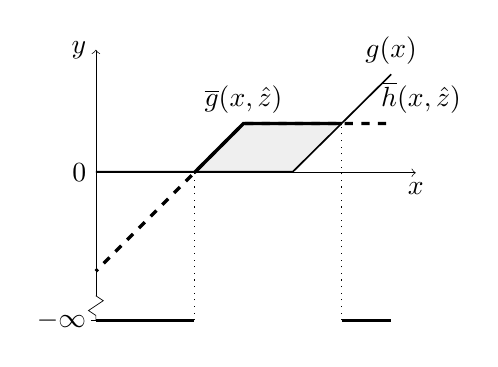
\begin{tikzpicture}[scale=1.25]
        \fill[opacity=0.25, fill=lightgray] (1,0) -- (1.5,0.5) -- (2.5,0.5) -- (2,0) -- cycle;

        \draw [->, line width=0.25] (0,0) -- (3.25,0);
        \draw [->, line width=0.25] (0,-1.25) -- (0,1.25);
        \node[left] at (0,1.25) {$y$};
        \node[below] at (3.25,0) {$x$};
        % \node[anchor=west] at (0.25,1.5) {$\hat{z} = \left(\frac{1}{2},\frac{1}{2}\right)$};
        \node[left] at (0, 0) {$0$};
        \coordinate (P1) at (0,0.01);
        \coordinate (P2) at (2,0.01);
        \coordinate (P3) at (3,1);

        \draw[semithick] (P1) -- (P2) -- (P3);

        % g(x,z)
        \draw[very thick] (1,0) -- (1.5,0.5) -- (2.5,0.5);
        \draw[very thick] (0,-1.5) -- (1,-1.5);
        \draw[very thick] (2.5,-1.5) -- (3,-1.5);
        \draw[dotted] (1,-1.5) -- (1,0);
        \draw[dotted] (2.5,-1.5) -- (2.5,0.5);

        % h(x,z)
        \draw[very thick,dashed,dash phase=2pt] (0,-1) -- (1.5,0.5) -- (3,0.5);

        % discontinuity
        \draw[line width=0.25] (0,-1.25) -- (0.075,-1.3) -- (-0.075,-1.4) -- (0,-1.45) -- (0,-1.5);
        \draw[line width=0.25] (-0.05,-1.5) -- (0,-1.5);
        \node[left] at (0, -1.5) {$-\infty$};

        \node[above] at (1.5,0.5) {$\bar{g}(x, \hat{z})$};
        \node[above right] at (2.8,0.5) {$\bar{h}(x, \hat{z})$};
        
        \node[above] at (3, 1) {\blue{$g(x)$}};
    \end{tikzpicture}
    \caption{Upper bounds $\bar{g}(x,\hat{z})$ and $\bar{h}(x,\hat{z})$ for\\[0.5em] \centering$\blue{g(x) =\!}\displaystyle\max_{x \in [0,2]}\{0, x-2\}$, $\hat{z} = \left(\frac{1}{2},\frac{1}{2}\right)$.}\label{fig:upper_bound_functions_a}
    \end{subfigure} \hspace{2em}
    \begin{subfigure}[t]{0.49\textwidth}
    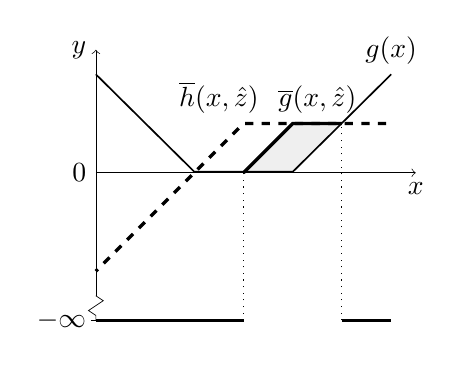
\begin{tikzpicture}[scale=1.25]
        \fill[opacity=0.25, fill=lightgray] (1.5,0) -- (2,0.5) -- (2.5,0.5) -- (2,0) -- cycle;

        \draw [->, line width=0.25] (0,0) -- (3.25,0);
        \draw [->, line width=0.25] (0,-1.25) -- (0,1.25);
        \node[left] at (0,1.25) {$y$};
        \node[below] at (3.25,0) {$x$};
        % \node[anchor=west] at (0.25,1.5) {$\hat{z} = \left(0,\frac{1}{2},\frac{1}{2}\right)$};
        \node[left] at (0, 0) {$0$};
        \coordinate (P1) at (0,1);
        \coordinate (P2) at (1,0.01);
        \coordinate (P3) at (2,0.01);
        \coordinate (P4) at (3,1);

        \draw[semithick] (P1) -- (P2) -- (P3) -- (P4);

        % g(x,z)
        \draw[very thick] (1.5,0) -- (2,0.5) -- (2.5,0.5);
        \draw[very thick] (0,-1.5) -- (1.5,-1.5);
        \draw[very thick] (2.5,-1.5) -- (3,-1.5);
        \draw[dotted] (1.5,-1.5) -- (1.5,0);
        \draw[dotted] (2.5,-1.5) -- (2.5,0.5);

        % h(x,z)
        \draw[very thick, dashed,dash phase=2pt] (0,-1) -- (1.5,0.5) -- (3,0.5);

        % discontinuity
        \draw[line width=0.25] (0,-1.25) -- (0.075,-1.3) -- (-0.075,-1.4) -- (0,-1.45) -- (0,-1.5);
        \draw[line width=0.25] (-0.05,-1.5) -- (0,-1.5);
        \node[left] at (0, -1.5) {$-\infty$};

        \node[above] at (2.25,0.5) {$\bar{g}(x, \hat{z})$};
        \node[above] at (1.25,0.5) {$\bar{h}(x, \hat{z})$};
        
        \node[above] at (3, 1) {\blue{$g(x)$}};
    \end{tikzpicture}
    \caption{Upper bounds $\bar{g}(x,\hat{z})$ and $\bar{h}(x,\hat{z})$ for \\[0.5em] \centering$\blue{g(x) =\!}\displaystyle\max_{x \in [0,2]}\{-x+1, 0, x-2\}$, $\hat{z} = \left(0,\frac{1}{2},\frac{1}{2}\right)$.}\label{fig:upper_bound_functions_b}
    \end{subfigure}\vspace{1em}
    \begin{subfigure}[t]{0.44\textwidth}
    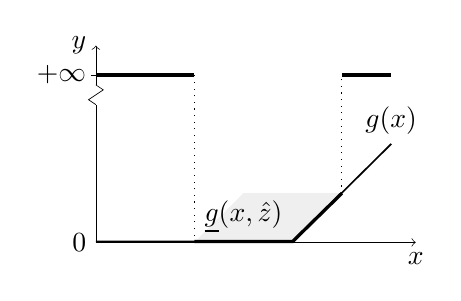
\begin{tikzpicture}[scale=1.25]
        \fill[opacity=0.25, fill=lightgray] (1,0) -- (1.5,0.5) -- (2.5,0.5) -- (2,0) -- cycle;

        \draw [->, line width=0.25] (0,0) -- (3.25,0);
        \draw [line width=0.25] (0,0) -- (0,1.4);
        \node[left] at (0,2) {$y$};
        \node[below] at (3.25,0) {$x$};
        % \node[anchor=west] at (0.25,1.5) {$\hat{z} = \left(\frac{1}{2},\frac{1}{2}\right)$};
        \node[left] at (0, 0) {$0$};
        \coordinate (P1) at (0,0.01);
        \coordinate (P2) at (2,0.01);
        \coordinate (P3) at (3,1);

        \draw[semithick] (P1) -- (P2) -- (P3);

        % g(x,z)
        \draw[very thick] (1,0.01) -- (2,0.01) -- (2.5,0.5);
        \draw[very thick] (0,1.7) -- (1,1.7);
        \draw[very thick] (2.5,1.7) -- (3,1.7);
        \draw[dotted] (1,0) -- (1,1.7);
        \draw[dotted] (2.5,0.5) -- (2.5,1.7);

        % discontinuity
        \draw[line width=0.25] (0,1.4) -- (-0.075,1.45) -- (0.075,1.55) -- (0,1.6);
        \draw[->,line width=0.25] (0,1.6) -- (0,2);
        \draw[line width=0.25] (-0.05,1.7) -- (0,1.7);
        \node[left] at (0, 1.7) {$+\infty$};

        \node[above] at (1.5,0) {$\ubar{g}(x, \hat{z})$};
        
        \node[above] at (3, 1) {\blue{$g(x)$}};
    \end{tikzpicture}
    \caption{Lower bounds $\ubar{g}(x,\hat{z})$ for\\[0.5em] \centering$\blue{g(x) =\!}\displaystyle\max_{x \in [0,2]}\{0, x-2\}$, $\hat{z} = \left(\frac{1}{2},\frac{1}{2}\right)$.}\label{fig:lower_bound_functions_a}
    \end{subfigure} \hspace{2em}
    \begin{subfigure}[t]{0.49\textwidth}
    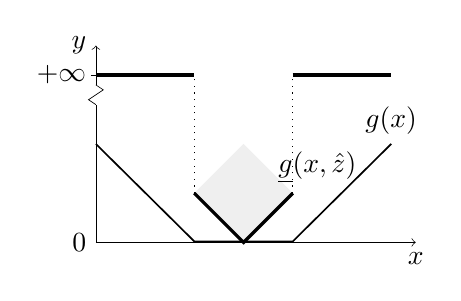
\begin{tikzpicture}[scale=1.25]
        \fill[opacity=0.25, fill=lightgray] (1,0.5) -- (1.5,0) -- (2,0.5) -- (1.5,1) -- cycle;

        \draw [->, line width=0.25] (0,0) -- (3.25,0);
        \draw [line width=0.25] (0,0) -- (0,1.4);
        \node[left] at (0,2) {$y$};
        \node[below] at (3.25,0) {$x$};
        % \node[anchor=west] at (0.25,1.5) {$\hat{z} = \left(0,\frac{1}{2},\frac{1}{2}\right)$};
        \node[left] at (0, 0) {$0$};
        \coordinate (P1) at (0,1);
        \coordinate (P2) at (1,0.01);
        \coordinate (P3) at (2,0.01);
        \coordinate (P4) at (3,1);

        \draw[semithick] (P1) -- (P2) -- (P3) -- (P4);

        % g(x,z)
        \draw[very thick] (1,0.5) -- (1.5,0) -- (2,0.5);
        \draw[very thick] (0,1.7) -- (1,1.7);
        \draw[very thick] (2,1.7) -- (3,1.7);
        \draw[dotted] (1,0.5) -- (1,1.7);
        \draw[dotted] (2,0.5) -- (2,1.7);

        % discontinuity
        \draw[line width=0.25] (0,1.4) -- (-0.075,1.45) -- (0.075,1.55) -- (0,1.6);
        \draw[->,line width=0.25] (0,1.6) -- (0,2);
        \draw[line width=0.25] (-0.05,1.7) -- (0,1.7);
        \node[left] at (0, 1.7) {$+\infty$};

        \node[above] at (2.25,0.5) {$\ubar{g}(x, \hat{z})$};
        
        \node[above] at (3, 1) {\blue{$g(x)$}};
    \end{tikzpicture}
    \caption{Lower bounds $\ubar{g}(x,\hat{z})$ for\\[0.5em] \centering$\blue{g(x) =\!}\displaystyle\max_{x \in [0,2]}\{-x+1, 0, x-2\}$, $\hat{z} = \left(\frac{1}{2},0,\frac{1}{2}\right)$.}\label{fig:lower_bound_functions_b}
    \end{subfigure}
        \caption{Examples of the functions $\bar{g}(x,z)$, $\bar{h}(x,z)$, and $\ubar{g}(x,z)$ defined in~\eqref{eqn:max_ideal_set_primal} and~\eqref{eqn:max_sharp_set_primal} with some fixed value for $z$. \blue{Here, $g(x)$ is the ``maximum'' function of interest, defined below each subfigure. Figures (a) and (c) depict the case $d = 2$ (maximum of two affine functions), while (b) and (d) illustrate when $d = 3$, each pair emphasizing upper and lower bounds respectively.} Note that $\bar{g}(x,z)$ and $\bar{h}(x,z)$ coincide in (a) for $x \in [1,2.5]$, and in (b) for $x \in [2,2.5]$. The thick solid lines represent $\bar{g}(x,z)$ in (a--b) and $\ubar{g}(x,z)$ in (c--d), whereas the dashed lines correspond to $\bar{h}(x,z)$. The thin solid lines represent $\Smax$ and the shaded region is the slice of $\Rcayley$ with $z=\hat{z}$.}
    \label{fig:upper_bound_functions}
\end{figure}

Figure~\ref{fig:upper_bound_functions} depicts slices of the functions $\bar{g}(x,z)$, $\ubar{g}(x,z)$, and $\bar{h}(x,z)$, created by fixing some value of $z$ and varying $x$. Observe that $\bar{g}(x,z)$ can be viewed as the largest value for $y$ such that $(x,y)$ can be written as a convex combination of points in the graph using convex multipliers $z$. Likewise, $\ubar{g}(x,z)$ can be interpreted as the minimum value for $y$. In $\bar{h}(x,z)$, we relax $D_{|k}$ to $D$, and thus we can interpret it similarly to $\bar{g}(x,z)$, except that we may take convex combinations of points constructed by evaluating the affine functions at any point in the domain, not only those where the given function attains the maximum.  Figure~\ref{fig:upper_bound_functions_b} shows that, in general, $\bar{h}(x,z)$ can be strictly looser than $\bar{g}(x,z)$ for $(x,z) \in \Proj_{x,z}(\Rcayley)$. A similar situation occurs for the lower envelopes as illustrated by Figure~\ref{fig:lower_bound_functions_b}. However, we prove in the next section that this does not occur for $d = 2$, along with other desirable properties in special cases.% --- end section-3.tex ---
% --- begin section-4.tex ---
\section{Simplifications to our machinery under common special cases} \label{sec:simplifications}

In this section we study how our dual characterizations in Propositions~\ref{prop:max_ideal_set_dual} and \ref{prop:max_sharp_set_dual} simplify under common special cases with the number of input affine functions $d$ and the input domain $D$.

\subsection{Simplifications when $d=2$} \label{sec:d-2}

% When the set $\Smax$ being formulated consists of taking the maximum of only two affine functions (i.e. $d=2$), we can prove two important additional results: 1) $\Rsharp$ is polyhedral, and 2) it yields a MIP formulation which is not only sharp, but also ideal.
When we consider taking the maximum of only two affine functions (i.e. $d=2$), we can prove that $\Rsharp$ is, in fact, ideal.

We start by returning to Proposition~\ref{prop:max_ideal_set_primal} and show that it can be greatly simplified when $d = 2$. We first show $\ubar{g}(x,z)$ can be replaced by the maximum of the affine functions as illustrated in Figure~\ref{fig:lower_bound_functions_a}, although it is not possible for $d > 2$ as seen in Figure~\ref{fig:lower_bound_functions_b}.

\begin{lemma}\label{lem:max_2_ideal_lb}
    If $d=2$, then at any values of $(x,z)$ where $\bar{g}(x,z)\ge\ubar{g}(x,z)$ (i.e. there exists a $y$ such that $(x,y,z) \in \Rcayley$), we have
    \begin{align*}
        \ubar{g}(x,z) = \max\{w^1 \cdot x + b^1, w^2 \cdot x + b^2\}.
    \end{align*}
\end{lemma}
\begin{proof}
For convenience, we work with the change of variables $x^k \leftarrow \frac{\tx^k}{z_k}$ for each $k \in \llbracket 2 \rrbracket$. Suppose without loss of generality that $x\in D_{|2}$, and consider any feasible solution $(x^1,x^2)$ to the optimization problem for $\ubar{g}(x,z)$, which is feasible by the assumption that $(x,z) \in \Proj_{x,z}(\Rcayley)$. We will show that $(w^1\cdot x^1+b^1)z_1+(w^2\cdot x^2+b^2)z_2\ge w^2\cdot x+b^2$. We assume that $z_2>0$, since otherwise $x=x^1\in D_{|1}\cap D_{|2}$ and the result is immediate.

Since $x=x^1z_1+x^2z_2$ and $z \in \Delta^2$, the line segment joining $x^1$ to $x^2$ contains $x$. Furthermore, since $x^1\in D_{|1}$ and $x^2\in D_{|2}$, this line segment also intersects the hyperplane $\Set{\hat{x}\in\mathbb{R}^\eta | w^1 \cdot \hat{x}+b^1=w^2 \cdot \hat{x}+b^2}$. Let $\hat{x}^1$ denote this point of intersection, and let $\hat{z}^1\in \Delta^2$ be such that $\hat{x}^1=x^1\hat{z}^1_1+x^2\hat{z}^1_2$. Since $x\in D_{|2}$, we know that $\hat{x}^1$ is closer to $x^1$ than $x$, i.e.\ $\hat{z}^1_1 \ge z_1$. Moreover, take the point $\hat{x}^2$ on this line segment such that $x=\hat{x}^1z_1+\hat{x}^2z_2$,
where $\hat{x}^2=x^1\hat{z}^2_1+x^2\hat{z}^2_2$ for some $\hat{z}^2 \in \Delta^2$. We have $\hat{z}^2_1 \le z_1$ since $\hat{x}^2$ is further away from $x^1$ than $x$.  Note that $\hat{x}^1\in D_{|1}\cap D_{|2}$ while $\hat{x}^2\in D_{|2}$, and thus $(\hat{x}^1, \hat{x}^2)$ is feasible.

It can be computed that $\hat{z}^2_1 = z_1\cdot\frac{\hat{z}^1_2}{z_2}$, which implies that $z_1=z_1(\hat{z}^1_1+\hat{z}^1_2)=z_1\hat{z}^1_1+z_2\hat{z}^2_1$ and $z_2=z_2(\hat{z}^2_1+\hat{z}^2_2)=z_1\hat{z}^1_2+z_2\hat{z}^2_2$. Using these two identities, we obtain
\begin{align*}
(w^1\cdot x^1+b^1)z_1+(w^2\cdot x^2+b^2)z_2 
= &\ (w^1\cdot x^1+b^1)(z_1\hat{z}^1_1+z_2\hat{z}^2_1)+(w^2\cdot x^2+b^2)(z_1\hat{z}^1_2+z_2\hat{z}^2_2) \\
= &\ ((w^1\cdot x^1+b^1)\hat{z}^1_1+(w^2\cdot x^2+b^2)\hat{z}^1_2)z_1 \\
& + ((w^1\cdot x^1+b^1)\hat{z}^2_1+(w^2\cdot x^2+b^2)\hat{z}^2_2)z_2 \\
= &\ (f(x^1)\hat{z}^1_1+f(x^2)\hat{z}^1_2)z_1+(f(x^1)\hat{z}^2_1+f(x^2)\hat{z}^2_2)z_2,
\end{align*}
where we let $f(\hat{x})$ denote the function $\max\{w^1\cdot\hat{x}+b^1,w^2\cdot\hat{x}+b^2\}$, recalling that $x^1\in D_{|1}$ and $x^2\in D_{|2}$.  Since $f(\hat{x})$ is convex, by Jensen's inequality the preceding expression is at least
$f(x^1\hat{z}^1_1+x^2\hat{z}^1_2)z_1+f(x^1\hat{z}^2_1+x^2\hat{z}^2_2)z_2$. The preceding expression equals $(w^2\cdot\hat{x}^1+b^2)z_1+(w^2\cdot\hat{x}^2+b^2)z_2$ by the definitions of $\hat{x}^1$ and $\hat{x}^2$, and the fact that they both lie in $D_{|2}$. Recalling the equation $x=\hat{x}^1z_1+\hat{x}^2z_2$ used to select $\hat{x}^2$ completes the proof.
\qed\end{proof}


Moreover, we show that when $d=2$ we can replace $\bar{g}$ with $\bar{h}$, as illustrated in Figure~\ref{fig:upper_bound_functions_a}. This property may not hold when $d > 2$ as shown in Figure~\ref{fig:upper_bound_functions_b}.

\begin{lemma}\label{lem:max_2_ideal_ub}
    If $d = 2$, then at any values of $(x,z)$ where $\bar{g}(x,z)\ge\ubar{g}(x,z)$ (i.e. there exists a $y$ such that $(x,y,z) \in \Rcayley$), we have
\begin{align}\label{eqn:max_2_ideal_ub}
% \bar{g}(x,z) = \max_{\tx^1, \tx^2}\left\{(w^1 \cdot \tx^1 + b^1) (1-z) + (w^2 \cdot \tx^2 + b^2) z : \tx^1 (1-z) + \tx^2 z = x,\ \tx^1 \in D,\ \tx^2 \in D\right\}    
\bar{g}(x,z) = \max_{\tx^1, \tx^2}\Set{w^1 \cdot \tx^1 + b^1 z_1 + w^2 \cdot \tx^2 + b^2 z_2 | \begin{array}{l} x = \tx^1 + \tx^2 \\ \tx^1 \in z_1 \cdot D \\ \tx^2 \in z_2 \cdot D \end{array}}.
\end{align}
\end{lemma}

\begin{proof}

We show that despite expanding the feasible set of the optimization problem in~\eqref{eqn:max_2_ideal_ub} by replacing $D_{|k}$ by $D$, its optimal value is no greater when $(x,z)$ is such that $\bar{g}(x,z)\ge\ubar{g}(x,z)$.  It suffices to show without loss of generality that $w^1 \cdot \tx^1 + b^1 z_1 \geq w^2 \cdot \tx^1 + b^2 z_1$ holds for any optimal $\tx^1, \tx^2$. By the assumption on $(x,z)$ and Lemma~\ref{lem:max_2_ideal_lb}, we have $\bar{g}(x,z) \geq w^2 \cdot x + b^2$, which implies the existence of some optimal $\tx^1, \tx^2$. That is, we have $w^2 \cdot (x - \tx^1) + b^2 z_2 + w^1 \cdot \tx^1 + b^1 z_1 \geq w^2 \cdot x + b^2$, which is equivalent to $w^1 \cdot \tx^1 + b^1 z_1 \geq w^2 \cdot \tx^1 + b^2 z_1$.
% We use the constraint $y \geq w^2 \cdot x + b^2$ implied by Lemma~\ref{lem:max_2_ideal_lb}. Combining this with the constraint $y \leq \bar{g}(x,z)$, which implies the existence of some optimal $\tx^1, \tx^2$, we have $w^2 \cdot (x - \tx^1) + b^2 z_2 + w^1 \cdot \tx^1 + b^1 z_1 \geq w^2 \cdot x + b^2$, which is equivalent to $w^1 \cdot \tx^1 + b^1 z_1 \geq w^2 \cdot \tx^1 + b^2 z_1$.
\qed\end{proof}

After observing that these simplifications are identical to those presented in Proposition~\ref{prop:max_sharp_set_dual}, we obtain the following corollary promised at the beginning of the section.

\begin{corollary} \label{cor:max_2_ideal_general}
    When $d=2$, $\Set{(x,y,z) \in \Rsharp | z \in \{0,1\}^d}$ is an ideal MIP formulation of $\Smax$.
    % When $d=2$, $\Rsharp$ is:
    % \begin{itemize}
    %     \item polyhedral.
    %     \item an ideal MIP formulation for $\Smax$.
    % \end{itemize}
\end{corollary}
\proof{}
Lemmas~\ref{lem:max_2_ideal_lb} and \ref{lem:max_2_ideal_ub} imply that $\Rsharp = \Rideal$, while Proposition~\ref{prop:max_ideal_set_primal} implies that $\Rideal = \Rcayley$, completing the chain and giving the result.
\qed\endproof

% \begin{corollary}\label{cor:max_2_ideal_general}
%     $\Rsharp$ is an ideal formulation
% When $d=2$, $\Rsharp = \Rcayley$.
% % The formulation~\eqref{eqn:max_sharp_set_dual} is ideal when $d = 2$.
% \end{corollary}

In later sections, we will study conditions under which we can produce an explicit inequality description for $\Rsharp$.

% \begin{proof}
%     Identical to proof for Proposition~\ref{prop:max_sharp_set_dual}, except that when $d = 2$ the set $\Ssharp$ from Lemma~\ref{lem:max_sharp_set_primal} is equal to $\text{proj}_{x,y,z}(\Sdisj)$ due to .
    
% \TODO{This is starting to become a maze of lemmas. I'll gladly take ideas to simplify this...}

% \magenta{
% By Lemma~\ref{lem:max_2_ideal_lb},
% the lower-bound constraint~(\ref{eqn:max_ideal_set_primal-2}) for $\Sideal$ is equivalent to the lower-bound constraint~(\ref{eqn:max_sharp_set_primal-2}) for $\Ssharp$ when $d=2$.
% By Lemma~\ref{lem:max_2_ideal_ub}, at all feasible values of $x$ and $z$,
% the upper-bound constraint~(\ref{eqn:max_ideal_set_primal-1}) for $\Sideal$ is equivalent to the upper-bound constraint (\ref{eqn:max_sharp_set_primal-1}) for $\Ssharp$ when $d=2$.
% Therefore, the sets $\Sideal$ and $\Ssharp$ are identical when $d=2$.

% Meanwhile, the set described by constraints~(\ref{eqn:max_sharp_set_dual}) in Proposition~\ref{prop:max_sharp_set_dual} equals $\Ssharp$.  Since this equals $\Sideal$ when $d=2$, the formulation is ideal.
% }
% \qed\end{proof}

\subsection{Simplifications when $D$ is the product of simplices} \label{sec:product-of-simplices}

In this section, we consider another important special case: when the input domain is the Cartesian product of simplices. Indeed, the box domain case introduced in Section~\ref{sec:relu} can be viewed as a product of two-dimensional simplices, and we will also see in Section~\ref{ssec:one-hot-encoding} that this structure naturally arises in machine learning settings with categorical or discrete features.

When $D$ is the product of simplices, we can derive a finite representation for the the set \eqref{eqn:max_sharp_set_dual} (i.e. a finite representation for the infinite family of linear inequalities \eqref{eqn:max_sharp_set_dual-1}) through an elegant connection with the transportation problem. To do so, we introduce the following notation.
\begin{definition} \label{defn:prodSimpl}
Suppose the input domain is $D = \prod_{i=1}^\tau \Delta^{p_i}$, with $p_1+\cdots+p_{\tau}=\eta$. For notational simplicity, we re-organize the indices of $x$ and refer to its entries via $x_{i,j}$, where $i\in\llbracket\tau\rrbracket$ is the simplex index, and $j\in\llbracket p_i\rrbracket$ refers to the coordinate within simplex $i$.
The domain for $x$ is then
\begin{align} \label{eqn:simplexDef}
% D=\Set{ x_{:,:} | x_{i,:} \in \Delta^{p_i} \quad \forall i \in \llbracket \tau \rrbracket },
D=\Set{ ((x_{i,j})_{j=1}^{p_i})_{i=1}^{\tau} | (x_{i,j})_{j=1}^{p_i} \in \Delta^{p_i} \quad \forall i \in \llbracket \tau \rrbracket },
% \begin{array}{cl} \sum_{j=1}^{p_i}x_{ij}=1 & \forall\ i \\ x_{ij}\ge0 & \forall\ i,j \end{array} },
\end{align}
where the rows of $x$ correspond to each simplex. Correspondingly, we re-index the weights of the affine functions so that for each $k\in\llbracket d\rrbracket$, we have
$f^k(x)=\sum_{i=1}^{\tau}\sum_{j=1}^{p_i}w^k_{i,j}x_{i,j}+b^k$.
\end{definition}

Using the notation from Definition~\ref{defn:prodSimpl}, constraints~(\ref{eqn:max_sharp_set_dual-1}) can be written as
\begin{align*}
y\leq\sum_{i=1}^{\tau}\sum_{j=1}^{p_i}\alpha_{i,j}x_{i,j} + \sum_{k=1}^d \left(\max_{x^k \in D}\sum_{i=1}^{\tau}\sum_{j=1}^{p_i}(w^k_{i,j} - \alpha_{i,j})x^k_{i,j} + b^k\right)z_k\quad\forall\alpha\in\mathbb{R}^{\eta}.
\end{align*}
Since $D$ is a product of simplices, the maximization over $x^k\in D$ appearing in the right-hand side above is separable over each simplex $i \in \llbracket \tau \rrbracket$. Moreover, for each simplex $i$, the maximum value of $\sum_{j=1}^{p_i}(w^k_{ij} - \alpha_{ij})x^k_{ij}$, subject to the constraint $x^k \in D$, is obtained when $x^k_{ij}=1$ for some $j\in\llbracket p_i\rrbracket$.
Therefore, the family of constraints~(\ref{eqn:max_sharp_set_dual-1}) is equivalent to
\begin{align}
y &\leq\min_{\alpha}\left(\sum_{i=1}^{\tau}\sum_{j=1}^{p_i}\alpha_{i,j}x_{i,j} + \sum_{k=1}^d \left(\sum_{i=1}^{\tau}\max_{j=1}^{p_i}(w^k_{i,j} - \alpha_{i,j}) + b^k\right)z_k\right) \nonumber \\
&=\sum_{i=1}^{\tau}\min_{\alpha_{i,1},\ldots,\alpha_{i,p_i}}\left(\sum_{j=1}^{p_i}\alpha_{i,j}x_{i,j} + \sum_{k=1}^dz_k\cdot\max_{j=1}^{p_i}(w^k_{i,j} - \alpha_{i,j})\right)+\sum_{k=1}^db^kz_k. \label{eqn:sharp_dual_prod_simpl}
\end{align}

We show that the minimization problem in (\ref{eqn:sharp_dual_prod_simpl}), for any $i$, is equivalent to a transportation problem defined as follows.
\begin{definition} \label{def:trans}
For any values $x \in \Delta^p$ and $z \in \Delta^d$, and arbitrary weights $w^k_j\in\mathbb{R}$ for all $j\in\llbracket p\rrbracket$ and $k\in\llbracket d \rrbracket$, define the \textit{max-weight transportation problem} to be
\begin{alignat*}{2}
% \trans((w^k_j)_{j=1,k=1}^{p,d},(x_j)_{j=1}^p,(z_k)_{k=1}^d) \defeq \max_{\beta}\quad&\sum_{k=1}^d\sum_{j=1}^pw^k_j\beta^k_j \\
% \trans(x,z;w^1,\ldots,w^d) \defeq \max_{\beta \geq 0}\quad&\sum_{k=1}^d\sum_{j=1}^pw^k_j\beta^k_j \\
% \operatorname{s.t.}\quad&\sum_{k=1}^d\beta^k_j =x_j \quad&\forall j\in\llbracket p\rrbracket \\
% &\sum_{j=1}^p\beta^k_j =z_k \quad&\forall k\in\llbracket d\rrbracket
\trans(x,z;w^1,\ldots,w^d) \defeq \max_{\beta \geq 0}\Set{\sum_{k=1}^d\sum_{j=1}^pw^k_j\beta^k_j \;|\; \begin{alignedat}{3}\sum_{k=1}^d\beta^k_j &=x_j \quad\forall j\in\llbracket p\rrbracket \\
\sum_{j=1}^p\beta^k_j &=z_k \quad\forall k\in\llbracket d\rrbracket\end{alignedat}}
% &\beta^k_j \ge0 \quad&\forall j\in\llbracket p\rrbracket,k\in\llbracket d\rrbracket
\end{alignat*}
% Let $\trans((w^k_j)_{j=1,k=1}^{p,d},(x_j)_{j=1}^p,(z_k)_{k=1}^d)$ denote the optimal objective value of this LP.
\end{definition}
In the transportation problem, since $\sum_jx_j=1=\sum_kz_k$, it follows that $\beta^k_j \in [0,1]$, and so this value can be interpreted as the percent of total flow ``shipped" between $j$ and $k$.
The relation to~(\ref{eqn:sharp_dual_prod_simpl}) is now established through LP duality.

\begin{proposition} \label{prop:transportationDuality}
For any fixed $x \in \Delta^{p}$ and $z \in \Delta^d$,
\begin{align} \label{eqn:suppress_i}
    \min_{\alpha} \left( \sum_{j=1}^{p}\alpha_{j}x_{j} + \sum_{k=1}^dz_k\cdot\max_{j=1}^p(w^k_{j} - \alpha_{j}) \right) = \trans(x,z;w^1,\ldots,w^d).
\end{align}
% the minimum value of $\left(\sum_{j=1}^{p_i}\alpha_{ij}x_{ij} + \sum_{k=1}^dz_k\cdot\max_{j=1,\ldots,p_i}(w^k_{ij} - \alpha_{ij})\right)$ over $\alpha_{i1},\ldots,\alpha_{ip_i}\in\mathbb{R}$ equals $\trans((w^k_{ij})_{j=1,k=1}^{p,d},(x_{ij})_{j=1}^p,(z_k)_{k=1}^d)$.
Therefore, when $D$ is a product of simplices, the constraints \eqref{eqn:max_sharp_set_dual-1} can be replaced in \eqref{eqn:max_sharp_set_dual} with the single inequality
\begin{align} \label{eqn:unsupress_i}
% y\le\sum_{i=1}^{\tau}\trans((w^k_{ij})_{j=1,k=1}^{p,d},(x_{ij})_{j=1}^p,(z_k)_{k=1}^d)+\sum_{k=1}^db^kz_k.
y\le\sum_{i=1}^{\tau}\trans((x_{i,j})_{j=1}^{p_i},z;(w^1_{i,j})_{j=1}^{p_i},\ldots,(w^d_{i,j})_{j=1}^{p_i})+\sum_{k=1}^db^kz_k.
% y\le\sum_{i=1}^{\tau}\trans(x_{i,:},z;w^1_{i,:},\ldots,w^d_{i,:})+\sum_{k=1}^db^kz_k.
\end{align}
\end{proposition}

\begin{proof}
By using a variable $\gamma_{k}$ to model the value of $\max_{j=1}^{p}(w^k_{j} - \alpha_{j})$ for each $k\in\llbracket d\rrbracket$, the minimization problem on the LHS of~\eqref{eqn:suppress_i} is equivalent to
\begin{alignat*}{2}
\min_{\alpha,\gamma}\Set{\sum_{j=1}^{p}\alpha_{j}x_{j}+\sum_{k=1}^d\gamma_{k}z_k \;|\;
\gamma_{k} \ge w^k_{j}-\alpha_{j} \quad\forall k\in\llbracket d\rrbracket,j\in\llbracket p\rrbracket}
\end{alignat*}
which is a minimization LP with free variables $\alpha_j$ and $\gamma_k$.
Applying LP duality, this completes the proof of equation~\eqref{eqn:suppress_i}. The inequality
\eqref{eqn:unsupress_i} then arises by substituting equation~\eqref{eqn:suppress_i} into~\eqref{eqn:sharp_dual_prod_simpl}, for every simplex $i=1,\ldots,\tau$.
\qed\end{proof}

\subsection{Simplifications when both $d=2$ and $D$ is the product of simplices} \label{sec:d-2-product-of-simplices}

%This is a general result that can leverage any fast methods for solving transportation problems.
Proposition~\ref{prop:transportationDuality} shows that, when the input domain is a product of simplices, the tightest upper bound on $y$ can be computed through a series of transportation problems. We now leverage the fact that if either side of the transportation problem from Definition~\ref{def:trans} (i.e. $p$ or $d$) has only two entities, then it reduces to a simpler fractional knapsack problem.
Later, this will allow us to represent \eqref{eqn:sharp_dual_prod_simpl}, in either of the cases $d=2$ or $p_1=\cdots=p_{\tau}=2$, using an explicit finite family of linear inequalities in $x$ and $z$ which has a greedy linear-time separation oracle.
\begin{proposition} \label{prop:simplicesD2Explicit}
Given data $w^1, w^2 \in \bbR^p$, take $\tw_j = w^1_j-w^2_j$ for all $j\in\llbracket p\rrbracket$, and suppose the indices have been sorted so that
$\tw_1\le\cdots\le\tw_p$.
Then
\begin{align} \label{eqn:trans-is-fractional-knapsack}
% \trans((w^k_j)_{j=1,k=1}^{p,2},(x_j)_{j=1}^p,(z_k)_{k=1}^2)=\min_{J=1,\ldots,p}\left(\tw_Jz_1+\sum_{j=J+1}^{p}(\tw_j-\tw_J)x_j\right)+\sum_{j=1}^{p}w^2_jx_j.
\trans(x,z;w^1,w^2)=\min_{J=1}^{p}\left(\tw_Jz_1+\sum_{j=J+1}^{p}(\tw_j-\tw_J)x_j\right)+\sum_{j=1}^{p}w^2_jx_j.
\end{align}
Moreover, a $J \in \llbracket p \rrbracket$ that attains the minimum in the right-hand side of \eqref{eqn:trans-is-fractional-knapsack} can be found in $\mathcal{O}(p)$ time.
% Moreover, the $J\in\llbracket p\rrbracket$ minimizing the RHS can be found in $\mathcal{O}(p)$ time (whereas the naive runtime would be $\mathcal{O}(p^2)$ because the inner sum is linear in $p$).
\end{proposition}

\begin{proof}
When $d=2$, the transportation problem becomes
\begin{alignat}{2} \label{eqn:trans-opt-proof}
\max_{\beta^1,\beta^2 \geq 0}\Set{\sum_{j=1}^p(w^1_j\beta^1_j+w^2_j\beta^2_j)\;|\;\beta^1_j+\beta^2_j =x_j \quad\forall j\in\llbracket p\rrbracket,\quad \sum_{j=1}^p\beta^1_j =z_1}
% & \beta^1_j,\beta^2_j \ge0 \quad&\forall j\in\llbracket p\rrbracket,
\end{alignat}
where the constraint $\sum_{j=1}^p\beta^2_j=z_2$ is implied because
% \begin{align*}
$\sum_{j=1}^p\beta^2_j=\sum_{j=1}^p(x_j-\beta^1_j)=1-\sum_{j=1}^p\beta^1_j=1-z_1=z_2$.
% \end{align*}
Substituting $\beta^2_j=x_j-\beta^1_j$ for all $j \in \llbracket p \rrbracket$ and then omitting the superscript ``1'', \eqref{eqn:trans-opt-proof} becomes
\begin{alignat*}{2}
\max_{\beta}\Set{\sum_{j=1}^p(w^1_j-w^2_j)\beta_j+\sum_{j=1}^pw^2_jx_j\;|\;\sum_{j=1}^p\beta_j =z_1,\quad  0\le\beta_j \le x_j \quad \forall j\in\llbracket p\rrbracket}
\end{alignat*}
which is a fractional knapsack problem that can be solved greedily.

An optimal solution to the fractional knapsack LP above, assuming the sorting $w^1_1-w^2_1\le\cdots\le w^1_p-w^2_p$, can be computed greedily. Let $J\in\llbracket p\rrbracket$ be the \textit{maximum} index at which $\sum_{j=J}^px_j\ge z_1$.
We set $\beta_j = 0$ for all $j < J$, $\beta_J = z_1 - \sum_{j=J+1}^p x_j$, and $\beta_j = x_j$ for each $j > J$.
% We set $\beta_j = \begin{cases} 0 & j < J \\ z_1 - \sum_{j=J+1}^p x_j & j = J \\ x_j & j > J \end{cases}$.
% $\beta_j=x_j$ for all $j>J$; $\beta_J=z_1-\sum_{j>J}x_j$; and $\beta_j=0$ for all $j<J$.
The optimal cost is
\begin{align*}
\sum_{j=J+1}^p(w^1_j-w^2_j)x_j+(w^1_J-w^2_J)\left(z_1-\sum_{j=J+1}^px_j\right)+\sum_{j=1}^pw^2_jx_j,
\end{align*}
which yields the desired expression after substituting $\tw_j=w^1_j-w^2_j$ for all $j\ge J$.
Moreover, the index $J$ above can be found in $\mathcal{O}(p)$ time by storing a running total for $\sum_{j=J}^p x_j$, completing the proof.
\qed\end{proof}

Observe that the $\mathcal{O}(p)$ runtime in Proposition~\ref{prop:simplicesD2Explicit} is non-trivial, as a na\"{i}ve implementation would run in time $\mathcal{O}(p^2)$, as the inner sum is linear in $p$.

Combining Propositions \ref{prop:transportationDuality} and \ref{prop:simplicesD2Explicit} immediately yields the following result.
\begin{corollary} \label{cor:simplicesD2Result}
Suppose that $d=2$ and that $D$ is a product of simplices.  Let $z = z_1 \equiv 1-z_2$.
For each simplex $i \in \llbracket \tau \rrbracket$, take $\tw_{i,j} = w^1_{i,j}-w^2_{i,j}$ for all $j=1,\ldots,p_i$ and relabel the indices so that $\tw_{i,1}\le\cdots\le\tw_{i,p_i}$.
Then, in the context of \eqref{eqn:max_sharp_set_dual}, the upper-bound constraints \eqref{eqn:max_sharp_set_dual-1} are equivalent to
\begin{align}
&y\le\sum_{i=1}^{\tau}\left(\tw_{i,J(i)}z+\sum_{j=J(i)+1}^{p_i}(\tw_{i,j}-\tw_{i,J(i)})x_{i,j}+\sum_{j=1}^{p_i}w^2_{i,j}x_{i,j}\right)+(b^1-b^2)z+b^2 \nonumber \\
&\hspace{9em}\forall\text{ mappings $J:\llbracket\tau\rrbracket\to\mathbb{Z}$ with $J(i)\in\llbracket p_i\rrbracket\ \forall i\in\llbracket\tau\rrbracket$.} \label{eqn:simplicesD2upperBound}
\end{align}
Moreover, given any point $(x,y,z)\in D\times\mathbb{R}\times[0,1]$, feasibility can be verified or a most violated constraint can be found in $\mathcal{O}(p_1+\cdots+p_{\tau})$ time.
\end{corollary}
Corollary~\ref{cor:simplicesD2Result} gives an explicit finite family of linear inequalities equivalent to \eqref{eqn:max_sharp_set_dual}. Moreover, we have already shown in Corollary~\ref{cor:max_2_ideal_general} that $\Rsharp$ yields an ideal formulation when $d=2$. Hence, we have an ideal nonextended formulation whose exponentially-many inequalities can be separated in $\mathcal{O}(p_1+\cdots+p_{\tau})$ time, where the initial sorting requires $\mathcal{O}(p_1\log p_1+\cdots+p_{\tau}\log p_{\tau})$ time. Note that this sorting can be avoided: we may instead solve the fractional knapsack problem in the separation via weighted median in $\mathcal{O}(p_1+\cdots+p_{\tau})$ time~\cite[Chapter 17.1]{Korte:2000}.

We can also show that none of the constraints in~\eqref{eqn:simplicesD2upperBound} are redundant.
\begin{proposition} \label{prop:simplicesD2FacetDefining}
Consider the polyhedron $P$ defined as the intersection of all halfspaces corresponding to the inequalities \eqref{eqn:simplicesD2upperBound}. Consider some arbitrary mapping $J : \llbracket \tau \rrbracket \to \bbZ$ with $J(i) \in \llbracket p_i \rrbracket$ for each $i \in \llbracket \tau \rrbracket$. Then the inequality in \eqref{eqn:simplicesD2upperBound} for $J$ is irredundant with respect to $P$. That is, removing the halfspace corresponding to mapping $J$ (note that this halfspace could also correspond to other mappings) from the description of $P$ will strictly enlarge the feasible set.

% None of the constraints in (\ref{eqn:simplicesD2upperBound}) are redundant.
% That is, consider (\ref{eqn:simplicesD2upperBound}) as an intersection of half-spaces, which defines a polyhedron over $(x,y,z)\in D\times\mathbb{R}\times[0,1]$.
%If we remove the half-space corresponding to any mapping $J$ (note that this half-space could correspond to other mappings, too), then the polyhedron is enlarged because the upper bound on $y$ is relaxed.
\end{proposition}
\begin{proof}
Fix a mapping $J$.  Consider the feasible points with $z=1/2$, and $x_{i,j}= \bbone[j = J(i)]$ for each $i$ and $j$.
At such points, the constraint corresponding to any mapping $J' \neq J$ in (\ref{eqn:simplicesD2upperBound}) is
\begin{align*}
y &\le\sum_{i=1}^{\tau}\left(\frac{\tw_{i,J'(i)}}{2}+\sum_{j=J'(i)+1}^{p_i}(\tw_{i,j}-\tw_{i,J'(i)})\mathbb{1}[j=J(i)]+\sum_{j=1}^{p_i}w^2_{i,j}\mathbb{1}[j=J(i)]\right)+\frac{b^1+b^2}{2} \\
&=\sum_{i=1}^{\tau}\left(\frac{\tw_{i,J'(i)}}{2}+(\tw_{i,J(i)}-\tw_{i,J'(i)})\mathbb{1}[J'(i)<J(i)]\right)+\sum_{i=1}^{\tau}w^2_{i,J(i)}+\frac{b^1+b^2}{2}.
\end{align*}
For any simplex $i$, recall that the indices are sorted so that $\tw_{i1}\le\cdots\le\tw_{ip_i}$.
Thus, if $J'(i)\ge J(i)$, then the expression inside the outer parentheses equals $\frac{\tw_{i,J'(i)}}{2} \geq \frac{\tw_{i,J(i)}}{2}$.
On the other hand, if $J'(i)<J(i)$, then the expression inside the outer parentheses can be re-written as $\frac{\tw_{i,J(i)}}{2}+\frac{\tw_{i,J(i)}-\tw_{i,J'(i)}}{2} \geq \frac{\tw_{i,J(i)}}{2}$.
Therefore, setting $J'(i)=J(i)$ for every simplex $i$ achieves the tightest upper bound in (\ref{eqn:simplicesD2upperBound}), which simplifies to
\begin{align} \label{eqn:facetTightestUpperBound}
y\le\sum_{i=1}^{\tau}\frac{\tw_{i,J(i)}}{2}+\sum_{i=1}^{\tau}w^2_{i,J(i)}+\frac{b^1+b^2}{2}.
\end{align}

Now, suppose that the same upper bound on $y$ is achieved by a mapping $J'$ such that $J'(i)\neq J(i)$ on a simplex $i$.
By the argument above, regardless of whether $J'(i)>J(i)$ or $J'(i)<J(i)$, the expression inside the outer parentheses can equal $\frac{\tw_{i,J(i)}}{2}$ only if $\tw_{i,J'(i)}=\tw_{i,J(i)}$.
In this case, inspecting the term inside the summation in \eqref{eqn:simplicesD2upperBound} for mappings $J$ and $J'$, we observe that regardless of the values of $x$ or $z$,
\begin{align*}
\tw_{i,J'(i)}z+\sum_{j=J'(i)+1}^{p_i}(\tw_{i,j}-\tw_{i,J'(i)})x_{i,j}=\tw_{i,J(i)}z+\sum_{j=J(i)+1}^{p_i}(\tw_{i,j}-\tw_{i,J(i)})x_{i,j}.
\end{align*}
Therefore, for a mapping $J'$ to achieve the tightest upper bound~(\ref{eqn:facetTightestUpperBound}), it must be the case that $\tw_{i,J'(i)}=\tw_{i,J(i)}$ on every simplex $i$, and so $J'$ and $J$ necessarily correspond to the same half-space in $D\times\mathbb{R}\times[0,1]$, completing the proof.
\qed\end{proof}

%Note that Proposition~\ref{prop:simplicesD2FacetDefining} does not preclude the possibility that distinct choices for $J$ in \eqref{eqn:simplicesD2upperBound} will correspond to the same halfspace.

To close this section, we consider the setting where every simplex is 2-dimensional, i.e.\ $p_1=\cdots=p_{\tau}=2$, but the number of affine functions $d$ can be arbitrary.
Note that by contrast, the previous results (Proposition~\ref{prop:simplicesD2Explicit}, Corollary~\ref{cor:simplicesD2Result}, Proposition~\ref{prop:simplicesD2FacetDefining}) held in the setting where $d=2$ but $p_1,\ldots,p_{\tau}$ were arbitrary.
We exploit the symmetry of the transportation problem to immediately obtain the following analogous results, all wrapped up into Corollary~\ref{cor:simplicesP2}.

\begin{corollary} \label{cor:simplicesP2}
Given data $w^1, \ldots, w^d \in \bbR^2$, take $\tw^k = w^k_1 - w^k_2$ for all $k\in\llbracket d\rrbracket$, and suppose the indices have been sorted so that
$\tw^1\le\cdots\le\tw^d$.
Then
\begin{align} \label{eqn:p-2-trans-knapsack}
% \trans((w^k_j)_{j=1,k=1}^{2,d},(x_j)_{j=1}^2,(z_k)_{k=1}^d)=\min_{K=1,\ldots,d}\left(\tw^Kx_1+\sum_{k=1}^{K}w^k_2z_k+\sum_{k=K+1}^{d}(w^k_1-\tw^J)z_k\right).
\trans(x,z;w^1,\ldots,w^d)=\min_{K=1}^d\left(\tw^Kx_1+\sum_{k=1}^{K}w^k_2z_k+\sum_{k=K+1}^{d}(w^k_1-\tw^K)z_k\right).
\end{align}
Moreover, a $K \in \llbracket d \rrbracket$ that attains the minimum in the right-hand side of \eqref{eqn:p-2-trans-knapsack} can be found in $\mathcal{O}(d)$ time.

Therefore, suppose that $D$ is a product of $\tau$ simplices of dimensions $p_1=\cdots=p_{\tau}=2$.
For each simplex $i\in\llbracket\tau\rrbracket$, take $\tw^k_i=w^k_{i,1}-w^k_{i,2}$ for all $k=1,\ldots,d$ and relabel the indices so that $\tw^1_i\le\cdots\le\tw^d_i$.
Then, in the context of \eqref{eqn:max_sharp_set_dual}, the upper-bound constraints \eqref{eqn:max_sharp_set_dual-1} are equivalent to
\begin{align}
y &\le\sum_{i=1}^{\tau}\left(\tw^{K(i)}_ix_{i,1}+\sum_{k=1}^{K(i)}w^k_{i,2}z_k+\sum_{k=K(i)+1}^{d}(w^k_{i,1}-\tw^{K(i)}_i)z_k\right)+\sum_{k=1}^db^kz_k \nonumber \\
&\hspace{18em}\forall\text{ mappings $K:\llbracket\tau\rrbracket\to\llbracket d\rrbracket$.} \label{eqn:p-2-trans-knapsack-full}
\end{align}
Furthermore, none of the constraints in~\eqref{eqn:p-2-trans-knapsack-full} are redundant.
\end{corollary}

Corollary~\ref{cor:simplicesP2} will be particularly useful in Section~\ref{ssec:max-cuts}, where it will allow us to derive sharp formulations for the maximum of $d$ affine functions over a box input domain, in analogy to \eqref{eqn:simplicesD2upperBound}.

% Corollary~\ref{cor:simplicesP2} is used to derive a formulation analogous to (\ref{eqn:simplicesD2upperBound}) when we allow the number of affine functions $d$ to be greater than 2, and instead assume that $p_1=\cdots=p_{\tau}=2$ (as is the case when the domain is a box).

% --- end section-4.tex ---
% --- begin section-5.tex ---
\section{Applications of our machinery} \label{sec:applications}

We are now prepared to return to the concrete goal of this paper: building strong MIP formulations for nonlinearities used in modern neural networks.


% \subsection{Practical formulations and cuts for the Max nonlinearity}

% We turn our attention to the regime where $d > 2$, with the goal of producing practically useful (i.e. explicit, finite descriptions of) strong MIP formulations for the maximum of $d$ affine functions.

% \subsubsection{A tight big-M formulation}

% % Separating the inequalities in Lemma~\ref{lem:max_ideal_set_dual} may be expensive for large networks, and thus we consider a subset of those inequalities to either avoid separation or make it faster. However, we still need to ensure that the MIP formulation is valid for $\gr(\Max{} \circ (f^1,\ldots,f^d); D)$. In the following pair of propositions, we present a small subset of these inequalities that ensure validity and are facet-defining. In particular, we select $2d$ inequalities~\eqref{eqn:max_ideal_set_dual-1} and~\eqref{eqn:max_ideal_set_dual-2}: those corresponding to $\bar{\alpha}, \ubar{\alpha} \in \{ w^1, \ldots, w^d \}$. Although we avoid the need for separation, computing the tightest possible coefficients for these constraints may require solving $\mathcal{O}(d^2)$ LPs. Below we write the formulation in terms of general big-M coefficients and we discuss later in this section weaker but more tractable values for these coefficients.

% We start by presenting a tightened big-$M$ formulation for the maximum of $d$ affine functions over an arbitrary polytope input domain. We can view the formulation as a relaxation of the system in Proposition~\ref{prop:max_ideal_set_dual}, where we select $d$ inequalities from each of \eqref{eqn:max_ideal_set_dual-1} and~\eqref{eqn:max_ideal_set_dual-2}: those corresponding to $\bar{\alpha}, \ubar{\alpha} \in \{ w^1, \ldots, w^d \}$. This subset yields a valid formulation, and we obviate the need for direct separation. This formulation can also be viewed as an application of Proposition 6.2 of Vielma~\cite{Vielma:2015}, and is similar to the big-$M$ formulations for generalized disjunctive programs of Trespalacios and Grossmann~\cite{Trespalacios:2014}.

% \begin{proposition}\label{prop:max_big_m}
% Take coefficients $N$ such that, for each $\ell, k \in \llbracket d \rrbracket$ with $\ell \neq k$,
%     \begin{subequations} \label{eqn:optimal-coefficients}
%     \begin{align}
%         N^{\ell,k,+} &\geq \max_{x^k \in D_{|k}}\{(w^k - w^\ell) \cdot x^k\} \label{eqn:optimal-coefficients-1}\\
%         N^{\ell,k,-} &\leq \min_{x^k \in D_{|k}}\{(w^k - w^\ell) \cdot x^k\} ,\label{eqn:optimal-coefficients-2}
%     \end{align}
%     \end{subequations}
% and $N^{k,k,+} = N^{k,k,-} = 0$ for all $k \in \llbracket d \rrbracket$. Then a valid MIP formulation for $\gr(\emph{\Max{}} \circ (f^1,\ldots,f^d); D)$ is:
% \begin{subequations}\label{eqn:max_big_m}
% \begin{align}
%     y \leq w^\ell \cdot x + \sum_{k=1}^d (N^{\ell,k,+} + b^k) z_k&\quad\forall \ell \in \llbracket d \rrbracket\label{eqn:max_big_m-1}\\
%     y \geq w^\ell \cdot x + \sum_{k=1}^d (N^{\ell,k,-} + b^k) z_k&\quad\forall \ell \in \llbracket d \rrbracket\label{eqn:max_big_m-2}\\
%     (x,z) \in D \times \Delta^d \label{eqn:max_big_m-3} \\
%     z \in \{0,1\}^d\label{eqn:max_big_m-4}
% \end{align}
% \end{subequations}
% % Moreover, the inequalities~\eqref{eqn:max_big_m-1} and~\eqref{eqn:max_big_m-2} are facet-defining.
% \end{proposition}
% \begin{proof}
% See Appendix~\ref{app:max_big_m}.
% \qed\end{proof}

% % Under mild conditions, each of the big-$M$ constraints we have selected in \eqref{eqn:max_big_m} are facet-defining.

% % \begin{lemma}
% %     Under the strict activity assumption, each $D_{|k}$ is full-dimensional.
% % \end{lemma}
% % \proof{}
% %     By definition of strict activity, there exists some $x \in D \cap D_{|k}$ such that $f^k(x) > f^\ell(x)$ for each $\ell \neq k$. As each of the $f^\ell$ is linear, there exists some $x^\prime \in \relint(D_{|k})$ in the neighborhood of $x$ with $f^k(x^\prime) > f^\ell(x^\prime)$ for each $\ell \neq k$. The proposed feasible points then take the form $(x^i,y^i) = (x^\prime + \epsilon {\bf e}^i, f^k(x^\prime + \epsilon {\bf e}^i))$ for each $i \in \llbracket \eta \rrbracket$. Along with $(x^\prime,f^k(x^\prime))$, this is $\eta + 1$ affinely independent points
% % \endproof

% % \begin{proposition}\label{prop:max-facets}
% % Presume that each set $D_{|k}$ is nonempty, and take some $\ell \in \llbracket d \rrbracket$. If $D_{|k}$ is full-dimensional (i.e. has dimension $\eta$), then the inequalities~\eqref{eqn:max_big_m-1} and~\eqref{eqn:max_big_m-2} are facet-defining.
% % \end{proposition}

% % \begin{proof}
% % We prove the result for \eqref{eqn:max_big_m-1}; the argument for \eqref{eqn:max_big_m-2} follows in the same manner, merely interchanging an $\arg\max$ for an $\arg\min$ below.

% % Note that, under the nonemptiness assumption, the feasible region for \eqref{eqn:max_big_m} has dimension $\eta+d$. In order to show that the constraint is facet-defining, we identify $\eta+d$ affinely independent feasible points for the MIP that satisfy the given constraint at equality.

% % Fix a point $\hat{x}$ in the interior of $D_{|\ell}$, which exists since $D_{|\ell}$ has dimension $\eta$. Denote the feasible point $p^0 = (\hat{x}, f^\ell(\hat{x}), {\bf e}^\ell)$. Since $\hat{x}$ is in the interior of $D_{|\ell}$, there exists a sufficiently small $\epsilon > 0$ such that the points $p^i = (\hat{x} + \epsilon {\bf e}^i, f^\ell(\hat{x} + \epsilon {\bf e}^i), {\bf e}^\ell)$ are feasible for all $i \in \llbracket \eta \rrbracket$. Note that each of the $\eta+1$ points $p^0, p^1, \ldots, p^\eta$ satisfies the constraint at equality.

% % Now for each $k \in \llbracket d \rrbracket \backslash \{\ell\}$, take the point $\tx^k \in \arg\max_{\tx \in D_{|k}}f^k(\tx)-f^\ell(\tx)$, along with $\tilde{p}^k = (\tx^k, f^k(\tx^k), {\bf e}^k)$. This point $\tilde{p}^k$ is feasible for \eqref{eqn:max_big_m}, and satisfies the given constraint at equality.

% % To finish, we must show that the $\eta + d$ points constructed thus far are affinely independent. Presume w.l.o.g. that $\ell = 1$. The result follows by showing the following matrix has full row rank:
% % \[
% %     \begin{pmatrix} \tilde{p}^2 - p^0 \\ \vdots \\ \tilde{p}^d - p^0 \\ p^1 - p^0 \\ \vdots \\ p^\eta - p^0  \end{pmatrix} = \begin{pmatrix} 
% %         \tx^2 - \hat{x} & f^2(\tx^2) - f^1(\hat{x}) & {\bf e}^2 - {\bf e}^1 \\
% %         \vdots & \vdots & \vdots \\
% %         \tx^d - \hat{x} & f^d(\tx^d) - f^1(\hat{x}) & {\bf e}^d - {\bf e}^1 \\
% %         \epsilon {\bf e}^1 & w_1 \epsilon & 0 \\
% %         \vdots & \vdots & \vdots \\
% %         \epsilon {\bf e}^\eta & w_\eta \epsilon & 0
% %     \end{pmatrix}.
% % \]
% % If we permute the last $d-1$ columns (corresponding to the $z_2$ to $z_d$ variables) to the first $d-1$ columns, we observe that the resulting matrix is upper triangular with a nonzero diagonal, and so has full row rank. Therefore, the starting matrix also has full row rank, as we only applied elementary row operations, and therefore the $\eta+d$ points are affinely independent, giving the result. 

% % \qed\end{proof}


% There are number of observations to be made about the formulation \eqref{eqn:max_big_m}.

% First, the coefficients $N^{\ell,k,+}$ and and $N^{\ell,k,-}$ are the ``big-$M$ coefficients'' that would need to be computed to construct a standard big-$M$ formulation, modulo the constant offset terms $b^k$.

% Second, the tightest possible coefficients in \eqref{eqn:optimal-coefficients} can be computed exactly by solving an LP for each pair of input affine functions $\ell \neq k$. While this might be exceedingly computationally expensive if $d$ is large, it is potentially viable if $d$ is a small fixed constant. For example, the max pooling neuron computes the maximum over a rectangular window in a larger array~\cite[Section 9.3]{Goodfellow:2016}, and is frequently used in image classification architectures. Typically, max pooling units work with a $2 \times 2$ or a $3 \times 3$ window, in which case $d=4$ or $d=9$, respectively.

% Third, if in practice we observe that if the set $D_{|k}$ is empty, then we can infer that the neuron is not irreducible as the $k$-th input function is never the maximum, and we can safely prune it. In particular, if we attempt to compute the coefficients for $z_k$ and it is proven infeasible, we can prune the $k$-th function.

% Fourth, in the case where $D = [L,U]$ and $d$ is sufficiently large that we cannot tractably compute the tightest coefficients in \eqref{eqn:optimal-coefficients}, we can readily produce valid coefficients by relaxing the constraint $\tx \in D_{|\ell}$ to $\tx \in [L,U]$. We can then compute the corresponding values by inspecting the values of the input functions at the corners of the domain $[L,U]$:
% \begin{subequations} \label{eqn:corner-coefficients}
% \begin{align}
%     N^{\ell,k,+} &= \sum_{i=1}^\eta \max\{(w^k_i-w^\ell_i)L_i, (w^k_i-w^\ell_i)U_i)\} \\
%     N^{\ell,k,-} &= \sum_{i=1}^\eta \min\{(w^k_i-w^\ell_i)L_i, (w^k_i-w^\ell_i)U_i)\}
% \end{align}
% \end{subequations}
% for each $\ell \neq k$. All coefficients for formulation \eqref{eqn:max_big_m} can then be computed in time $\mathcal{O}(d^2 \cdot \eta)$. Although potentially suboptimal, they may still lead to a big-$M$ formulation that is substantially stronger than those in the literature. For example, the tightest version of the formulation of Tjeng et al.~\cite{Tjeng:2017} is equivalent in our framework to selecting for each $\ell \neq k$:
% \begin{subequations} \label{eqn:vincent-coefficients}
% \begin{align*}
%     N^{\ell,k,+} &= b^\ell - b^k + \max\limits_{t \neq \ell} \left( \max\limits_{\tx \in [L,U]} w^t \cdot \tx - \min\limits_{\mathring{x} \in [L,U]} w^\ell \cdot \mathring{x} \right)\\
%     N^{\ell,k,-} &= b^\ell - b^k.
% \end{align*}
% \end{subequations}
% Note in particular that as the inner maximization and minimization are completely decoupled, and that the outer maximization in the definition of $N^{\ell,k,+}$ is completely independent of $k$.

% % Finally, the formulation~\eqref{eqn:max_big_m} can be generalized for arbitrary functions $f^i$ by respectively expressing~\eqref{eqn:max_big_m-1} and~\eqref{eqn:max_big_m-2} as
% % \begin{align*}
% %     y \leq f^\ell(x) + \sum_{k=1}^d \max_{\tx \in D_{|k}} (f^k(\tx) - f^\ell(\tx)) z_k\quad\forall \ell \in \llbracket d \rrbracket,\\
% %     y \geq f^\ell(x) + \sum_{k=1}^d \min_{\tx \in D_{|k}} (f^k(\tx) - f^\ell(\tx)) z_k\quad\forall \ell \in \llbracket d \rrbracket.
% % \end{align*}
% % However, we must of course restrict $f^i$ to be affine functions if we would like an LP relaxation.


\subsection{A hereditarily sharp formulation for \Max{} on box domains} \label{ssec:max-cuts}

We can now present a hereditarily sharp formulation, with exponentially-many constraints that can be efficiently separated, for the maximum of $d > 2$ affine functions over a shared box input domain. % This result follows from a variable transformation of Corollary~\ref{cor:simplicesP2}; see Appendix~\ref{app:max_sharp} for a detailed proof.
\begin{proposition}\label{prop:max_sharp}
    For each $k, \ell \in \llbracket d \rrbracket$, take
    \begin{align*}
        N^{\ell,k} &= \sum_{i=1}^\eta \max\{(w^k_i-w^\ell_i)L_i, (w^k_i-w^\ell_i)U_i)\}.
    \end{align*}
    A valid MIP formulation for $\gr(\emph{\Max{}} \circ (f^1,\ldots,f^d); [L,U])$ is
    \begin{subequations} \label{eqn:max_big_m}
    \begin{align}
    &y \leq w^\ell \cdot x + \sum_{k=1}^d \left(N^{\ell,k} + b^k\right)z_k \quad \forall \ell \in \llbracket d \rrbracket \label{eqn:max_big_m-1} \\
   &y \geq w^k \cdot x + b^k \quad\forall k \in \llbracket d \rrbracket \label{eqn:max_d_box-2} \\
    &(x,y,z) \in [L,U] \times \mathbb{R} \times \Delta^d \label{eqn:max_d_box-3}\\
    &z \in \{0,1\}^d.
    \end{align}
    \end{subequations}
    Moreover, a hereditarily sharp formulation is given by \eqref{eqn:max_big_m}, along with the constraints
\begin{align}
&y \leq \sum_{i=1}^{\eta}\left(w^{I(i)}_ix_i+\sum_{k=1}^d\max\{(w^{k}_i-w^{I(i)}_i)L_i,(w^{k}_i-w^{I(i)}_i)U_i\}z_k\right)+\sum_{k=1}^db^kz_k\nonumber\\ &\hspace{19em}\forall \text{ mappings } I : \llbracket \eta \rrbracket \to \llbracket d \rrbracket \label{eqn:max_d_box-1}
\end{align}
% \begin{subequations}\label{eqn:max_d_box}
% \begin{align}
% &y \leq \sum_{i=1}^{\eta}\left(w^{I(i)}_ix_i+\sum_{k=1}^d\max\{(w^{k}_i-w^{I(i)}_i)L_i,(w^{k}_i-w^{I(i)}_i)U_i\}z_k\right)+\sum_{k=1}^db^kz_k\nonumber\\ &\hspace{19em}\forall \text{ mappings } I : \llbracket \eta \rrbracket \to \llbracket d \rrbracket \label{eqn:max_d_box-1} \\
% &y \geq w^k \cdot x + b^k \quad\forall k \in \llbracket d \rrbracket \label{eqn:max_d_box-2} \\
% &(x,y,z) \in [L,U] \times \mathbb{R} \times \Delta^d \label{eqn:max_d_box-3} \\
% &z \in \{0,1\}^d. \label{eqn:max_d_box-4}
% \end{align}
% \end{subequations}
Furthermore, none of the constraints~\eqref{eqn:max_d_box-2} and~\eqref{eqn:max_d_box-1} are redundant.
\end{proposition}
% \proof{}
% Follows from Corollary~\ref{cor:simplicesP2} via a variable transformation; see Appendix~\ref{app:max_sharp}.
% \qed\endproof
\begin{proof}
The result directly follows from Corollary~\ref{cor:simplicesP2} if we make a change of variables to transform the box domain $[L,U]$ to the domain $(\Delta^2)^{\eta}$, where the $x$-coordinates are given by $x_{i,1},x_{i,2}\ge0$ over $i\in\llbracket\eta\rrbracket$, with $x_{i,1}+x_{i,2}=1$ for each simplex $i$.
For each $i$, let $w^k_{i,1}=w^k_iU_i,w^k_{i,2}=w^k_iL_i$, and let $\sigma_i:\llbracket d\rrbracket\to\llbracket d\rrbracket$ be a permutation such that
$w^{\sigma_i(1)}_{i,1}-w^{\sigma_i(1)}_{i,2}\le\cdots\le w^{\sigma_i(d)}_{i,1}-w^{\sigma_i(d)}_{i,2}$.
%$w^{\sigma_i(1)}_i(U_i-L_i)\le\cdots\le w_i^{\sigma_i(d)}(U_i-L_i)$.
%define $w^k_{i,1}=w^{\sigma_i(k)}_iU_i,w^k_{i,2}=w^{\sigma_i(k)}_iL_i$ for each $k\in\llbracket d\rrbracket$.
%Note that by construction,  for all $i$.
Fix a mapping $I:\llbracket\eta\rrbracket\to\llbracket d\rrbracket$ for~\eqref{eqn:p-2-trans-knapsack-full}. We make the change of variables $\xi_i \leftarrow (U_i-L_i)x_{i,1}+L_i$ and rewrite~\eqref{eqn:p-2-trans-knapsack-full} from Corollary~\ref{cor:simplicesP2} to take the form~\eqref{eqn:max_d_box-1}, as follows:
\begin{align}
y&\leq \sum_{i=1}^{\eta}\Bigg(w^{\sigma_i(I(i))}_i(U_i-L_i)x_{i,1}+\sum_{k=1}^{I(i)}w^{\sigma_i(k)}_iL_iz_k+\sum_{k=I(i)+1}^{d}(w^{\sigma_i(k)}_iU_i-w^{\sigma_i(I(i))}_i(U_i-L_i))z_k\Bigg)+\sum_{k=1}^db^kz_k,\nonumber\\
&=\sum_{i=1}^{\eta}\left(w^{\sigma_i(I(i))}_i\xi_i+\sum_{k=1}^{I(i)}(w^{\sigma_i(k)}_i-w^{\sigma_i(I(i))}_i)L_iz_k+\sum_{k=I(i)+1}^{d}(w^{\sigma_i(k)}_i-w^{\sigma_i(I(i))}_i)U_iz_k\right)+\sum_{k=1}^db^kz_k \nonumber \\
&=\sum_{i=1}^{\eta}\left(w^{\sigma_i(I(i))}_i\xi_i+\sum_{k=1}^d\max\{(w^{\sigma_i(k)}_i-w^{\sigma_i(I(i))}_i)L_i,(w^{\sigma_i(k)}_i-w^{\sigma_i(I(i))}_i)U_i\}z_k\right)+\sum_{k=1}^db^kz_k \nonumber \\
&=\sum_{i=1}^{\eta}\left(w^{\sigma_i(I(i))}_i\xi_i+\sum_{k=1}^d\max\{(w^{k}_i-w^{\sigma_i(I(i))}_i)L_i,(w^{k}_i-w^{\sigma_i(I(i))}_i)U_i\}z_k\right)+\sum_{k=1}^db^kz_k, \label{eqn:removeSigma}
\end{align}
where the first equality holds because $\xi_i-(U_i-L_i)x_{i,1}=L_i$ for each $i$ and $\sum_{k=1}^d z_k=1$, the second equality holds because $(w^{\sigma_i(k)}_i-w^{\sigma_i(I(i))}_i)L_i\ge(w^{\sigma_i(k)}_i-w^{\sigma_i(I(i))}_i)U_i$ if $k\le I(i)$ (and a reverse argument can be made if $k>I(i)$), and the third equality holds as each $\sigma_i:\llbracket d\rrbracket\to\llbracket d\rrbracket$ is a bijection. Now, since~(\ref{eqn:removeSigma}) is taken over all mappings $I:\llbracket\eta\rrbracket\to\llbracket d\rrbracket$, it is equivalent to replace $\sigma_i(I(i))$ with $I(i)$ in (\ref{eqn:removeSigma}). This yields~\eqref{eqn:max_d_box-1} over $\xi$ instead of $x$.

The lower bound in the context of Corollary~\ref{cor:simplicesP2} can be expressed as $y \geq \sum_{i=1}^{\eta}(w^k_{i,1}x_{i,1}+w^k_{i,2}x_{i,2}) + b^k,\ \forall k \in \llbracket d \rrbracket$. To transform it to~\eqref{eqn:max_d_box-2} over $\xi$, observe that $w^k_{i,1}x_{i,1}+w^k_{i,2}x_{i,2}$ can be re-written as $w^k_i(U_ix_{i,1}+L_i(1-x_{i,1}))=w^k_i\xi_i$.

Finally, note that this transformation of variables is a bijection since each $x_{i,1}$ was allowed to range over $[0,1]$, and thus each $\xi_i$ is allowed to range over $[L_i,U_i]$. Hence the new formulation over $(\xi,y,z)\in[L,U]\times\mathbb{R}\times\Delta^d$ is also sharp, yielding the desired result.

The irredundancy of~\eqref{eqn:max_d_box-1} also follows from Corollary~\ref{cor:simplicesP2}. For the irredundancy of~\eqref{eqn:max_d_box-2}, fix $k$ and take a point $(\hat{x}, \hat{y}, \hat{z})$ where $f^k(\hat{x}) > f^\ell(\hat{x})$ for all $\ell \neq k$, which exists by Assumption~\ref{ass:amphibious}. Thus, since the inequalities~\eqref{eqn:max_d_box-2} are the only ones bounding $y$ from below, the point $(\hat{x}, \hat{y} - \epsilon, \hat{z})$ for some $\epsilon > 0$ is satisfied by all constraints except~\eqref{eqn:max_d_box-2} corresponding to $k$, and therefore it is not redundant.
% The set of constraints~\eqref{eqn:p-2-trans-knapsack-full} from Corollary~\ref{cor:simplicesP2} can then be expressed as
% \begin{align*}
% y\leq\sum_{i=1}^{\tau}\Bigg( &(w^{\sigma_i(I(i))}_{i,1}-w^{\sigma_i(I(i))}_{i,2})x_{i,1}+\sum_{k=1}^{I(i)}w^{\sigma_i(k)}_{i,2}z_k+\sum_{k=I(i)+1}^{d}(w^{\sigma_i(k)}_{i,1}-(w^{\sigma_i(I(i))}_{i,1}-w^{\sigma_i(I(i))}_{i,2}))z_k\Bigg)+\sum_{k=1}^db^kz_k,
% \end{align*}
% over the mappings $I:\llbracket\eta\rrbracket\to\llbracket d\rrbracket$.
% Substituting in the definitions of $w^k_{i,1},w^k_{i,2}$ and letting $\xi_i$ denote $(U_i-L_i)x_{i,1}+L_i$ for brevity, we can rewrite these constraints as:
% \begin{align}
% y &\le\sum_{i=1}^{\eta}\Bigg(w^{\sigma_i(I(i))}_i(U_i-L_i)x_{i,1}+\sum_{k=1}^{I(i)}w^{\sigma_i(k)}_iL_iz_k+\sum_{k=I(i)+1}^{d}(w^{\sigma_i(k)}_iU_i-w^{\sigma_i(I(i))}_i(U_i-L_i))z_k\Bigg)+\sum_{k=1}^db^kz_k \nonumber \\
% &=\sum_{i=1}^{\eta}\left(w^{\sigma_i(I(i))}_i\xi_i+\sum_{k=1}^{I(i)}(w^{\sigma_i(k)}_i-w^{\sigma_i(I(i))}_i)L_iz_k+\sum_{k=I(i)+1}^{d}(w^{\sigma_i(k)}_i-w^{\sigma_i(I(i))}_i)U_iz_k\right)+\sum_{k=1}^db^kz_k \nonumber \\
% &=\sum_{i=1}^{\eta}\left(w^{\sigma_i(I(i))}_i\xi_i+\sum_{k=1}^d\max\{(w^{\sigma_i(k)}_i-w^{\sigma_i(I(i))}_i)L_i,(w^{\sigma_i(k)}_i-w^{\sigma_i(I(i))}_i)U_i\}z_k\right)+\sum_{k=1}^db^kz_k \nonumber \\
% &=\sum_{i=1}^{\eta}\left(w^{\sigma_i(I(i))}_i\xi_i+\sum_{k=1}^d\max\{(w^{k}_i-w^{\sigma_i(I(i))}_i)L_i,(w^{k}_i-w^{\sigma_i(I(i))}_i)U_i\}z_k\right)+\sum_{k=1}^db^kz_k, \label{eqn:removeSigma}
% \end{align}
% where the first equality holds because $\xi_i-(U_i-L_i)x_{i,1}=L_i$ for each $i$ and $\sum_kz_k=1$, the second equality holds because $(w^{\sigma_i(k)}_i-w^{\sigma_i(I(i))}_i)L_i\ge(w^{\sigma_i(k)}_i-w^{\sigma_i(I(i))}_i)U_i$ if $k\le I(i)$ (and a reverse argument can be made if $k>I(i)$), and the third equality holds because each $\sigma_i:\llbracket d\rrbracket\to\llbracket d\rrbracket$ is a bijection.
% 
% Now, since we are taking the constraints~(\ref{eqn:removeSigma}) over all mappings $I:\llbracket\eta\rrbracket\to\llbracket d\rrbracket$, it is equivalent to replace $\sigma_i(I(i))$ with $I(i)$ in (\ref{eqn:removeSigma}).
% Therefore, Corollary~\ref{cor:simplicesP2} says that the following is a sharp formulation for the function $\max_{k=1}^d\{\sum_{i=1}^{\eta}(w^k_{i,1}x_{i,1}+w^k_{i,2}x_{i,2})+b^k\}$ over $(\Delta^2)^{\eta}$:
% \begin{align*}
% y \leq \sum_{i=1}^{\eta}\left(w^{I(i)}_i\xi_i+\sum_{k=1}^d\max\{(w^{k}_i-w^{I(i)}_i)L_i,(w^{k}_i-w^{I(i)}_i)U_i\}z_k\right)+\sum_{k=1}^db^kz_k &\quad\forall I:\llbracket\eta\rrbracket\to\llbracket d\rrbracket\\
% y \geq \sum_{i=1}^{\eta}(w^k_{i,1}x_{i,1}+w^k_{i,2}x_{i,2}) + b^k&\quad\forall k \in \llbracket d \rrbracket\\
% (x,y,z) \in (\Delta^2)^{\eta} \times \mathbb{R} \times \Delta^d.
% \end{align*}
% Note that $w^k_{i,1}x_{i,1}+w^k_{i,2}x_{i,2}$ can be re-written as $w^k_i(U_ix_{i,1}+L_i(1-x_{i,1}))=w^k_i\xi_i$, where we have used the identity $x_{i,2}=1-x_{i,1}$ and the fact that $\xi_i$ is shorthand for $(U_i-L_i)x_{i,1}+L_i$.
% 
% Now, consider the sharp formulation above with the $x$-variables replaced by the $\xi$-variables, where each $\xi_i$ is allowed to range over $[L_i,U_i]$ (since each $x_{i,1}$ was allowed to range over $[0,1]$).
% This transformation of variables is a bijection, and hence the new formulation over $(\xi,y,z)\in[L,U]\times\mathbb{R}\times\Delta^d$ is also sharp, yielding the desired result.
% 
% The irredundancy of~\eqref{eqn:max_d_box-1} also follows from Corollary~\ref{cor:simplicesP2}. For the irredundancy of~\eqref{eqn:max_d_box-2}, fix $k$ and take a point $(\hat{x}, \hat{y}, \hat{z})$ where $f^k(\hat{x}) > f^\ell(\hat{x})$ for all $\ell \neq k$, which exists by Assumption~\ref{ass:amphibious}. Thus, since the inequalities~\eqref{eqn:max_d_box-2} are the only ones bounding $y$ from below, the point $(\hat{x}, \hat{y} - \epsilon, \hat{z})$ for some $\epsilon > 0$ is satisfied by all constraints except~\eqref{eqn:max_d_box-2} corresponding to $k$, and therefore it is not redundant.
\qed\end{proof}

Observe that the constraints \eqref{eqn:max_big_m-1} are a special case of \eqref{eqn:max_d_box-1} for those constant mappings $I(i) = \ell$ for each $i \in \llbracket \eta \rrbracket$. We note in passing that this big-$M$ formulation~\eqref{eqn:max_big_m} may be substantially stronger than existing formulations appearing in the literature. For example, the tightest version of the formulation of Tjeng et al.~\cite{Tjeng:2017} is equivalent to \eqref{eqn:max_big_m} with the coefficients $N^{\ell,k}$ replaced with
\[
    N^{\ell,k} = b^\ell - b^k + \max\limits_{t \neq \ell} \left( \sum_{i=1}^\eta \left(\max\{w^t_iL_i,w^t_iU_i\} - \min\{w^\ell_iL_i,w^\ell_iU_i\}\right) \right).
\]
Note in particular that as the inner maximization and minimization are completely decoupled, and that the outer maximization in the definition of $N^{\ell,k,+}$ is completely independent of $k$.

In Appendix~\ref{app:max_big_m}, we generalize~\eqref{eqn:max_big_m} to provide a valid formulation for arbitrary polytope domains. We next emphasize that the hereditarily sharp formulation from Proposition~\ref{prop:max_sharp} is particularly strong when $d = 2$.

\begin{corollary}\label{cor:max_2_ideal}
The formulation given by \eqref{eqn:max_big_m} and \eqref{eqn:max_d_box-1} is ideal when $d = 2$. Moreover, the constraints in the families~\eqref{eqn:max_d_box-1} and~\eqref{eqn:max_d_box-2} are facet-defining.
\end{corollary}
\begin{proof}
Idealness follows directly from Corollary~\ref{cor:max_2_ideal_general}. Since the constraints~\eqref{eqn:max_d_box-1} and~\eqref{eqn:max_d_box-2} are irredundant and the formulation is ideal, they must either be facet-defining or describe an implied equality. Given that the equality $\sum_{k=1}^d z_k = 1$ appears in~\eqref{eqn:max_d_box-3}, it suffices to observe that the polyhedron defined by~\eqref{eqn:max_big_m} and~\eqref{eqn:max_d_box-1} has dimension $\eta + d$, which holds under Assumption~\ref{ass:amphibious}. %Observe that Assumption~\ref{ass:amphibious} implies that each $D_{|k}$ has an interior point and thus we can find $\eta + d + 1$ affinely independent points in $\Scayley$. Therefore, the polyhedron defined by~\eqref{eqn:max_d_box} has dimension $\eta + d$.
\qed\end{proof}

We can compute a most-violated inequality from the family~\eqref{eqn:max_d_box-1} efficiently.

\begin{proposition} \label{prop:max_sharp_sep}
Consider the family of inequalities~\eqref{eqn:max_d_box-1}. Take some point $(\hat{x},\hat{y},\hat{z}) \in [L,U] \times \bbR \times \Delta^d$. If any constraint in the family is violated at the given point, a most-violated constraint can be constructed by selecting $\hat{I} : \llbracket \eta \rrbracket \to \llbracket d \rrbracket$ such that
\begin{equation}
        \hat{I}(i) \in \arg\min_{\ell\in\llbracket d\rrbracket} \left( w^{\ell}_i\hat{x}_i+\sum_{k=1}^d\max\{(w^{k}_i-w^{\ell}_i)L_i,(w^{k}_i-w^{\ell}_i)U_i\}\hat{z}_k \right) \label{eqn:max_box_d_separate}
\end{equation}
for each $i \in \llbracket \eta \rrbracket$. Moreover, if the weights $w_i^k$ are sorted on $k$ for each $i \in \llbracket \eta \rrbracket$, this can be done in $\mathcal{O}(\eta d)$ time.
\end{proposition}
\begin{proof}
% A most-violated inequality arises from choosing, separately for each coordinate $i\in\llbracket\eta\rrbracket$, an index $I(i)\in\llbracket d\rrbracket$ which minimizes the quantity $\sum_{i=1}^\eta w_i^{I(i)} \hat{x}_i + \sum_{k=1}^d R^k(I)\hat{z}_k$. Although we can compute each value naively in $\mathcal{O}(\eta d^2)$ time, we provide a more efficient algorithm to find all minimizers in $\mathcal{O}(\eta d)$ time, assuming we sort the weights $\{w_i^k\}_{k=1}^d$ in nondecreasing order for each $i \in \llbracket \eta \rrbracket$ before solving the MIP, which requires $\mathcal{O}(\eta d \log d)$ time.

% Fix $i \in \llbracket \eta \rrbracket$. Given that the weights are sorted on $k$, relabel the indices $1,\ldots,d$ so that $w^1_i\le\cdots\le w^d_i$, separately for each $i$.
% For any $k\in\llbracket d\rrbracket$, we can write
% \begin{align}
% &w_i^k\hat{x}_i + \sum_{\ell \neq k}\max\{(w_i^\ell-w_i^k)L_i, (w_i^\ell-w_i^k)U_i\}\hat{z}_\ell \label{eqn::originalExpr} \\
% = &w_i^k\hat{x}_i + L_i\sum_{\ell<k}(w_i^\ell-w_i^k)\hat{z}_\ell + U_i\sum_{\ell>k}(w_i^\ell-w_i^k)\hat{z}_\ell \nonumber \\
% = &\hat{x}_i(w_i^1+\sum_{\ell'=2}^{k}(w_i^{\ell'}-w_i^{\ell'-1})) - L_i\sum_{\ell<k}\hat{z}_\ell\sum_{\ell'=\ell+1}^k(w_i^{\ell'}-w_i^{\ell'-1}) + U_i\sum_{\ell>k}\hat{z}_\ell\sum_{\ell'=k+1}^{\ell}(w_i^{\ell'}-w_i^{\ell'-1}) \nonumber \\
% = &w_i^1\hat{x}_i+\sum_{\ell'=2}^{k}(w_i^{\ell'}-w_i^{\ell'-1})(\hat{x}_i - L_i\sum_{\ell=1}^{\ell'-1}\hat{z}_\ell) + \sum_{\ell'=k+1}^d(w_i^{\ell'}-w_i^{\ell'-1})U_i\sum_{\ell=\ell'}^d\hat{z}_\ell \nonumber \\
% = &w_i^1\hat{x}_i+\sum_{\ell'=2}^{k}(w_i^{\ell'}-w_i^{\ell'-1})(\hat{x}_i - L_i + L_i\sum_{\ell=\ell'}^d\hat{z}_{\ell}) + \sum_{\ell'=k+1}^d(w_i^{\ell'}-w_i^{\ell'-1})U_i\sum_{\ell=\ell'}^d\hat{z}_\ell \nonumber
% \end{align}
% where the first equality follows from the re-sorting of the indices, and the remaining equalities follow from algebraic manipulations.
% In the final expression, $w_i^{\ell'}-w_i^{\ell'-1}$ (a nonnegative quantity) is multiplied by $\hat{x}_i - L_i + L_i\sum_{\ell=\ell'}^d\hat{z}_{\ell}$ if $\ell'\le k$, and $U_i\sum_{\ell=\ell'}^d\hat{z}_\ell$ if $\ell'>k$.  The former quantity is smaller if and only if
% \begin{align*}
% \frac{\hat{x}_i - L_i}{U_i - L_i} \le \sum_{\ell=\ell'}^d\hat{z}_\ell,
% \end{align*}
% where we note that $\frac{\hat{x}_i - L_i}{U_i - L_i}\in[0,1]$.
% Therefore, to minimize the original expression (\ref{eqn::originalExpr}), $k$ should be set to the maximum index for which $\frac{\hat{x}_i - L_i}{U_i - L_i}\le\hat{z}_k+\cdots+\hat{z}_d$. Note that the right-hand side depends on $i$ indirectly as the indices are ordered based on a fixed $i$. We can do this in $\mathcal{O}(d)$ time, and thus the overall separation procedure takes $\mathcal{O}(\eta d)$ time.
Follows directly from Corollary~\ref{cor:simplicesP2}, which says that the minimization problem~\eqref{eqn:max_box_d_separate} can be solved in $\mathcal{O}(d)$ time for any $i\in\llbracket\eta\rrbracket$.
\qed\end{proof}
Note that na\"{i}vely, the minimization problem~\eqref{eqn:max_box_d_separate} would take $\mathcal{O}(d^2)$ time, because one has to check every $\ell\in\llbracket d\rrbracket$, and then sum over $k\in\llbracket d\rrbracket$ for every $\ell$. However, if we instead pre-sort the weights $w^1_i,\ldots,w^d_i$ for every $i\in\llbracket\eta\rrbracket$ in $\mathcal{O}(\eta d \log d)$ time, we can use Corollary~\ref{cor:simplicesP2} to run efficiently separate via a linear search. We note, however, that this pre-sorting step can potentially be obviated by solving the fractional knapsack problems appearing as a weighted median problem, which can be solved in $\mathcal{O}(d)$ time.

\subsection{The ReLU over a box domain} \label{ssec:relu-box}

We can now present the results promised in Theorem~\ref{thm:informal}. In particular, we derive a non-extended ideal formulation for the ReLU nonlinearity, stated only in terms of the original variables $(x,y)$ and the single additional binary variable $z$. Put another way, it is the strongest possible tightening that can be applied to the big-$M$ formulation \eqref{eqn:relu-big-M}, and so matches the strength of the multiple choice formulation without the growth in the number of variables remarked upon in Section~\ref{ssec:ideal-extended}. Notationally, for each $i \in \llbracket \eta \rrbracket$ take
\[
    \breve{L}_i = \begin{cases} L_i & \text{ if } w_i \geq 0 \\ U_i & \text{ if } w_i < 0 \end{cases} \quad \text{ and } \quad \breve{U}_i = \begin{cases} U_i & \text{ if } w_i \geq 0 \\ L_i & \text{ if } w_i < 0 \end{cases}.
\]
% We say that a given ReLU nonlinearity $\gr(\ReLu{} \circ f; [L,U])$ is \emph{strictly active} if $M^-(f;[L,U]) < 0 < M^+(f;[L,U])$, or in other words, if $\gr(\ReLu{} \circ f; [L,U])$ is not equal to either $\gr(0; [L,U])$ or $\gr(f; [L,U])$.

% The result below follows as a special case of Corollary~\ref{cor:max_2_ideal}; see Appendix~\ref{app:ideal_relu} for a detailed proof.


\begin{proposition} \label{prop:ideal-relu}
    Take some affine function $f(x) = w \cdot x + b$ over input domain $D = [L,U]$. The following is an ideal MIP formulation for $\gr(\emph{\ReLu{}} \circ f; [L,U])$:
    \begin{subequations} \label{eqn:ideal-single-relu}
    \begin{align}
        y &\leq \sum_{i \in I} w_i(x_i - \breve{L}_i(1-z)) + \left(b + \sum_{i \not\in I} w_i\breve{U}_i\right)z \quad \forall I \subseteq \llbracket\eta\rrbracket \label{eqn:ideal-single-relu-2} \\
        y &\geq w \cdot x + b \label{eqn:ideal-single-relu-1} \\
        (x,y,z) &\in [L,U] \times \bbR_{\geq 0} \times [0,1] \label{eqn:ideal-single-relu-3} \\
        z &\in \{0,1\}. \label{eqn:ideal-single-relu-4}
    \end{align}
    \end{subequations}
    Furthermore, each inequality in \eqref{eqn:ideal-single-relu-2} and \eqref{eqn:ideal-single-relu-1} is facet-defining.
\end{proposition}
% \begin{proof}
% Follows as a special case of Corollary~\ref{cor:max_2_ideal}; see Appendix~\ref{app:ideal_relu}. Alternatively, a constructive proof of validity and idealness using Fourier--Motzkin elimination is given in the extended abstract of this work~\cite[Proposition 1]{Anderson:2019}.
% \qed\end{proof}
\begin{proof}\footnote{Alternatively, a constructive proof of validity and idealness using Fourier--Motzkin elimination is given in the extended abstract of this work~\cite[Proposition 1]{Anderson:2019}.}
% This result is a special case of Corollary~\ref{cor:max_2_ideal}, which refers to the formulation in Proposition~\ref{prop:max_sharp}. This includes the result that the inequalities in~\eqref{eqn:ideal-single-relu-2} and~\eqref{eqn:ideal-single-relu-1} are facet-defining. 
This result is a special case of Corollary~\ref{cor:max_2_ideal}. Observe that~\eqref{eqn:ideal-single-relu} is equivalent to~\eqref{eqn:max_big_m} and~\eqref{eqn:max_d_box-1} with $w^1_i=w_i$ and $w^2_i=0$ for all $i \in \llbracket \eta \rrbracket$, $b^1=b$, $b^2=0$, $z_1=z$, and $z_2=1-z$. The constraints~\eqref{eqn:ideal-single-relu-2} are found by setting $I=\Set{i \in \llbracket\eta\rrbracket | \hat{I}(i)=1}$ for each mapping $\hat{I}$ in~\eqref{eqn:max_d_box-1}.
% To see why, take~\eqref{eqn:max_big_m} and~\eqref{eqn:max_d_box-1} and let $w^1_i=w_i$ and $w^2_i=0$ for all $i \in \llbracket \eta \rrbracket$, $b^1=b$, $b^2=0$, $z_1=z$, and $z_2=1-z$.
% Note that the constraint $y\ge0$ from (\ref{eqn:max_d_box-2}) is implied by the domain restriction to $\mathbb{R}_{\ge0}$ in (\ref{eqn:ideal-single-relu-3}).
% Any constraint in~\eqref{eqn:max_d_box-1} defined by a mapping $I:\llbracket\eta\rrbracket\to\llbracket2\rrbracket$ can be simplified to
% \begin{align*}
% y
% &\leq \sum_{i=1}^{\eta}\Big(w^{I(i)}_ix_i+\max\{(w_i-w^{I(i)}_i)L_i,(w_i-w^{I(i)}_i)U_i\}z+\max\{-w^{I(i)}_iL_i,-w^{I(i)}_iU_i\}(1-z)\Big)+bz \\[0.5em]
% &= \sum_{i:I(i)=1}(w_ix_i-\min\{w_iL_i,w_iU_i\}(1-z))+\sum_{i:I(i)=2}\max\{w_iL_i,w_iU_i\}z+bz \\
% &= \sum_{i:I(i)=1}w_i(x_i-\breve{L_i}(1-z))+\left(\sum_{i:I(i)=2}w_i\breve{U_i}+b\right)z
% \end{align*}
% by the definitions of $\breve{L_i}$ and $\breve{U_i}$.
% Therefore, the corresponding constraint in (\ref{eqn:ideal-single-relu-2}) is found by setting $I=\Set{i \in \llbracket\eta\rrbracket | I(i)=1}$.
\qed \end{proof}


Formulation \eqref{eqn:ideal-single-relu} has a number of constraints exponential in the input dimension $\eta$, so it will not be useful directly as a MIP formulation. However, it is straightforward to separate the exponential family \eqref{eqn:ideal-single-relu-2} efficiently.

\begin{proposition} \label{prop:relu-separation}
    Take $(\hat{x},\hat{y},\hat{z}) \in [L,U] \times \bbR_{\geq 0} \times [0,1]$, along with the set
    \[
        \hat{I} = \Set{ i \in \llbracket\eta\rrbracket | w_i\hat{x}_i < w_i\left(\breve{L}(1-\hat{z}) + \breve{U}_i\hat{z}\right) }.
    \]
    If
    \[
        \hat{y} > b\hat{z} + \sum_{i \in \hat{I}} w_i\left(\hat{x}_i - \breve{L}(1-\hat{z})\right) + \sum_{i \not\in \hat{I}} w_i\breve{U}_i\hat{z},
    \]
    then the constraint in \eqref{eqn:ideal-single-relu-2} corresponding to $\hat{I}$ is the most violated in the family. Otherwise, no inequality in the family is violated at $(\hat{x},\hat{y},\hat{z})$.
\end{proposition}
\begin{proof}
Follows as a special case of Proposition~\ref{prop:max_sharp_sep}.
%First, observe that restricting the set $\llbracket \eta \rrbracket$ to its subset $\supp(w)$ is without loss of generality, as for any $i \in \llbracket \eta \rrbracket \backslash \supp(w)$ and $I \subseteq \llbracket \eta \rrbracket \backslash \{i\}$, the inequalities in \eqref{eqn:ideal-single-relu-2} corresponding to $I$ and $I \cup \{i\}$ are identical.
%The result then follows from inspecting the family \eqref{eqn:ideal-single-relu-2}: each has the same left-hand-side, and so to maximize violation, it suffices to select the subset $I$ that minimizes the right-hand-side. This can be performed in a separable manner, independently for each component $i \in \supp(w)$, giving the result.
\qed \end{proof}

Note that \eqref{eqn:relu-big-M-2} and \eqref{eqn:relu-big-M-3} correspond to \eqref{eqn:ideal-single-relu-2} with $I = \llbracket\eta\rrbracket$ and $I = \emptyset$, respectively. All this suggests an iterative approach to formulating ReLU neurons over box domains: start with the big-$M$ formulation \eqref{eqn:relu-big-M}, and use Proposition~\ref{prop:relu-separation} to separate strengthening inequalities from \eqref{eqn:ideal-single-relu-2} as they are needed.

% We start by observing that constraints (\ref{eqn:ideal-single-relu-1},\ref{eqn:ideal-single-relu-3},\ref{eqn:ideal-single-relu-4}), along with the constraints \eqref{eqn:ideal-single-relu-2} corresponding to the index sets $I=\emptyset$ and $I=\llbracket n \rrbracket$, is equivalent to the relaxation of the standard big-$M$ formulation \eqref{eqn:relu-big-M}.

% Take some point $(\hat{x},\hat{y},\hat{z}) \in [L,U] \times \bbR_{\geq 0} \times [0,1]$, and consider the binary optimization problem
% \begin{equation} \label{eqn:separate-exponential}
%     \alpha \equiv \min_{\tau \in \{0,1\}^\eta} \sum_{i=1}^\eta w_i\left(\hat{x}_i - \breve{L}_i(1-\hat{z})\right)\tau_i + w_i\breve{U}_i\hat{z}(1-\tau_i)
% \end{equation}
% and an optimal solution $\hat{\tau}$. If $\alpha < \hat{y} - b\hat{z}$, then the constraint in \eqref{eqn:ideal-single-relu-2} corresponding to the set $I = \Set{i \in \llbracket \eta \rrbracket | \hat{t}_i=1}$ is the most violated in the family. If $\alpha \geq \hat{y} - b\hat{z}$, this serves a certificate that no inequality in the family is violated.

% Moreover, $\hat{\tau}$ can be computed in time linear in $\eta$, by inspecting each input component separately. For each $i \in \llbracket \eta \rrbracket$, set $\hat{\tau}_i = 1$ if
% \[
%     w_i\hat{x}_i < w_i\breve{U}_i\hat{z} + w_i\breve{L}_i(1-\hat{z}) = w_i\breve{L}_i + w_i(\breve{U}_i-\breve{L}_i)\hat{z},
% \]
% and $\hat{\tau}=0$ otherwise.

\subsection{The ReLU with one-hot encodings} \label{ssec:one-hot-encoding}

Although box domains are a natural choice for many applications, it is often the case that some (or all) of the first layer of a neural network will be constrained to be the product of simplices. The \emph{one-hot encoding} is a standard technique used in the machine learning community to preprocess discrete or categorical data to a format more amenable for learning (see, for example, \cite[Chapter 2.2]{Bishop:2006}). More formally, if input $x$ is constrained to take categorical values $x \in C = \{c^1,\ldots,c^t\}$, the one-hot transformation encodes this as $\tx \in \{0,1\}^{t}$, where $\tx_i = 1$ if and only if $x = c^i$. In other words, the input is constrained such that $\tx \in \underline{\Delta}^\eta \defeq \Delta^\eta \cap \{0,1\}^\eta$.

It is straightforward to construct a small ideal formulation for $\gr(\ReLu{} \circ f; \underline{\Delta}^\eta)$ as $\Set{ (x,\sum_{i=1}^\eta \max\{0, w_ix_i + b\}) | x \in \underline{\Delta}^\eta}$. However, it is typically the case that multiple features will be present in the input, meaning that the input domain would consist of the product of (potentially many) simplices. For example, neural networks have proven well-suited for predicting the propensity for a given DNA sequence to bind with a given protein~\cite{Alipanahi:2015,Zeng:2016}, where the network input consists of a sequence of $n$ base pairs, each of which can take 4 possible values. In this context, the input domain would be $\prod_{i=1}^n \underline{\Delta}^4$.

In this section, we restate the general results presented in Section~\ref{cor:simplicesD2Result}, specialized for the standard case of the ReLU nonlinearity.

\begin{corollary} \label{cor:simplicesD2ReLU}
    Presume that the input domain $D = \Delta^{p_1} \times \cdots \times \Delta^{p_\tau}$ is a product of $\tau$ simplices, and that $f(x) = \sum_{i=1}^\tau \sum_{j=1}^{p_i} w_{i,j} x_{i,j} + b$ is an affine function. Presume that, for each $i \in \llbracket \tau \rrbracket$, the weights are sorted such that $w_{i,1} \leq \cdots \leq w_{i,p_i}$. Then an ideal formulation for $\gr(\emph{\ReLu{}} \circ f; D)$ is:
    \begin{subequations}
    \begin{gather}
        y \geq w \cdot x + b \\
        \begin{aligned}
        y \leq \sum_{i=1}^\tau \left( w_{i,J(i)} z + \sum_{j=J(i)+1}^{p_i} (w_{i,j} - w_{i,J(i)})x_{i,j} \right) + bz  \\
        \forall\text{ mappings $J:\llbracket\tau\rrbracket\to\mathbb{Z}$ with $J(i)\in\llbracket p_i\rrbracket\ \forall i\in\llbracket\tau\rrbracket$} \end{aligned}\label{eqn:one-hot-2} \\
        (x,y,z) \in D \times \bbR_{\geq 0} \times \{0,1\}.
    \end{gather}
    \end{subequations}
    Moreover, a most-violated constraint from the family \eqref{eqn:one-hot-2}, if one exists, can be identified in $\mathcal{O}(p_1+\cdots+p_\tau)$ time. Finally, none of the constraints from \eqref{eqn:one-hot-2} are redundant.
\end{corollary}

\begin{proof}
Follows directly from applying Corollary~\ref{cor:simplicesD2Result} to the set $\Rsharp$.
By Corollary~\ref{cor:max_2_ideal_general}, this set actually leads to an ideal formulation, because we are taking the maximum of only two functions (with one of them being zero).  The statement about non-redundancy follows from Proposition~\ref{prop:simplicesD2FacetDefining}.
\qed\end{proof}


\subsection{The leaky ReLU over a box domain}
A slightly more exotic variant of the ReLU is the \emph{leaky ReLU}, defined as $\Leaky{}(v;\alpha) = \max\{\alpha v, v\}$ for some constant $0 < \alpha < 1$. Instead of fixing any negative input to zero, the leaky ReLU scales it by a (typically small) constant $\alpha$. This has been empirically observed to help avoid the ``vanishing gradient'' problem during the training of certain networks~\cite{Maas:2013,Xu:2015b}. We present analogous results for the leaky ReLU as for the ReLU: an ideal MIP formulation with an efficient separation routine for the constraints. %, following from Corollary~\ref{cor:max_2_ideal}.
\begin{proposition} \label{prop:ideal-leaky-relu}
    Take some affine function $f(x) = w \cdot x + b$ over input domain $D = [L,U]$. The following is a valid formulation for $\gr(\emph{\Leaky{}} \circ f; [L,U])$:
    \begin{subequations} \label{eqn:leaky-big-M}
    \begin{align}
        y &\geq f(x) \label{eqn:leaky-big-M-1} \\
        y &\geq \alpha f(x) \label{eqn:leaky-big-M-2} \\
        y &\leq f(x) - (1-\alpha) \cdot M^-(f; [L,U]) \cdot (1-z) \label{eqn:leaky-big-M-3} \\
        y &\leq \alpha f(x) - (\alpha-1) \cdot M^+(f; [L,U]) \cdot z \label{eqn:leaky-big-M-4} \\
        (x,y,z) &\in [L,U] \times \bbR \times [0,1] \\
        z &\in \{0,1\}.
    \end{align}
    \end{subequations}
    Moreover, an ideal formulation is given by \eqref{eqn:leaky-big-M}, along with the constraints
    \begin{align} \label{eqn:leaky-cut}
        y \leq& \left(\sum_{i \in I} w_i(x_i - \breve{L}_i(1-z)) + \left(b + \sum_{i \not\in I} w_i\breve{U}_i\right)z\right) \nonumber \\
        & + \alpha\left(\sum_{i \not\in I} w_i(x_i - \breve{U}_iz) + \left(b + \sum_{i \in I} w_i\breve{L}_i\right)(1-z)\right) \quad \forall I \subseteq \llbracket \eta \rrbracket.
    \end{align}
    Additionally, the most violated inequality from the family \eqref{eqn:leaky-cut} can be separated in $\mathcal{O}(\eta)$ time. Finally, each inequality in \emph{(\ref{eqn:leaky-big-M-1}--\ref{eqn:leaky-big-M-4})} and \eqref{eqn:leaky-cut} is facet-defining.
\end{proposition}
\begin{proof}
Follows as a special case of Corollary~\ref{cor:max_2_ideal}.
%The proposition follows in an analogous manner to the results presented in Section~\ref{ssec:relu-box}, as a particular case of Corollary~\ref{cor:max_2_ideal}.
\qed \end{proof}
% \subsubsection{A family of strengthening inequalities}
% We present an exponentially-sized families of strengthening inequalities, in the vein of \eqref{eqn:relu-description-2}.
% \begin{proposition}
%     The following are valid inequalities for \eqref{eqn:leaky-big-M}:
%     \begin{align} \label{eqn:leaky-cut}
%         y \leq& \left(\sum_{i \in I} w_i(x_i - \breve{L}_i(1-z)) + \left(b + \sum_{i \not\in I} w_i\breve{U}_i\right)z\right) \nonumber \\
%         & + \alpha\left(\sum_{i \not\in I} w_i(x_i - \breve{L}_iz) + \left(b + \sum_{i \in I} w_i\breve{U}_i\right)(1-z)\right) \quad \forall I \subseteq \supp(w).
%     \end{align}
%     Furthermore, if both pieces of the \Leaky{} nonlinearity are strictly active, then each inequality is facet-inducing.
% \end{proposition}
% \begin{proof}
% Fix some subset $I \supp(w)$. Validity can be verified by inspecting the two possible values for $z \in \{0,1\}$. If $z=0$, then \eqref{eqn:leaky-cut} reduces to
% \begin{align*}
%     y &\leq \sum_{i \in I} (\underbrace{w_i(x_i - \breve{L}_i)}_{\geq 0} + \alpha w_i\breve{U}_i) + \sum_{i \not\in I}\alpha w_i\breve{U}_i + \alpha b,
% \end{align*}
% which is implied by the inequalities $n_i \leq w_ix_i \leq w_i\breve{U}_i$ for all $i$ and the equation $y=\alpha(w \cdot x + b)$ that is valid when $z=0$.
% Similarly, if $z=1$, \eqref{eqn:leaky-cut} reduces to
% \begin{align*}
%     y &\leq \sum_{i \in I} w_ix_i + \sum_{i \not\in I} (\underbrace{\alpha w_i(x_i - \breve{L}_i)}_{\geq 0} + w_i\breve{U}_i) + b,
% \end{align*}
% which is implied by the inequalities $w_i\breve{L}_i \leq w_ix_i \leq w_i\breve{U}_i$ for all $i$ and the equation $y=w \cdot x + b$ that is valid when $z=1$.

% We defer the proof that each inequality is facet-inducing to Appendix~\ref{app:leaky-facet-inducing}.
% \qed \end{proof}

% Note that \eqref{eqn:leaky-big-M-3} and \eqref{eqn:leaky-big-M-4} are special cases of \eqref{eqn:leaky-cut} when $I = \llbracket \eta \rrbracket$ and $I = \varnothing$, respectively.

% \begin{proposition}
%     Take some point $(\hat{x},\hat{y},\hat{z}) \in [L,U] \times \bbR_{\geq 0} \times [0,1]$, along with the set
%     \[
%         \hat{I} = \Set{ i \in \supp(w) | w_i\hat{x}_i < w_i\left(\breve{L}(1-\hat{z}) + \breve{U}_i\hat{z}\right) }.
%     \]
%     If
%     \[
%         \hat{y} > b\hat{z} - \alpha b (1-\hat{z}) + \sum_{i \in \hat{I}} w_i\left(\hat{x}_i + (\alpha-1)\breve{L}_i(1-\hat{z})\right) + \sum_{i \not\in \hat{I}} w_i\left( \alpha\hat{x}_i + (1-\alpha)\breve{U}_i\hat{z} \right),
%     \]
%     then the constraint in \eqref{eqn:leaky-cut} corresponding to $\hat{I}$ is the most violated in the family. Otherwise, no inequality in the family is violated at $(\hat{x},\hat{y},\hat{z})$.
% \end{proposition}
% \begin{proof}
%     Follows immediately from the description of \eqref{eqn:leaky-cut}.
% \qed \end{proof}

% Given a point $(\hat{x},\hat{y},\hat{z}) \in [L,U] \times \bbR \times [0,1]$, solve the optimization problem
% \[
%     \gamma = \min_{\tau \in \{0,1\}^\eta} \sum_{i=1}^\eta \left(w_i(\hat{x}_i - \breve{L}_i(1-\hat{z})) + \alpha w_i\breve{U}_i(1-\hat{z}) \right)\tau_i + \left(w_i\breve{U}_i\hat{z} + \alpha w_i(\hat{x}_i - \breve{L}_i\hat{z})\right) (1-\tau_i).
% \]
% This problem is separable, and we may compute an optimal solution $\hat{\tau}$ by setting $\hat{\tau}_i=1$ if
% \[
%     \left(w_i(\hat{x}_i - \breve{L}_i(1-\hat{z})) + \alpha w_i\breve{U}_i(1-\hat{z}) \right) < \left(w_i\breve{U}_i\hat{z} + \alpha w_i(\hat{x}_i - \breve{L}_i\hat{z})\right),
% \]
% and $\hat{\tau}_i=0$ otherwise. If $y > \gamma + b\hat{z} + \alpha b(1-\hat{z})$, then the inequality \eqref{eqn:leaky-cut} is violated by $(\hat{x},\hat{y},\hat{z})$, and is the most violated inequality in the family; if $y \leq \gamma + b\hat{z} + \alpha b(1-\hat{z})$, then this is a certificate that no inequality in \eqref{eqn:leaky-cut} is violated at the given point.


% \subsection{The clipped ReLU} \label{ssec:clipped-relu}
% We close this section by studying a nonlinearity that falls just outside our framework, but for which we can nonetheless derive similar results. The clipped ReLU nonlinearity is a modification of the standard ReLU unit which caps its output at some constant positive value $C$:
% \[
%     \Clipped(v;C) \defeq \min\{C, \max\{0, v\}\}.
% \]
% Clipped ReLUs were introduced in the deep learning community as a tool to avoid oversaturation during the training procedure, particularly for recurrent networks~\cite{Hannun:2014}. The \texttt{relu6} activation function in TensorFlow is a special case where $C=6$. Additionally, clipped ReLUs are attractive in our convex relaxation framework, as the cap $C$ allows bound propagation through deep networks to be regulated, which in turn can lead to tighter convex relaxations.

% We also observe that the clipped ReLU is very similar to the hard tanh nonlinearity $\HardTanh(v) = \min\{1, \max\{-1, v\}\}$, a piecewise linear approximation of the popular tanh activation function. The formulations and cutting planes presented below for the clipped ReLU can be adapted in a straightforward way to the hard tanh nonlinearity, so we omit explicit statements for brevity. 

% \begin{proposition} \label{prop:unary-clipped-relu-formulation}
%     Take some affine function $f(x) = w \cdot x + b$ over input domain $D = [L,U]$. The following is a valid formulation for $\gr(\emph{\Clipped{}} \circ f; [L,U])$:
%     \begin{subequations} \label{eqn:unary-clipped-relu-formulation}
%     \begin{align}
%         C z_3 &\leq y \leq C(z_2 + z_3) \label{eqn:unary-clipped-relu-formulation-1} \\
%         y &\leq f(x) - M^-(f)z_1 \label{eqn:unary-clipped-relu-formulation-2} \\
%         y &\geq f(x) + \left(C-M^+(f)\right)z_3 \label{eqn:unary-clipped-relu-formulation-3} \\
%         1 & =z_1 + z_2 + z_3  \label{eqn:unary-clipped-relu-formulation-4} \\
%         (x,y,z) &\in [L,U] \times \bbR_{\geq 0} \times [0,1]^3 \label{eqn:unary-clipped-relu-formulation-5} \\
%         z &\in \{0,1\}^3. \label{eqn:unary-clipped-relu-formulation-6}
%     \end{align}
%     \end{subequations}
%     Moreover, the following inequalities are valid for \eqref{eqn:unary-clipped-relu-formulation}:
%     \begin{alignat}{2}
%         % y &\leq \sum_{i \in I} w_ix_i - \sum_{i \in I}m_iz_1 + \left(b + \sum_{i \not\in I}N_i\right)z_2 + \min\left\{C - \sum_{i \in I}m_i, b + \sum_{i \not\in I}N_i \right\}z_3 \quad \forall I \subseteq \supp(w) \label{eqn:unary-clipped-cut-1} \\
%         % y &\geq \sum_{i \in I} w_ix_i + \max\left\{ -\sum_{i \in I}N_i, b + \sum_{i \not\in I}m_i \right\}z_1 + \left(b + \sum_{i \in I}m_i\right)z_2 + \left(C - \sum_{i \in I}N_i\right)z_3 \quad \forall I \subseteq \supp(w) \label{eqn:unary-clipped-cut-2}.
%         % y &\leq \sum_{i \in I} w_i(x_i - \breve{L}_iz_1) + \left( b + \sum_{i \not\in I} w_i\breve{U}_i \right) (z_2+z_3) \quad \forall I \subseteq \supp(w) \label{eqn:unary-clipped-cut-1} \\
%         y &\leq \sum_{i \in I} w_ix_i + \left( b + \sum_{i \not\in I} w_i\breve{U}_i \right) (z_2+z_3) - \left(\sum_{i \in I} w_i \breve{L}_i\right) z_1 \quad &\forall I \subseteq \llbracket \eta \rrbracket \label{eqn:unary-clipped-cut-1} \\
%         y &\geq \sum_{i \in I} w_ix_i + \left( b + \sum_{i \not\in I} w_i\breve{L}_i \right) (z_1+z_2) - \left(\sum_{i \in I} w_i\breve{U}_i - C\right)z_3 \quad &\forall I \subseteq \llbracket \eta \rrbracket \label{eqn:unary-clipped-cut-2}.
%     \end{alignat}
%     Additionally, the most violated inequality from the either \eqref{eqn:unary-clipped-cut-1} or \eqref{eqn:unary-clipped-cut-2} can be separated in $\mathcal{O}(\eta)$ time.
    
%     Finally, take $\phi(I) \defeq \sum_{i \in I} w_i\breve{L}_i + \sum_{i \not\in I} w_i\breve{U}_i + b$. Then \eqref{eqn:unary-clipped-cut-1} is facet-defining if and only if $\phi(I) < C$, and \eqref{eqn:unary-clipped-cut-2} is facet-defining if and only if $\phi(\llbracket \eta \rrbracket \backslash I) > 0$.
%     % Finally, for each point $(\hat{x},\hat{y},\hat{z})$ feasible for the LP relaxation of \eqref{eqn:unary-clipped-relu-formulation}, inequalities from at most one of the families \eqref{eqn:unary-clipped-cut-1} and \eqref{eqn:unary-clipped-cut-2} are violated.
% \end{proposition}
% \proof{}
% See Appendix~\ref{app:clipped-relu}.
% \qed\endproof

% We note in passing that under the facet-defining condition, the inequalities \eqref{eqn:unary-clipped-cut-1} and \eqref{eqn:unary-clipped-cut-2} are of the form \eqref{eqn:max_ideal_set_dual-1} and \eqref{eqn:max_ideal_set_dual-2}, respectively, for an appropriate choice of dual variables.% --- end section-5.tex ---
% --- begin section-6.tex ---
\section{Computational experiments} \label{sec:computational}
To conclude this work, we perform a preliminary computational study of our approaches for ReLU-based networks. We focus on verifying image classification networks trained on the canonical MNIST digit data set~\cite{LeCun:1998}. We train a neural network $f : [0,1]^{28 \times 28} \to \bbR^{10}$, where each of the $10$ outputs corresponds to the logits\footnote{\blue{In this context, logits are non-normalized predictions of the neural network so that $\tilde{x} \in [0,1]^{28 \times 28}$ is predicted to be digit $i-1$ with probability $\exp(f(\tilde{x})_i)/\sum_{j=1}^{10}\exp(f(\tilde{x})_j)$    \cite{logits-def}.}} for each of the digits from 0 to 9. Given a training image $\tilde{x} \in [0,1]^{28 \times 28}$, our goal is to prove that there does not exist a perturbation of $\tilde{x}$ such that the neural network $f$ produces a wildly different classification result. If $f(\tilde{x})_i = \max_{j=1}^{10} f(\tilde{x})_j$, then $\tilde{x}$ is placed in class $i$. Consider an input image with known label $i$. To evaluate robustness around $\tilde{x}$ with respect to class $j$, select some small $\epsilon > 0$ and solve the problem $\max_{a : ||a||_\infty \leq \epsilon}\: f(\tilde{x} + a)_j - f(\tilde{x} + a)_i$. If the optimal solution (or a dual bound thereof) is less than zero, this verifies that our network is robust around $\tilde{x}$ as we cannot produce a small perturbation that will flip the classification from $i$ to $j$. 
% \blue{We select this version of the robustness verification problem as its simplicity allows us to isolate the effectiveness of the formulations for modeling $f$.}
\blue{We note that in the literature there are a number of variants of the verification problem presented above, produced by  selecting a different objective function~\cite{Liu:2019,Xiao:2018} or constraint set~\cite{Engstrom:2019}. We use a model similar to that of Dvijotham et al.~\cite{Dvijotham:2018,Dvijotham:2018a}.}

% We train two models, each using the same architecture with two convolutional layers with ReLU activation functions and four filters, feeding into a dense layer of 16 ReLU neurons, and then a final dense linear layer. 

\blue{We train two models, each using the same architecture, with and without L1 regularization. The architecture starts with a convolutional layer with ReLU activation functions (4 filters, kernel size of 4, stride of 2), which has 676 ReLUs, then a linear convolutional layer (with the same parameters but without ReLUs), feeding into a dense layer of 16 ReLU neurons, and then a dense linear layer with one output per digit representing the logits. Finally, we have a softmax layer that is only enabled during training time to normalize the logits and output probabilities.} \blue{Such a network is smaller than typically used for image classification tasks, but is nonetheless capable of achieving near-perfect out of sample accuracy on the MNIST data set, and of presenting us with challenging optimization problems.} We generate 100 instances for each network by randomly selecting images $\tilde{x}$ with true label $i$ from the test data, along with a random target adversarial class $j \neq i$. 

\blue{As a general rule of thumb, larger networks will be capable of achieving higher accuracy, but will lead to larger optimization problems which are more difficult to solve. However, even with a fixed network architecture, there can still be dramatic variability in the difficulty of optimizing over different parameter realizations. We refer the interested reader to Ryu et al.~\cite{Ryu:2019} for an example of this phenomena in reinforcement learning. Moreover, in the scope of this work} we make no attempts to utilize recent techniques that train the networks to be verifiable~\cite{Dvijotham:2018,Wong:2017,Wong:2018,Xiao:2018}.
% \begin{figure}
% \begin{verbatim}
% input = placeholder(float32, shape=(28,28))
% conv1 = conv2d(input, filters=4, kernel_size=4, 
%               strides=(2,2), activation=relu, use_bias=True)
% conv2 = conv2d(conv1, filters=4, kernel_size=4,
%               strides=(2,2), use_bias=True)
% flatten = reshape(conv2, [5*5*4])
% dense = dense(flatten, 16, activation=relu, use_bias=True)
% logits = dense(dense, 10, use_bias=True)
% \end{verbatim}
% \caption{TensorFlow pseudocode specifying the network architecture used.}
% \label{fig:tf-pseudocode}
% \end{figure}

For all experiments, we use the Gurobi v7.5.2 solver, running with a single thread on a machine with 128 GB of RAM and 32 CPUs at 2.30 GHz. We use a time limit of 30 minutes (1800 s) for each run. We perform our experiments using the \texttt{tf.opt} package for optimization over trained neural networks; \texttt{tf.opt} is under active development at Google, with the intention to open source the project in the future. The \emph{big-$M$ + \eqref{eqn:ideal-single-relu-2}} method is the big-$M$ formulation \eqref{eqn:relu-big-M} paired with separation\footnote{We use cut callbacks in Gurobi to inject separated inequalities into the cut loop. While this offers little control over when the separation procedure is run, it allows us to take advantage of Gurobi's sophisticated cut management implementation.} over the exponential family \eqref{eqn:ideal-single-relu-2}, and with Gurobi's cutting plane generation turned off. Similarly, the \emph{big-$M$} and the \emph{extended} methods are the big-$M$ formulation \eqref{eqn:relu-big-M} and the extended formulation \eqref{eqn:relu-ideal-extended} respectively, with default Gurobi settings. Finally, the \emph{big-$M$ + no cuts} method turns off Gurobi's cutting plane generation without separating over \eqref{eqn:ideal-single-relu-2}. \blue{As a preprocessing step, if we can infer that a neuron is linear based on its bounds (e.g. a nonnegative lower bound or nonpositive upper bound on the input affine function of a ReLU), we transform it into a linear neuron, thus ensuring Assumption~\ref{ass:amphibious}.}


\begin{table}[tb]
    \centering
    \begin{subtable}{\linewidth}
    \centering
    \subcaption{Network with standard training.}
    \label{tab:small-relu}
    \begin{tabular}{lrrrr}
        \toprule
        method & time (s) & optimality gap & win \\ \midrule
        big-$M$ + \eqref{eqn:ideal-single-relu-2} &  174.49 & 0.53\% & 81 \\ 
        big-$M$  & 1233.49 & 6.03\% &  0 \\
        big-$M$ + no cuts & 1800.00 & 125.6\% & 0 \\
        extended &  890.21 & 1.26\% &  6 \\
        \bottomrule \\
    \end{tabular}
    \end{subtable}
    \bigskip
    \begin{subtable}{\linewidth}
    \centering
    \subcaption{Network trained with L1 regularization.}
    \label{tab:small-relu-l1}
    \begin{tabular}{lrrrr}
        \toprule
        method & time (s) & optimality gap & win \\ \midrule
        % Commented below are results without geometric mean.
        % big-$M$ + \eqref{eqn:ideal-single-relu-2} &  13.65 & 0\% & 100 \\ 
        % big-$M$  & 994.20 & 14.87\% & 0 \\
        % big-$M$ + no cuts & 1730.78 & 80.87\% & 0 \\
        % extended &  1252.86 & 37.45\% & 0 \\
        big-$M$ + \eqref{eqn:ideal-single-relu-2} & \blue{9.17} & \blue{0\%} & 100 \\ 
        big-$M$  & \blue{434.72} & \blue{1.80\%} & 0 \\
        big-$M$ + no cuts & \blue{1646.45} & \blue{21.52\%} & 0 \\
        extended & \blue{1120.14} & \blue{3.00\%} & 0 \\
        \bottomrule
    \end{tabular}
    \end{subtable}
    \caption{Shifted geometric mean for time and optimality gap taken over 100 instances (shift of 10 and 1, respectively). The ``win'' column is the number of (solved) instances on which the method is the fastest.}
\end{table}

\subsection{Network with standard training} \label{ssec:standard-training}
We start with a model trained with a standard procedure, using the Adam algorithm~\cite{Kingma:2014}, running for 15 epochs with a learning rate of $10^{-3}$. The model attains 97.2\% test accuracy. We select a perturbation ball radius of $\epsilon = 0.1$. We report the results in Table~\ref{tab:small-relu} and in Figure~\ref{fig:perf-profile}. The big-$M$ + \eqref{eqn:ideal-single-relu-2} method solves $7$ times faster on average than the big-$M$ formulation. Indeed, for 79 out of 100 instances the big-$M$ method does not prove optimality after 30 minutes, and it is never the fastest choice (the ``win'' column). Moreover, the big-$M$ + no cuts times out on every instance, implying that using \emph{some} cuts is important. The extended method is roughly 5 times slower than the big-$M$ + \eqref{eqn:ideal-single-relu-2} method, but only exceeds the time limit on 19 instances, and so is substantially more reliable than the big-$M$ method for a network of this size.

% \begin{figure}[htpb]
% \begin{verbatim}
% input = placeholder(float32, shape=(28,28))
% conv1 = conv2d(input, filters=4, kernel_size=4, 
%               strides=(2,2), activation=relu, use_bias=True)
% conv2 = conv2d(input, filters=4, kernel_size=4,
%               strides=(2,2), use_bias=True)
% flatten = reshape(conv2, [5*5*4])
% dense = dense(flatten, 16, activation=relu, use_bias=True)
% logits = dense(dense, 10, use_bias=True)
% \end{verbatim}
% \caption{Smaller ReLU network.}
% \label{fig:small-relu}
% \end{figure}

% \begin{table}[htpb]
%     \centering
%     \begin{tabular}{c|rrrr}
%         \multicolumn{1}{c}{configuration} & \multicolumn{1}{c}{time (s)} & \multicolumn{1}{c}{gap} & win & fail \\ \hline
%         big-$M$ + cuts &  174.49 & 0.53\% & 81 & 15 \\ 
%         big-$M$  & 1233.49 & 6.03\% &  0 & 79 \\
%         extended &  890.21 & 1.26\% &  6 & 19
%     \end{tabular}
%     \caption{Computational results for small ReLU network. Shifted geometric mean for time and gap taken over 100 instances (shifted by 10 and 1, respectively). The ``fail'' column is the number of instances the configuration could not solve to optimality in the time limit, and the ``win'' column is the number of (solved) instances that the given configuration is the fastest.}
%     \label{tab:small-relu}
% \end{table}


\begin{figure}[tpb]
\begin{subfigure}{\linewidth}
\subcaption{Network with standard training.}
\label{fig:perf-profile}
\centering
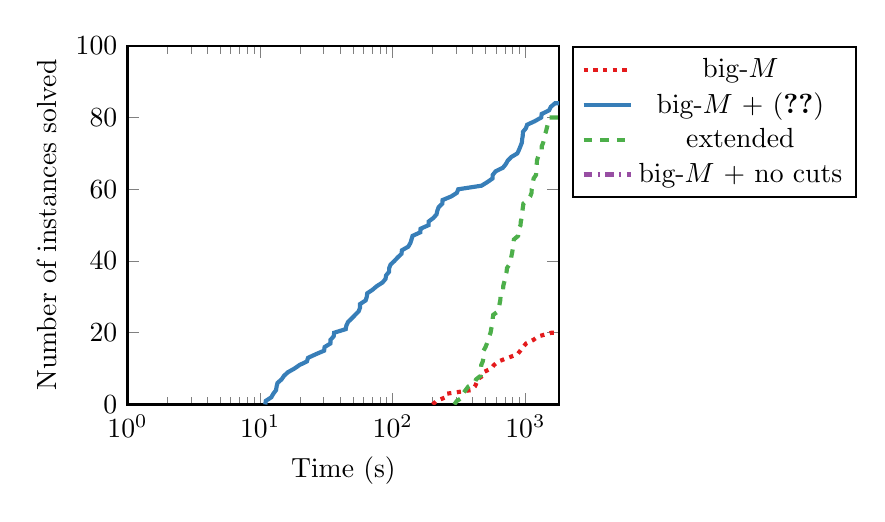
\begin{tikzpicture}
\begin{axis}[
	xlabel=Time (s),
	ylabel=Number of instances solved,
	xmin=1,
	xmax=1800,
	xmode=log,
	ymin=0,
	ymax=100,
	cycle multi list={Set1-4},
	thick,
	legend pos=outer north east,
	x tick label style={/pgf/number format/.cd, set thousands separator={}},
	scale=0.8
    ]

\addplot +[dotted, line width=1.5] coordinates {
(0.000,0)(200.016,0)(213.400,1)(250.701,2)(255.209,3)(389.366,4)(416.042,5)(428.185,6)(434.593,7)(477.248,8)(482.728,9)(549.913,10)(579.752,11)(626.431,12)(737.075,13)(872.758,14)(915.537,15)(958.458,16)(1012.978,17)(1147.197,18)(1256.312,19)(1573.421,20)(1800.000,20)
};

\addplot +[line width=1.5] coordinates { (0,0)
(0.000,0)(10.926,0)(11.029,1)(12.141,2)(12.574,3)(13.178,4)(13.310,5)(13.519,6)(14.511,7)(15.143,8)(16.212,9)(18.118,10)(19.818,11)(22.535,12)(22.964,13)(26.257,14)(30.373,15)(30.620,16)(33.884,17)(33.910,18)(35.863,19)(36.134,20)(44.185,21)(44.710,22)(46.004,23)(49.104,24)(52.136,25)(55.366,26)(56.669,27)(56.678,28)(62.419,29)(63.682,30)(64.232,31)(70.478,32)(75.827,33)(83.694,34)(88.192,35)(89.130,36)(93.818,37)(93.927,38)(96.258,39)(102.785,40)(108.975,41)(116.348,42)(117.292,43)(130.975,44)(135.703,45)(138.493,46)(140.969,47)(161.391,48)(162.063,49)(186.414,50)(186.478,51)(202.393,52)(213.807,53)(216.762,54)(221.753,55)(236.515,56)(237.472,57)(275.902,58)(304.160,59)(311.763,60)(466.913,61)(516.754,62)(564.719,63)(567.466,64)(596.327,65)(676.548,66)(711.947,67)(736.712,68)(783.253,69)(869.017,70)(895.416,71)(917.905,72)(940.710,73)(946.208,74)(955.712,75)(957.823,76)(1008.568,77)(1031.457,78)(1179.609,79)(1315.609,80)(1327.211,81)(1508.650,82)(1556.477,83)(1676.604,84)(1800.000,84)
};

\addplot +[dashed, line width=1.5] coordinates { (0,0)
(0.000,0)(291.123,0)(304.260,1)(337.765,2)(338.746,3)(354.233,4)(370.973,5)(413.280,6)(424.993,7)(460.116,8)(461.748,9)(463.096,10)(464.743,11)(477.083,12)(482.457,13)(483.141,14)(483.467,15)(500.758,16)(512.934,17)(523.865,18)(532.305,19)(546.597,20)(551.939,21)(560.813,22)(566.648,23)(567.355,24)(572.290,25)(625.472,26)(630.244,27)(638.643,28)(646.618,29)(649.133,30)(675.245,31)(678.859,32)(680.776,33)(691.489,34)(704.245,35)(707.126,36)(722.259,37)(725.898,38)(755.967,39)(775.662,40)(781.173,41)(791.785,42)(800.285,43)(808.156,44)(812.561,45)(819.229,46)(881.397,47)(887.791,48)(892.458,49)(918.828,50)(923.877,51)(937.224,52)(941.182,53)(949.978,54)(957.818,55)(965.734,56)(1038.186,57)(1087.226,58)(1113.039,59)(1116.502,60)(1139.682,61)(1139.921,62)(1154.051,63)(1202.194,64)(1211.171,65)(1211.259,66)(1218.455,67)(1222.273,68)(1244.772,69)(1273.453,70)(1327.791,71)(1329.087,72)(1361.641,73)(1384.576,74)(1389.731,75)(1427.386,76)(1448.842,77)(1471.646,78)(1516.231,79)(1517.456,80)(1800.000,80)
};

% Plot for big-$M$ + our cuts + Gurobi cuts. Commented in case we want it later.
% Average time: 1065.71; average gap: 1.55%
% \addplot coordinates {
% (0.000,0)(343.992,0)(351.659,1)(377.114,2)(418.631,3)(460.533,4)(467.214,5)(551.179,6)(553.821,7)(564.796,8)(570.503,9)(576.579,10)(576.611,11)(610.623,12)(616.833,13)(640.949,14)(655.794,15)(685.260,16)(690.705,17)(711.270,18)(729.510,19)(731.061,20)(745.874,21)(748.717,22)(769.924,23)(771.387,24)(792.021,25)(794.934,26)(821.225,27)(837.102,28)(837.562,29)(858.765,30)(862.616,31)(870.306,32)(870.580,33)(901.341,34)(911.134,35)(925.882,36)(959.896,37)(976.299,38)(986.621,39)(1016.646,40)(1043.692,41)(1072.384,42)(1081.009,43)(1134.470,44)(1145.806,45)(1153.021,46)(1219.548,47)(1247.587,48)(1262.812,49)(1280.696,50)(1281.844,51)(1294.661,52)(1323.877,53)(1331.769,54)(1353.637,55)(1369.343,56)(1409.065,57)(1426.437,58)(1440.500,59)(1442.324,60)(1459.729,61)(1473.092,62)(1509.663,63)(1514.715,64)(1543.960,65)(1594.614,66)(1626.371,67)(1647.571,68)(1648.908,69)(1668.510,70)(1740.219,71)(1800.000,71)
% };

\addplot +[dashdotted, line width=1.5] coordinates {
(0.000,0)(1800,0)
};

\legend{big-$M$, big-$M$ + \eqref{eqn:ideal-single-relu-2}, extended, big-$M$ + no cuts}
\end{axis}
\end{tikzpicture}
\end{subfigure}
\par\medskip
\begin{subfigure}{\linewidth}
\subcaption{Network trained with L1 regularization.}
\label{fig:perf-profile-l1}
\centering
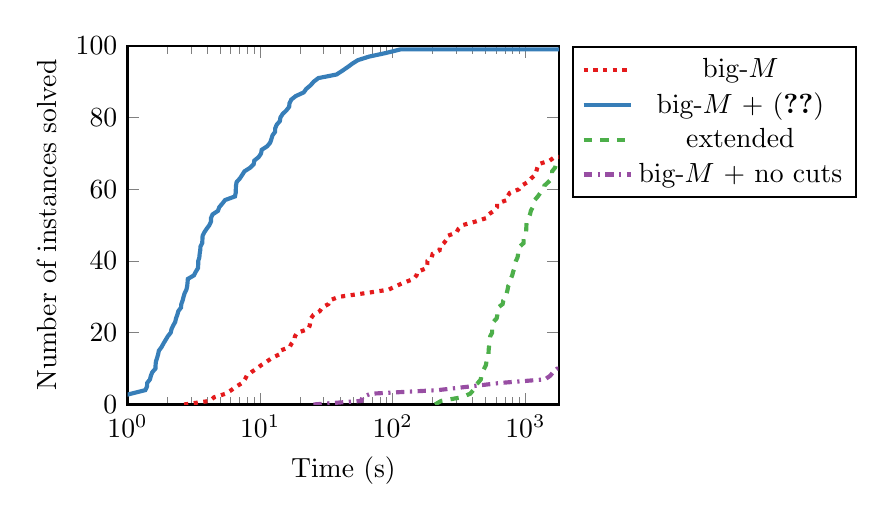
\begin{tikzpicture}
\begin{axis}[
	xlabel=Time (s),
	ylabel=Number of instances solved,
	xmin=1,
	xmax=1800,
	xmode=log,
	ymin=0,
	ymax=100,
	cycle multi list={Set1-4},
	thick,
	legend pos=outer north east,
	x tick label style={/pgf/number format/.cd, set thousands separator={}},
	scale=0.8
    ]

\addplot +[dotted, line width=1.5] coordinates {
(0.000,0)(2.672,0)(4.194,1)(4.495,2)(5.500,3)(6.059,4)(6.617,5)(7.319,6)(7.679,7)(7.933,8)(8.579,9)(9.416,10)(10.214,11)(11.252,12)(12.325,13)(14.003,14)(14.139,15)(16.680,16)(17.267,17)(18.140,18)(18.302,19)(19.062,20)(22.982,21)(23.670,22)(23.851,23)(24.166,24)(25.246,25)(28.146,26)(29.314,27)(32.740,28)(33.392,29)(39.119,30)(61.101,31)(92.941,32)(105.757,33)(121.783,34)(143.929,35)(151.098,36)(153.534,37)(179.871,38)(182.272,39)(182.310,40)(196.572,41)(199.991,42)(225.512,43)(227.084,44)(243.006,45)(255.176,46)(259.267,47)(302.941,48)(313.027,49)(335.576,50)(421.178,51)(510.118,52)(529.271,53)(578.211,54)(611.782,55)(612.747,56)(725.068,57)(732.296,58)(763.151,59)(893.462,60)(934.758,61)(1041.979,62)(1102.970,63)(1184.298,64)(1208.981,65)(1229.530,66)(1254.524,67)(1526.415,68)(1665.686,69)(1800.000,69)
};

\addplot +[line width=1.5] coordinates {
(0.000,0)(0.735,0)(0.801,1)(0.833,2)(1.064,3)(1.363,4)(1.403,5)(1.408,6)(1.477,7)(1.500,8)(1.538,9)(1.624,10)(1.628,11)(1.638,12)(1.672,13)(1.702,14)(1.724,15)(1.807,16)(1.867,17)(1.940,18)(2.012,19)(2.116,20)(2.146,21)(2.209,22)(2.289,23)(2.320,24)(2.376,25)(2.415,26)(2.531,27)(2.545,28)(2.604,29)(2.645,30)(2.695,31)(2.780,32)(2.818,33)(2.836,34)(2.850,35)(3.170,36)(3.271,37)(3.398,38)(3.413,39)(3.414,40)(3.482,41)(3.498,42)(3.537,43)(3.546,44)(3.659,45)(3.671,46)(3.683,47)(3.793,48)(3.956,49)(4.143,50)(4.261,51)(4.262,52)(4.381,53)(4.810,54)(4.917,55)(5.184,56)(5.443,57)(6.458,58)(6.545,59)(6.557,60)(6.576,61)(6.645,62)(7.028,63)(7.326,64)(7.617,65)(8.397,66)(8.939,67)(9.044,68)(9.761,69)(10.163,70)(10.277,71)(11.311,72)(11.905,73)(12.156,74)(12.385,75)(12.953,76)(12.991,77)(13.334,78)(14.081,79)(14.219,80)(14.784,81)(15.786,82)(16.550,83)(16.655,84)(17.168,85)(18.588,86)(21.297,87)(22.294,88)(24.003,89)(25.354,90)(27.488,91)(37.696,92)(41.453,93)(45.450,94)(49.440,95)(54.555,96)(66.422,97)(88.877,98)(114.365,99)(1800.000,99)
};

\addplot +[dashed, line width=1.5] coordinates { (0,0)
(0.000,0)(208.316,0)(231.899,1)(331.030,2)(383.609,3)(405.200,4)(406.205,5)(438.488,6)(461.671,7)(464.766,8)(473.584,9)(489.581,10)(504.198,11)(508.922,12)(509.089,13)(527.268,14)(528.185,15)(531.285,16)(535.875,17)(537.501,18)(542.574,19)(561.391,20)(561.452,21)(568.160,22)(572.659,23)(607.407,24)(614.894,25)(618.583,26)(621.456,27)(674.113,28)(681.671,29)(721.298,30)(722.812,31)(734.094,32)(742.035,33)(772.447,34)(774.719,35)(796.008,36)(808.028,37)(827.122,38)(833.355,39)(848.235,40)(872.496,41)(882.005,42)(885.884,43)(904.149,44)(969.544,45)(969.810,46)(975.263,47)(1011.177,48)(1015.720,49)(1017.963,50)(1024.353,51)(1055.543,52)(1084.240,53)(1099.825,54)(1137.626,55)(1161.919,56)(1175.886,57)(1240.898,58)(1296.375,59)(1376.420,60)(1390.923,61)(1487.599,62)(1582.255,63)(1590.398,64)(1590.811,65)(1671.488,66)(1705.309,67)(1736.513,68)(1800.000,68)
};

\addplot +[dashdotted, line width=1.5] coordinates {
(0.000,0)(25.238,0)(58.059,1)(58.896,2)(68.126,3)(219.182,4)(378.731,5)(646.885,6)(1407.056,7)(1537.978,8)(1617.722,9)(1734.822,10)(1800.000,10)
};

\legend{big-$M$, big-$M$ + \eqref{eqn:ideal-single-relu-2}, extended, big-$M$ + no cuts}
\end{axis}
\end{tikzpicture}
\end{subfigure}
\caption{Number of instances solved within a given amount of time. Curves to the upper left are better, with more instances solved in less time.}
\end{figure}

% \begin{figure}[htbp]
% \begin{center}
% \begin{tikzpicture}
% \begin{axis}[
% 	xlabel=Time (s),
% 	ylabel=Number of instances solved,
% 	xmin=1,
% 	xmax=1800,
% 	xmode=log,
% 	ymin=0,
% 	ymax=100,
% 	cycle multi list={Set1-4},
% 	thick,
% 	legend pos=outer north east,
% 	x tick label style={/pgf/number format/.cd, set thousands separator={}},
% 	scale=0.8
%     ]

% \addplot +[dotted, line width=1.5] coordinates {
% (0.000,0)(200.016,0)(213.400,1)(250.701,2)(255.209,3)(389.366,4)(416.042,5)(428.185,6)(434.593,7)(477.248,8)(482.728,9)(549.913,10)(579.752,11)(626.431,12)(737.075,13)(872.758,14)(915.537,15)(958.458,16)(1012.978,17)(1147.197,18)(1256.312,19)(1573.421,20)(1800.000,20)
% };

% \addplot +[line width=1.5] coordinates { (0,0)
% (0.000,0)(10.926,0)(11.029,1)(12.141,2)(12.574,3)(13.178,4)(13.310,5)(13.519,6)(14.511,7)(15.143,8)(16.212,9)(18.118,10)(19.818,11)(22.535,12)(22.964,13)(26.257,14)(30.373,15)(30.620,16)(33.884,17)(33.910,18)(35.863,19)(36.134,20)(44.185,21)(44.710,22)(46.004,23)(49.104,24)(52.136,25)(55.366,26)(56.669,27)(56.678,28)(62.419,29)(63.682,30)(64.232,31)(70.478,32)(75.827,33)(83.694,34)(88.192,35)(89.130,36)(93.818,37)(93.927,38)(96.258,39)(102.785,40)(108.975,41)(116.348,42)(117.292,43)(130.975,44)(135.703,45)(138.493,46)(140.969,47)(161.391,48)(162.063,49)(186.414,50)(186.478,51)(202.393,52)(213.807,53)(216.762,54)(221.753,55)(236.515,56)(237.472,57)(275.902,58)(304.160,59)(311.763,60)(466.913,61)(516.754,62)(564.719,63)(567.466,64)(596.327,65)(676.548,66)(711.947,67)(736.712,68)(783.253,69)(869.017,70)(895.416,71)(917.905,72)(940.710,73)(946.208,74)(955.712,75)(957.823,76)(1008.568,77)(1031.457,78)(1179.609,79)(1315.609,80)(1327.211,81)(1508.650,82)(1556.477,83)(1676.604,84)(1800.000,84)
% };

% \addplot +[dashed, line width=1.5] coordinates { (0,0)
% (0.000,0)(291.123,0)(304.260,1)(337.765,2)(338.746,3)(354.233,4)(370.973,5)(413.280,6)(424.993,7)(460.116,8)(461.748,9)(463.096,10)(464.743,11)(477.083,12)(482.457,13)(483.141,14)(483.467,15)(500.758,16)(512.934,17)(523.865,18)(532.305,19)(546.597,20)(551.939,21)(560.813,22)(566.648,23)(567.355,24)(572.290,25)(625.472,26)(630.244,27)(638.643,28)(646.618,29)(649.133,30)(675.245,31)(678.859,32)(680.776,33)(691.489,34)(704.245,35)(707.126,36)(722.259,37)(725.898,38)(755.967,39)(775.662,40)(781.173,41)(791.785,42)(800.285,43)(808.156,44)(812.561,45)(819.229,46)(881.397,47)(887.791,48)(892.458,49)(918.828,50)(923.877,51)(937.224,52)(941.182,53)(949.978,54)(957.818,55)(965.734,56)(1038.186,57)(1087.226,58)(1113.039,59)(1116.502,60)(1139.682,61)(1139.921,62)(1154.051,63)(1202.194,64)(1211.171,65)(1211.259,66)(1218.455,67)(1222.273,68)(1244.772,69)(1273.453,70)(1327.791,71)(1329.087,72)(1361.641,73)(1384.576,74)(1389.731,75)(1427.386,76)(1448.842,77)(1471.646,78)(1516.231,79)(1517.456,80)(1800.000,80)
% };

% % Plot for big-$M$ + our cuts + Gurobi cuts. Commented in case we want it later.
% % Average time: 1065.71; average gap: 1.55%
% % \addplot coordinates {
% % (0.000,0)(343.992,0)(351.659,1)(377.114,2)(418.631,3)(460.533,4)(467.214,5)(551.179,6)(553.821,7)(564.796,8)(570.503,9)(576.579,10)(576.611,11)(610.623,12)(616.833,13)(640.949,14)(655.794,15)(685.260,16)(690.705,17)(711.270,18)(729.510,19)(731.061,20)(745.874,21)(748.717,22)(769.924,23)(771.387,24)(792.021,25)(794.934,26)(821.225,27)(837.102,28)(837.562,29)(858.765,30)(862.616,31)(870.306,32)(870.580,33)(901.341,34)(911.134,35)(925.882,36)(959.896,37)(976.299,38)(986.621,39)(1016.646,40)(1043.692,41)(1072.384,42)(1081.009,43)(1134.470,44)(1145.806,45)(1153.021,46)(1219.548,47)(1247.587,48)(1262.812,49)(1280.696,50)(1281.844,51)(1294.661,52)(1323.877,53)(1331.769,54)(1353.637,55)(1369.343,56)(1409.065,57)(1426.437,58)(1440.500,59)(1442.324,60)(1459.729,61)(1473.092,62)(1509.663,63)(1514.715,64)(1543.960,65)(1594.614,66)(1626.371,67)(1647.571,68)(1648.908,69)(1668.510,70)(1740.219,71)(1800.000,71)
% % };

% \addplot +[dashdotted, line width=1.5] coordinates {
% (0.000,0)(1800,0)
% };

% \legend{big-$M$, big-$M$ + \eqref{eqn:ideal-single-relu-2}, extended, big-$M$ + no cuts}
% \end{axis}
% \end{tikzpicture}
% \end{center}
% \caption{Number of instances solved within a given amount of time. Curves to the upper left are better, with more instances solved in less time.}
% \label{fig:perf-profile}
% \end{figure}

\subsection{ReLU network with L1 regularization} \label{ssec:l1-regularization}

The optimization problems studied in Section~\ref{ssec:standard-training} are surprisingly difficult given the relatively small size of the networks involved. This can largely be attributed to the fact that the weights describing the neural network are almost completely dense. To remedy this, we train a second model, using the same network architecture, but with L1 regularization as suggested by Xiao et al.~\cite{Xiao:2018}. We again set a radius of $\epsilon=0.1$, and train for 100 epochs with a learning rate of $5 \cdot 10^{-4}$ and a regularization parameter of $10^{-4}$. \blue{The network achieves a test accuracy of 98.0\%. With regularization, 4\% of the weights in the network are zero, compared to 0.3\% in the previous network. Moreover, with regularization we can infer from variable bounds that on average 73.1\% of the ReLUs are linear within the perturbation box of radius $\epsilon$, enabling us to eliminate the corresponding binary variables. In the first network, we can do so only for 27.8\% of the ReLUs.}

% \blue{The addition of the regularization induces substantial weight sparsity, while incurring only a very modest drop in test accuracy.}

We report the corresponding results in Table~\ref{tab:small-relu-l1} and Figure~\ref{fig:perf-profile-l1}. While the extended approach does not seem to be substantially affected by the network sparsity, the big-$M$-based approaches are able to exploit it to solve more instances, more quickly. The big-$M$ approach is able to solve 70 of 100 instances to optimality within the time limit, though the mean solve time is still quite large. In contrast, the big-$M$ + \eqref{eqn:ideal-single-relu-2} approach fully exploits the sparsity in the model, solving each instance strictly faster than each of the other approaches. Indeed, the approach is able to solve 69 instances in less than 10 seconds, and solves all instances in under 120 seconds.

% \begin{table}[tb]
%     \centering
%     \begin{tabular}{lrrrr}
%         \toprule
%         method & time (s) & optimality gap & win \\ \midrule
%         big-$M$ + \eqref{eqn:ideal-single-relu-2} &  13.65 & 0\% & 100 \\ 
%         big-$M$  & 994.20 & 14.87\% & 0 \\
%         big-$M$ + no cuts & 1730.78 & 80.87\% & 0 \\
%         extended &  1252.86 & 37.45\% & 0 \\
%         \bottomrule\\
%     \end{tabular}
%     \caption{Results for network trained with L1 regularization. Shifted geometric mean for time and optimality gap taken over 100 instances (shift of 10 and 1, respectively). The ``win'' column is the number of (solved) instances on which the method is the fastest.}
%     \label{tab:small-relu-l1}
% \end{table}

% \begin{figure}[htbp]
% \begin{center}
% \begin{tikzpicture}
% \begin{axis}[
% 	xlabel=Time (s),
% 	ylabel=Number of instances solved,
% 	xmin=1,
% 	xmax=1800,
% 	xmode=log,
% 	ymin=0,
% 	ymax=100,
% 	cycle multi list={Set1-4},
% 	thick,
% 	legend pos=outer north east,
% 	x tick label style={/pgf/number format/.cd, set thousands separator={}},
% 	scale=0.8
%     ]

% \addplot +[dotted, line width=1.5] coordinates {
% (0.000,0)(2.672,0)(4.194,1)(4.495,2)(5.500,3)(6.059,4)(6.617,5)(7.319,6)(7.679,7)(7.933,8)(8.579,9)(9.416,10)(10.214,11)(11.252,12)(12.325,13)(14.003,14)(14.139,15)(16.680,16)(17.267,17)(18.140,18)(18.302,19)(19.062,20)(22.982,21)(23.670,22)(23.851,23)(24.166,24)(25.246,25)(28.146,26)(29.314,27)(32.740,28)(33.392,29)(39.119,30)(61.101,31)(92.941,32)(105.757,33)(121.783,34)(143.929,35)(151.098,36)(153.534,37)(179.871,38)(182.272,39)(182.310,40)(196.572,41)(199.991,42)(225.512,43)(227.084,44)(243.006,45)(255.176,46)(259.267,47)(302.941,48)(313.027,49)(335.576,50)(421.178,51)(510.118,52)(529.271,53)(578.211,54)(611.782,55)(612.747,56)(725.068,57)(732.296,58)(763.151,59)(893.462,60)(934.758,61)(1041.979,62)(1102.970,63)(1184.298,64)(1208.981,65)(1229.530,66)(1254.524,67)(1526.415,68)(1665.686,69)(1800.000,69)
% };

% \addplot +[line width=1.5] coordinates {
% (0.000,0)(0.735,0)(0.801,1)(0.833,2)(1.064,3)(1.363,4)(1.403,5)(1.408,6)(1.477,7)(1.500,8)(1.538,9)(1.624,10)(1.628,11)(1.638,12)(1.672,13)(1.702,14)(1.724,15)(1.807,16)(1.867,17)(1.940,18)(2.012,19)(2.116,20)(2.146,21)(2.209,22)(2.289,23)(2.320,24)(2.376,25)(2.415,26)(2.531,27)(2.545,28)(2.604,29)(2.645,30)(2.695,31)(2.780,32)(2.818,33)(2.836,34)(2.850,35)(3.170,36)(3.271,37)(3.398,38)(3.413,39)(3.414,40)(3.482,41)(3.498,42)(3.537,43)(3.546,44)(3.659,45)(3.671,46)(3.683,47)(3.793,48)(3.956,49)(4.143,50)(4.261,51)(4.262,52)(4.381,53)(4.810,54)(4.917,55)(5.184,56)(5.443,57)(6.458,58)(6.545,59)(6.557,60)(6.576,61)(6.645,62)(7.028,63)(7.326,64)(7.617,65)(8.397,66)(8.939,67)(9.044,68)(9.761,69)(10.163,70)(10.277,71)(11.311,72)(11.905,73)(12.156,74)(12.385,75)(12.953,76)(12.991,77)(13.334,78)(14.081,79)(14.219,80)(14.784,81)(15.786,82)(16.550,83)(16.655,84)(17.168,85)(18.588,86)(21.297,87)(22.294,88)(24.003,89)(25.354,90)(27.488,91)(37.696,92)(41.453,93)(45.450,94)(49.440,95)(54.555,96)(66.422,97)(88.877,98)(114.365,99)(1800.000,99)
% };

% \addplot +[dashed, line width=1.5] coordinates { (0,0)
% (0.000,0)(208.316,0)(231.899,1)(331.030,2)(383.609,3)(405.200,4)(406.205,5)(438.488,6)(461.671,7)(464.766,8)(473.584,9)(489.581,10)(504.198,11)(508.922,12)(509.089,13)(527.268,14)(528.185,15)(531.285,16)(535.875,17)(537.501,18)(542.574,19)(561.391,20)(561.452,21)(568.160,22)(572.659,23)(607.407,24)(614.894,25)(618.583,26)(621.456,27)(674.113,28)(681.671,29)(721.298,30)(722.812,31)(734.094,32)(742.035,33)(772.447,34)(774.719,35)(796.008,36)(808.028,37)(827.122,38)(833.355,39)(848.235,40)(872.496,41)(882.005,42)(885.884,43)(904.149,44)(969.544,45)(969.810,46)(975.263,47)(1011.177,48)(1015.720,49)(1017.963,50)(1024.353,51)(1055.543,52)(1084.240,53)(1099.825,54)(1137.626,55)(1161.919,56)(1175.886,57)(1240.898,58)(1296.375,59)(1376.420,60)(1390.923,61)(1487.599,62)(1582.255,63)(1590.398,64)(1590.811,65)(1671.488,66)(1705.309,67)(1736.513,68)(1800.000,68)
% };

% \addplot +[dashdotted, line width=1.5] coordinates {
% (0.000,0)(25.238,0)(58.059,1)(58.896,2)(68.126,3)(219.182,4)(378.731,5)(646.885,6)(1407.056,7)(1537.978,8)(1617.722,9)(1734.822,10)(1800.000,10)
% };

% \legend{big-$M$, big-$M$ + \eqref{eqn:ideal-single-relu-2}, extended, big-$M$ + no cuts}
% \end{axis}
% \end{tikzpicture}
% \end{center}
% \caption{Number of L1-regularized instances solved within a given amount of time. Curves to the upper left are better, with more instances solved in less time.}
% \label{fig:perf-profile-l1}
% \end{figure}


% We emulate the computational setting used by Xiao et al.~\cite{Xiao:2018}, using the same network configuration and sizes: two convolutional layers feeding into a dense layer, each with ReLU nonlinearities. Moreover, we use the same training procedure, incorporating adversarial training using the fast gradient sign method, L1 regularization, and a ``ReLU stability'' loss term. Finally, we augment the solver with a primal feasible solution produced by a local search heuristic. \jpnote{I think the reason for the heursitic should be expanded. Does Xiao et all use it?}

% We use network architecture summarized in Figure~\ref{fig:tf-pseudocode}, with two convolutional layers (with ReLU nonlinearities) and a subsequent dense layers, also with ReLU nonlinearities. We train the network using the Adam algorithm~\cite{Kingma:2014}, running for 70 epochs with a learning rate of $10^{-4}$, attaining a test accuracy of $98.77\%$. We generate 100 adversarial instances by randomly selecting a test image $\tilde{x}$ with actual label $i$, along with a random target adversarial class $j \neq i$. We select a perturbation ball radius of $\epsilon = 0.1$. Note that our evaluation is slightly different than that of Xiao et al~\cite{Xiao:2018}, as we attempt to solve each instance to optimality, rather than terminating immediately after proving a bound less than zero.

% We use the Gurobi v7.5.2 solver, running with a single thread on a machine with 128 GB of RAM and 32 CPUs at 2.30 GHz. We perform our experiments using the \texttt{tf.opt} package for optimization over trained neural networks; \texttt{tf.opt} is under active development at Google, with the intention to open source the project in the future. We  set a time limit of 30 minutes (1800 s) for each run.

% We consider four algorithmic approaches applied to each ReLU neuron in the network:
% \begin{enumerate}
%     \item \underline{big-$M$}: The standard big-$M$ formulation \eqref{eqn:relu-big-M}.
%     \item \underline{big-$M$ + cuts}: The big-$M$ formulation \eqref{eqn:relu-big-M}, along with separation of \eqref{eqn:ideal-single-relu-2}.
%     \item \underline{big-$M$ + root cuts}: The big-$M$ formulation \eqref{eqn:relu-big-M}, along with separation of \eqref{eqn:ideal-single-relu-2} only at the root node.
%     \item \underline{extended}: The extended formulation \eqref{eqn:relu-ideal-extended}.
% \end{enumerate}

% \pgfplotsset{cycle list/Set1-4}
% \begin{figure}[htpb]
% \begin{tikzpicture}
% \begin{axis}[
% 	xlabel=Time (s),
% 	ylabel=Number of instances solved,
% 	xmin=1,
% 	xmax=1800,
% 	xmode=log,
% 	ymin=0,
% 	ymax=100,
% 	cycle multi list={Set1-4},
% 	thick,
% 	legend pos=outer north east,
% 	log ticks with fixed point,
% 	x tick label style={/pgf/number format/.cd, set thousands separator={}},
% 	scale=0.8
%     ]

% \addplot +[line width=1.5] coordinates {
% (0.000,0)(7.571,0)(7.767,1)(9.783,2)(10.016,3)(10.148,4)(10.725,5)(11.145,6)(11.462,7)(11.891,8)(13.172,9)(13.247,10)(13.721,11)(14.308,12)(14.506,13)(14.606,14)(16.898,15)(19.001,16)(21.152,17)(21.729,18)(21.855,19)(22.512,20)(22.761,21)(22.811,22)(26.952,23)(27.458,24)(29.661,25)(31.303,26)(33.862,27)(34.936,28)(37.558,29)(37.999,30)(38.155,31)(40.819,32)(44.917,33)(45.718,34)(47.686,35)(48.703,36)(49.721,37)(51.432,38)(55.173,39)(56.493,40)(57.716,41)(57.822,42)(59.603,43)(62.108,44)(66.664,45)(71.021,46)(72.551,47)(74.771,48)(77.706,49)(83.434,50)(86.263,51)(88.785,52)(92.881,53)(94.236,54)(98.250,55)(99.385,56)(109.352,57)(110.164,58)(110.686,59)(112.739,60)(122.203,61)(125.623,62)(128.229,63)(128.342,64)(147.076,65)(164.393,66)(197.309,67)(218.463,68)(242.242,69)(273.243,70)(290.601,71)(315.407,72)(325.729,73)(338.798,74)(341.712,75)(345.094,76)(532.698,77)(743.000,78)(761.199,79)(1017.610,80)(1800.000,80)
% };

% \addplot +[line width=1.5] coordinates {
% (0.000,0)(5.377,0)(7.126,1)(7.203,2)(7.479,3)(7.516,4)(8.446,5)(8.454,6)(8.509,7)(8.749,8)(9.432,9)(11.975,10)(12.408,11)(12.720,12)(12.922,13)(13.016,14)(13.710,15)(13.790,16)(15.238,17)(15.932,18)(17.036,19)(18.008,20)(18.183,21)(18.963,22)(20.642,23)(20.683,24)(21.140,25)(21.854,26)(22.281,27)(25.357,28)(26.377,29)(29.452,30)(30.291,31)(31.109,32)(31.119,33)(31.164,34)(31.393,35)(32.457,36)(33.956,37)(35.010,38)(36.502,39)(39.723,40)(40.125,41)(42.191,42)(42.646,43)(42.912,44)(43.523,45)(44.378,46)(45.297,47)(47.169,48)(47.718,49)(48.684,50)(49.167,51)(52.917,52)(54.482,53)(62.240,54)(65.383,55)(68.886,56)(72.747,57)(74.390,58)(79.993,59)(85.828,60)(85.864,61)(88.639,62)(103.444,63)(108.593,64)(116.644,65)(120.117,66)(123.343,67)(127.479,68)(134.949,69)(155.143,70)(160.210,71)(198.861,72)(334.942,73)(357.473,74)(364.787,75)(366.970,76)(479.971,77)(567.100,78)(581.201,79)(870.952,80)(1608.960,81)(1800.000,81)
% };

% \addplot +[line width=1.5] coordinates {
% (0.000,0)(6.214,0)(6.644,1)(6.754,2)(7.306,3)(7.318,4)(7.509,5)(7.661,6)(8.699,7)(8.922,8)(9.623,9)(12.381,10)(12.660,11)(13.063,12)(13.201,13)(13.531,14)(13.917,15)(14.034,16)(15.243,17)(17.108,18)(17.192,19)(17.850,20)(18.401,21)(18.859,22)(18.865,23)(19.036,24)(19.322,25)(20.498,26)(26.127,27)(26.872,28)(28.285,29)(29.285,30)(29.742,31)(30.356,32)(32.641,33)(33.554,34)(33.807,35)(34.091,36)(36.740,37)(37.120,38)(37.454,39)(37.504,40)(37.803,41)(40.887,42)(41.471,43)(42.543,44)(43.693,45)(44.931,46)(45.740,47)(47.210,48)(48.435,49)(49.247,50)(52.803,51)(54.296,52)(54.429,53)(55.455,54)(58.864,55)(64.583,56)(69.824,57)(75.637,58)(81.504,59)(87.450,60)(97.732,61)(99.274,62)(106.209,63)(106.442,64)(111.303,65)(124.413,66)(125.157,67)(158.432,68)(217.622,69)(220.577,70)(224.385,71)(318.570,72)(565.408,73)(693.018,74)(796.156,75)(803.173,76)(828.940,77)(894.473,78)(907.943,79)(1383.183,80)(1569.313,81)(1784.367,82)(1800.000,82)
% };

% \addplot +[line width=1.5] coordinates {
% (0.000,0)(261.777,0)(261.816,1)(284.548,2)(311.034,3)(513.084,4)(608.305,5)(852.230,6)(894.070,7)(967.296,8)(1071.282,9)(1080.660,10)(1088.038,11)(1135.920,12)(1142.805,13)(1158.012,14)(1218.106,15)(1325.028,16)(1355.790,17)(1400.452,18)(1403.622,19)(1434.338,20)(1481.998,21)(1514.335,22)(1593.568,23)(1608.699,24)(1753.872,25)(1800.000,25)
% };

% \legend{big-$M$, big-$M$ + cuts, big-$M$ + root cuts, extended}
% \end{axis}
% \end{tikzpicture}
% \caption{Number of instances (out of 100) solved to optimality within a given time frame. Note the logarithmic scale on time.}
% \label{fig:completion-plot}
% \end{figure}

% \begin{figure}[htpb]

% \begin{tikzpicture}
% \begin{axis}[
%       xlabel=$\tau$,
%       ylabel=Instances with performance ratio $\leq \tau$,
%       xmin=1,
%       xmax=16,
%       xmode=log,
%       ymin=0,
%       ymax=1,
%       cycle multi list={Set1-4},
%       thick,
%       legend pos=outer north east,
%       log ticks with fixed point,
%       xtick={1,2,4,8,16},
%       % max space between ticks = 16,
%       xminorticks=true,
%       % x tick label style={/pgf/number format/.cd,1000 sep={\,}},
%       scale=0.8
%   ]

% \addplot +[line width=1] coordinates {
% (1.000,0.078)(1.003,0.078)(1.006,0.078)(1.008,0.078)(1.011,0.078)(1.014,0.078)(1.017,0.078)(1.020,0.078)(1.022,0.078)(1.025,0.089)(1.028,0.089)(1.031,0.100)(1.034,0.100)(1.037,0.111)(1.040,0.111)(1.043,0.111)(1.045,0.111)(1.048,0.111)(1.051,0.111)(1.054,0.111)(1.057,0.111)(1.060,0.111)(1.063,0.122)(1.066,0.133)(1.069,0.133)(1.072,0.133)(1.075,0.156)(1.078,0.156)(1.081,0.156)(1.084,0.156)(1.087,0.167)(1.090,0.167)(1.093,0.167)(1.096,0.167)(1.099,0.167)(1.102,0.167)(1.105,0.167)(1.108,0.167)(1.111,0.178)(1.114,0.178)(1.117,0.178)(1.121,0.178)(1.124,0.178)(1.127,0.178)(1.130,0.178)(1.133,0.189)(1.136,0.189)(1.139,0.189)(1.142,0.189)(1.146,0.189)(1.149,0.200)(1.152,0.200)(1.155,0.211)(1.158,0.211)(1.162,0.211)(1.165,0.211)(1.168,0.211)(1.171,0.222)(1.175,0.222)(1.178,0.222)(1.181,0.233)(1.184,0.233)(1.188,0.244)(1.191,0.244)(1.194,0.244)(1.198,0.256)(1.201,0.256)(1.204,0.256)(1.208,0.267)(1.211,0.278)(1.214,0.289)(1.218,0.289)(1.221,0.311)(1.225,0.311)(1.228,0.311)(1.231,0.311)(1.235,0.311)(1.238,0.311)(1.242,0.322)(1.245,0.322)(1.249,0.322)(1.252,0.333)(1.256,0.333)(1.259,0.333)(1.263,0.344)(1.266,0.344)(1.270,0.344)(1.273,0.344)(1.277,0.344)(1.280,0.344)(1.284,0.344)(1.287,0.344)(1.291,0.344)(1.294,0.344)(1.298,0.344)(1.302,0.344)(1.305,0.356)(1.309,0.356)(1.313,0.356)(1.316,0.356)(1.320,0.356)(1.324,0.356)(1.327,0.356)(1.331,0.356)(1.335,0.367)(1.338,0.367)(1.342,0.367)(1.346,0.367)(1.350,0.367)(1.353,0.367)(1.357,0.367)(1.361,0.378)(1.365,0.378)(1.368,0.378)(1.372,0.378)(1.376,0.378)(1.380,0.378)(1.384,0.378)(1.387,0.389)(1.391,0.400)(1.395,0.411)(1.399,0.411)(1.403,0.411)(1.407,0.422)(1.411,0.422)(1.415,0.422)(1.419,0.433)(1.423,0.433)(1.427,0.433)(1.430,0.433)(1.434,0.444)(1.438,0.444)(1.442,0.444)(1.446,0.456)(1.450,0.456)(1.455,0.467)(1.459,0.467)(1.463,0.467)(1.467,0.478)(1.471,0.489)(1.475,0.500)(1.479,0.500)(1.483,0.511)(1.487,0.511)(1.491,0.511)(1.495,0.511)(1.500,0.511)(1.504,0.511)(1.508,0.511)(1.512,0.522)(1.516,0.522)(1.521,0.533)(1.525,0.544)(1.529,0.544)(1.533,0.544)(1.538,0.556)(1.542,0.556)(1.546,0.556)(1.550,0.556)(1.555,0.556)(1.559,0.556)(1.563,0.556)(1.568,0.556)(1.572,0.556)(1.576,0.556)(1.581,0.556)(1.585,0.556)(1.590,0.556)(1.594,0.567)(1.598,0.567)(1.603,0.567)(1.607,0.567)(1.612,0.578)(1.616,0.578)(1.621,0.578)(1.625,0.578)(1.630,0.578)(1.634,0.578)(1.639,0.578)(1.643,0.578)(1.648,0.578)(1.653,0.578)(1.657,0.578)(1.662,0.578)(1.666,0.589)(1.671,0.589)(1.676,0.589)(1.680,0.589)(1.685,0.589)(1.690,0.589)(1.694,0.589)(1.699,0.589)(1.704,0.589)(1.709,0.589)(1.713,0.589)(1.718,0.589)(1.723,0.600)(1.728,0.611)(1.732,0.622)(1.737,0.622)(1.742,0.622)(1.747,0.622)(1.752,0.622)(1.757,0.622)(1.762,0.622)(1.766,0.622)(1.771,0.622)(1.776,0.622)(1.781,0.622)(1.786,0.622)(1.791,0.622)(1.796,0.622)(1.801,0.633)(1.806,0.633)(1.811,0.633)(1.816,0.633)(1.821,0.633)(1.826,0.633)(1.831,0.633)(1.836,0.644)(1.841,0.644)(1.847,0.644)(1.852,0.644)(1.857,0.644)(1.862,0.644)(1.867,0.644)(1.872,0.644)(1.878,0.644)(1.883,0.644)(1.888,0.644)(1.893,0.644)(1.899,0.644)(1.904,0.644)(1.909,0.644)(1.914,0.644)(1.920,0.644)(1.925,0.644)(1.930,0.644)(1.936,0.644)(1.941,0.644)(1.947,0.644)(1.952,0.644)(1.957,0.667)(1.963,0.667)(1.968,0.667)(1.974,0.678)(1.979,0.678)(1.985,0.678)(1.990,0.689)(1.996,0.689)(2.001,0.700)(2.007,0.700)(2.013,0.700)(2.018,0.700)(2.024,0.700)(2.029,0.700)(2.035,0.700)(2.041,0.711)(2.046,0.711)(2.052,0.711)(2.058,0.711)(2.063,0.711)(2.069,0.711)(2.075,0.711)(2.081,0.711)(2.086,0.711)(2.092,0.711)(2.098,0.711)(2.104,0.711)(2.110,0.711)(2.116,0.711)(2.122,0.711)(2.127,0.711)(2.133,0.711)(2.139,0.711)(2.145,0.711)(2.151,0.711)(2.157,0.711)(2.163,0.711)(2.169,0.711)(2.175,0.711)(2.181,0.711)(2.187,0.722)(2.193,0.733)(2.199,0.733)(2.206,0.733)(2.212,0.733)(2.218,0.733)(2.224,0.733)(2.230,0.744)(2.236,0.744)(2.243,0.744)(2.249,0.744)(2.255,0.744)(2.261,0.744)(2.268,0.744)(2.274,0.744)(2.280,0.744)(2.287,0.744)(2.293,0.744)(2.299,0.744)(2.306,0.744)(2.312,0.744)(2.319,0.744)(2.325,0.744)(2.331,0.744)(2.338,0.744)(2.344,0.744)(2.351,0.744)(2.357,0.744)(2.364,0.744)(2.371,0.744)(2.377,0.744)(2.384,0.744)(2.390,0.744)(2.397,0.744)(2.404,0.744)(2.410,0.744)(2.417,0.744)(2.424,0.744)(2.431,0.744)(2.437,0.756)(2.444,0.756)(2.451,0.756)(2.458,0.756)(2.465,0.756)(2.471,0.756)(2.478,0.756)(2.485,0.756)(2.492,0.756)(2.499,0.756)(2.506,0.756)(2.513,0.756)(2.520,0.756)(2.527,0.756)(2.534,0.756)(2.541,0.756)(2.548,0.756)(2.555,0.756)(2.562,0.756)(2.569,0.756)(2.576,0.756)(2.584,0.756)(2.591,0.756)(2.598,0.756)(2.605,0.756)(2.612,0.756)(2.620,0.756)(2.627,0.756)(2.634,0.756)(2.642,0.756)(2.649,0.756)(2.656,0.756)(2.664,0.756)(2.671,0.756)(2.678,0.756)(2.686,0.756)(2.693,0.756)(2.701,0.756)(2.708,0.756)(2.716,0.756)(2.723,0.756)(2.731,0.756)(2.739,0.756)(2.746,0.756)(2.754,0.756)(2.762,0.756)(2.769,0.756)(2.777,0.756)(2.785,0.756)(2.792,0.756)(2.800,0.756)(2.808,0.756)(2.816,0.756)(2.824,0.756)(2.831,0.756)(2.839,0.756)(2.847,0.756)(2.855,0.756)(2.863,0.756)(2.871,0.756)(2.879,0.756)(2.887,0.756)(2.895,0.756)(2.903,0.756)(2.911,0.756)(2.919,0.756)(2.927,0.756)(2.935,0.756)(2.944,0.756)(2.952,0.756)(2.960,0.756)(2.968,0.756)(2.976,0.756)(2.985,0.756)(2.993,0.756)(3.001,0.756)(3.010,0.756)(3.018,0.756)(3.026,0.756)(3.035,0.756)(3.043,0.756)(3.052,0.756)(3.060,0.756)(3.069,0.756)(3.077,0.756)(3.086,0.756)(3.094,0.756)(3.103,0.756)(3.112,0.756)(3.120,0.756)(3.129,0.756)(3.138,0.756)(3.146,0.756)(3.155,0.756)(3.164,0.756)(3.173,0.756)(3.181,0.756)(3.190,0.756)(3.199,0.756)(3.208,0.756)(3.217,0.756)(3.226,0.756)(3.235,0.756)(3.244,0.756)(3.253,0.756)(3.262,0.756)(3.271,0.756)(3.280,0.756)(3.289,0.756)(3.298,0.756)(3.307,0.756)(3.317,0.756)(3.326,0.756)(3.335,0.756)(3.344,0.756)(3.354,0.756)(3.363,0.756)(3.372,0.756)(3.382,0.756)(3.391,0.756)(3.401,0.756)(3.410,0.756)(3.419,0.756)(3.429,0.756)(3.439,0.756)(3.448,0.767)(3.458,0.767)(3.467,0.767)(3.477,0.767)(3.487,0.767)(3.496,0.767)(3.506,0.767)(3.516,0.767)(3.525,0.767)(3.535,0.767)(3.545,0.767)(3.555,0.767)(3.565,0.767)(3.575,0.767)(3.585,0.767)(3.595,0.767)(3.605,0.767)(3.615,0.767)(3.625,0.767)(3.635,0.767)(3.645,0.767)(3.655,0.767)(3.665,0.778)(3.675,0.778)(3.686,0.778)(3.696,0.778)(3.706,0.778)(3.716,0.778)(3.727,0.778)(3.737,0.778)(3.747,0.778)(3.758,0.778)(3.768,0.778)(3.779,0.778)(3.789,0.778)(3.800,0.778)(3.810,0.778)(3.821,0.778)(3.832,0.778)(3.842,0.778)(3.853,0.778)(3.864,0.778)(3.874,0.778)(3.885,0.778)(3.896,0.778)(3.907,0.778)(3.918,0.778)(3.928,0.778)(3.939,0.778)(3.950,0.778)(3.961,0.778)(3.972,0.778)(3.983,0.778)(3.994,0.778)(4.006,0.778)(4.017,0.778)(4.028,0.778)(4.039,0.778)(4.050,0.778)(4.062,0.778)(4.073,0.778)(4.084,0.778)(4.095,0.778)(4.107,0.778)(4.118,0.778)(4.130,0.778)(4.141,0.778)(4.153,0.778)(4.164,0.778)(4.176,0.778)(4.187,0.778)(4.199,0.778)(4.211,0.778)(4.222,0.778)(4.234,0.789)(4.246,0.789)(4.258,0.789)(4.270,0.789)(4.281,0.800)(4.293,0.800)(4.305,0.800)(4.317,0.800)(4.329,0.800)(4.341,0.800)(4.353,0.800)(4.365,0.800)(4.378,0.800)(4.390,0.800)(4.402,0.800)(4.414,0.800)(4.426,0.800)(4.439,0.800)(4.451,0.800)(4.463,0.800)(4.476,0.800)(4.488,0.800)(4.501,0.800)(4.513,0.800)(4.526,0.800)(4.538,0.800)(4.551,0.800)(4.564,0.800)(4.576,0.800)(4.589,0.800)(4.602,0.800)(4.615,0.800)(4.627,0.800)(4.640,0.800)(4.653,0.800)(4.666,0.800)(4.679,0.800)(4.692,0.800)(4.705,0.800)(4.718,0.800)(4.731,0.800)(4.744,0.800)(4.758,0.800)(4.771,0.800)(4.784,0.800)(4.797,0.800)(4.811,0.800)(4.824,0.800)(4.838,0.800)(4.851,0.800)(4.864,0.800)(4.878,0.800)(4.892,0.800)(4.905,0.800)(4.919,0.800)(4.932,0.800)(4.946,0.800)(4.960,0.811)(4.974,0.811)(4.988,0.811)(5.001,0.811)(5.015,0.811)(5.029,0.811)(5.043,0.811)(5.057,0.811)(5.071,0.811)(5.085,0.811)(5.099,0.811)(5.114,0.811)(5.128,0.811)(5.142,0.811)(5.156,0.811)(5.171,0.811)(5.185,0.811)(5.200,0.811)(5.214,0.811)(5.228,0.811)(5.243,0.811)(5.258,0.811)(5.272,0.811)(5.287,0.811)(5.302,0.811)(5.316,0.811)(5.331,0.811)(5.346,0.811)(5.361,0.811)(5.376,0.811)(5.391,0.822)(5.406,0.822)(5.421,0.822)(5.436,0.822)(5.451,0.822)(5.466,0.822)(5.481,0.822)(5.496,0.822)(5.512,0.822)(5.527,0.822)(5.542,0.822)(5.558,0.822)(5.573,0.822)(5.589,0.822)(5.604,0.822)(5.620,0.822)(5.635,0.822)(5.651,0.822)(5.667,0.822)(5.682,0.822)(5.698,0.822)(5.714,0.822)(5.730,0.822)(5.746,0.822)(5.762,0.822)(5.778,0.822)(5.794,0.822)(5.810,0.822)(5.826,0.822)(5.842,0.822)(5.859,0.822)(5.875,0.822)(5.891,0.822)(5.908,0.822)(5.924,0.822)(5.940,0.822)(5.957,0.822)(5.974,0.822)(5.990,0.822)(6.007,0.822)(6.023,0.822)(6.040,0.822)(6.057,0.822)(6.074,0.822)(6.091,0.822)(6.108,0.822)(6.125,0.822)(6.142,0.822)(6.159,0.822)(6.176,0.822)(6.193,0.833)(6.210,0.833)(6.227,0.833)(6.245,0.833)(6.262,0.833)(6.280,0.833)(6.297,0.833)(6.314,0.833)(6.332,0.833)(6.350,0.833)(6.367,0.833)(6.385,0.833)(6.403,0.833)(6.420,0.833)(6.438,0.833)(6.456,0.833)(6.474,0.833)(6.492,0.833)(6.510,0.833)(6.528,0.833)(6.546,0.833)(6.565,0.833)(6.583,0.833)(6.601,0.833)(6.620,0.833)(6.638,0.833)(6.656,0.833)(6.675,0.833)(6.693,0.833)(6.712,0.833)(6.731,0.833)(6.749,0.833)(6.768,0.833)(6.787,0.833)(6.806,0.833)(6.825,0.833)(6.844,0.833)(6.863,0.833)(6.882,0.833)(6.901,0.833)(6.920,0.833)(6.939,0.833)(6.959,0.833)(6.978,0.833)(6.997,0.844)(7.017,0.844)(7.036,0.844)(7.056,0.844)(7.075,0.844)(7.095,0.844)(7.115,0.844)(7.135,0.844)(7.154,0.844)(7.174,0.844)(7.194,0.844)(7.214,0.844)(7.234,0.844)(7.254,0.844)(7.275,0.844)(7.295,0.844)(7.315,0.844)(7.335,0.844)(7.356,0.844)(7.376,0.844)(7.397,0.844)(7.417,0.844)(7.438,0.844)(7.459,0.844)(7.479,0.844)(7.500,0.844)(7.521,0.844)(7.542,0.844)(7.563,0.844)(7.584,0.844)(7.605,0.844)(7.626,0.844)(7.647,0.844)(7.668,0.844)(7.690,0.844)(7.711,0.844)(7.733,0.844)(7.754,0.844)(7.776,0.844)(7.797,0.844)(7.819,0.844)(7.841,0.844)(7.862,0.844)(7.884,0.844)(7.906,0.844)(7.928,0.844)(7.950,0.844)(7.972,0.844)(7.994,0.844)(8.017,0.844)(8.039,0.844)(8.061,0.844)(8.084,0.844)(8.106,0.844)(8.129,0.856)(8.151,0.856)(8.174,0.856)(8.197,0.867)(8.219,0.867)(8.242,0.867)(8.265,0.867)(8.288,0.867)(8.311,0.867)(8.334,0.867)(8.357,0.867)(8.381,0.867)(8.404,0.867)(8.427,0.867)(8.451,0.867)(8.474,0.867)(8.498,0.867)(8.521,0.867)(8.545,0.867)(8.569,0.867)(8.593,0.867)(8.617,0.867)(8.640,0.867)(8.664,0.867)(8.689,0.867)(8.713,0.867)(8.737,0.867)(8.761,0.867)(8.786,0.867)(8.810,0.867)(8.834,0.867)(8.859,0.867)(8.884,0.867)(8.908,0.867)(8.933,0.867)(8.958,0.867)(8.983,0.867)(9.008,0.867)(9.033,0.867)(9.058,0.867)(9.083,0.867)(9.108,0.867)(9.134,0.867)(9.159,0.867)(9.184,0.867)(9.210,0.867)(9.236,0.867)(9.261,0.867)(9.287,0.867)(9.313,0.867)(9.339,0.867)(9.365,0.867)(9.391,0.867)(9.417,0.867)(9.443,0.867)(9.469,0.867)(9.496,0.867)(9.522,0.867)(9.548,0.867)(9.575,0.867)(9.602,0.867)(9.628,0.867)(9.655,0.867)(9.682,0.867)(9.709,0.867)(9.736,0.867)(9.763,0.867)(9.790,0.867)(9.817,0.867)(9.844,0.867)(9.872,0.867)(9.899,0.867)(9.927,0.867)(9.954,0.878)(9.982,0.878)(10.010,0.878)(10.037,0.878)(10.065,0.878)(10.093,0.878)(10.121,0.878)(10.150,0.878)(10.178,0.878)(10.206,0.878)(10.234,0.878)(10.263,0.878)(10.291,0.878)(10.320,0.878)(10.349,0.878)(10.377,0.878)(10.406,0.878)(10.435,0.878)(10.464,0.878)(10.493,0.878)(10.522,0.878)(10.552,0.878)(10.581,0.878)(10.610,0.878)(10.640,0.878)(10.669,0.878)(10.699,0.878)(10.729,0.878)(10.759,0.878)(10.789,0.878)(10.819,0.878)(10.849,0.878)(10.879,0.878)(10.909,0.878)(10.939,0.878)(10.970,0.878)(11.000,0.878)(11.031,0.878)(11.061,0.878)(11.092,0.878)(11.123,0.878)(11.154,0.878)(11.185,0.878)(11.216,0.878)(11.247,0.878)(11.278,0.878)(11.310,0.878)(11.341,0.878)(11.373,0.878)(11.404,0.878)(11.436,0.878)(11.468,0.878)(11.500,0.878)(11.532,0.878)(11.564,0.878)(11.596,0.878)(11.628,0.878)(11.660,0.878)(11.693,0.878)(11.725,0.878)(11.758,0.878)(11.791,0.878)(11.823,0.878)(11.856,0.878)(11.889,0.878)(11.922,0.878)(11.955,0.878)(11.989,0.878)(12.022,0.878)(12.055,0.878)(12.089,0.878)(12.122,0.878)(12.156,0.878)(12.190,0.878)(12.224,0.889)(12.258,0.889)(12.292,0.889)(12.326,0.889)(12.360,0.889)(12.395,0.889)(12.429,0.889)(12.464,0.889)(12.498,0.889)(12.533,0.889)(12.568,0.889)(12.603,0.889)(12.638,0.889)(12.673,0.889)(12.708,0.889)(12.743,0.889)(12.779,0.889)(12.814,0.889)(12.850,0.889)(12.886,0.889)(12.921,0.889)(12.957,0.889)(12.993,0.889)(13.029,0.889)(13.066,0.889)(13.102,0.889)(13.138,0.889)(13.175,0.889)(13.212,0.889)(13.248,0.889)(13.285,0.889)(13.322,0.889)(13.359,0.889)(13.396,0.889)(13.433,0.889)(13.471,0.889)(13.508,0.889)(13.546,0.889)(13.583,0.889)(13.621,0.889)(13.659,0.889)(13.697,0.889)(13.735,0.889)(13.773,0.889)(13.811,0.889)(13.850,0.889)(13.888,0.889)(13.927,0.889)(13.966,0.889)(14.004,0.889)(14.043,0.889)(14.082,0.889)(14.121,0.889)(14.161,0.889)(14.200,0.889)(14.240,0.889)(14.279,0.889)(14.319,0.889)(14.359,0.889)(14.399,0.889)(14.439,0.889)(14.479,0.889)(14.519,0.889)(14.559,0.889)(14.600,0.889)(14.640,0.889)(14.681,0.889)(14.722,0.889)(14.763,0.889)(14.804,0.889)(14.845,0.889)(14.886,0.889)(14.927,0.889)(14.969,0.889)(15.011,0.889)(15.052,0.889)(15.094,0.889)(15.136,0.889)(15.178,0.889)(15.220,0.889)(15.263,0.889)(15.305,0.889)(15.348,0.889)(15.390,0.889)(15.433,0.889)(15.476,0.889)(15.519,0.889)(15.562,0.889)(15.605,0.889)(15.649,0.889)(15.692,0.889)(15.736,0.889)(15.780,0.889)(15.823,0.889)(15.867,0.889)(15.911,0.889)(15.956,0.889)(16.000,0.889)
% };

% \addplot +[line width=1] coordinates {
% (1.000,0.500)(1.003,0.500)(1.006,0.511)(1.008,0.511)(1.011,0.511)(1.014,0.511)(1.017,0.522)(1.020,0.533)(1.022,0.533)(1.025,0.533)(1.028,0.567)(1.031,0.567)(1.034,0.578)(1.037,0.589)(1.040,0.600)(1.043,0.600)(1.045,0.600)(1.048,0.600)(1.051,0.600)(1.054,0.600)(1.057,0.611)(1.060,0.633)(1.063,0.656)(1.066,0.656)(1.069,0.656)(1.072,0.667)(1.075,0.667)(1.078,0.667)(1.081,0.667)(1.084,0.667)(1.087,0.667)(1.090,0.667)(1.093,0.667)(1.096,0.667)(1.099,0.667)(1.102,0.667)(1.105,0.667)(1.108,0.667)(1.111,0.667)(1.114,0.678)(1.117,0.678)(1.121,0.678)(1.124,0.678)(1.127,0.678)(1.130,0.689)(1.133,0.689)(1.136,0.689)(1.139,0.689)(1.142,0.700)(1.146,0.700)(1.149,0.700)(1.152,0.711)(1.155,0.711)(1.158,0.711)(1.162,0.711)(1.165,0.722)(1.168,0.722)(1.171,0.722)(1.175,0.722)(1.178,0.722)(1.181,0.722)(1.184,0.722)(1.188,0.722)(1.191,0.722)(1.194,0.722)(1.198,0.722)(1.201,0.733)(1.204,0.733)(1.208,0.733)(1.211,0.733)(1.214,0.733)(1.218,0.733)(1.221,0.733)(1.225,0.733)(1.228,0.733)(1.231,0.733)(1.235,0.733)(1.238,0.733)(1.242,0.733)(1.245,0.733)(1.249,0.733)(1.252,0.733)(1.256,0.733)(1.259,0.733)(1.263,0.733)(1.266,0.733)(1.270,0.733)(1.273,0.733)(1.277,0.733)(1.280,0.733)(1.284,0.733)(1.287,0.733)(1.291,0.733)(1.294,0.733)(1.298,0.733)(1.302,0.733)(1.305,0.733)(1.309,0.744)(1.313,0.744)(1.316,0.744)(1.320,0.744)(1.324,0.744)(1.327,0.744)(1.331,0.744)(1.335,0.744)(1.338,0.744)(1.342,0.744)(1.346,0.744)(1.350,0.744)(1.353,0.744)(1.357,0.744)(1.361,0.744)(1.365,0.744)(1.368,0.744)(1.372,0.744)(1.376,0.756)(1.380,0.756)(1.384,0.756)(1.387,0.767)(1.391,0.767)(1.395,0.767)(1.399,0.767)(1.403,0.767)(1.407,0.767)(1.411,0.767)(1.415,0.767)(1.419,0.767)(1.423,0.778)(1.427,0.778)(1.430,0.778)(1.434,0.778)(1.438,0.778)(1.442,0.778)(1.446,0.778)(1.450,0.778)(1.455,0.778)(1.459,0.778)(1.463,0.778)(1.467,0.778)(1.471,0.778)(1.475,0.789)(1.479,0.789)(1.483,0.789)(1.487,0.789)(1.491,0.789)(1.495,0.789)(1.500,0.789)(1.504,0.789)(1.508,0.789)(1.512,0.789)(1.516,0.789)(1.521,0.789)(1.525,0.800)(1.529,0.800)(1.533,0.800)(1.538,0.800)(1.542,0.800)(1.546,0.800)(1.550,0.800)(1.555,0.800)(1.559,0.800)(1.563,0.800)(1.568,0.800)(1.572,0.800)(1.576,0.800)(1.581,0.800)(1.585,0.800)(1.590,0.800)(1.594,0.800)(1.598,0.800)(1.603,0.800)(1.607,0.800)(1.612,0.800)(1.616,0.800)(1.621,0.800)(1.625,0.800)(1.630,0.800)(1.634,0.800)(1.639,0.800)(1.643,0.800)(1.648,0.800)(1.653,0.800)(1.657,0.800)(1.662,0.800)(1.666,0.800)(1.671,0.800)(1.676,0.800)(1.680,0.800)(1.685,0.800)(1.690,0.800)(1.694,0.800)(1.699,0.811)(1.704,0.811)(1.709,0.811)(1.713,0.811)(1.718,0.822)(1.723,0.822)(1.728,0.822)(1.732,0.822)(1.737,0.822)(1.742,0.822)(1.747,0.822)(1.752,0.822)(1.757,0.822)(1.762,0.822)(1.766,0.822)(1.771,0.822)(1.776,0.822)(1.781,0.822)(1.786,0.822)(1.791,0.822)(1.796,0.822)(1.801,0.822)(1.806,0.822)(1.811,0.822)(1.816,0.822)(1.821,0.822)(1.826,0.822)(1.831,0.822)(1.836,0.822)(1.841,0.822)(1.847,0.822)(1.852,0.822)(1.857,0.822)(1.862,0.822)(1.867,0.822)(1.872,0.822)(1.878,0.833)(1.883,0.833)(1.888,0.833)(1.893,0.833)(1.899,0.833)(1.904,0.844)(1.909,0.844)(1.914,0.844)(1.920,0.844)(1.925,0.844)(1.930,0.844)(1.936,0.844)(1.941,0.844)(1.947,0.844)(1.952,0.844)(1.957,0.844)(1.963,0.844)(1.968,0.844)(1.974,0.844)(1.979,0.844)(1.985,0.844)(1.990,0.844)(1.996,0.844)(2.001,0.844)(2.007,0.844)(2.013,0.844)(2.018,0.844)(2.024,0.844)(2.029,0.844)(2.035,0.844)(2.041,0.844)(2.046,0.844)(2.052,0.844)(2.058,0.844)(2.063,0.844)(2.069,0.844)(2.075,0.844)(2.081,0.844)(2.086,0.844)(2.092,0.844)(2.098,0.844)(2.104,0.844)(2.110,0.844)(2.116,0.844)(2.122,0.844)(2.127,0.844)(2.133,0.844)(2.139,0.844)(2.145,0.844)(2.151,0.844)(2.157,0.844)(2.163,0.844)(2.169,0.844)(2.175,0.844)(2.181,0.844)(2.187,0.844)(2.193,0.844)(2.199,0.844)(2.206,0.844)(2.212,0.844)(2.218,0.844)(2.224,0.844)(2.230,0.844)(2.236,0.844)(2.243,0.844)(2.249,0.844)(2.255,0.844)(2.261,0.844)(2.268,0.844)(2.274,0.844)(2.280,0.844)(2.287,0.844)(2.293,0.844)(2.299,0.844)(2.306,0.844)(2.312,0.844)(2.319,0.844)(2.325,0.844)(2.331,0.844)(2.338,0.844)(2.344,0.844)(2.351,0.844)(2.357,0.844)(2.364,0.844)(2.371,0.844)(2.377,0.844)(2.384,0.844)(2.390,0.844)(2.397,0.844)(2.404,0.844)(2.410,0.844)(2.417,0.844)(2.424,0.844)(2.431,0.844)(2.437,0.844)(2.444,0.844)(2.451,0.844)(2.458,0.844)(2.465,0.844)(2.471,0.844)(2.478,0.844)(2.485,0.844)(2.492,0.844)(2.499,0.844)(2.506,0.844)(2.513,0.844)(2.520,0.844)(2.527,0.844)(2.534,0.844)(2.541,0.844)(2.548,0.844)(2.555,0.844)(2.562,0.844)(2.569,0.844)(2.576,0.844)(2.584,0.844)(2.591,0.844)(2.598,0.844)(2.605,0.844)(2.612,0.844)(2.620,0.844)(2.627,0.844)(2.634,0.844)(2.642,0.844)(2.649,0.844)(2.656,0.844)(2.664,0.844)(2.671,0.844)(2.678,0.844)(2.686,0.844)(2.693,0.844)(2.701,0.844)(2.708,0.844)(2.716,0.844)(2.723,0.844)(2.731,0.844)(2.739,0.844)(2.746,0.844)(2.754,0.844)(2.762,0.844)(2.769,0.844)(2.777,0.844)(2.785,0.844)(2.792,0.844)(2.800,0.844)(2.808,0.844)(2.816,0.844)(2.824,0.844)(2.831,0.844)(2.839,0.844)(2.847,0.844)(2.855,0.844)(2.863,0.844)(2.871,0.844)(2.879,0.844)(2.887,0.844)(2.895,0.844)(2.903,0.844)(2.911,0.844)(2.919,0.844)(2.927,0.844)(2.935,0.844)(2.944,0.844)(2.952,0.844)(2.960,0.844)(2.968,0.844)(2.976,0.844)(2.985,0.844)(2.993,0.844)(3.001,0.844)(3.010,0.844)(3.018,0.844)(3.026,0.844)(3.035,0.844)(3.043,0.844)(3.052,0.844)(3.060,0.844)(3.069,0.844)(3.077,0.844)(3.086,0.844)(3.094,0.844)(3.103,0.844)(3.112,0.844)(3.120,0.844)(3.129,0.844)(3.138,0.844)(3.146,0.844)(3.155,0.844)(3.164,0.844)(3.173,0.844)(3.181,0.844)(3.190,0.844)(3.199,0.844)(3.208,0.844)(3.217,0.844)(3.226,0.844)(3.235,0.844)(3.244,0.844)(3.253,0.844)(3.262,0.844)(3.271,0.844)(3.280,0.844)(3.289,0.844)(3.298,0.844)(3.307,0.844)(3.317,0.844)(3.326,0.844)(3.335,0.844)(3.344,0.844)(3.354,0.844)(3.363,0.844)(3.372,0.844)(3.382,0.844)(3.391,0.844)(3.401,0.844)(3.410,0.844)(3.419,0.844)(3.429,0.844)(3.439,0.844)(3.448,0.844)(3.458,0.844)(3.467,0.844)(3.477,0.844)(3.487,0.844)(3.496,0.844)(3.506,0.844)(3.516,0.844)(3.525,0.844)(3.535,0.844)(3.545,0.844)(3.555,0.844)(3.565,0.856)(3.575,0.856)(3.585,0.856)(3.595,0.856)(3.605,0.856)(3.615,0.856)(3.625,0.856)(3.635,0.856)(3.645,0.867)(3.655,0.867)(3.665,0.867)(3.675,0.867)(3.686,0.867)(3.696,0.867)(3.706,0.867)(3.716,0.867)(3.727,0.867)(3.737,0.867)(3.747,0.867)(3.758,0.867)(3.768,0.867)(3.779,0.867)(3.789,0.867)(3.800,0.867)(3.810,0.867)(3.821,0.867)(3.832,0.867)(3.842,0.867)(3.853,0.867)(3.864,0.867)(3.874,0.867)(3.885,0.867)(3.896,0.867)(3.907,0.867)(3.918,0.867)(3.928,0.867)(3.939,0.867)(3.950,0.867)(3.961,0.867)(3.972,0.867)(3.983,0.867)(3.994,0.867)(4.006,0.867)(4.017,0.867)(4.028,0.867)(4.039,0.867)(4.050,0.867)(4.062,0.867)(4.073,0.867)(4.084,0.867)(4.095,0.867)(4.107,0.867)(4.118,0.867)(4.130,0.867)(4.141,0.867)(4.153,0.867)(4.164,0.867)(4.176,0.867)(4.187,0.867)(4.199,0.867)(4.211,0.867)(4.222,0.867)(4.234,0.867)(4.246,0.867)(4.258,0.867)(4.270,0.867)(4.281,0.867)(4.293,0.867)(4.305,0.867)(4.317,0.867)(4.329,0.867)(4.341,0.867)(4.353,0.867)(4.365,0.867)(4.378,0.867)(4.390,0.867)(4.402,0.867)(4.414,0.867)(4.426,0.867)(4.439,0.867)(4.451,0.867)(4.463,0.867)(4.476,0.867)(4.488,0.867)(4.501,0.867)(4.513,0.867)(4.526,0.867)(4.538,0.867)(4.551,0.867)(4.564,0.867)(4.576,0.867)(4.589,0.867)(4.602,0.867)(4.615,0.867)(4.627,0.867)(4.640,0.867)(4.653,0.867)(4.666,0.867)(4.679,0.867)(4.692,0.867)(4.705,0.867)(4.718,0.867)(4.731,0.867)(4.744,0.867)(4.758,0.867)(4.771,0.867)(4.784,0.867)(4.797,0.867)(4.811,0.867)(4.824,0.867)(4.838,0.867)(4.851,0.867)(4.864,0.867)(4.878,0.867)(4.892,0.867)(4.905,0.867)(4.919,0.867)(4.932,0.867)(4.946,0.867)(4.960,0.867)(4.974,0.867)(4.988,0.867)(5.001,0.867)(5.015,0.867)(5.029,0.867)(5.043,0.867)(5.057,0.867)(5.071,0.867)(5.085,0.867)(5.099,0.867)(5.114,0.867)(5.128,0.867)(5.142,0.867)(5.156,0.867)(5.171,0.867)(5.185,0.867)(5.200,0.867)(5.214,0.867)(5.228,0.867)(5.243,0.867)(5.258,0.867)(5.272,0.867)(5.287,0.867)(5.302,0.867)(5.316,0.867)(5.331,0.867)(5.346,0.867)(5.361,0.867)(5.376,0.867)(5.391,0.867)(5.406,0.867)(5.421,0.867)(5.436,0.867)(5.451,0.867)(5.466,0.867)(5.481,0.867)(5.496,0.867)(5.512,0.867)(5.527,0.867)(5.542,0.867)(5.558,0.867)(5.573,0.867)(5.589,0.867)(5.604,0.867)(5.620,0.867)(5.635,0.867)(5.651,0.867)(5.667,0.867)(5.682,0.867)(5.698,0.867)(5.714,0.867)(5.730,0.867)(5.746,0.867)(5.762,0.867)(5.778,0.867)(5.794,0.867)(5.810,0.867)(5.826,0.867)(5.842,0.867)(5.859,0.867)(5.875,0.867)(5.891,0.867)(5.908,0.867)(5.924,0.867)(5.940,0.867)(5.957,0.867)(5.974,0.867)(5.990,0.867)(6.007,0.867)(6.023,0.867)(6.040,0.867)(6.057,0.867)(6.074,0.867)(6.091,0.867)(6.108,0.867)(6.125,0.867)(6.142,0.867)(6.159,0.867)(6.176,0.867)(6.193,0.867)(6.210,0.867)(6.227,0.867)(6.245,0.867)(6.262,0.867)(6.280,0.867)(6.297,0.867)(6.314,0.867)(6.332,0.867)(6.350,0.867)(6.367,0.867)(6.385,0.867)(6.403,0.867)(6.420,0.867)(6.438,0.867)(6.456,0.867)(6.474,0.867)(6.492,0.867)(6.510,0.867)(6.528,0.867)(6.546,0.867)(6.565,0.867)(6.583,0.867)(6.601,0.867)(6.620,0.867)(6.638,0.867)(6.656,0.867)(6.675,0.867)(6.693,0.867)(6.712,0.867)(6.731,0.867)(6.749,0.867)(6.768,0.867)(6.787,0.867)(6.806,0.867)(6.825,0.867)(6.844,0.867)(6.863,0.867)(6.882,0.867)(6.901,0.867)(6.920,0.867)(6.939,0.867)(6.959,0.867)(6.978,0.867)(6.997,0.867)(7.017,0.867)(7.036,0.867)(7.056,0.867)(7.075,0.867)(7.095,0.867)(7.115,0.867)(7.135,0.867)(7.154,0.867)(7.174,0.867)(7.194,0.867)(7.214,0.867)(7.234,0.867)(7.254,0.867)(7.275,0.867)(7.295,0.867)(7.315,0.867)(7.335,0.867)(7.356,0.867)(7.376,0.867)(7.397,0.867)(7.417,0.867)(7.438,0.867)(7.459,0.867)(7.479,0.867)(7.500,0.867)(7.521,0.867)(7.542,0.867)(7.563,0.867)(7.584,0.867)(7.605,0.867)(7.626,0.867)(7.647,0.867)(7.668,0.878)(7.690,0.878)(7.711,0.878)(7.733,0.878)(7.754,0.878)(7.776,0.878)(7.797,0.878)(7.819,0.878)(7.841,0.878)(7.862,0.878)(7.884,0.878)(7.906,0.878)(7.928,0.878)(7.950,0.878)(7.972,0.878)(7.994,0.878)(8.017,0.878)(8.039,0.878)(8.061,0.878)(8.084,0.878)(8.106,0.878)(8.129,0.878)(8.151,0.878)(8.174,0.878)(8.197,0.878)(8.219,0.878)(8.242,0.878)(8.265,0.878)(8.288,0.878)(8.311,0.878)(8.334,0.878)(8.357,0.878)(8.381,0.878)(8.404,0.878)(8.427,0.878)(8.451,0.878)(8.474,0.878)(8.498,0.878)(8.521,0.878)(8.545,0.878)(8.569,0.878)(8.593,0.889)(8.617,0.889)(8.640,0.889)(8.664,0.889)(8.689,0.889)(8.713,0.889)(8.737,0.889)(8.761,0.889)(8.786,0.889)(8.810,0.889)(8.834,0.889)(8.859,0.889)(8.884,0.889)(8.908,0.889)(8.933,0.889)(8.958,0.889)(8.983,0.889)(9.008,0.889)(9.033,0.889)(9.058,0.889)(9.083,0.889)(9.108,0.889)(9.134,0.889)(9.159,0.889)(9.184,0.889)(9.210,0.889)(9.236,0.889)(9.261,0.889)(9.287,0.889)(9.313,0.889)(9.339,0.889)(9.365,0.889)(9.391,0.889)(9.417,0.889)(9.443,0.889)(9.469,0.889)(9.496,0.889)(9.522,0.889)(9.548,0.889)(9.575,0.889)(9.602,0.889)(9.628,0.889)(9.655,0.889)(9.682,0.889)(9.709,0.889)(9.736,0.889)(9.763,0.889)(9.790,0.889)(9.817,0.889)(9.844,0.889)(9.872,0.889)(9.899,0.889)(9.927,0.889)(9.954,0.889)(9.982,0.889)(10.010,0.889)(10.037,0.889)(10.065,0.889)(10.093,0.889)(10.121,0.889)(10.150,0.900)(10.178,0.900)(10.206,0.900)(10.234,0.900)(10.263,0.900)(10.291,0.900)(10.320,0.900)(10.349,0.900)(10.377,0.900)(10.406,0.900)(10.435,0.900)(10.464,0.900)(10.493,0.900)(10.522,0.900)(10.552,0.900)(10.581,0.900)(10.610,0.900)(10.640,0.900)(10.669,0.900)(10.699,0.900)(10.729,0.900)(10.759,0.900)(10.789,0.900)(10.819,0.900)(10.849,0.900)(10.879,0.900)(10.909,0.900)(10.939,0.900)(10.970,0.900)(11.000,0.900)(11.031,0.900)(11.061,0.900)(11.092,0.900)(11.123,0.900)(11.154,0.900)(11.185,0.900)(11.216,0.900)(11.247,0.900)(11.278,0.900)(11.310,0.900)(11.341,0.900)(11.373,0.900)(11.404,0.900)(11.436,0.900)(11.468,0.900)(11.500,0.900)(11.532,0.900)(11.564,0.900)(11.596,0.900)(11.628,0.900)(11.660,0.900)(11.693,0.900)(11.725,0.900)(11.758,0.911)(11.791,0.911)(11.823,0.911)(11.856,0.911)(11.889,0.911)(11.922,0.911)(11.955,0.911)(11.989,0.911)(12.022,0.911)(12.055,0.911)(12.089,0.911)(12.122,0.911)(12.156,0.911)(12.190,0.911)(12.224,0.911)(12.258,0.911)(12.292,0.911)(12.326,0.911)(12.360,0.911)(12.395,0.911)(12.429,0.911)(12.464,0.911)(12.498,0.911)(12.533,0.911)(12.568,0.911)(12.603,0.911)(12.638,0.911)(12.673,0.911)(12.708,0.911)(12.743,0.911)(12.779,0.911)(12.814,0.911)(12.850,0.911)(12.886,0.911)(12.921,0.911)(12.957,0.911)(12.993,0.911)(13.029,0.911)(13.066,0.911)(13.102,0.911)(13.138,0.911)(13.175,0.911)(13.212,0.911)(13.248,0.911)(13.285,0.911)(13.322,0.911)(13.359,0.911)(13.396,0.911)(13.433,0.911)(13.471,0.911)(13.508,0.911)(13.546,0.911)(13.583,0.911)(13.621,0.911)(13.659,0.911)(13.697,0.911)(13.735,0.911)(13.773,0.911)(13.811,0.911)(13.850,0.911)(13.888,0.911)(13.927,0.911)(13.966,0.911)(14.004,0.911)(14.043,0.911)(14.082,0.911)(14.121,0.911)(14.161,0.911)(14.200,0.911)(14.240,0.911)(14.279,0.911)(14.319,0.911)(14.359,0.911)(14.399,0.911)(14.439,0.911)(14.479,0.911)(14.519,0.911)(14.559,0.911)(14.600,0.911)(14.640,0.911)(14.681,0.911)(14.722,0.911)(14.763,0.911)(14.804,0.911)(14.845,0.911)(14.886,0.911)(14.927,0.911)(14.969,0.911)(15.011,0.911)(15.052,0.911)(15.094,0.911)(15.136,0.911)(15.178,0.911)(15.220,0.911)(15.263,0.911)(15.305,0.911)(15.348,0.911)(15.390,0.911)(15.433,0.911)(15.476,0.911)(15.519,0.911)(15.562,0.911)(15.605,0.911)(15.649,0.911)(15.692,0.911)(15.736,0.911)(15.780,0.911)(15.823,0.911)(15.867,0.911)(15.911,0.911)(15.956,0.911)(16.000,0.911)
% };

% \addplot +[line width=1] coordinates {
% (1.000,0.367)(1.003,0.367)(1.006,0.367)(1.008,0.378)(1.011,0.378)(1.014,0.378)(1.017,0.378)(1.020,0.389)(1.022,0.389)(1.025,0.389)(1.028,0.389)(1.031,0.389)(1.034,0.400)(1.037,0.411)(1.040,0.411)(1.043,0.411)(1.045,0.411)(1.048,0.411)(1.051,0.422)(1.054,0.422)(1.057,0.444)(1.060,0.456)(1.063,0.456)(1.066,0.456)(1.069,0.456)(1.072,0.456)(1.075,0.456)(1.078,0.456)(1.081,0.467)(1.084,0.467)(1.087,0.467)(1.090,0.467)(1.093,0.467)(1.096,0.478)(1.099,0.478)(1.102,0.500)(1.105,0.500)(1.108,0.500)(1.111,0.500)(1.114,0.511)(1.117,0.511)(1.121,0.522)(1.124,0.522)(1.127,0.533)(1.130,0.533)(1.133,0.533)(1.136,0.533)(1.139,0.533)(1.142,0.544)(1.146,0.544)(1.149,0.544)(1.152,0.567)(1.155,0.578)(1.158,0.578)(1.162,0.589)(1.165,0.589)(1.168,0.589)(1.171,0.589)(1.175,0.589)(1.178,0.600)(1.181,0.600)(1.184,0.600)(1.188,0.600)(1.191,0.600)(1.194,0.600)(1.198,0.600)(1.201,0.600)(1.204,0.611)(1.208,0.611)(1.211,0.622)(1.214,0.622)(1.218,0.622)(1.221,0.622)(1.225,0.622)(1.228,0.622)(1.231,0.622)(1.235,0.622)(1.238,0.633)(1.242,0.633)(1.245,0.656)(1.249,0.656)(1.252,0.656)(1.256,0.656)(1.259,0.656)(1.263,0.656)(1.266,0.656)(1.270,0.656)(1.273,0.656)(1.277,0.656)(1.280,0.656)(1.284,0.656)(1.287,0.656)(1.291,0.656)(1.294,0.667)(1.298,0.667)(1.302,0.667)(1.305,0.667)(1.309,0.667)(1.313,0.667)(1.316,0.678)(1.320,0.689)(1.324,0.700)(1.327,0.700)(1.331,0.700)(1.335,0.700)(1.338,0.700)(1.342,0.700)(1.346,0.700)(1.350,0.700)(1.353,0.711)(1.357,0.722)(1.361,0.722)(1.365,0.722)(1.368,0.722)(1.372,0.722)(1.376,0.722)(1.380,0.722)(1.384,0.722)(1.387,0.722)(1.391,0.722)(1.395,0.722)(1.399,0.722)(1.403,0.722)(1.407,0.722)(1.411,0.722)(1.415,0.722)(1.419,0.722)(1.423,0.722)(1.427,0.733)(1.430,0.733)(1.434,0.733)(1.438,0.733)(1.442,0.733)(1.446,0.733)(1.450,0.733)(1.455,0.733)(1.459,0.733)(1.463,0.733)(1.467,0.733)(1.471,0.733)(1.475,0.733)(1.479,0.733)(1.483,0.733)(1.487,0.733)(1.491,0.733)(1.495,0.733)(1.500,0.733)(1.504,0.733)(1.508,0.733)(1.512,0.733)(1.516,0.733)(1.521,0.733)(1.525,0.733)(1.529,0.733)(1.533,0.733)(1.538,0.733)(1.542,0.733)(1.546,0.733)(1.550,0.733)(1.555,0.733)(1.559,0.733)(1.563,0.733)(1.568,0.733)(1.572,0.733)(1.576,0.733)(1.581,0.733)(1.585,0.733)(1.590,0.733)(1.594,0.733)(1.598,0.733)(1.603,0.733)(1.607,0.744)(1.612,0.744)(1.616,0.744)(1.621,0.744)(1.625,0.744)(1.630,0.767)(1.634,0.767)(1.639,0.767)(1.643,0.767)(1.648,0.767)(1.653,0.767)(1.657,0.767)(1.662,0.767)(1.666,0.767)(1.671,0.767)(1.676,0.767)(1.680,0.767)(1.685,0.767)(1.690,0.767)(1.694,0.767)(1.699,0.778)(1.704,0.778)(1.709,0.778)(1.713,0.778)(1.718,0.778)(1.723,0.778)(1.728,0.778)(1.732,0.778)(1.737,0.778)(1.742,0.778)(1.747,0.778)(1.752,0.778)(1.757,0.778)(1.762,0.778)(1.766,0.789)(1.771,0.789)(1.776,0.789)(1.781,0.789)(1.786,0.789)(1.791,0.789)(1.796,0.789)(1.801,0.789)(1.806,0.789)(1.811,0.789)(1.816,0.789)(1.821,0.789)(1.826,0.800)(1.831,0.800)(1.836,0.800)(1.841,0.811)(1.847,0.811)(1.852,0.811)(1.857,0.811)(1.862,0.811)(1.867,0.811)(1.872,0.811)(1.878,0.811)(1.883,0.811)(1.888,0.811)(1.893,0.811)(1.899,0.811)(1.904,0.811)(1.909,0.811)(1.914,0.811)(1.920,0.811)(1.925,0.811)(1.930,0.811)(1.936,0.811)(1.941,0.811)(1.947,0.811)(1.952,0.811)(1.957,0.811)(1.963,0.811)(1.968,0.811)(1.974,0.811)(1.979,0.811)(1.985,0.811)(1.990,0.811)(1.996,0.811)(2.001,0.811)(2.007,0.811)(2.013,0.811)(2.018,0.811)(2.024,0.811)(2.029,0.811)(2.035,0.811)(2.041,0.811)(2.046,0.811)(2.052,0.811)(2.058,0.811)(2.063,0.811)(2.069,0.811)(2.075,0.811)(2.081,0.811)(2.086,0.811)(2.092,0.811)(2.098,0.811)(2.104,0.811)(2.110,0.811)(2.116,0.811)(2.122,0.811)(2.127,0.811)(2.133,0.811)(2.139,0.811)(2.145,0.811)(2.151,0.811)(2.157,0.811)(2.163,0.811)(2.169,0.811)(2.175,0.811)(2.181,0.811)(2.187,0.811)(2.193,0.811)(2.199,0.811)(2.206,0.811)(2.212,0.811)(2.218,0.811)(2.224,0.811)(2.230,0.811)(2.236,0.811)(2.243,0.822)(2.249,0.822)(2.255,0.822)(2.261,0.822)(2.268,0.822)(2.274,0.822)(2.280,0.822)(2.287,0.822)(2.293,0.822)(2.299,0.822)(2.306,0.822)(2.312,0.822)(2.319,0.822)(2.325,0.822)(2.331,0.822)(2.338,0.822)(2.344,0.822)(2.351,0.822)(2.357,0.822)(2.364,0.822)(2.371,0.822)(2.377,0.822)(2.384,0.822)(2.390,0.822)(2.397,0.822)(2.404,0.822)(2.410,0.822)(2.417,0.822)(2.424,0.822)(2.431,0.822)(2.437,0.822)(2.444,0.822)(2.451,0.822)(2.458,0.822)(2.465,0.822)(2.471,0.822)(2.478,0.822)(2.485,0.822)(2.492,0.822)(2.499,0.822)(2.506,0.822)(2.513,0.822)(2.520,0.822)(2.527,0.822)(2.534,0.822)(2.541,0.822)(2.548,0.822)(2.555,0.822)(2.562,0.822)(2.569,0.822)(2.576,0.822)(2.584,0.822)(2.591,0.833)(2.598,0.833)(2.605,0.833)(2.612,0.833)(2.620,0.833)(2.627,0.833)(2.634,0.833)(2.642,0.833)(2.649,0.833)(2.656,0.833)(2.664,0.833)(2.671,0.833)(2.678,0.833)(2.686,0.833)(2.693,0.833)(2.701,0.833)(2.708,0.833)(2.716,0.833)(2.723,0.833)(2.731,0.833)(2.739,0.833)(2.746,0.833)(2.754,0.833)(2.762,0.833)(2.769,0.833)(2.777,0.833)(2.785,0.833)(2.792,0.833)(2.800,0.833)(2.808,0.833)(2.816,0.833)(2.824,0.833)(2.831,0.833)(2.839,0.833)(2.847,0.833)(2.855,0.833)(2.863,0.833)(2.871,0.833)(2.879,0.833)(2.887,0.833)(2.895,0.833)(2.903,0.833)(2.911,0.833)(2.919,0.833)(2.927,0.833)(2.935,0.833)(2.944,0.833)(2.952,0.833)(2.960,0.833)(2.968,0.833)(2.976,0.833)(2.985,0.833)(2.993,0.833)(3.001,0.833)(3.010,0.833)(3.018,0.833)(3.026,0.833)(3.035,0.833)(3.043,0.833)(3.052,0.833)(3.060,0.833)(3.069,0.833)(3.077,0.833)(3.086,0.833)(3.094,0.833)(3.103,0.833)(3.112,0.833)(3.120,0.833)(3.129,0.833)(3.138,0.833)(3.146,0.833)(3.155,0.833)(3.164,0.844)(3.173,0.844)(3.181,0.844)(3.190,0.844)(3.199,0.844)(3.208,0.844)(3.217,0.844)(3.226,0.844)(3.235,0.844)(3.244,0.844)(3.253,0.844)(3.262,0.844)(3.271,0.844)(3.280,0.844)(3.289,0.844)(3.298,0.844)(3.307,0.844)(3.317,0.844)(3.326,0.844)(3.335,0.844)(3.344,0.844)(3.354,0.844)(3.363,0.844)(3.372,0.844)(3.382,0.844)(3.391,0.844)(3.401,0.844)(3.410,0.844)(3.419,0.844)(3.429,0.844)(3.439,0.844)(3.448,0.844)(3.458,0.844)(3.467,0.844)(3.477,0.844)(3.487,0.844)(3.496,0.844)(3.506,0.844)(3.516,0.844)(3.525,0.844)(3.535,0.844)(3.545,0.844)(3.555,0.844)(3.565,0.844)(3.575,0.844)(3.585,0.844)(3.595,0.844)(3.605,0.844)(3.615,0.844)(3.625,0.844)(3.635,0.844)(3.645,0.844)(3.655,0.844)(3.665,0.844)(3.675,0.844)(3.686,0.844)(3.696,0.844)(3.706,0.844)(3.716,0.844)(3.727,0.844)(3.737,0.844)(3.747,0.844)(3.758,0.844)(3.768,0.844)(3.779,0.844)(3.789,0.844)(3.800,0.844)(3.810,0.844)(3.821,0.844)(3.832,0.844)(3.842,0.844)(3.853,0.844)(3.864,0.844)(3.874,0.844)(3.885,0.844)(3.896,0.844)(3.907,0.844)(3.918,0.844)(3.928,0.844)(3.939,0.844)(3.950,0.844)(3.961,0.844)(3.972,0.844)(3.983,0.844)(3.994,0.844)(4.006,0.844)(4.017,0.844)(4.028,0.844)(4.039,0.844)(4.050,0.844)(4.062,0.844)(4.073,0.844)(4.084,0.844)(4.095,0.844)(4.107,0.844)(4.118,0.844)(4.130,0.844)(4.141,0.844)(4.153,0.844)(4.164,0.844)(4.176,0.844)(4.187,0.844)(4.199,0.844)(4.211,0.844)(4.222,0.844)(4.234,0.844)(4.246,0.844)(4.258,0.844)(4.270,0.844)(4.281,0.844)(4.293,0.844)(4.305,0.844)(4.317,0.844)(4.329,0.844)(4.341,0.844)(4.353,0.844)(4.365,0.844)(4.378,0.844)(4.390,0.844)(4.402,0.844)(4.414,0.844)(4.426,0.844)(4.439,0.844)(4.451,0.844)(4.463,0.844)(4.476,0.844)(4.488,0.844)(4.501,0.844)(4.513,0.844)(4.526,0.844)(4.538,0.844)(4.551,0.844)(4.564,0.844)(4.576,0.844)(4.589,0.844)(4.602,0.844)(4.615,0.844)(4.627,0.844)(4.640,0.856)(4.653,0.856)(4.666,0.856)(4.679,0.856)(4.692,0.856)(4.705,0.856)(4.718,0.856)(4.731,0.856)(4.744,0.856)(4.758,0.856)(4.771,0.856)(4.784,0.856)(4.797,0.856)(4.811,0.856)(4.824,0.856)(4.838,0.856)(4.851,0.856)(4.864,0.856)(4.878,0.856)(4.892,0.856)(4.905,0.856)(4.919,0.856)(4.932,0.856)(4.946,0.856)(4.960,0.856)(4.974,0.856)(4.988,0.856)(5.001,0.856)(5.015,0.856)(5.029,0.856)(5.043,0.856)(5.057,0.856)(5.071,0.856)(5.085,0.856)(5.099,0.856)(5.114,0.856)(5.128,0.856)(5.142,0.856)(5.156,0.856)(5.171,0.856)(5.185,0.856)(5.200,0.856)(5.214,0.856)(5.228,0.856)(5.243,0.856)(5.258,0.856)(5.272,0.856)(5.287,0.856)(5.302,0.856)(5.316,0.856)(5.331,0.856)(5.346,0.856)(5.361,0.856)(5.376,0.856)(5.391,0.856)(5.406,0.856)(5.421,0.856)(5.436,0.856)(5.451,0.856)(5.466,0.856)(5.481,0.856)(5.496,0.856)(5.512,0.856)(5.527,0.856)(5.542,0.856)(5.558,0.856)(5.573,0.856)(5.589,0.856)(5.604,0.856)(5.620,0.856)(5.635,0.856)(5.651,0.856)(5.667,0.856)(5.682,0.856)(5.698,0.856)(5.714,0.856)(5.730,0.856)(5.746,0.856)(5.762,0.856)(5.778,0.856)(5.794,0.856)(5.810,0.856)(5.826,0.856)(5.842,0.856)(5.859,0.856)(5.875,0.856)(5.891,0.856)(5.908,0.856)(5.924,0.856)(5.940,0.856)(5.957,0.856)(5.974,0.856)(5.990,0.856)(6.007,0.856)(6.023,0.856)(6.040,0.856)(6.057,0.856)(6.074,0.856)(6.091,0.856)(6.108,0.856)(6.125,0.856)(6.142,0.856)(6.159,0.856)(6.176,0.856)(6.193,0.856)(6.210,0.856)(6.227,0.856)(6.245,0.856)(6.262,0.856)(6.280,0.856)(6.297,0.856)(6.314,0.856)(6.332,0.856)(6.350,0.856)(6.367,0.856)(6.385,0.856)(6.403,0.856)(6.420,0.856)(6.438,0.856)(6.456,0.856)(6.474,0.856)(6.492,0.856)(6.510,0.856)(6.528,0.856)(6.546,0.856)(6.565,0.856)(6.583,0.856)(6.601,0.856)(6.620,0.856)(6.638,0.856)(6.656,0.856)(6.675,0.856)(6.693,0.856)(6.712,0.856)(6.731,0.856)(6.749,0.856)(6.768,0.856)(6.787,0.856)(6.806,0.856)(6.825,0.856)(6.844,0.856)(6.863,0.856)(6.882,0.856)(6.901,0.856)(6.920,0.856)(6.939,0.856)(6.959,0.856)(6.978,0.856)(6.997,0.856)(7.017,0.856)(7.036,0.856)(7.056,0.856)(7.075,0.856)(7.095,0.856)(7.115,0.856)(7.135,0.856)(7.154,0.856)(7.174,0.856)(7.194,0.856)(7.214,0.856)(7.234,0.856)(7.254,0.856)(7.275,0.856)(7.295,0.856)(7.315,0.856)(7.335,0.856)(7.356,0.856)(7.376,0.856)(7.397,0.856)(7.417,0.856)(7.438,0.856)(7.459,0.856)(7.479,0.856)(7.500,0.856)(7.521,0.856)(7.542,0.856)(7.563,0.856)(7.584,0.856)(7.605,0.856)(7.626,0.856)(7.647,0.856)(7.668,0.856)(7.690,0.856)(7.711,0.856)(7.733,0.856)(7.754,0.856)(7.776,0.856)(7.797,0.856)(7.819,0.856)(7.841,0.856)(7.862,0.856)(7.884,0.856)(7.906,0.856)(7.928,0.856)(7.950,0.856)(7.972,0.856)(7.994,0.856)(8.017,0.856)(8.039,0.856)(8.061,0.856)(8.084,0.856)(8.106,0.856)(8.129,0.856)(8.151,0.856)(8.174,0.856)(8.197,0.856)(8.219,0.856)(8.242,0.856)(8.265,0.856)(8.288,0.856)(8.311,0.856)(8.334,0.856)(8.357,0.856)(8.381,0.856)(8.404,0.856)(8.427,0.856)(8.451,0.856)(8.474,0.856)(8.498,0.856)(8.521,0.856)(8.545,0.856)(8.569,0.856)(8.593,0.856)(8.617,0.856)(8.640,0.856)(8.664,0.856)(8.689,0.856)(8.713,0.856)(8.737,0.856)(8.761,0.856)(8.786,0.856)(8.810,0.856)(8.834,0.856)(8.859,0.856)(8.884,0.856)(8.908,0.856)(8.933,0.856)(8.958,0.856)(8.983,0.856)(9.008,0.856)(9.033,0.856)(9.058,0.856)(9.083,0.856)(9.108,0.856)(9.134,0.856)(9.159,0.856)(9.184,0.856)(9.210,0.856)(9.236,0.856)(9.261,0.856)(9.287,0.856)(9.313,0.856)(9.339,0.856)(9.365,0.856)(9.391,0.856)(9.417,0.856)(9.443,0.856)(9.469,0.856)(9.496,0.856)(9.522,0.856)(9.548,0.856)(9.575,0.856)(9.602,0.856)(9.628,0.856)(9.655,0.856)(9.682,0.856)(9.709,0.856)(9.736,0.856)(9.763,0.856)(9.790,0.856)(9.817,0.856)(9.844,0.856)(9.872,0.856)(9.899,0.856)(9.927,0.856)(9.954,0.856)(9.982,0.856)(10.010,0.856)(10.037,0.856)(10.065,0.856)(10.093,0.856)(10.121,0.856)(10.150,0.856)(10.178,0.856)(10.206,0.856)(10.234,0.856)(10.263,0.856)(10.291,0.856)(10.320,0.856)(10.349,0.856)(10.377,0.856)(10.406,0.856)(10.435,0.856)(10.464,0.856)(10.493,0.856)(10.522,0.856)(10.552,0.856)(10.581,0.856)(10.610,0.856)(10.640,0.856)(10.669,0.856)(10.699,0.856)(10.729,0.856)(10.759,0.856)(10.789,0.856)(10.819,0.856)(10.849,0.856)(10.879,0.856)(10.909,0.856)(10.939,0.856)(10.970,0.856)(11.000,0.856)(11.031,0.856)(11.061,0.856)(11.092,0.856)(11.123,0.856)(11.154,0.856)(11.185,0.856)(11.216,0.856)(11.247,0.856)(11.278,0.856)(11.310,0.856)(11.341,0.856)(11.373,0.856)(11.404,0.856)(11.436,0.856)(11.468,0.856)(11.500,0.856)(11.532,0.856)(11.564,0.856)(11.596,0.856)(11.628,0.856)(11.660,0.856)(11.693,0.856)(11.725,0.856)(11.758,0.856)(11.791,0.856)(11.823,0.856)(11.856,0.856)(11.889,0.856)(11.922,0.856)(11.955,0.856)(11.989,0.856)(12.022,0.856)(12.055,0.856)(12.089,0.856)(12.122,0.856)(12.156,0.856)(12.190,0.856)(12.224,0.856)(12.258,0.856)(12.292,0.856)(12.326,0.856)(12.360,0.856)(12.395,0.856)(12.429,0.856)(12.464,0.856)(12.498,0.856)(12.533,0.856)(12.568,0.856)(12.603,0.856)(12.638,0.856)(12.673,0.856)(12.708,0.856)(12.743,0.856)(12.779,0.856)(12.814,0.856)(12.850,0.856)(12.886,0.856)(12.921,0.856)(12.957,0.856)(12.993,0.856)(13.029,0.856)(13.066,0.856)(13.102,0.856)(13.138,0.856)(13.175,0.856)(13.212,0.856)(13.248,0.856)(13.285,0.856)(13.322,0.856)(13.359,0.856)(13.396,0.856)(13.433,0.856)(13.471,0.856)(13.508,0.856)(13.546,0.856)(13.583,0.856)(13.621,0.856)(13.659,0.856)(13.697,0.856)(13.735,0.856)(13.773,0.856)(13.811,0.856)(13.850,0.856)(13.888,0.856)(13.927,0.856)(13.966,0.856)(14.004,0.856)(14.043,0.856)(14.082,0.856)(14.121,0.856)(14.161,0.856)(14.200,0.856)(14.240,0.856)(14.279,0.856)(14.319,0.856)(14.359,0.856)(14.399,0.856)(14.439,0.856)(14.479,0.856)(14.519,0.856)(14.559,0.856)(14.600,0.856)(14.640,0.856)(14.681,0.856)(14.722,0.856)(14.763,0.856)(14.804,0.856)(14.845,0.856)(14.886,0.856)(14.927,0.856)(14.969,0.856)(15.011,0.856)(15.052,0.856)(15.094,0.856)(15.136,0.856)(15.178,0.856)(15.220,0.856)(15.263,0.856)(15.305,0.856)(15.348,0.856)(15.390,0.856)(15.433,0.856)(15.476,0.856)(15.519,0.856)(15.562,0.856)(15.605,0.856)(15.649,0.856)(15.692,0.856)(15.736,0.856)(15.780,0.856)(15.823,0.856)(15.867,0.856)(15.911,0.856)(15.956,0.856)(16.000,0.856)
% };

% \addplot +[line width=1] coordinates {
% (1.000,0.056)(1.003,0.056)(1.006,0.056)(1.008,0.056)(1.011,0.056)(1.014,0.056)(1.017,0.056)(1.020,0.056)(1.022,0.056)(1.025,0.056)(1.028,0.056)(1.031,0.056)(1.034,0.056)(1.037,0.056)(1.040,0.056)(1.043,0.056)(1.045,0.056)(1.048,0.056)(1.051,0.056)(1.054,0.056)(1.057,0.056)(1.060,0.056)(1.063,0.056)(1.066,0.056)(1.069,0.056)(1.072,0.056)(1.075,0.056)(1.078,0.056)(1.081,0.056)(1.084,0.056)(1.087,0.056)(1.090,0.056)(1.093,0.056)(1.096,0.056)(1.099,0.056)(1.102,0.056)(1.105,0.056)(1.108,0.056)(1.111,0.056)(1.114,0.056)(1.117,0.056)(1.121,0.056)(1.124,0.056)(1.127,0.056)(1.130,0.056)(1.133,0.056)(1.136,0.056)(1.139,0.056)(1.142,0.056)(1.146,0.056)(1.149,0.056)(1.152,0.056)(1.155,0.056)(1.158,0.056)(1.162,0.056)(1.165,0.056)(1.168,0.056)(1.171,0.056)(1.175,0.056)(1.178,0.056)(1.181,0.056)(1.184,0.056)(1.188,0.056)(1.191,0.056)(1.194,0.056)(1.198,0.056)(1.201,0.056)(1.204,0.056)(1.208,0.056)(1.211,0.056)(1.214,0.056)(1.218,0.056)(1.221,0.056)(1.225,0.056)(1.228,0.056)(1.231,0.056)(1.235,0.056)(1.238,0.056)(1.242,0.056)(1.245,0.056)(1.249,0.056)(1.252,0.056)(1.256,0.056)(1.259,0.056)(1.263,0.056)(1.266,0.056)(1.270,0.056)(1.273,0.056)(1.277,0.056)(1.280,0.056)(1.284,0.056)(1.287,0.056)(1.291,0.056)(1.294,0.056)(1.298,0.056)(1.302,0.056)(1.305,0.056)(1.309,0.056)(1.313,0.056)(1.316,0.056)(1.320,0.056)(1.324,0.056)(1.327,0.056)(1.331,0.056)(1.335,0.056)(1.338,0.056)(1.342,0.056)(1.346,0.056)(1.350,0.056)(1.353,0.056)(1.357,0.056)(1.361,0.056)(1.365,0.056)(1.368,0.056)(1.372,0.056)(1.376,0.056)(1.380,0.056)(1.384,0.056)(1.387,0.056)(1.391,0.056)(1.395,0.056)(1.399,0.056)(1.403,0.056)(1.407,0.056)(1.411,0.056)(1.415,0.056)(1.419,0.056)(1.423,0.056)(1.427,0.056)(1.430,0.056)(1.434,0.056)(1.438,0.056)(1.442,0.056)(1.446,0.056)(1.450,0.056)(1.455,0.056)(1.459,0.056)(1.463,0.056)(1.467,0.056)(1.471,0.056)(1.475,0.056)(1.479,0.056)(1.483,0.056)(1.487,0.056)(1.491,0.056)(1.495,0.056)(1.500,0.056)(1.504,0.056)(1.508,0.056)(1.512,0.056)(1.516,0.056)(1.521,0.056)(1.525,0.056)(1.529,0.056)(1.533,0.056)(1.538,0.056)(1.542,0.056)(1.546,0.056)(1.550,0.056)(1.555,0.056)(1.559,0.056)(1.563,0.056)(1.568,0.056)(1.572,0.056)(1.576,0.056)(1.581,0.056)(1.585,0.056)(1.590,0.056)(1.594,0.056)(1.598,0.056)(1.603,0.056)(1.607,0.056)(1.612,0.056)(1.616,0.056)(1.621,0.056)(1.625,0.056)(1.630,0.056)(1.634,0.056)(1.639,0.056)(1.643,0.056)(1.648,0.056)(1.653,0.056)(1.657,0.056)(1.662,0.056)(1.666,0.056)(1.671,0.056)(1.676,0.056)(1.680,0.056)(1.685,0.056)(1.690,0.056)(1.694,0.056)(1.699,0.056)(1.704,0.056)(1.709,0.056)(1.713,0.056)(1.718,0.056)(1.723,0.056)(1.728,0.056)(1.732,0.056)(1.737,0.056)(1.742,0.056)(1.747,0.056)(1.752,0.056)(1.757,0.056)(1.762,0.056)(1.766,0.056)(1.771,0.056)(1.776,0.056)(1.781,0.056)(1.786,0.056)(1.791,0.056)(1.796,0.056)(1.801,0.056)(1.806,0.056)(1.811,0.056)(1.816,0.056)(1.821,0.056)(1.826,0.056)(1.831,0.056)(1.836,0.056)(1.841,0.056)(1.847,0.056)(1.852,0.056)(1.857,0.056)(1.862,0.056)(1.867,0.056)(1.872,0.056)(1.878,0.056)(1.883,0.056)(1.888,0.056)(1.893,0.056)(1.899,0.056)(1.904,0.056)(1.909,0.056)(1.914,0.056)(1.920,0.056)(1.925,0.056)(1.930,0.056)(1.936,0.056)(1.941,0.056)(1.947,0.056)(1.952,0.056)(1.957,0.056)(1.963,0.056)(1.968,0.056)(1.974,0.056)(1.979,0.056)(1.985,0.056)(1.990,0.056)(1.996,0.056)(2.001,0.056)(2.007,0.056)(2.013,0.056)(2.018,0.056)(2.024,0.056)(2.029,0.056)(2.035,0.056)(2.041,0.056)(2.046,0.056)(2.052,0.056)(2.058,0.056)(2.063,0.056)(2.069,0.056)(2.075,0.056)(2.081,0.056)(2.086,0.056)(2.092,0.056)(2.098,0.056)(2.104,0.056)(2.110,0.056)(2.116,0.056)(2.122,0.056)(2.127,0.056)(2.133,0.056)(2.139,0.056)(2.145,0.056)(2.151,0.056)(2.157,0.056)(2.163,0.056)(2.169,0.056)(2.175,0.056)(2.181,0.056)(2.187,0.056)(2.193,0.056)(2.199,0.056)(2.206,0.056)(2.212,0.056)(2.218,0.056)(2.224,0.056)(2.230,0.056)(2.236,0.056)(2.243,0.056)(2.249,0.056)(2.255,0.056)(2.261,0.056)(2.268,0.056)(2.274,0.056)(2.280,0.056)(2.287,0.056)(2.293,0.056)(2.299,0.056)(2.306,0.056)(2.312,0.056)(2.319,0.056)(2.325,0.056)(2.331,0.056)(2.338,0.056)(2.344,0.056)(2.351,0.056)(2.357,0.056)(2.364,0.056)(2.371,0.056)(2.377,0.056)(2.384,0.056)(2.390,0.056)(2.397,0.056)(2.404,0.056)(2.410,0.056)(2.417,0.056)(2.424,0.056)(2.431,0.056)(2.437,0.056)(2.444,0.056)(2.451,0.056)(2.458,0.056)(2.465,0.056)(2.471,0.056)(2.478,0.056)(2.485,0.056)(2.492,0.056)(2.499,0.056)(2.506,0.056)(2.513,0.056)(2.520,0.056)(2.527,0.056)(2.534,0.056)(2.541,0.056)(2.548,0.056)(2.555,0.056)(2.562,0.056)(2.569,0.056)(2.576,0.056)(2.584,0.056)(2.591,0.056)(2.598,0.056)(2.605,0.056)(2.612,0.056)(2.620,0.056)(2.627,0.056)(2.634,0.056)(2.642,0.056)(2.649,0.056)(2.656,0.056)(2.664,0.056)(2.671,0.056)(2.678,0.056)(2.686,0.056)(2.693,0.056)(2.701,0.056)(2.708,0.056)(2.716,0.056)(2.723,0.056)(2.731,0.056)(2.739,0.056)(2.746,0.056)(2.754,0.056)(2.762,0.056)(2.769,0.056)(2.777,0.056)(2.785,0.056)(2.792,0.056)(2.800,0.056)(2.808,0.056)(2.816,0.056)(2.824,0.056)(2.831,0.056)(2.839,0.056)(2.847,0.056)(2.855,0.056)(2.863,0.056)(2.871,0.056)(2.879,0.056)(2.887,0.056)(2.895,0.056)(2.903,0.056)(2.911,0.056)(2.919,0.056)(2.927,0.056)(2.935,0.056)(2.944,0.056)(2.952,0.056)(2.960,0.056)(2.968,0.056)(2.976,0.056)(2.985,0.056)(2.993,0.056)(3.001,0.056)(3.010,0.056)(3.018,0.056)(3.026,0.056)(3.035,0.056)(3.043,0.056)(3.052,0.056)(3.060,0.056)(3.069,0.056)(3.077,0.056)(3.086,0.056)(3.094,0.056)(3.103,0.056)(3.112,0.056)(3.120,0.056)(3.129,0.056)(3.138,0.056)(3.146,0.056)(3.155,0.056)(3.164,0.056)(3.173,0.056)(3.181,0.056)(3.190,0.056)(3.199,0.056)(3.208,0.056)(3.217,0.056)(3.226,0.056)(3.235,0.056)(3.244,0.056)(3.253,0.056)(3.262,0.056)(3.271,0.056)(3.280,0.056)(3.289,0.056)(3.298,0.056)(3.307,0.056)(3.317,0.056)(3.326,0.056)(3.335,0.056)(3.344,0.056)(3.354,0.056)(3.363,0.056)(3.372,0.056)(3.382,0.056)(3.391,0.056)(3.401,0.056)(3.410,0.056)(3.419,0.056)(3.429,0.056)(3.439,0.056)(3.448,0.056)(3.458,0.056)(3.467,0.056)(3.477,0.056)(3.487,0.056)(3.496,0.056)(3.506,0.056)(3.516,0.056)(3.525,0.056)(3.535,0.056)(3.545,0.056)(3.555,0.056)(3.565,0.056)(3.575,0.056)(3.585,0.056)(3.595,0.056)(3.605,0.056)(3.615,0.056)(3.625,0.056)(3.635,0.056)(3.645,0.056)(3.655,0.056)(3.665,0.056)(3.675,0.056)(3.686,0.056)(3.696,0.056)(3.706,0.056)(3.716,0.056)(3.727,0.056)(3.737,0.056)(3.747,0.056)(3.758,0.056)(3.768,0.056)(3.779,0.056)(3.789,0.056)(3.800,0.056)(3.810,0.056)(3.821,0.056)(3.832,0.056)(3.842,0.056)(3.853,0.056)(3.864,0.056)(3.874,0.056)(3.885,0.056)(3.896,0.056)(3.907,0.056)(3.918,0.056)(3.928,0.056)(3.939,0.056)(3.950,0.056)(3.961,0.056)(3.972,0.056)(3.983,0.056)(3.994,0.056)(4.006,0.056)(4.017,0.056)(4.028,0.056)(4.039,0.056)(4.050,0.056)(4.062,0.056)(4.073,0.056)(4.084,0.056)(4.095,0.056)(4.107,0.056)(4.118,0.056)(4.130,0.056)(4.141,0.056)(4.153,0.056)(4.164,0.056)(4.176,0.056)(4.187,0.056)(4.199,0.056)(4.211,0.056)(4.222,0.056)(4.234,0.056)(4.246,0.056)(4.258,0.056)(4.270,0.056)(4.281,0.056)(4.293,0.056)(4.305,0.056)(4.317,0.056)(4.329,0.056)(4.341,0.056)(4.353,0.056)(4.365,0.056)(4.378,0.056)(4.390,0.056)(4.402,0.056)(4.414,0.056)(4.426,0.056)(4.439,0.056)(4.451,0.056)(4.463,0.056)(4.476,0.056)(4.488,0.056)(4.501,0.056)(4.513,0.056)(4.526,0.056)(4.538,0.056)(4.551,0.056)(4.564,0.056)(4.576,0.056)(4.589,0.056)(4.602,0.056)(4.615,0.056)(4.627,0.056)(4.640,0.056)(4.653,0.056)(4.666,0.056)(4.679,0.056)(4.692,0.056)(4.705,0.056)(4.718,0.056)(4.731,0.056)(4.744,0.056)(4.758,0.056)(4.771,0.056)(4.784,0.056)(4.797,0.056)(4.811,0.056)(4.824,0.056)(4.838,0.056)(4.851,0.056)(4.864,0.056)(4.878,0.056)(4.892,0.056)(4.905,0.056)(4.919,0.056)(4.932,0.056)(4.946,0.056)(4.960,0.056)(4.974,0.056)(4.988,0.056)(5.001,0.056)(5.015,0.056)(5.029,0.056)(5.043,0.056)(5.057,0.056)(5.071,0.056)(5.085,0.056)(5.099,0.056)(5.114,0.056)(5.128,0.056)(5.142,0.056)(5.156,0.056)(5.171,0.056)(5.185,0.056)(5.200,0.056)(5.214,0.056)(5.228,0.056)(5.243,0.056)(5.258,0.056)(5.272,0.056)(5.287,0.056)(5.302,0.056)(5.316,0.056)(5.331,0.056)(5.346,0.056)(5.361,0.056)(5.376,0.056)(5.391,0.056)(5.406,0.056)(5.421,0.056)(5.436,0.056)(5.451,0.056)(5.466,0.056)(5.481,0.056)(5.496,0.056)(5.512,0.056)(5.527,0.056)(5.542,0.056)(5.558,0.056)(5.573,0.056)(5.589,0.056)(5.604,0.056)(5.620,0.056)(5.635,0.056)(5.651,0.056)(5.667,0.056)(5.682,0.056)(5.698,0.056)(5.714,0.056)(5.730,0.056)(5.746,0.056)(5.762,0.056)(5.778,0.056)(5.794,0.056)(5.810,0.056)(5.826,0.056)(5.842,0.056)(5.859,0.056)(5.875,0.056)(5.891,0.056)(5.908,0.056)(5.924,0.056)(5.940,0.056)(5.957,0.056)(5.974,0.056)(5.990,0.056)(6.007,0.056)(6.023,0.056)(6.040,0.056)(6.057,0.056)(6.074,0.056)(6.091,0.056)(6.108,0.056)(6.125,0.056)(6.142,0.056)(6.159,0.056)(6.176,0.056)(6.193,0.056)(6.210,0.056)(6.227,0.056)(6.245,0.056)(6.262,0.056)(6.280,0.056)(6.297,0.056)(6.314,0.056)(6.332,0.056)(6.350,0.056)(6.367,0.056)(6.385,0.056)(6.403,0.056)(6.420,0.056)(6.438,0.056)(6.456,0.056)(6.474,0.056)(6.492,0.056)(6.510,0.056)(6.528,0.056)(6.546,0.056)(6.565,0.056)(6.583,0.056)(6.601,0.056)(6.620,0.056)(6.638,0.056)(6.656,0.056)(6.675,0.056)(6.693,0.056)(6.712,0.056)(6.731,0.056)(6.749,0.056)(6.768,0.056)(6.787,0.056)(6.806,0.056)(6.825,0.056)(6.844,0.056)(6.863,0.056)(6.882,0.056)(6.901,0.056)(6.920,0.056)(6.939,0.056)(6.959,0.056)(6.978,0.056)(6.997,0.056)(7.017,0.056)(7.036,0.056)(7.056,0.056)(7.075,0.056)(7.095,0.056)(7.115,0.056)(7.135,0.056)(7.154,0.056)(7.174,0.056)(7.194,0.056)(7.214,0.056)(7.234,0.056)(7.254,0.056)(7.275,0.056)(7.295,0.056)(7.315,0.056)(7.335,0.056)(7.356,0.056)(7.376,0.056)(7.397,0.056)(7.417,0.056)(7.438,0.056)(7.459,0.056)(7.479,0.056)(7.500,0.056)(7.521,0.056)(7.542,0.056)(7.563,0.056)(7.584,0.056)(7.605,0.056)(7.626,0.056)(7.647,0.056)(7.668,0.056)(7.690,0.056)(7.711,0.056)(7.733,0.056)(7.754,0.056)(7.776,0.056)(7.797,0.056)(7.819,0.056)(7.841,0.056)(7.862,0.056)(7.884,0.056)(7.906,0.056)(7.928,0.056)(7.950,0.056)(7.972,0.056)(7.994,0.056)(8.017,0.056)(8.039,0.056)(8.061,0.056)(8.084,0.056)(8.106,0.056)(8.129,0.056)(8.151,0.056)(8.174,0.056)(8.197,0.056)(8.219,0.056)(8.242,0.056)(8.265,0.056)(8.288,0.056)(8.311,0.056)(8.334,0.056)(8.357,0.056)(8.381,0.056)(8.404,0.056)(8.427,0.056)(8.451,0.056)(8.474,0.056)(8.498,0.056)(8.521,0.056)(8.545,0.056)(8.569,0.056)(8.593,0.056)(8.617,0.056)(8.640,0.056)(8.664,0.056)(8.689,0.056)(8.713,0.056)(8.737,0.056)(8.761,0.056)(8.786,0.056)(8.810,0.056)(8.834,0.056)(8.859,0.056)(8.884,0.056)(8.908,0.056)(8.933,0.056)(8.958,0.056)(8.983,0.056)(9.008,0.056)(9.033,0.056)(9.058,0.056)(9.083,0.056)(9.108,0.056)(9.134,0.056)(9.159,0.056)(9.184,0.056)(9.210,0.056)(9.236,0.056)(9.261,0.056)(9.287,0.056)(9.313,0.056)(9.339,0.056)(9.365,0.056)(9.391,0.056)(9.417,0.056)(9.443,0.056)(9.469,0.056)(9.496,0.056)(9.522,0.056)(9.548,0.056)(9.575,0.056)(9.602,0.056)(9.628,0.056)(9.655,0.056)(9.682,0.056)(9.709,0.056)(9.736,0.056)(9.763,0.056)(9.790,0.056)(9.817,0.056)(9.844,0.056)(9.872,0.056)(9.899,0.056)(9.927,0.056)(9.954,0.056)(9.982,0.056)(10.010,0.056)(10.037,0.056)(10.065,0.056)(10.093,0.056)(10.121,0.056)(10.150,0.056)(10.178,0.056)(10.206,0.056)(10.234,0.056)(10.263,0.056)(10.291,0.056)(10.320,0.056)(10.349,0.056)(10.377,0.056)(10.406,0.056)(10.435,0.056)(10.464,0.056)(10.493,0.056)(10.522,0.056)(10.552,0.056)(10.581,0.056)(10.610,0.056)(10.640,0.056)(10.669,0.056)(10.699,0.056)(10.729,0.056)(10.759,0.056)(10.789,0.056)(10.819,0.056)(10.849,0.056)(10.879,0.056)(10.909,0.056)(10.939,0.056)(10.970,0.056)(11.000,0.056)(11.031,0.056)(11.061,0.056)(11.092,0.056)(11.123,0.056)(11.154,0.056)(11.185,0.056)(11.216,0.056)(11.247,0.056)(11.278,0.056)(11.310,0.056)(11.341,0.056)(11.373,0.056)(11.404,0.056)(11.436,0.056)(11.468,0.056)(11.500,0.056)(11.532,0.056)(11.564,0.056)(11.596,0.056)(11.628,0.056)(11.660,0.056)(11.693,0.056)(11.725,0.056)(11.758,0.056)(11.791,0.056)(11.823,0.056)(11.856,0.056)(11.889,0.056)(11.922,0.056)(11.955,0.056)(11.989,0.056)(12.022,0.056)(12.055,0.056)(12.089,0.056)(12.122,0.056)(12.156,0.056)(12.190,0.056)(12.224,0.056)(12.258,0.056)(12.292,0.056)(12.326,0.056)(12.360,0.056)(12.395,0.056)(12.429,0.056)(12.464,0.056)(12.498,0.056)(12.533,0.056)(12.568,0.056)(12.603,0.056)(12.638,0.056)(12.673,0.056)(12.708,0.056)(12.743,0.056)(12.779,0.056)(12.814,0.056)(12.850,0.056)(12.886,0.056)(12.921,0.056)(12.957,0.056)(12.993,0.056)(13.029,0.056)(13.066,0.056)(13.102,0.056)(13.138,0.056)(13.175,0.056)(13.212,0.056)(13.248,0.056)(13.285,0.056)(13.322,0.056)(13.359,0.056)(13.396,0.056)(13.433,0.056)(13.471,0.056)(13.508,0.056)(13.546,0.056)(13.583,0.056)(13.621,0.056)(13.659,0.056)(13.697,0.056)(13.735,0.056)(13.773,0.056)(13.811,0.056)(13.850,0.056)(13.888,0.056)(13.927,0.056)(13.966,0.056)(14.004,0.056)(14.043,0.056)(14.082,0.056)(14.121,0.056)(14.161,0.056)(14.200,0.056)(14.240,0.056)(14.279,0.056)(14.319,0.056)(14.359,0.056)(14.399,0.056)(14.439,0.056)(14.479,0.056)(14.519,0.056)(14.559,0.056)(14.600,0.056)(14.640,0.056)(14.681,0.056)(14.722,0.056)(14.763,0.056)(14.804,0.056)(14.845,0.056)(14.886,0.056)(14.927,0.056)(14.969,0.056)(15.011,0.056)(15.052,0.056)(15.094,0.056)(15.136,0.056)(15.178,0.056)(15.220,0.056)(15.263,0.056)(15.305,0.056)(15.348,0.056)(15.390,0.056)(15.433,0.056)(15.476,0.056)(15.519,0.056)(15.562,0.056)(15.605,0.056)(15.649,0.056)(15.692,0.056)(15.736,0.056)(15.780,0.056)(15.823,0.056)(15.867,0.056)(15.911,0.056)(15.956,0.056)(16.000,0.056)
% };

% % \legend{big-$M$ + default, big-$M$ + empty cut, big-$M$ + cuts + default, big-$M$ + lifted cuts + default, big-$M$ + cuts at root only + default, big-$M$ + cuts with static list, extended}
% \legend{big-$M$, big-$M$ + cuts, big-$M$ + root cuts, extended}
% \end{axis}
% \end{tikzpicture}
% \caption{A performance profile: for each approach and each instance, compute the \emph{performance ratio}: $\frac{\text{solve time of given approach}}{\text{min solve time across all approaches}}$. The $y$-axis corresponds to proportion of solved instances where the performance ratio is less than $\tau$. Curves to the top left are better. Note the logarithmic scale on $\tau$.}
% \label{fig:performance-profile}
% \end{figure}

% We report aggregated results over 100 instances in Figures~\ref{fig:completion-plot} and \ref{fig:performance-profile}. Figure~\ref{fig:completion-plot} shows, for each approach, the number of instances solved to optimality within a given time frame, whereas Figure~\ref{fig:performance-profile} is a performance profile showing relative performance on a per-instance basis~\cite{Dolan:2002}. First, we corroborate the discussion in Section~\ref{ssec:ideal-extended}, observing that the extended formulation incurs an enormous fixed cost, and is unable to solve any instances in under 4 minutes. Next, we observe that separating the cuts \eqref{eqn:ideal-single-relu-2} provides a substantial improvement in performance, with the standard big-$M$ approach offering the fastest solve time on only 7 of 100 instances.

% Using both figures, we observe the following: many instances in the family are relatively easily solved, and in this regime the overhead cost incurred by the cutting plane separation may not improve overall solve time. However, it also does not degrade performance substantially on these instances, as observed in the performance profile for low values of $\tau$. Additionally, on harder instances the cutting plane separation can offer a substantial improvement in running time. 

% Finally, we compare the two approaches where cutting planes are separated throughout the tree, and only at the root node. In Figure~\ref{fig:performance-profile}, we observe that the curve for separation throughout the tree strictly dominates that for root-only separation, and inspecting the tails in both figures suggests that this effect is particularly acute on those instances which are harder to solve.

% --- end section-6.tex ---

\bibliographystyle{spmpsci}
\bibliography{other.bib}

\appendix
% --- begin appendix-A.tex ---
% \section{ReLU formulation for polyhedral domains}\label{app:relu-polyhedral-domains}

% \TODO{Reconsider if we want this.}

% \begin{proposition} \label{prop:ideal-relu-general-domain}
%     Take some affine function $f(x) = w \cdot x + b$ over input domain $D$, where $D$ is a polytope. The following is a valid formulation for $\gr(\emph{\ReLu{}} \circ f; D)$:
%     \begin{subequations} \label{eqn:ideal-relu-general-domain}
%     \begin{gather}
%         y \geq w \cdot x + b \label{eqn:ideal-relu-general-domain-1} \\
%         y \leq \sum_{i \in I} w_i x_i - M_D^-(I) (1-z) + (b + M_D^+(I))z \quad \forall I \subseteq \supp(w) \label{eqn:ideal-relu-general-domain-2} \\
%         (x,y,z) \in D \times \bbR_{\geq 0} \times [0,1] \label{eqn:ideal-relu-general-domain-3} \\
%         z \in \{0,1\}. \label{eqn:ideal-relu-general-domain-4}
%     \end{gather}
%     \end{subequations}
%     where $M_D^-(I) = \min_{x \in D} \sum_{i \in I} w_i x_i$ and $M_D^+(I) = \min_{x \in D} \sum_{i \notin I} w_i x_i$.
% \end{proposition}
% \begin{proof}
% If $z = 0$, then $y = 0$ since constraint~\eqref{eqn:ideal-relu-general-domain-2} implies $y \leq 0$ when $I = \varnothing$. All other constraints in~\eqref{eqn:ideal-relu-general-domain-2} are valid since they reduce to $0 \leq \sum_{i \in I} w_i x_i - M_D^-(I)$ in this case.

% If $z = 1$, then $y = w \cdot x + b$ since constraint~\eqref{eqn:ideal-relu-general-domain-2} implies $y \leq w \cdot x + b$ when $I = \llbracket \eta \rrbracket$. All other constraints in~\eqref{eqn:ideal-relu-general-domain-2} are valid since they reduce to $\sum_{i \notin I} w_i x_i \leq M_D^+(I)$ in this case.
% \end{proof}

% \section{Omitted proofs} \label{sec:omittedPfs}

% \subsection{Proof of Proposition~\ref{prop:max_ideal_set_primal}} \label{app:max_ideal_set_primal}

% % \TODO{Add proposition statement.}

% \begin{proof}
% By Proposition~\ref{prop:extended-formulation-cayley}, it suffices to show that $\Rideal = \Proj_{x,y,z}(\Rextended)$. We start by observing that, as $\bar{g}$ (respectively $\ubar{g})$ is concave (resp. convex) in its imputs as it is the value function of a linear program (cf. \cite[Theorem 5.1]{Bertsimas:1997}). Therefore, the set of points satisfying \eqref{eqn:max_ideal_set_primal} is convex.

% Let $(\hat{x}, \hat{y}, \hat{z})$ be an extreme point of $\Rideal$. Then it must satisfy either \eqref{eqn:max_ideal_set_primal-1} or \eqref{eqn:max_ideal_set_primal-2} at equality, as otherwise it is a convex combination of $(\hat{x}, \hat{y} - \epsilon, \hat{z})$ and $(\hat{x}, \hat{y} + \epsilon, \hat{z})$ for some $\epsilon > 0$. Take $\tx^1, \ldots, \tx^d$ that optimizes $\bar{g}(x,z)$ or $\ubar{g}(x,z)$, depending on which constraint is satisfied at equality. Then $(\hat{x}, \hat{y}, \hat{z}, \tx^1, \ldots, \tx^d) \in \Rextended$. In other words, $\text{ext}(\Rideal) \subseteq \Proj_{x,y,z}(\Rextended)$, and thus $\Rideal \subseteq \Proj_{x,y,z}(\Rextended)$ by convexity.

% Conversely, let $(\hat{x},\hat{y},\hat{z},\tx^1,\ldots,\tx^d) \in \Rextended$. Then $\hat{y} = \sum_{k=1}^d (w^k \cdot \tx^k + b^k\hat{z}_k) \leq \bar{g}(\hat{x}, \hat{z})$, as $(\{\tx^k\}_{k=1}^d)$ is feasible for the optimization problem in $\bar{g}(x, z)$. Likewise, $\hat{y} \geq \ubar{g}(\hat{x}, \hat{z})$, and the remaining constraints are also satisfied. Therefore, $(\hat{x}, \hat{y}, \hat{z}) \in \Rideal$.

% Polyhedrality of $\Rideal$ then follows immediately, as $\Rcayley$ is itself a polyhedron.
% \qed\end{proof}

% \subsection{Proof of Proposition~\ref{prop:max_ideal_set_dual}} \label{app:max_ideal_set_dual}

% % \TODO{Put proposition statement.}

% \begin{proof}
% Consider the upper bound inequalities for $y$ in Proposition~\ref{prop:max_ideal_set_primal}, that is, \eqref{eqn:max_ideal_set_primal-1}. Now apply the change of variables $x^k \leftarrow \frac{\tx^k}{z_k}$ for each $k \in \llbracket d \rrbracket$ and, for all $(x,z)$, take the Lagrangian dual of the optimization problem in $\bar{g}(x,z)$ with respect to the constraint $x = \sum_k x^k z_k$. Note that the duality gap is zero since the problem is an LP. We then obtain that
% \begin{align*}
%     \bar{g}(x,z) &= \min_{\bar{\alpha}} \max_{x^k \in D_{|k}} \sum_{k=1}^d \left(w^k \cdot x^k + b^k\right) z_k + \bar{\alpha} \cdot \left(x - \sum_{k=1}^d x^k z_k\right) \notag\\
%     &= \min_{\bar{\alpha}}\ \bar{\alpha} \cdot x + \sum_{k=1}^d \left(\max_{x^k \in D_{|k}}\{(w^k - \bar{\alpha}) \cdot x^k\} + b^k\right)z_k.
% \end{align*}

% In other words, we can express the constraint~\eqref{eqn:max_ideal_set_primal-1} as the family of inequalities~\eqref{eqn:max_ideal_set_dual-1}. The same can be done with the constraint~\eqref{eqn:max_ideal_set_primal-2}, yielding the set of inequalities~\eqref{eqn:max_ideal_set_dual-2}. Therefore, $\Set{(x,y,z) | \eqref{eqn:max_ideal_set_dual}} = \Proj_{x,y,z}(\Rextended) = \Rcayley$.
% \qed\end{proof}

% \subsection{Proof of Proposition~\ref{prop:max_sharp_set_primal}} \label{app:max_sharp_set_primal}

% % \TODO{Put proposition statement.}

% \begin{proof}[Polyhedrality and validity]
% In this proof, we show polyhedrality of $\Rsharp$ and validity of the formulation whose LP relaxation is $\Rsharp$.

% % For the result, we must show four properties: polyhedrality of $\Rsharp$, validity of the formulation whose LP relaxation is $\Rsharp$, sharpness, and then hereditary sharpness. We proceed in that order.

% To show polyhedrality, consider a fixed value $(\hat{x},\hat{y},\hat{z})$ feasible for \eqref{eqn:max_sharp_set_primal}, and presume that we express the domain via the linear inequality constraints $D = \Set{x | Ax \leq c}$. First, observe that due to \eqref{eqn:max_sharp_set_primal-1} and \eqref{eqn:max_sharp_set_primal-2}, $\bar{h}(\hat{x},\hat{z})$ is bounded from below. Now, using LP duality, we may rewrite
% \begin{align*}
%     \bar{h}(\hat{x},\hat{z}) &= \max_{\tx^1, \ldots, \tx^d}\Set{\sum_{k=1}^d w^k \cdot \tx^k | \begin{array}{cc} \hat{x} = \sum_k \tx^k & \\ A \tx^k \leq \hat{z}_k c &\ \forall k \in \llbracket d \rrbracket \end{array}} + \sum_{k=1}^d b^k \hat{z}_k \\
%     &= \min_{(\alpha, \beta^1, \ldots, \beta^k) \in R} \Set{ \alpha \cdot \hat{x} + \sum_{k=1}^d c \cdot \beta^k \hat{z}_k} + \sum_{k=1}^d b^k\hat{z}_k,
% \end{align*}
% where $R$ is a polyhedron that is \emph{independent of $\hat{x}$ and $\hat{z}$}. 
% Therefore, as (a) the above optimization problem is linear with $\hat{x}$ and $\hat{z}$ fixed, and (b) $\bar{h}(\hat{x},\hat{z})$ is bounded from below, we may replace $R$ with $\ext(R)$ in the above optimization problem.
% In other words, $\bar{h}(\hat{x},\hat{z})$ is equal to the minimum of a finite number of alternatives which are affine in $\hat{x}$ and $\hat{z}$. Therefore, $\bar{h}$ is a concave continuous piecewise linear function, and so $\Rsharp$ is polyhedral.

% To show validity, we must have that $\Proj_{x,y}\left(\Rsharp \cap (\bbR^{\eta} \times \bbR \times \{0,1\}^d)\right) = \Smax$.
% Observe that if $(\hat{x},\hat{y},\hat{z}) \in \Rsharp \cap (\bbR^{\eta} \times \bbR \times \{0,1\}^d)$, then $\hat{z} = {\bf e}^\ell$ for some $\ell \in \llbracket d \rrbracket$, and
% \begin{align*}
%     \bar{h}(\hat{x},\hat{z}) &= \max_{\tx^1, \ldots, \tx^d}\Set{\sum_{k=1}^d w^k \cdot \tx^k + b^\ell | \begin{array}{cc} \hat{x} = \sum_k \tx^k & \\ \tx^\ell \in D & \\ \tx^k = {\bf 0}^\eta &\forall k \neq \ell \end{array}} = w^\ell \hat{x} + b^\ell,
% \end{align*}
% where the first equality follows as $\tx^k = {\bf 0}^\eta$ for each $k \neq \ell$ (recall that if $D$ is bounded, then $0 \cdot D = \Set{x \in \bbR^\eta | Ax \leq 0} = \{{\bf 0}^\eta\}$).
% Along with \eqref{eqn:max_sharp_set_primal-2}, this implies that $\hat{y} = w^\ell \cdot \hat{x} + b^\ell$, and that $\hat{y} \geq w^k \cdot \hat{x} + b^k$ for each $k \neq \ell$, giving the result.
% \qed\end{proof}
% To show sharpness, we must prove that $\Proj_{x,y}(\Rsharp) = \Conv(\Smax)$. First, recall from Proposition~\ref{prop:extended-formulation-cayley} that $\Conv(\Smax) = \Proj_{x,y}(\Rextended)$; thus, we state our proof in terms of $\Rextended$.
% We first show that $\Proj_{x,y}(\Rextended) \subseteq \Proj_{x,y}(\Rsharp)$. Take $(\hat{x}, \hat{y}, \hat{z}, \{\hat{x}^k\}_{k=1}^d) \in \Rextended$. Then $\hat{y} = \sum_{k=1}^d (w^k \cdot \hat{x}^k + b^k\hat{z}_k) \leq \bar{h}(\hat{x}, \hat{z})$, as $(\{\hat{x}^k\}_{k=1}^d)$ is feasible for the optimization problem in $\bar{h}(x, z)$. It also holds that $\hat{y} \geq w^k \cdot \hat{x} + b^k$ for all $k \in \llbracket d \rrbracket$ and $\hat{x} \in D$ directly from the definition of $\Smax$, giving the result.

% Next, we show that $\Proj_{x,y}(\Rsharp) \subseteq \Proj_{x,y}(\Rextended)$. This proof is similar to the proof of Proposition~\ref{prop:max_ideal_set_primal}, except that we choose $z$ that simplifies the constraints. It suffices to show that $\text{ext}(\Proj_{x,y}(\Rsharp)) \subseteq \Proj_{x,y}(\Rextended)$. Let $(\hat{x}, \hat{y}) \in \text{ext}(\Proj_{x,y}(\Rsharp))$. Define $\bar{h}(x) \defeq \max_{z} \Set{\bar{h}(x, z) | z \in \Delta^d}$. Then either $(\hat{x}, \hat{y})$ satisfies $\hat{y} = \bar{h}(\hat{x})$, or it satisfies~\eqref{eqn:max_sharp_set_primal-2} at equality for some $k \in \llbracket d \rrbracket$, since otherwise $(\hat{x}, \hat{y})$ is a convex combination of the points $(\hat{x}, \hat{y} - \epsilon)$ and $(\hat{x}, \hat{y} + \epsilon)$ feasible for $\Proj_{x,y}(\Rsharp)$ for some $\epsilon > 0$. We show that in either case, $(\hat{x}, \hat{y}) \in \Proj_{x,y}(\Rextended)$.

% \underline{Case 1:} Suppose that for some $j \in \llbracket d \rrbracket$, $(\hat{x}, \hat{y})$ satisfies the corresponding inequality in \eqref{eqn:max_sharp_set_primal-2} at equality; that is, $\hat{y} = w^j \cdot \hat{x} + b^j$. Then the point $(\hat{x}, \hat{y}, \mathbf{e}_j, \{\hat{x}^k\}_{k=1}^d) \in \Rextended$, where $\hat{x}^j = x$ and $\hat{x}^\ell = 0$ if $\ell \neq j$. Hence, $(\hat{x}, \hat{y}) \in \text{proj}_{x,y}(\Rextended)$.

% \underline{Case 2:} Suppose $(\hat{x}, \hat{y})$ satisfies $\hat{y} = \bar{h}(\hat{x})$. Let $\hat{z}$ be an optimal solution for the optimization problem defining $\bar{h}(\hat{x})$, and $\{\hat{x}^k\}_{k=1}^d$ be an optimal solution for $\bar{h}(\hat{x},\hat{z})$. By design, $(\hat{x}, \hat{y}, \hat{z}, \{\hat{x}^k\}_{k=1}^d)$ satisfies all constraints in $\Rextended$, except potentially constraint~\eqref{eqn:extended-formulation-4}.

% We show that constraint~\eqref{eqn:extended-formulation-4} is satisfied as well. Suppose not for contradiction; that is, $w^k \cdot \hat{x}^k + b^k \hat{z}_k < w^\ell \cdot \hat{x}^k + b^\ell \hat{z}_k$ for some pair $k, \ell \in \llbracket d \rrbracket, \ell \neq k$. Consider the solution $(\{\bar{x}^k\}_{k=1}^d, \bar{z})$ identical to $(\{\hat{x}^k\}_{k=1}^d, \hat{z})$ except that $\bar{z}_k = 0$, $\bar{x}^k = {\bf 0}^\eta$, $\bar{z}_\ell = \hat{z}_\ell + \hat{z}_k$, and $\bar{x}^\ell = \hat{x}^\ell + \hat{x}^k$. By inspection, this solution is feasible for $\bar{h}(\hat{x})$. The objective value changes by $- (w^k \cdot \hat{x}^k + b^k \hat{z}_k) + (w^\ell \cdot \hat{x}^k + b^\ell \hat{z}_k) > 0$, contradicting the optimality of $(\{\hat{x}^k\}_{k=1}^d, \hat{z})$. Therefore, $(\hat{x}, \hat{y}, \hat{z}, \{\hat{x}^k\}_{k=1}^d) \in \Rextended$, and thus $(\hat{x}, \hat{y}) \in \Proj_{x,y}(\Rextended)$.

% Finally, we observe that the hereditary sharpness property follows immediately from the definition of $\bar{h}$. In particular, fixing any $z_k = 0$ necessarily implies that $\tx^k = {\bf 0}^\eta$ in the maximization problem defining $\bar{h}$. In other words, the variables $\tx^k$ and $z_k$ drop completely from the maximization problem defining $\bar{h}(x,z)$, meaning that it is equal to the corresponding version of $\bar{h}$ with the function $k$ completely dropped as input. Additionally, if any $z_k = 1$, as $z \in \Delta^d$ this implies that for each $\ell \neq k$, $z_\ell = 0$ and hence $\tx^\ell = {\bf 0}^\eta$. In this case, $\bar{h}(x,z) = w^k \cdot x + b^k$, which gives the result.
% \qed\end{proof}

% \subsection{Proof of Lemma~\ref{lem:max_2_ideal_lb}} \label{app:max_2_ideal_lb}
% % \begin{customlemma}{\ref{lem:max_2_ideal_lb}}
% %     If $d=2$, then at any values of $(x,z)$ where $\bar{g}(x,z)\ge\ubar{g}(x,z)$ (i.e. there exists a $y$ such that $(x,y,z) \in \Rcayley$), we have
% %     \begin{align*}
% %         \ubar{g}(x,z) = \max\{w^1 \cdot x + b^1, w^2 \cdot x + b^2\}.
% %     \end{align*}
% % \end{customlemma}
% \begin{proof}
% For convenience, we work with the change of variables $x^k \leftarrow \frac{\tx^k}{z_k}$ for each $k \in \llbracket 2 \rrbracket$.

% % The geometric idea of this proof is to move any feasible solution $(x^1, x^2)$ of $\ubar{g}(x,z)$ as to shrink the line segment between them, restricted to $x = x^1 z_1 + x^2 z_2$, until one of the endpoints hits $D_{|1}\cap D_{|2}$. This minimizes the objective and makes it equal to one of the affine functions $f^k$ since both $x^1$ and $x^2$ end up in the same $D_{|k}$. We formalize this below.

% Suppose without loss of generality that $x\in D_{|2}$, and consider any feasible solution $(x^1,x^2)$ to the optimization problem for $\ubar{g}(x,z)$, which is feasible by the assumption that $(x,z) \in \Proj_{x,z}(\Rcayley)$. We will show that $(w^1\cdot x^1+b^1)z_1+(w^2\cdot x^2+b^2)z_2\ge w^2\cdot x+b^2$. We assume that $z_2>0$, since otherwise $x=x^1\in D_{|1}\cap D_{|2}$ and the result is immediate.

% Since $x=x^1z_1+x^2z_2$ and $z \in \Delta^2$, the line segment joining $x^1$ to $x^2$ contains $x$. Furthermore, since $x^1\in D_{|1}$ and $x^2\in D_{|2}$, this line segment also intersects the hyperplane $\Set{\hat{x}\in\mathbb{R}^\eta | w^1 \cdot \hat{x}+b^1=w^2 \cdot \hat{x}+b^2}$. Let $\hat{x}^1$ denote this point of intersection, and let $\hat{z}^1\in \Delta^2$ be such that $\hat{x}^1=x^1\hat{z}^1_1+x^2\hat{z}^1_2$. Since $x\in D_{|2}$, we know that $\hat{x}^1$ is closer to $x^1$ than $x$, i.e.\ $\hat{z}^1_1 \ge z_1$. Moreover, take the point $\hat{x}^2$ on this line segment such that $x=\hat{x}^1z_1+\hat{x}^2z_2$,
% where $\hat{x}^2=x^1\hat{z}^2_1+x^2\hat{z}^2_2$ for some $\hat{z}^2 \in \Delta^2$. We have $\hat{z}^2_1 \le z_1$ since $\hat{x}^2$ is further away from $x^1$ than $x$.  Note that $\hat{x}^1\in D_{|1}\cap D_{|2}$ while $\hat{x}^2\in D_{|2}$, and thus $(\hat{x}^1, \hat{x}^2)$ is feasible.

% It can be computed that $\hat{z}^2_1 = z_1\cdot\frac{\hat{z}^1_2}{z_2}$, which implies that $z_1=z_1(\hat{z}^1_1+\hat{z}^1_2)=z_1\hat{z}^1_1+z_2\hat{z}^2_1$ and $z_2=z_2(\hat{z}^2_1+\hat{z}^2_2)=z_1\hat{z}^1_2+z_2\hat{z}^2_2$. Using these two identities, we obtain
% \begin{align*}
% (w^1\cdot x^1+b^1)z_1+(w^2\cdot x^2+b^2)z_2 
% = &\ (w^1\cdot x^1+b^1)(z_1\hat{z}^1_1+z_2\hat{z}^2_1)+(w^2\cdot x^2+b^2)(z_1\hat{z}^1_2+z_2\hat{z}^2_2) \\
% = &\ ((w^1\cdot x^1+b^1)\hat{z}^1_1+(w^2\cdot x^2+b^2)\hat{z}^1_2)z_1 \\
% & + ((w^1\cdot x^1+b^1)\hat{z}^2_1+(w^2\cdot x^2+b^2)\hat{z}^2_2)z_2 \\
% = &\ (f(x^1)\hat{z}^1_1+f(x^2)\hat{z}^1_2)z_1+(f(x^1)\hat{z}^2_1+f(x^2)\hat{z}^2_2)z_2,
% \end{align*}
% where we let $f(\hat{x})$ denote the function $\max\{w^1\cdot\hat{x}+b^1,w^2\cdot\hat{x}+b^2\}$, recalling that $x^1\in D_{|1}$ and $x^2\in D_{|2}$.  Since $f(\hat{x})$ is convex, by Jensen's inequality the preceding expression is at least
% $f(x^1\hat{z}^1_1+x^2\hat{z}^1_2)z_1+f(x^1\hat{z}^2_1+x^2\hat{z}^2_2)z_2$. The preceding expression equals $(w^2\cdot\hat{x}^1+b^2)z_1+(w^2\cdot\hat{x}^2+b^2)z_2$ by the definitions of $\hat{x}^1$ and $\hat{x}^2$, and the fact that they both lie in $D_{|2}$. Recalling the equation $x=\hat{x}^1z_1+\hat{x}^2z_2$ used to select $\hat{x}^2$ completes the proof.
% \qed\end{proof}

% \subsection{Proof of Proposition~\ref{prop:simplicesD2Explicit}} \label{app:simplicesD2Explicit}

% % \TODO{Put proposition statement.}

% \begin{proof}
% When $d=2$, the transportation problem becomes
% \begin{alignat}{2} \label{eqn:trans-opt-proof}
% \max_{\beta^1,\beta^2 \geq 0}\Set{\sum_{j=1}^p(w^1_j\beta^1_j+w^2_j\beta^2_j)\;|\;\beta^1_j+\beta^2_j =x_j \quad\forall j\in\llbracket p\rrbracket,\quad \sum_{j=1}^p\beta^1_j =z_1}
% % & \beta^1_j,\beta^2_j \ge0 \quad&\forall j\in\llbracket p\rrbracket,
% \end{alignat}
% where the constraint $\sum_{j=1}^p\beta^2_j=z_2$ is implied because
% % \begin{align*}
% $\sum_{j=1}^p\beta^2_j=\sum_{j=1}^p(x_j-\beta^1_j)=1-\sum_{j=1}^p\beta^1_j=1-z_1=z_2$.
% % \end{align*}
% Substituting $\beta^2_j=x_j-\beta^1_j$ for all $j \in \llbracket p \rrbracket$ and then omitting the superscript ``1'', \eqref{eqn:trans-opt-proof} becomes
% \begin{alignat*}{2}
% \max_{\beta}\Set{\sum_{j=1}^p(w^1_j-w^2_j)\beta_j+\sum_{j=1}^pw^2_jx_j\;|\;\sum_{j=1}^p\beta_j =z_1,\quad  0\le\beta_j \le x_j \quad \forall j\in\llbracket p\rrbracket}
% \end{alignat*}
% which is a fractional knapsack problem that can be solved greedily.

% An optimal solution to the fractional knapsack LP above, assuming the sorting $w^1_1-w^2_1\le\cdots\le w^1_p-w^2_p$, takes the following greedy form.
% Let $J\in\llbracket p\rrbracket$ be the \textit{maximum} index at which $\sum_{j=J}^px_j\ge z_1$.
% We set $\beta_j = 0$ for all $j < J$, $\beta_J = z_1 - \sum_{j=J+1}^p x_j$, and $\beta_j = x_j$ for each $j > J$.
% % We set $\beta_j = \begin{cases} 0 & j < J \\ z_1 - \sum_{j=J+1}^p x_j & j = J \\ x_j & j > J \end{cases}$.
% % $\beta_j=x_j$ for all $j>J$; $\beta_J=z_1-\sum_{j>J}x_j$; and $\beta_j=0$ for all $j<J$.
% The optimal objective value is
% \begin{align*}
% \sum_{j=J+1}^p(w^1_j-w^2_j)x_j+(w^1_J-w^2_J)\left(z_1-\sum_{j=J+1}^px_j\right)+\sum_{j=1}^pw^2_jx_j,
% \end{align*}
% which yields the desired expression after substituting $\tw_j=w^1_j-w^2_j$ for all $j\ge J$.
% Moreover, the index $J$ above can be found in $\mathcal{O}(p)$ time by storing a running total for $\sum_{j=J}^p x_j$, completing the proof.
% \qed\end{proof}

% \subsection{Proof of Proposition~\ref{prop:simplicesD2FacetDefining}} \label{app:simplicesD2FacetDefining}
% % \begin{customproposition}{\ref{prop:simplicesD2FacetDefining}}
% % Consider the polyhedron $P$ defined as the intersection of all halfspaces corresponding to the inequalities \eqref{eqn:simplicesD2upperBound}. Consider some arbitrary mapping $J : \llbracket \tau \rrbracket \to \bbZ$ with $J(i) \in \llbracket p_i \rrbracket$ for each $i \in \llbracket \tau \rrbracket$. Then the inequality in \eqref{eqn:simplicesD2upperBound} for $J$ is irredundant with respect to $P$. That is, removing the halfspace corresponding to mapping $J$ (note that this halfspace could also correspond to other mappings) from the description of $P$ will strictly enlarge the feasible set.
% % \end{customproposition}
% \begin{proof}
% Fix a mapping $J$.  Consider the feasible points with $z=1/2$, and $x_{i,j}= \bbone[j = J(i)]$ for each $i$ and $j$.
% At such points, the constraint corresponding to any mapping $J' \neq J$ in (\ref{eqn:simplicesD2upperBound}) is
% \begin{align*}
% y &\le\sum_{i=1}^{\tau}\left(\frac{\tw_{i,J'(i)}}{2}+\sum_{j=J'(i)+1}^{p_i}(\tw_{i,j}-\tw_{i,J'(i)})\mathbb{1}[j=J(i)]+\sum_{j=1}^{p_i}w^2_{i,j}\mathbb{1}[j=J(i)]\right)+\frac{b^1+b^2}{2} \\
% &=\sum_{i=1}^{\tau}\left(\frac{\tw_{i,J'(i)}}{2}+(\tw_{i,J(i)}-\tw_{i,J'(i)})\mathbb{1}[J'(i)<J(i)]\right)+\sum_{i=1}^{\tau}w^2_{i,J(i)}+\frac{b^1+b^2}{2}.
% \end{align*}
% For any simplex $i$, recall that the indices are sorted so that $\tw_{i1}\le\cdots\le\tw_{ip_i}$.
% Thus, if $J'(i)\ge J(i)$, then the expression inside the outer parentheses equals $\frac{\tw_{i,J'(i)}}{2} \geq \frac{\tw_{i,J(i)}}{2}$.
% On the other hand, if $J'(i)<J(i)$, then the expression inside the outer parentheses can be re-written as $\frac{\tw_{i,J(i)}}{2}+\frac{\tw_{i,J(i)}-\tw_{i,J'(i)}}{2} \geq \frac{\tw_{i,J(i)}}{2}$.
% Therefore, setting $J'(i)=J(i)$ for every simplex $i$ achieves the tightest upper bound in (\ref{eqn:simplicesD2upperBound}), which simplifies to
% \begin{align} \label{eqn:facetTightestUpperBound}
% y\le\sum_{i=1}^{\tau}\frac{\tw_{i,J(i)}}{2}+\sum_{i=1}^{\tau}w^2_{i,J(i)}+\frac{b^1+b^2}{2}.
% \end{align}

% Now, suppose that the same upper bound on $y$ is achieved by a mapping $J'$ such that $J'(i)\neq J(i)$ on a simplex $i$.
% By the argument above, regardless of whether $J'(i)>J(i)$ or $J'(i)<J(i)$, the expression inside the outer parentheses can equal $\frac{\tw_{i,J(i)}}{2}$ only if $\tw_{i,J'(i)}=\tw_{i,J(i)}$.
% In this case, inspecting the term inside the summation in \eqref{eqn:simplicesD2upperBound} for mappings $J$ and $J'$, we observe that regardless of the values of $x$ or $z$,
% \begin{align*}
% \tw_{i,J'(i)}z+\sum_{j=J'(i)+1}^{p_i}(\tw_{i,j}-\tw_{i,J'(i)})x_{i,j}=\tw_{i,J(i)}z+\sum_{j=J(i)+1}^{p_i}(\tw_{i,j}-\tw_{i,J(i)})x_{i,j}.
% \end{align*}
% Therefore, for a mapping $J'$ to achieve the tightest upper bound~(\ref{eqn:facetTightestUpperBound}), it must be the case that $\tw_{i,J'(i)}=\tw_{i,J(i)}$ on every simplex $i$, which means that $J'$ and $J$ correspond to the same half-space in $D\times\mathbb{R}\times[0,1]$.
% This completes the proof.
% \qed\end{proof}

% \section{Proof of Proposition~\ref{prop:max_big_m}} \label{app:max_big_m}

% % \TODO{Put proposition statement.}

% \begin{proof}
% We enumerate each value $z$ may take subject to (\ref{eqn:max_big_m-3}--\ref{eqn:max_big_m-4}). Consider the case where $z = {\bf e}^k$; this corresponds to the case where the $k$-th input function is the maximum, and so $(\hat{x},\hat{y},{\bf e}^k)$ satisfying \eqref{eqn:max_big_m} implies that $\hat{x} \in D_{|k}$ and that $\hat{y}=f^k(\hat{x}) \geq f^\ell(\hat{x})$ for each $\ell \in \llbracket d \rrbracket$. Then for $\ell = k$, \eqref{eqn:max_big_m-1} and \eqref{eqn:max_big_m-2} produce the desired equation $y = w^\ell \cdot x + b^\ell$. Furthermore, for each $\ell \neq k$, \eqref{eqn:max_big_m-1} reduces to $\hat{y} \leq w^\ell \cdot x + N^{\ell,k,+} + b^k$. The validity of this inequality follows from
% \begin{align*}
%     \hat{y} &= f^k(\hat{x}) \\
%     &= f^\ell(\hat{x}) + (f^k(\hat{x}) - f^\ell(\hat{x})) \\
%     &\leq f^\ell(\hat{x}) + \max_{x \in D_{|k}} (f^k(x^k) - f^\ell(x)) \\
%     &= w^\ell \cdot \hat{x} + \max_{x \in D_{|k}} ((w^k - w^\ell) \cdot x) + b^k \\
%     &\leq w^\ell \cdot \hat{x} + N^{\ell,k,+} + b^k.
% \end{align*}
% where the first inequality follows as $\hat{x} \in D_{|k}$. Similarly, \eqref{eqn:max_big_m-2} for $\ell \neq k$ reduces to $\hat{y} \geq w^\ell \cdot x + N^{\ell,k,-} + b^k$, whose validity follows by the same argument above except that we flip the direction of inequalities and exchange $\max$ by $\min$ and $N^{\ell,k,+}$ by $N^{\ell,k,-}$.
% \qed\end{proof}

% \subsection{Proof of Proposition~\ref{prop:max_sharp}} \label{app:max_sharp}
% \begin{customproposition}{\ref{prop:max_sharp}}
% A sharp formulation for $\gr(\emph{\Max{}} \circ (f^1,\ldots,f^d); [L,U])$ is
% \begin{subequations}
% \begin{align}
% &y \leq \sum_{i=1}^{\eta}\left(w^{I(i)}_ix_i+\sum_{k=1}^d\max\{(w^{k}_i-w^{I(i)}_i)L_i,(w^{k}_i-w^{I(i)}_i)U_i\}z_k\right)+\sum_{k=1}^db^kz_k\nonumber\\ &\hspace{22em}\forall \text{ mappings } I : \llbracket \eta \rrbracket \to \llbracket d \rrbracket \tag{\ref{eqn:max_d_box-1}} \\
% &y \geq w^k \cdot x + b^k \quad\forall k \in \llbracket d \rrbracket \tag{\ref{eqn:max_d_box-2}}\\
% &(x,y,z) \in [L,U] \times \mathbb{R} \times \Delta^d. \tag{\ref{eqn:max_d_box-3}}\\
% &z \in \{0,1\}^d. \tag{\ref{eqn:max_d_box-4}}
% \end{align}
% \end{subequations}
% Furthermore, none of the constraints in the families~\eqref{eqn:max_d_box-1} and~\eqref{eqn:max_d_box-2} are redundant.
% \end{customproposition}
% \begin{proof}
% Our goal is to transform the box domain $[L,U]$ to the domain which is a product of $\eta$ dimension-2 simplices, so that we can
% apply our results from Section~\ref{sec:simplifications} (specifically, Corollary~\ref{cor:simplicesP2}).
% %on the set $\Rsharp$ from Proposition~\ref{prop:max_sharp_set_dual}.
% Consider the domain $D=(\Delta^2)^{\eta}$ where the $x$-coordinates are given by $x_{i,1},x_{i,2}\ge0$ over $i\in\llbracket\eta\rrbracket$, with $x_{i,1}+x_{i,2}=1$ for each simplex $i$.
% For each $i$, let $w^k_{i,1}=w^k_iU_i,w^k_{i,2}=w^k_iL_i$, and let $\sigma_i:\llbracket d\rrbracket\to\llbracket d\rrbracket$ be a permutation such that
% $w^{\sigma_i(1)}_{i,1}-w^{\sigma_i(1)}_{i,2}\le\cdots\le w^{\sigma_i(d)}_{i,1}-w^{\sigma_i(d)}_{i,2}$.
% %$w^{\sigma_i(1)}_i(U_i-L_i)\le\cdots\le w_i^{\sigma_i(d)}(U_i-L_i)$.
% %define $w^k_{i,1}=w^{\sigma_i(k)}_iU_i,w^k_{i,2}=w^{\sigma_i(k)}_iL_i$ for each $k\in\llbracket d\rrbracket$.
% %Note that by construction,  for all $i$.

% The set of constraints~\eqref{eqn:p-2-trans-knapsack-full} from Corollary~\ref{cor:simplicesP2} can then be expressed as
% \begin{align*}
% y\leq\sum_{i=1}^{\tau}\Bigg( &(w^{\sigma_i(I(i))}_{i,1}-w^{\sigma_i(I(i))}_{i,2})x_{i,1}+\sum_{k=1}^{I(i)}w^{\sigma_i(k)}_{i,2}z_k+\sum_{k=I(i)+1}^{d}(w^{\sigma_i(k)}_{i,1}-(w^{\sigma_i(I(i))}_{i,1}-w^{\sigma_i(I(i))}_{i,2}))z_k\Bigg)+\sum_{k=1}^db^kz_k,
% \end{align*}
% over the mappings $I:\llbracket\eta\rrbracket\to\llbracket d\rrbracket$.
% Substituting in the definitions of $w^k_{i,1},w^k_{i,2}$ and letting $\xi_i$ denote $(U_i-L_i)x_{i,1}+L_i$ for brevity, we can rewrite these constraints as:
% \begin{align}
% y &\le\sum_{i=1}^{\eta}\Bigg(w^{\sigma_i(I(i))}_i(U_i-L_i)x_{i,1}+\sum_{k=1}^{I(i)}w^{\sigma_i(k)}_iL_iz_k+\sum_{k=I(i)+1}^{d}(w^{\sigma_i(k)}_iU_i-w^{\sigma_i(I(i))}_i(U_i-L_i))z_k\Bigg)+\sum_{k=1}^db^kz_k \nonumber \\
% &=\sum_{i=1}^{\eta}\left(w^{\sigma_i(I(i))}_i\xi_i+\sum_{k=1}^{I(i)}(w^{\sigma_i(k)}_i-w^{\sigma_i(I(i))}_i)L_iz_k+\sum_{k=I(i)+1}^{d}(w^{\sigma_i(k)}_i-w^{\sigma_i(I(i))}_i)U_iz_k\right)+\sum_{k=1}^db^kz_k \nonumber \\
% &=\sum_{i=1}^{\eta}\left(w^{\sigma_i(I(i))}_i\xi_i+\sum_{k=1}^d\max\{(w^{\sigma_i(k)}_i-w^{\sigma_i(I(i))}_i)L_i,(w^{\sigma_i(k)}_i-w^{\sigma_i(I(i))}_i)U_i\}z_k\right)+\sum_{k=1}^db^kz_k \nonumber \\
% &=\sum_{i=1}^{\eta}\left(w^{\sigma_i(I(i))}_i\xi_i+\sum_{k=1}^d\max\{(w^{k}_i-w^{\sigma_i(I(i))}_i)L_i,(w^{k}_i-w^{\sigma_i(I(i))}_i)U_i\}z_k\right)+\sum_{k=1}^db^kz_k, \label{eqn:removeSigma}
% \end{align}
% where the first equality holds because $\xi_i-(U_i-L_i)x_{i,1}=L_i$ for each $i$ and $\sum_kz_k=1$, the second equality holds because $(w^{\sigma_i(k)}_i-w^{\sigma_i(I(i))}_i)L_i\ge(w^{\sigma_i(k)}_i-w^{\sigma_i(I(i))}_i)U_i$ if $k\le I(i)$ (and a reverse argument can be made if $k>I(i)$), and the third equality holds because each $\sigma_i:\llbracket d\rrbracket\to\llbracket d\rrbracket$ is a bijection.

% Now, since we are taking the constraints~(\ref{eqn:removeSigma}) over all mappings $I:\llbracket\eta\rrbracket\to\llbracket d\rrbracket$, it is equivalent to replace $\sigma_i(I(i))$ with $I(i)$ in (\ref{eqn:removeSigma}).
% Therefore, Corollary~\ref{cor:simplicesP2} says that the following is a sharp formulation for the function $\max_{k=1}^d\{\sum_{i=1}^{\eta}(w^k_{i,1}x_{i,1}+w^k_{i,2}x_{i,2})+b^k\}$ over $(\Delta^2)^{\eta}$:
% \begin{align*}
% y \leq \sum_{i=1}^{\eta}\left(w^{I(i)}_i\xi_i+\sum_{k=1}^d\max\{(w^{k}_i-w^{I(i)}_i)L_i,(w^{k}_i-w^{I(i)}_i)U_i\}z_k\right)+\sum_{k=1}^db^kz_k &\quad\forall I:\llbracket\eta\rrbracket\to\llbracket d\rrbracket\\
% y \geq \sum_{i=1}^{\eta}(w^k_{i,1}x_{i,1}+w^k_{i,2}x_{i,2}) + b^k&\quad\forall k \in \llbracket d \rrbracket\\
% (x,y,z) \in (\Delta^2)^{\eta} \times \mathbb{R} \times \Delta^d.
% \end{align*}
% Note that $w^k_{i,1}x_{i,1}+w^k_{i,2}x_{i,2}$ can be re-written as $w^k_i(U_ix_{i,1}+L_i(1-x_{i,1}))=w^k_i\xi_i$, where we have used the identity $x_{i,2}=1-x_{i,1}$ and the fact that $\xi_i$ is shorthand for $(U_i-L_i)x_{i,1}+L_i$.

% Now, consider the sharp formulation above with the $x$-variables replaced by the $\xi$-variables, where each $\xi_i$ is allowed to range over $[L_i,U_i]$ (since each $x_{i,1}$ was allowed to range over $[0,1]$).
% This transformation of variables is a bijection, and hence the new formulation over $(\xi,y,z)\in[L,U]\times\mathbb{R}\times\Delta^d$ is also sharp, yielding the desired result.

% The irredundancy of~\eqref{eqn:max_d_box-1} also follows from Corollary~\ref{cor:simplicesP2}. For the irredundancy of~\eqref{eqn:max_d_box-2}, fix $k$ and take a point $(\hat{x}, \hat{y}, \hat{z})$ where $f^k(\hat{x}) > f^\ell(\hat{x})$ for all $\ell \neq k$, which exists by Assumption~\ref{ass:amphibious}. Thus, since the inequalities~\eqref{eqn:max_d_box-2} are the only ones bounding $y$ from below, the point $(\hat{x}, \hat{y} - \epsilon, \hat{z})$ for some $\epsilon > 0$ is satisfied by all constraints except~\eqref{eqn:max_d_box-2} corresponding to $k$, and therefore it is not redundant.
% \qed\end{proof}
% These inequalities are valid due to Proposition~\ref{prop:max_sharp_set_dual}, as they are of the form~\eqref{eqn:max_sharp_set_dual-1} when we take $\alpha_i = w_i^{I(i)}$ for all $i \in \llbracket \eta \rrbracket$. We also use Proposition~\ref{prop:max_sharp_set_dual} to prove that the overall formulation with~\eqref{eqn:max_big_m} is sharp. Note that~\eqref{eqn:max_big_m-3} dominates~\eqref{eqn:max_sharp_set_dual-2}, as under the strict activity condition $N^{\ell,k,+} \geq b^\ell - b^k$. Moreover, \eqref{eqn:max_big_m-3} matches ~\eqref{eqn:max_sharp_set_dual-3}. Therefore, it remains to show that the constraints~\eqref{eqn:max_sharp} dominate~\eqref{eqn:max_sharp_set_dual-1}. To do so take some $(\hat{x},\hat{y},\hat{z}) \in \Scayley$, whereupon it suffices to show that every optimal solution of
% \begin{align*}
%     \min_{\alpha} \alpha \cdot \hat{x} + \sum_{k=1}^d \left(\max_{x^k \in [L,U]}\{(w^k - \alpha) \cdot x^k\} + b^k\right)\hat{z}_k
% \end{align*}
% has the form $\alpha_i^* = w_i^{I(i)}$ for some $I : \llbracket \eta \rrbracket \to \llbracket d \rrbracket$.

% Observe that we can rewrite the above problem as follows:
% \begin{align} \label{eqn:finite-separation}
%     \sum_{i=1}^\eta \min_{\alpha_i} \left\{\alpha_i \hat{x}_i + \sum_{k=1}^d \max\{(w_i^k - \alpha_i) L_i, (w_i^k - \alpha_i) U_i\}\hat{z}_k\right\} + \sum_{k=1}^d b^k \hat{z}_k
% \end{align}

% This problem is completely separable with respect to $i$, so select arbitrary $i \in \llbracket \eta \rrbracket$, repress this index, and consider the corresponding optimization problem
% \[
%     \min_{\alpha} \chi(\alpha) \defeq \alpha \hat{x} + \sum_{k=1}^d \max\{(w^k-\alpha)L, (w^k-\alpha)U\}\hat{z}_k.
% \]
% Without loss of generality, presume that the $w^k$ values are sorted such that $w^1 \leq \cdots \leq w^d$. We can observe that $\chi(\alpha)$ is linear over the open intervals $(w^i,w^{i+1})$ for each $i \in \llbracket d-1 \rrbracket$, as the sign of the $w^k-\alpha$ terms will not change. This implies that there will exist a minimizer of $\chi(\alpha)$ at some breakpoint in $\{w^k\}_{k=1}^d$, provided the function is bounded from below. As the inequalities are valid, this implies that $\hat{y}$ is a valid lower bound on the expression \eqref{eqn:finite-separation}. Moreover, each term appearing in \eqref{eqn:finite-separation} is bounded from \emph{above}, in term implying a finite lower bound on $\chi(\alpha)$, completing the proof.

% % Take one of the functions we are minimizing above for some $i \in \llbracket \eta \rrbracket$. It is a piecewise linear convex function, as it is a sum of piecewise linear convex functions. In addition, the function is bounded from below since the associated primal problem is feasible (see Proposition~\ref{prop:max_sharp_set_primal}) \TODO{Formalize better}. Therefore, an optimal solution should lie on a breakpoint of the form $w_i^\ell$ for some $\ell \in \llbracket d \rrbracket$.

% \subsection{Proof of Proposition~\ref{prop:ideal-relu}} \label{app:ideal_relu}

% % \TODO{Put proposition statement.}

% \begin{proof}
% % This result is a special case of Corollary~\ref{cor:max_2_ideal}, which refers to the formulation in Proposition~\ref{prop:max_sharp}. This includes the result that the inequalities in~\eqref{eqn:ideal-single-relu-2} and~\eqref{eqn:ideal-single-relu-1} are facet-defining. 

% This result is a special case of Corollary~\ref{cor:max_2_ideal}. To see why, take~\eqref{eqn:max_big_m} and~\eqref{eqn:max_d_box-1} and let $w^1_i=w_i$ and $w^2_i=0$ for all $i \in \llbracket \eta \rrbracket$, $b^1=b$, $b^2=0$, $z_1=z$, and $z_2=1-z$.
% Note that the constraint $y\ge0$ from (\ref{eqn:max_d_box-2}) is implied by the domain restriction to $\mathbb{R}_{\ge0}$ in (\ref{eqn:ideal-single-relu-3}).
% Any constraint in~\eqref{eqn:max_d_box-1} defined by a mapping $I:\llbracket\eta\rrbracket\to\llbracket2\rrbracket$ can be simplified to
% \begin{align*}
% y
% &\leq \sum_{i=1}^{\eta}\Big(w^{I(i)}_ix_i+\max\{(w_i-w^{I(i)}_i)L_i,(w_i-w^{I(i)}_i)U_i\}z+\max\{-w^{I(i)}_iL_i,-w^{I(i)}_iU_i\}(1-z)\Big)+bz \\[0.5em]
% &= \sum_{i:I(i)=1}(w_ix_i-\min\{w_iL_i,w_iU_i\}(1-z))+\sum_{i:I(i)=2}\max\{w_iL_i,w_iU_i\}z+bz \\
% &= \sum_{i:I(i)=1}w_i(x_i-\breve{L_i}(1-z))+\left(\sum_{i:I(i)=2}w_i\breve{U_i}+b\right)z
% \end{align*}
% by the definitions of $\breve{L_i}$ and $\breve{U_i}$.
% Therefore, the corresponding constraint in (\ref{eqn:ideal-single-relu-2}) is found by setting $I=\Set{i \in \llbracket\eta\rrbracket | I(i)=1}$.
% \qed \end{proof}% --- end appendix-A.tex ---
% --- begin appendix-B.tex ---
% \section{A finite characterization--and efficient separation--when $d=2$ and $D$ is a box domain} \label{app:max-2-formulation}

% We start by providing an ideal MIP formulation for the maximum of two affine functions over a box input domain.

% \begin{theorem}\label{thm:max2-ideal}
% Take two affine functions $f^1(x) = w^1 \cdot x + b^1$ and $f^2(x) = w^2 \cdot x + b^2$. The following is an ideal MIP formulation for $\gr(\emph{\Max{}} \circ (f^1, f^2); [L, U])$:
% \begin{subequations}\label{eqn:max2}
% \begin{gather}
%   \label{eqn:max2-lb-1}
%   y \geq w^1 \cdot x + b^1\\
%   \label{eqn:max2-lb-2}
%   y \geq w^2 \cdot x + b^2\\
% \begin{aligned}
%   y &\leq \sum_{i \in I} (w_i^1 x_i + (w^2_i - w^1_i)B^2_i(1-z)) + b^2(1-z) \\ 
%   \label{eqn:max2-ub}
%   &+ \sum_{i \notin I} (w_i^2 x_i + (w^1_i - w^2_i)B^1_iz) + b^1z \quad\quad\forall I \subseteq \llbracket \eta \rrbracket
% \end{aligned}\\
%   \label{eqn:max2-bounds-x}
%   (x,y,z) \in [L,U] \times \bbR \times [0,1]\\
%   \label{eqn:max2-bounds-z}
%   z \in \{0, 1\},
% \end{gather}
% \end{subequations}
% where
% \[
% B_i^1 = \begin{cases} L_i & \text{ if } w_i^2 \geq w_i^1\\
% U_i & \text{ otherwise}
% \end{cases} \quad\text{ and }\quad
% B_i^2 = \begin{cases} U_i & \text{ if } w_i^2 \geq w_i^1\\
% L_i & \text{ otherwise.}
% \end{cases}
% \]
% \end{theorem}
% \begin{proof}
%     Follows as a special case of the characterization in Proposition~\ref{prop:max_sharp}, which gives the inequality description for $\Rsharp$, and Corollary~\ref{cor:max_2_ideal_general}, which guarantees the corresponding MIP formulation is ideal.
% \end{proof}

% Furthermore, we can show that each inequality in the exponential family \eqref{eqn:max2-ub} is facet-defining under Assumption~\ref{ass:amphibious}.

% \begin{proposition} \label{prop:max2-facets}
%     For each $I \subseteq \llbracket \eta \rrbracket$, the corresponding inequality in \eqref{eqn:max2-ub} is facet-defining.
% \end{proposition}
% \begin{proof}
% We fix $I = \{1,\ldots,\kappa\}$; this is without loss of generality by permuting the rows of the matrices presented below. Additionally, we presume that $w^2 \geq w^1$; this is also without loss of generality by interchanging $+$ and $-$ in the definition of the $\tilde{p}^k$ below.

% Take the two points $p^0 = (x,y,z) = (B^2, f^2(B^2), 0)$ and $p^1 = (B^1, f^1(B^1), 1)$. Each point is feasible with respect to \eqref{eqn:max2} and satisfies \eqref{eqn:max2-ub} at equality. Then for some $\epsilon > 0$ and for each $i \in I$, take $\tilde{p}^i = (x,y,z) = (B^1 + \epsilon {\bf e}^i, f^1(B^1 + \epsilon{\bf e}^i), 0)$ (note that if $w^2_i < w^1_i$ contrary to our simplifying assumption above, replace $B^1 + \epsilon {\bf e}^i$ with $B^1 - \epsilon {\bf e}^i$). Similarly, for each $i \in \llbracket \eta \rrbracket \backslash I$, we take $\tilde{p}^k = (x,y,z) = (B^2 - \epsilon {\bf e}^i, f^2(B^2 - \epsilon {\bf e}^i), 1)$. From the strict activity assumption, there exists some $\epsilon > 0$ sufficiently small such that each $\tilde{p}^k$ is feasible with respect to \eqref{eqn:max2} and satisfies \eqref{eqn:max2-ub} at equality.

% This leaves us with $\eta + 2$ feasible points satisfying \eqref{eqn:max2-ub} at equality; the result then follows by showing that the points are affinely independent. Then take the matrix
% \[
%     \begin{pmatrix} p^1 - p^0 \\ \tilde{p}^1 - p^0 \\ \vdots \\ \tilde{p}^\kappa - p^0 \\ \tilde{p}^{\kappa+1} - p^0 \\ \vdots \\ \tilde{p}^\eta - p^0 \end{pmatrix} = \begin{pmatrix} B^1 - B^2 & f^1(B^1) - f^2(B^2) & 1 \\ \epsilon {\bf e}^1 & w^1_1\epsilon & 0 \\ \vdots & \vdots & \vdots \\ \epsilon {\bf e}^\kappa & w^1_\kappa \epsilon & 0 \\ B^2 - B^1 + \epsilon {\bf e}^{\kappa+1} & f^2(B^2+\epsilon{\bf e}^{\kappa+1}) - f^1(B^1) & 1 \\ \vdots & \vdots & \vdots \\ B^2 - B^1 + \epsilon {\bf e}^{\eta} & f^2(B^2+\epsilon{\bf e}^{\eta}) - f^1(B^1) & 1 \end{pmatrix}.
% \]
% If we then add the first row to each of row $\kappa+2$ to $\eta+1$ (i.e. those corresponding to $\tilde{p}^i-p^0$ for $i > \kappa$), we produce the matrix
% \[
%     \begin{pmatrix} B^1 - B^2 & f^1(B^1) - f^2(B^2) & 1 \\ \epsilon {\bf e}^1 & w^1_1\epsilon & 0 \\ \vdots & \vdots & \vdots \\ \epsilon {\bf e}^\kappa & w^1_\kappa \epsilon & 0 \\ \epsilon {\bf e}^{\kappa+1} & w^2_{\kappa+1}\epsilon & 0 \\ \vdots & \vdots & \vdots \\ \epsilon {\bf e}^{\eta} & w^2_\eta \epsilon & 0 \end{pmatrix}.
% \]
% If we permute the last column (corresponding to the $z$ variable) to the first column, we observe that the resulting matrix is upper triangular with a nonzero diagonal, and so has full row rank. Therefore, the starting matrix also has full row rank, as we only applied elementary row operations, and therefore the $\eta+2$ points are affinely independent, giving the result. 
% \qed\end{proof}

% Furthermore, there is a straightforward procedure to separate the most violated inequality from the family \eqref{eqn:max2-ub} in time linear in $\eta$.

% \begin{proposition} \label{prop:max2-separation}
%     Take some point $(\hat{x},\hat{y},\hat{z}) \in [L,U] \times \bbR_{\geq 0} \times [0,1]$, along with the set
%     \[
%         \hat{I} = \Set{ i \in \supp(w) | w^1_i\hat{x}_i + (w^2_i-w^1_i)B^2_i(1-\hat{z}) < w^2_i\hat{x}_i + (w^1_i-w^2_i)B^1_i\hat{z} }.
%     \]
%     If
%     \[
%         \hat{y} > \sum_{i \in I} (w_i^1 \hat{x}_i + (w^2_i - w^1_i)B^2_i(1-\hat{z})) + b^2(1-\hat{z}) + \sum_{i \notin I} (w_i^2 \hat{x}_i + (w^1_i - w^2_i)B^1_i\hat{z}) + b^1\hat{z},
%     \]
%     then the constraint in \eqref{eqn:leaky-cut} corresponding to $\hat{I}$ is the most violated in the family. Otherwise, no inequality in the family is violated at $(\hat{x},\hat{y},\hat{z})$.
% \end{proposition}
% \begin{proof}
%     Follows by observing that minimizing the right-hand side of \eqref{eqn:max2-ub} is a separable problem for each component $i$, and the set $\hat{I}$ is constructed exactly by performing this minimization in a component-wise fashion.
% \qed \end{proof}


\section{A tight big-M formulation for \Max{} on polyhedral domains}\label{app:max_big_m}

% Separating the inequalities in Lemma~\ref{lem:max_ideal_set_dual} may be expensive for large networks, and thus we consider a subset of those inequalities to either avoid separation or make it faster. However, we still need to ensure that the MIP formulation is valid for $\gr(\Max{} \circ (f^1,\ldots,f^d); D)$. In the following pair of propositions, we present a small subset of these inequalities that ensure validity and are facet-defining. In particular, we select $2d$ inequalities~\eqref{eqn:max_ideal_set_dual-1} and~\eqref{eqn:max_ideal_set_dual-2}: those corresponding to $\bar{\alpha}, \ubar{\alpha} \in \{ w^1, \ldots, w^d \}$. Although we avoid the need for separation, computing the tightest possible coefficients for these constraints may require solving $\mathcal{O}(d^2)$ LPs. Below we write the formulation in terms of general big-M coefficients and we discuss later in this section weaker but more tractable values for these coefficients.

We present a tightened big-$M$ formulation for the maximum of $d$ affine functions over an arbitrary polytope input domain. We can view the formulation as a relaxation of the system in Proposition~\ref{prop:max_ideal_set_dual}, where we select $d$ inequalities from each of \eqref{eqn:max_ideal_set_dual-1} and~\eqref{eqn:max_ideal_set_dual-2}: those corresponding to $\bar{\alpha}, \ubar{\alpha} \in \{ w^1, \ldots, w^d \}$. This subset yields a valid formulation, and we obviate the need for direct separation. This formulation can also be viewed as an application of Proposition 6.2 of Vielma~\cite{Vielma:2015}, and is similar to the big-$M$ formulations for generalized disjunctive programs of Trespalacios and Grossmann~\cite{Trespalacios:2014}.

\begin{proposition}\label{prop:max_big_m}
Take coefficients $N$ such that, for each $\ell, k \in \llbracket d \rrbracket$ with $\ell \neq k$,
    \begin{subequations} \label{eqn:optimal-coefficients_app}
    \begin{align}
        N^{\ell,k,+} &\geq \max_{x^k \in D_{|k}}\{(w^k - w^\ell) \cdot x^k\} \label{eqn:optimal-coefficients-1_app}\\
        N^{\ell,k,-} &\leq \min_{x^k \in D_{|k}}\{(w^k - w^\ell) \cdot x^k\} ,\label{eqn:optimal-coefficients-2_app}
    \end{align}
    \end{subequations}
and $N^{k,k,+} = N^{k,k,-} = 0$ for all $k \in \llbracket d \rrbracket$. Then a valid formulation for $\gr(\emph{\Max{}} \circ (f^1,\ldots,f^d); D)$ is:
\begin{subequations}\label{eqn:max_big_m_app}
\begin{align}
    y \leq w^\ell \cdot x + \sum_{k=1}^d (N^{\ell,k,+} + b^k) z_k&\quad\forall \ell \in \llbracket d \rrbracket\label{eqn:max_big_m-1_app}\\
    y \geq w^\ell \cdot x + \sum_{k=1}^d (N^{\ell,k,-} + b^k) z_k&\quad\forall \ell \in \llbracket d \rrbracket\label{eqn:max_big_m-2_app}\\
    (x,y,z) \in D \times \bbR \times \Delta^d \label{eqn:max_big_m-3_app} \\
    z \in \{0,1\}^d\label{eqn:max_big_m-4_app}
\end{align}
\end{subequations}
% Moreover, the inequalities~\eqref{eqn:max_big_m-1} and~\eqref{eqn:max_big_m-2} are facet-defining.
\end{proposition}
% \begin{proof}
% We enumerate each value $z$ may take subject to (\ref{eqn:max_big_m-3_app}--\ref{eqn:max_big_m-4_app}). Consider the case where $z = {\bf e}^k$; this corresponds to the case where the $k$-th input function is the maximum, and so $(\hat{x},\hat{y},{\bf e}^k)$ satisfying \eqref{eqn:max_big_m_app} implies that $\hat{x} \in D_{|k}$ and that $\hat{y}=f^k(\hat{x}) \geq f^\ell(\hat{x})$ for each $\ell \in \llbracket d \rrbracket$. Then for $\ell = k$, \eqref{eqn:max_big_m-1_app} and \eqref{eqn:max_big_m-2_app} produce the desired equation $y = w^\ell \cdot x + b^\ell$. Furthermore, for each $\ell \neq k$, \eqref{eqn:max_big_m-1_app} reduces to $\hat{y} \leq w^\ell \cdot x + N^{\ell,k,+} + b^k$. The validity of this inequality follows from
% \begin{align*}
%     \hat{y} &= f^k(\hat{x}) \\
%     &= f^\ell(\hat{x}) + (f^k(\hat{x}) - f^\ell(\hat{x})) \\
%     &\leq f^\ell(\hat{x}) + \max_{x \in D_{|k}} (f^k(x^k) - f^\ell(x)) \\
%     &= w^\ell \cdot \hat{x} + \max_{x \in D_{|k}} ((w^k - w^\ell) \cdot x) + b^k \\
%     &\leq w^\ell \cdot \hat{x} + N^{\ell,k,+} + b^k.
% \end{align*}
% where the first inequality follows as $\hat{x} \in D_{|k}$. Similarly, \eqref{eqn:max_big_m-2_app} for $\ell \neq k$ reduces to $\hat{y} \geq w^\ell \cdot x + N^{\ell,k,-} + b^k$, whose validity follows by the same argument above except that we flip the direction of inequalities and exchange $\max$ by $\min$ and $N^{\ell,k,+}$ by $N^{\ell,k,-}$.
% \qed\end{proof}

% Under mild conditions, each of the big-$M$ constraints we have selected in \eqref{eqn:max_big_m} are facet-defining.

% \begin{lemma}
%     Under the strict activity assumption, each $D_{|k}$ is full-dimensional.
% \end{lemma}
% \proof{}
%     By definition of strict activity, there exists some $x \in D \cap D_{|k}$ such that $f^k(x) > f^\ell(x)$ for each $\ell \neq k$. As each of the $f^\ell$ is linear, there exists some $x^\prime \in \relint(D_{|k})$ in the neighborhood of $x$ with $f^k(x^\prime) > f^\ell(x^\prime)$ for each $\ell \neq k$. The proposed feasible points then take the form $(x^i,y^i) = (x^\prime + \epsilon {\bf e}^i, f^k(x^\prime + \epsilon {\bf e}^i))$ for each $i \in \llbracket \eta \rrbracket$. Along with $(x^\prime,f^k(x^\prime))$, this is $\eta + 1$ affinely independent points
% \endproof

% \begin{proposition}\label{prop:max-facets}
% Presume that each set $D_{|k}$ is nonempty, and take some $\ell \in \llbracket d \rrbracket$. If $D_{|k}$ is full-dimensional (i.e. has dimension $\eta$), then the inequalities~\eqref{eqn:max_big_m-1} and~\eqref{eqn:max_big_m-2} are facet-defining.
% \end{proposition}

% \begin{proof}
% We prove the result for \eqref{eqn:max_big_m-1}; the argument for \eqref{eqn:max_big_m-2} follows in the same manner, merely interchanging an $\arg\max$ for an $\arg\min$ below.

% Note that, under the nonemptiness assumption, the feasible region for \eqref{eqn:max_big_m} has dimension $\eta+d$. In order to show that the constraint is facet-defining, we identify $\eta+d$ affinely independent feasible points for the MIP that satisfy the given constraint at equality.

% Fix a point $\hat{x}$ in the interior of $D_{|\ell}$, which exists since $D_{|\ell}$ has dimension $\eta$. Denote the feasible point $p^0 = (\hat{x}, f^\ell(\hat{x}), {\bf e}^\ell)$. Since $\hat{x}$ is in the interior of $D_{|\ell}$, there exists a sufficiently small $\epsilon > 0$ such that the points $p^i = (\hat{x} + \epsilon {\bf e}^i, f^\ell(\hat{x} + \epsilon {\bf e}^i), {\bf e}^\ell)$ are feasible for all $i \in \llbracket \eta \rrbracket$. Note that each of the $\eta+1$ points $p^0, p^1, \ldots, p^\eta$ satisfies the constraint at equality.

% Now for each $k \in \llbracket d \rrbracket \backslash \{\ell\}$, take the point $\tx^k \in \arg\max_{\tx \in D_{|k}}f^k(\tx)-f^\ell(\tx)$, along with $\tilde{p}^k = (\tx^k, f^k(\tx^k), {\bf e}^k)$. This point $\tilde{p}^k$ is feasible for \eqref{eqn:max_big_m}, and satisfies the given constraint at equality.

% To finish, we must show that the $\eta + d$ points constructed thus far are affinely independent. Presume w.l.o.g. that $\ell = 1$. The result follows by showing the following matrix has full row rank:
% \[
%     \begin{pmatrix} \tilde{p}^2 - p^0 \\ \vdots \\ \tilde{p}^d - p^0 \\ p^1 - p^0 \\ \vdots \\ p^\eta - p^0  \end{pmatrix} = \begin{pmatrix} 
%         \tx^2 - \hat{x} & f^2(\tx^2) - f^1(\hat{x}) & {\bf e}^2 - {\bf e}^1 \\
%         \vdots & \vdots & \vdots \\
%         \tx^d - \hat{x} & f^d(\tx^d) - f^1(\hat{x}) & {\bf e}^d - {\bf e}^1 \\
%         \epsilon {\bf e}^1 & w_1 \epsilon & 0 \\
%         \vdots & \vdots & \vdots \\
%         \epsilon {\bf e}^\eta & w_\eta \epsilon & 0
%     \end{pmatrix}.
% \]
% If we permute the last $d-1$ columns (corresponding to the $z_2$ to $z_d$ variables) to the first $d-1$ columns, we observe that the resulting matrix is upper triangular with a nonzero diagonal, and so has full row rank. Therefore, the starting matrix also has full row rank, as we only applied elementary row operations, and therefore the $\eta+d$ points are affinely independent, giving the result. 

% \qed\end{proof}

The tightest possible coefficients in \eqref{eqn:optimal-coefficients_app} can be computed exactly by solving an LP for each pair of input affine functions $\ell \neq k$. While this might be exceedingly computationally expensive if $d$ is large, it is potentially viable if $d$ is a small fixed constant. For example, the max pooling neuron computes the maximum over a rectangular window in a larger array~\cite[Section 9.3]{Goodfellow:2016}, and is frequently used in image classification architectures. Typically, max pooling units work with a $2 \times 2$ or a $3 \times 3$ window, in which case $d=4$ or $d=9$, respectively.

In addition, if in practice we observe that if the set $D_{|k}$ is empty, then we can infer that the neuron is not irreducible as the $k$-th input function is never the maximum, and we can safely prune it. In particular, if we attempt to compute the coefficients for $z_k$ and it is proven infeasible, we can prune the $k$-th function.

% There are number of observations to be made about the formulation \eqref{eqn:max_big_m_app}.

% First, the coefficients $N^{\ell,k,+}$ and and $N^{\ell,k,-}$ are the ``big-$M$ coefficients'' that would need to be computed to construct a standard big-$M$ formulation, modulo the constant offset terms $b^k$.

% Second, the tightest possible coefficients in \eqref{eqn:optimal-coefficients_app} can be computed exactly by solving an LP for each pair of input affine functions $\ell \neq k$. While this might be exceedingly computationally expensive if $d$ is large, it is potentially viable if $d$ is a small fixed constant. For example, the max pooling neuron computes the maximum over a rectangular window in a larger array~\cite[Section 9.3]{Goodfellow:2016}, and is frequently used in image classification architectures. Typically, max pooling units work with a $2 \times 2$ or a $3 \times 3$ window, in which case $d=4$ or $d=9$, respectively.

% Third, if in practice we observe that if the set $D_{|k}$ is empty, then we can infer that the neuron is not irreducible as the $k$-th input function is never the maximum, and we can safely prune it. In particular, if we attempt to compute the coefficients for $z_k$ and it is proven infeasible, we can prune the $k$-th function.

% Fourth, in the case where $D = [L,U]$ and $d$ is sufficiently large that we cannot tractably compute the tightest coefficients in \eqref{eqn:optimal-coefficients}, we can readily produce valid coefficients by relaxing the constraint $\tx \in D_{|\ell}$ to $\tx \in [L,U]$. We can then compute the corresponding values by inspecting the values of the input functions at the corners of the domain $[L,U]$:
% \begin{subequations} \label{eqn:corner-coefficients}
% \begin{align}
%     N^{\ell,k,+} &= \sum_{i=1}^\eta \max\{(w^k_i-w^\ell_i)L_i, (w^k_i-w^\ell_i)U_i)\} \\
%     N^{\ell,k,-} &= \sum_{i=1}^\eta \min\{(w^k_i-w^\ell_i)L_i, (w^k_i-w^\ell_i)U_i)\}
% \end{align}
% \end{subequations}
% for each $\ell \neq k$. All coefficients for formulation \eqref{eqn:max_big_m} can then be computed in time $\mathcal{O}(d^2 \cdot \eta)$. Although potentially suboptimal, they may still lead to a big-$M$ formulation that is substantially stronger than those in the literature. For example, the tightest version of the formulation of Tjeng et al.~\cite{Tjeng:2017} is equivalent in our framework to selecting for each $\ell \neq k$:
% \begin{subequations} \label{eqn:vincent-coefficients}
% \begin{align*}
%     N^{\ell,k,+} &= b^\ell - b^k + \max\limits_{t \neq \ell} \left( \max\limits_{\tx \in [L,U]} w^t \cdot \tx - \min\limits_{\mathring{x} \in [L,U]} w^\ell \cdot \mathring{x} \right)\\
%     N^{\ell,k,-} &= b^\ell - b^k.
% \end{align*}
% \end{subequations}
% Note in particular that as the inner maximization and minimization are completely decoupled, and that the outer maximization in the definition of $N^{\ell,k,+}$ is completely independent of $k$.

% Finally, the formulation~\eqref{eqn:max_big_m} can be generalized for arbitrary functions $f^i$ by respectively expressing~\eqref{eqn:max_big_m-1} and~\eqref{eqn:max_big_m-2} as
% \begin{align*}
%     y \leq f^\ell(x) + \sum_{k=1}^d \max_{\tx \in D_{|k}} (f^k(\tx) - f^\ell(\tx)) z_k\quad\forall \ell \in \llbracket d \rrbracket,\\
%     y \geq f^\ell(x) + \sum_{k=1}^d \min_{\tx \in D_{|k}} (f^k(\tx) - f^\ell(\tx)) z_k\quad\forall \ell \in \llbracket d \rrbracket.
% \end{align*}
% However, we must of course restrict $f^i$ to be affine functions if we would like an LP relaxation.
% --- end appendix-B.tex ---
% \input{appendix-C.tex}
% --- begin appendix-D.tex ---
% \section{Cutting planes for multiple neurons} \label{sec:multineuron}

% Up to this point we have strived to build the strongest possible MIP formulations and cutting planes for single neurons. However, in actuality deep neural networks consist many neurons connected together through a network topology. Unfortunately, it will not be the case that composing ideal formulations for single neurons will result in an ideal formulation for the entire network. Therefore, in this section we will present cutting planes that link together multiple ReLU neurons in the network.

% Consider the two layer set
% \[
%     X = \Set{ (x,y,z,u^1,\ldots,u^d,v) | \begin{array}{cc}
%         (u^j,x_j,v_j) \in \gr(\ReLu{} \circ f^j; [L^j, U^j]) \quad& \forall j \in \llbracket d \rrbracket \\
%         (x,y,z) \in \gr(\ReLu{} \circ f; [0, U])
%         \end{array}
%     }
% \]
% that corresponds to $d$ parallel ReLU neurons in one layer that are fed as inputs into a ReLU neuron in the subsequent layer. Note that as each $x_i$ is the output of a ReLU nonlinearity, its lower bound in the second layer is zero.

% We would like to strengthen the exponential family of valid inequalities \eqref{eqn:ideal-single-relu-2} for the ReLU in the second layer, using the global information that the inputs fed into this ReLU are themselves outputs of ReLU nonlinearities. We do so by lifting in the binary variables $v_j$ from the previous layer into the inequalities.

% \begin{proposition}
%     For each $I\subseteq \supp(w)$, $J \subseteq \Set{ i \in I | w_i < 0 }$, and $K \subseteq \Set{ i \in \supp(w) \setminus I | w_i > 0}$, the following inequality is valid for $X$:
%     \begin{equation} \label{eqn:relu-predecessor-cut}
%         y \leq \sum_{i \in I} w_i(x_i - \breve{L}_i(1-z)) + \left(b + \sum_{i \not\in I}w_i\breve{U}_i\right)z + \sum_{j \in J} w_j\breve{L}_j(1-v_j-z) + \sum_{k \in K} w_k\breve{U}_k(v_k-z).
%     \end{equation}
% \end{proposition}
% \begin{proof}
% Fix some $(\hat{x},\hat{y},\hat{z},\hat{u}^1,\ldots,\hat{u}^d,\hat{v}) \in X$. For each $i \in J \cup K$, if $\hat{v}_i=0$, we can infer that $\hat{x}_i=0$. Take $J^0 = \Set{ j \in J | \hat{v}_j = 0 }$ and $J^1 = \Set{ j \in J | \hat{v}_j = 1 }$, along with $K^0 = \Set{ k \in K | \hat{v}_k = 0 }$ and $K^1 = \Set{ k \in K | \hat{v}_k = 1 }$. 

% We perform a case analysis on the possible values for $\hat{z}$. If $\hat{z}=0$, the inequality in \eqref{eqn:relu-predecessor-cut} corresponding to $(I,J,K)$ reduces to
% \begin{align*}
%     \hat{y} &\leq \sum_{i \in I} w_i(\hat{x}_i - \breve{L}_i) + \sum_{j \in J} w_j\breve{L}_j(1-\hat{v}_j) + \sum_{k \in K} w_k\breve{U}_k\hat{v}_k \\
%     &= \sum_{i \in I \setminus J^0} \underbrace{w_i(\hat{x}_i - \breve{L}_i)}_{\geq 0} + \sum_{i \in I \cap J^0} \underbrace{w_i\hat{x}_i}_{=0} + \sum_{k \in K} \underbrace{w_k\breve{U}_k\hat{v}_k}_{\geq 0},
% \end{align*}
% where the first set of terms is nonnegative from the bounds $w_ix_i \geq w_i\breve{L}_i$ for each $i$, the second set of terms is zero as $i \in J^0$ implies that $\hat{x}_i=0$, and the third set of terms is nonnegative as $w_k \geq 0$, $\breve{U}_k \geq 0$, and $\hat{v}_k \geq 0$ for each $k \in K$. Furthermore, as $\hat{y} = 0$ necessarily when $\hat{z}=0$, validity of the inequality then follows.

% % If instead $\hat{z}=1$, then \eqref{eqn:relu-predecessor-cut} reduces to
% % \begin{align*}
% %     \hat{y} &\leq \sum_{i \in I}w_i\hat{x}_i + \sum_{i \not\in I} w_i\breve{U}_i + b - \sum_{j \in J} \underbrace{w_j\breve{L}_j\hat{v}_j}_{\hspace{1.5em}\leq 0\ (*)} + \sum_{k \in K}w_k\breve{U}_k(\hat{v}_k-1) \\
% %     &\geq \sum_{i \in I} w_i\hat{x}_i + \sum_{i \not\in I \cup K^0} w_i\breve{U}_i + b,
% %     % &= \sum_{i \in I} w_i\hat{x}_i + \sum_{k \in K^0} 0 + \sum_{k \in K^1} w_k\breve{U}_k + \sum_{k \not\in I \cup K}w_k\breve{U}_k + b,
% % \end{align*}
% % where the asterisk follows from the fact that $\hat{v}_j \geq 0$, $w_j \leq 0$, and $\breve{L}_j \geq 0$ for each $j \in J$. The validity of this inequality then follows as, when $\hat{z}=1$,
% % \begin{align*}
% %     \hat{y} &= \sum_{i=1}^d w_i\hat{x}_i + b \\
% %     &= \sum_{i \in I} w_i\hat{x}_i + \sum_{k \in K^0} \underbrace{w_k\hat{x}_k}_{=0} + \sum_{i \not\in I \cup K^0} \underbrace{w_i\hat{x}_i}_{\leq w_i\breve{U}_i} + b,
% %     % &= \sum_{i \in I} w_i\hat{x}_i + \sum_{k \in K^0} \underbrace{w_k\hat{x}_k}_{=0} + \sum_{k \in K^1} \underbrace{w_k\hat{x}_k}_{\leq w_k\breve{U}_k} + \sum_{i \not\in I \cup K} \underbrace{w_i\hat{x}_i}_{\leq w_i\breve{U}_i} + b,
% % \end{align*}
% % where the second set of terms are zero as $\hat{v}_k=0$ implies that $\hat{x}_k=0$.


% If instead $\hat{z}=1$, then \eqref{eqn:relu-predecessor-cut} reduces to
% \begin{align*}
%     \hat{y} &\leq \sum_{i \in I}w_i\hat{x}_i + \sum_{i \not\in I} w_i\breve{U}_i + b - \sum_{j \in J} w_j\breve{L}_j\hat{v}_j + \sum_{k \in K}w_k\breve{U}_k(\hat{v}_k-1)\\
%     &= \sum_{i \in I} w_i\hat{x}_i + \sum_{i \not\in I \cup K^0} w_i\breve{U}_i + b - \sum_{j \in J} w_j\breve{L}_j\hat{v}_j
% \end{align*}
% The validity of this inequality then follows as, when $\hat{z}=1$,
% \begin{align*}
%     \hat{y} &= \sum_{i=1}^d w_i\hat{x}_i + b \\
%     &= \sum_{i \in I} w_i\hat{x}_i + \sum_{k \in K^0} \underbrace{w_k\hat{x}_k}_{=0} + \sum_{i \not\in I \cup K^0} \underbrace{w_i\hat{x}_i}_{\leq w_i\breve{U}_i} + b,\\
%     &\leq \sum_{i \in I} w_i\hat{x}_i + \sum_{i \not\in I \cup K^0} w_i\breve{U}_i + b\\
%     &\leq \sum_{i \in I} w_i\hat{x}_i + \sum_{i \not\in I \cup K^0} w_i\breve{U}_i + b - \sum_{j \in J} w_j\breve{L}_j\hat{v}_j
% \end{align*}
% where, in the second inequality, we use the fact that $\hat{v}_k=0$ implies that $\hat{x}_k=0$, and the last inequality holds since $\hat{v}_j \geq 0$, $w_j < 0$, and $\breve{L}_j \geq 0$ for each $j \in J$.

% \qed\end{proof}

% Next we show a way to select the sets $J$ and $K$ in order to strengthen single neuron cuts from the family \eqref{eqn:ideal-single-relu-2}. In particular, observe that if we fix $J = K = \emptyset$, the family \eqref{eqn:relu-predecessor-cut} is equivalent to \eqref{eqn:ideal-single-relu-2}.

% \begin{proposition}
%     Take some point $(\hat{x},\hat{y},\hat{z},\hat{u}^1,\ldots,\hat{u}^d,\hat{v})$ feasible for a relaxation of $X$.
%     Define $\neg I \defeq \llbracket \eta \rrbracket \setminus I$. For each component $i \in \supp(w)$, take the quantities
%     \[
%     \begin{array}{ll}
%         \beta^{I \setminus J}_i = w_i(\hat{x}_i-\breve{L}_i(1-\hat{z})),\quad\quad & \beta^J_i = w_i(\hat{x}_i-\breve{L}_i\hat{v}_i), \\
%         \beta^{(\neg I) \setminus K}_i = w_i\breve{U}_i\hat{z},\quad & \beta^K_i = w_i\breve{U}_i\hat{v}_i,
%     \end{array}
%     \]
%     and the sets
%     \begin{align*}
%         \hat{I} &= \Set{ i \in \supp(w) | \min\{\beta^{I \setminus J}_i, \beta^J_i\} \leq \min\{\beta^{(\neg I) \setminus K}_i, \beta^{K}_i\} } \\
%         \hat{J} &= \Set{ i \in \supp(w) | w_i < 0, \: \beta^J_i \leq \min\{\beta^{I \setminus J}_i, \beta^{(\neg I) \setminus K}_i, \beta^K_i\} } \\
%         \hat{K} &= \Set{ i \in \supp(w) | w_i > 0, \: \beta^K_i < \min\{\beta^{I \setminus J}_i,\beta^{J}_i\}, \beta^K_i \leq \beta^{(\neg I) \setminus K}_i }.
%     \end{align*}
%     If
%     \[
%         \hat{y} > b\hat{z} + \sum_{i \in \hat{I}} w_i\left(\hat{x}_i - \breve{L}(1-\hat{z})\right) + \sum_{i \in \neg \hat{I}} w_i\breve{U}_i\hat{z} + \sum_{j \in \hat{J}}w_j\breve{L}_j(1-\hat{v}_j-\hat{z}) + \sum_{k \in \hat{K}}w_k\breve{U}_k(\hat{v}_j-\hat{z}),
%     \]
%     then the constraint in \eqref{eqn:relu-predecessor-cut} corresponding to $(\hat{I},\hat{J},\hat{K})$ is the most violated in the family. Otherwise, no inequality in the family is violated at the given point.
% \end{proposition}
% \begin{proof}
% Given that $J \subseteq I$ and $K \subseteq \neg I$, start by rewriting \eqref{eqn:relu-predecessor-cut} as
% \[
%     y \leq bz + \sum_{i \in I \backslash J} w_i(x_i - \breve{L}_i(1-z)) + \sum_{j \in J} w_j(x_j - \breve{L}_jv_j) + \sum_{i \in (\neg I) \backslash K} w_i\breve{U}_iz + \sum_{k \in K} w_k\breve{U}v_k.
% \]
% In particular, the four sums in the expression partition the input components $\llbracket \eta \rrbracket$ into the sets $I \backslash J$, $J$, $(\neg I) \backslash K$, and $K$. Note also that the values $\beta^I_i$, $\beta^J_i$, $\beta^{(\neg I) \backslash K}_i$, and $\beta^K_i$, respectively, correspond to the contribution to the right-hand side that results from placing component $i$ in the corresponding set of the partition. Since $\hat{I}$, $\hat{J}$, and $\hat{K}$ are defined so that each $i$ is assigned to the set that minimizes its contribution to the right-hand side, the resulting constraint is the most violated.
% \qed\end{proof}

% % Finally, we show that this lifting produces valid inequalities that correspond to higher-dimensional faces than the single neuron inequalities from the family \eqref{eqn:ideal-single-relu-2}.
% % \begin{proposition}
% %     Fix some $I \subseteq \supp(w)$. If $J \cup K \neq \emptyset$, then the inequality in \eqref{eqn:relu-predecessor-cut} corresponding to $I$, $J$, and $K$ induces a face with strictly higher dimension than the inequality in \eqref{eqn:ideal-single-relu-2} corresponding to $I$.
% % \end{proposition}
% % \begin{proof}
% %     Take $B \subset X$ as the set of points in $X$ satisfying the inequality \eqref{eqn:ideal-single-relu-2} at equality. In other words, for each $(\hat{x},\hat{y},\hat{z},\hat{u}^1,\ldots,\hat{u}^d,\hat{v}) \in B$,
% %     \[
% %         \hat{y} = \sum_{i \in I} w_i(\hat{x}_i - \breve{L}_i(1-\hat{z})) + \left(b + \sum_{i \not\in I}w_i\breve{U}_i\right) \hat{z}.
% %     \]
% %     TODO: Finish
% % \end{proof}

% We note in passing that it is also possible to strengthen single neuron inequalities by lifting in binary variables associated with ReLU neurons in the same or subsequent layers in the network. However, the inequalities are signficantly more difficult to compute, so we omit them from this work.
% --- end appendix-D.tex ---
% \input{appendix-E.tex}

%%%%%%%%%%%%%%%%%
\end{document}
%%%%%%%%%%%%%%%%%
